\chapter{Signal extraction fit}
\label{ref:fit}

To extract \RD and \RDst, the parameters of interest,
a simultaneous \emph{signal fit}
to both \Dz and \Dstar channels with the ISO skim\footnote{
    As a reminder, ``skim'' means \emph{subsample}.
    The selection criteria for all four skims (ISO, 1OS, 2OS, DD) is defined at
    \cref{ref:sel:skims}.
} is performed.
As briefly discussed in \cref{ref:overview},
the parameters responsible for controlling the shapes of the \Dstst and
$DDX$ backgrounds,
such as the \Dstst form factors,
$DDX$ Dalitz-inspired shape variations,
and the $DDX$ relative fraction correction
(the correction to the relative fraction between the
$\Bzb \rightarrow DDX$ and $\Bm \rightarrow DDX$ templates),
are \emph{insensitive} to the signal fit as they constitute only a small
fraction of the ISO data skim.
As an example,
Allowing the $DDX$ relative fraction correction to float in the signal fit
seemingly improves the fit quality,
as shown in \cref{fig:fit-float-uvsd},
but one of \RDX is pushed to 0.
This suggests that the $DDX$
(sometimes referred to as $DD$ in the subsequent text) components can completely
absorb the signal if their parameters are not well-constrained.

\begin{figure}[!htb]
    \begin{subfigure}[t]{0.5\textwidth}
        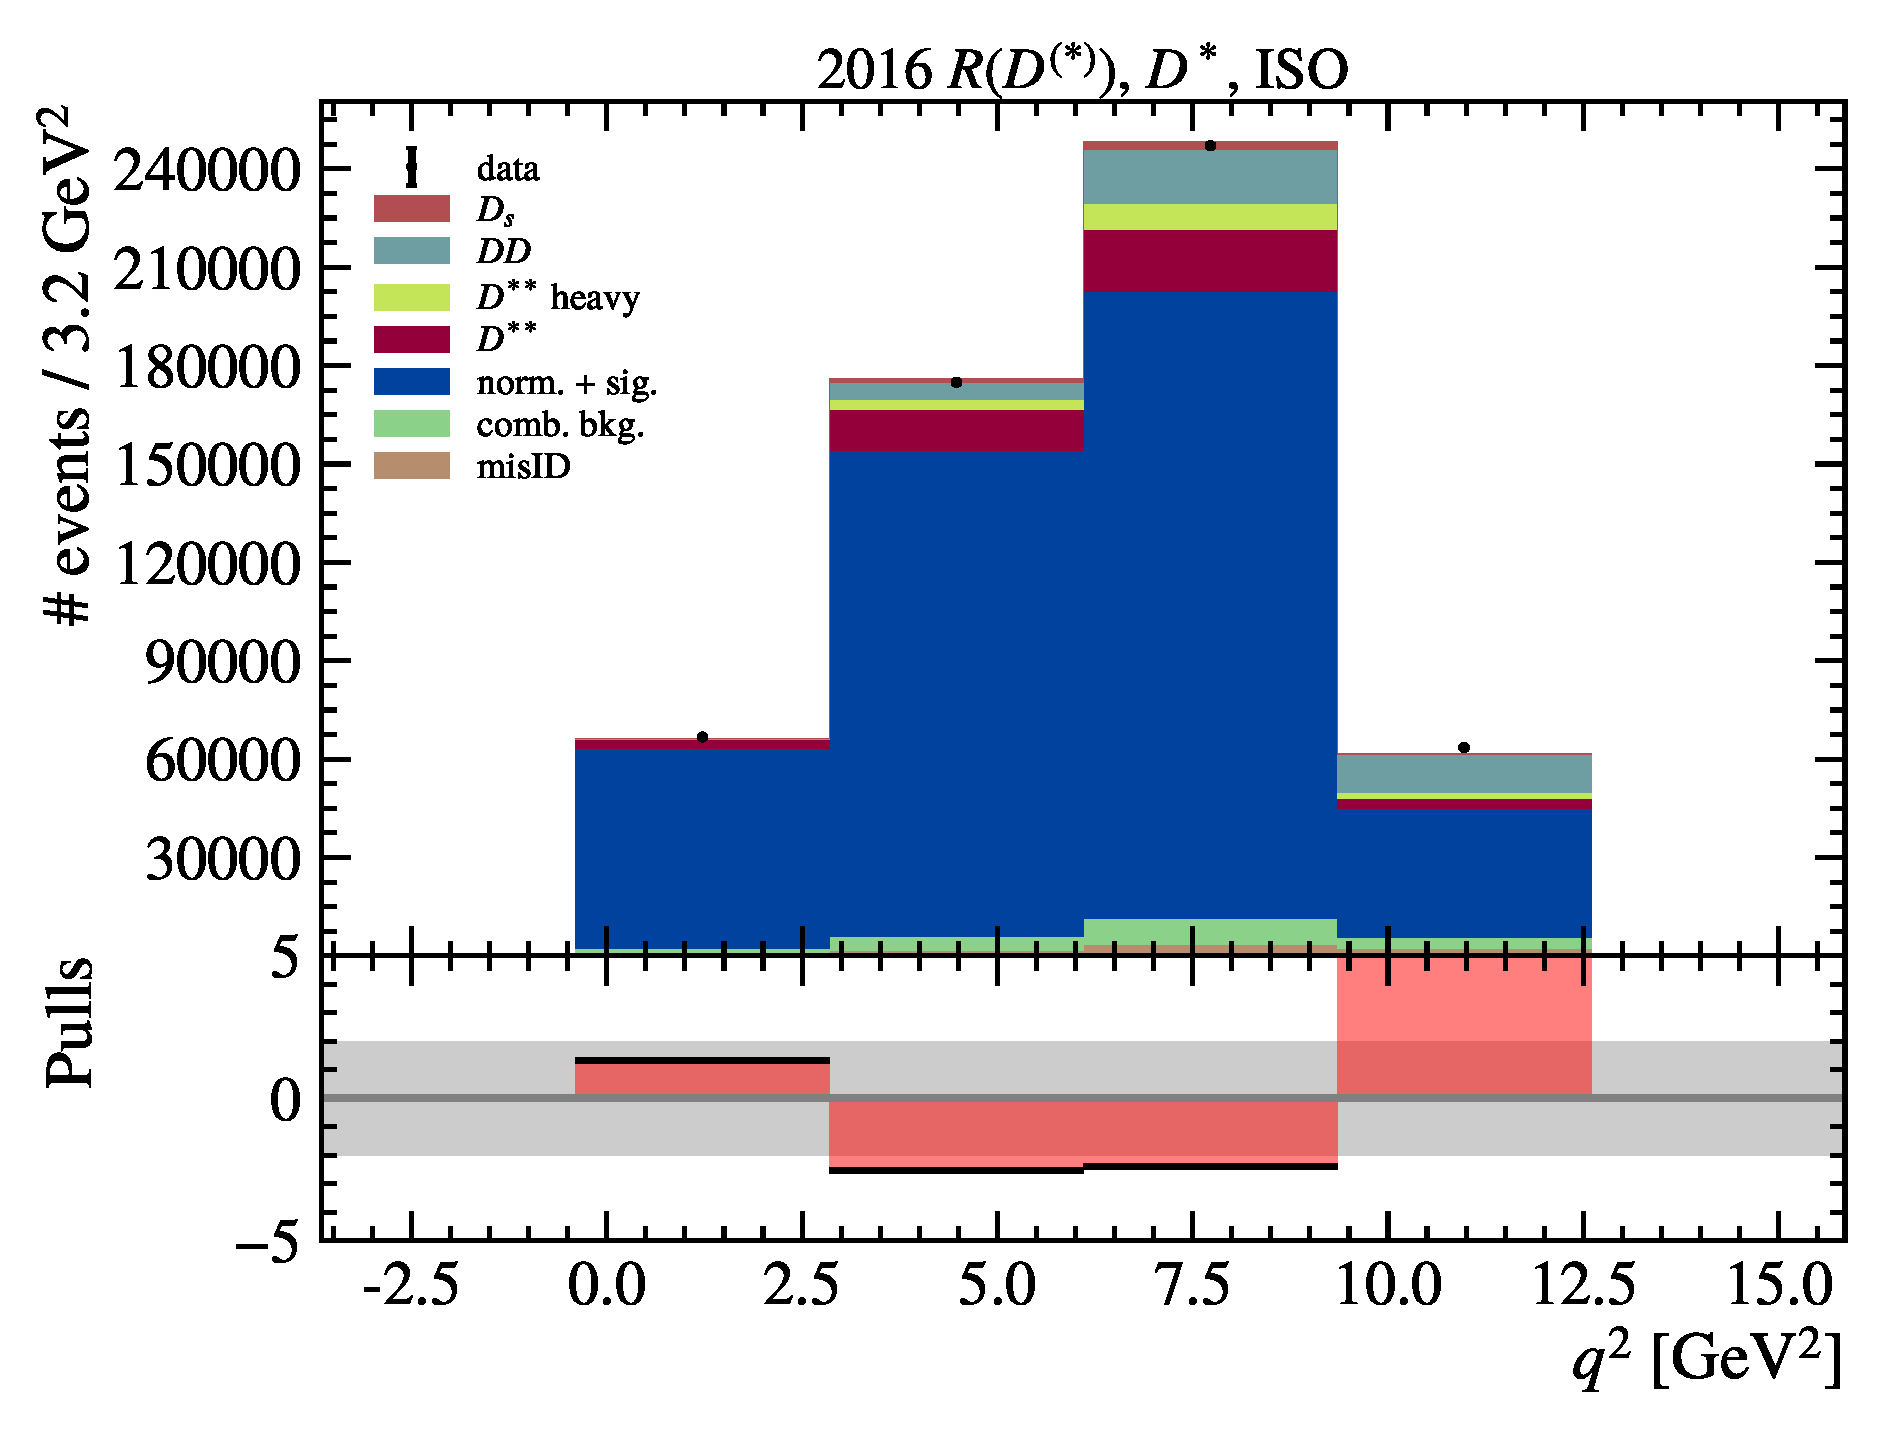
\includegraphics[width=0.85\textwidth]{figs-fit/fit_uvsd/fit_result-stacked-Dst-iso-q2.pdf}
        \caption{The nominal fit.}
    \end{subfigure}%
    \begin{subfigure}[t]{0.5\textwidth}
        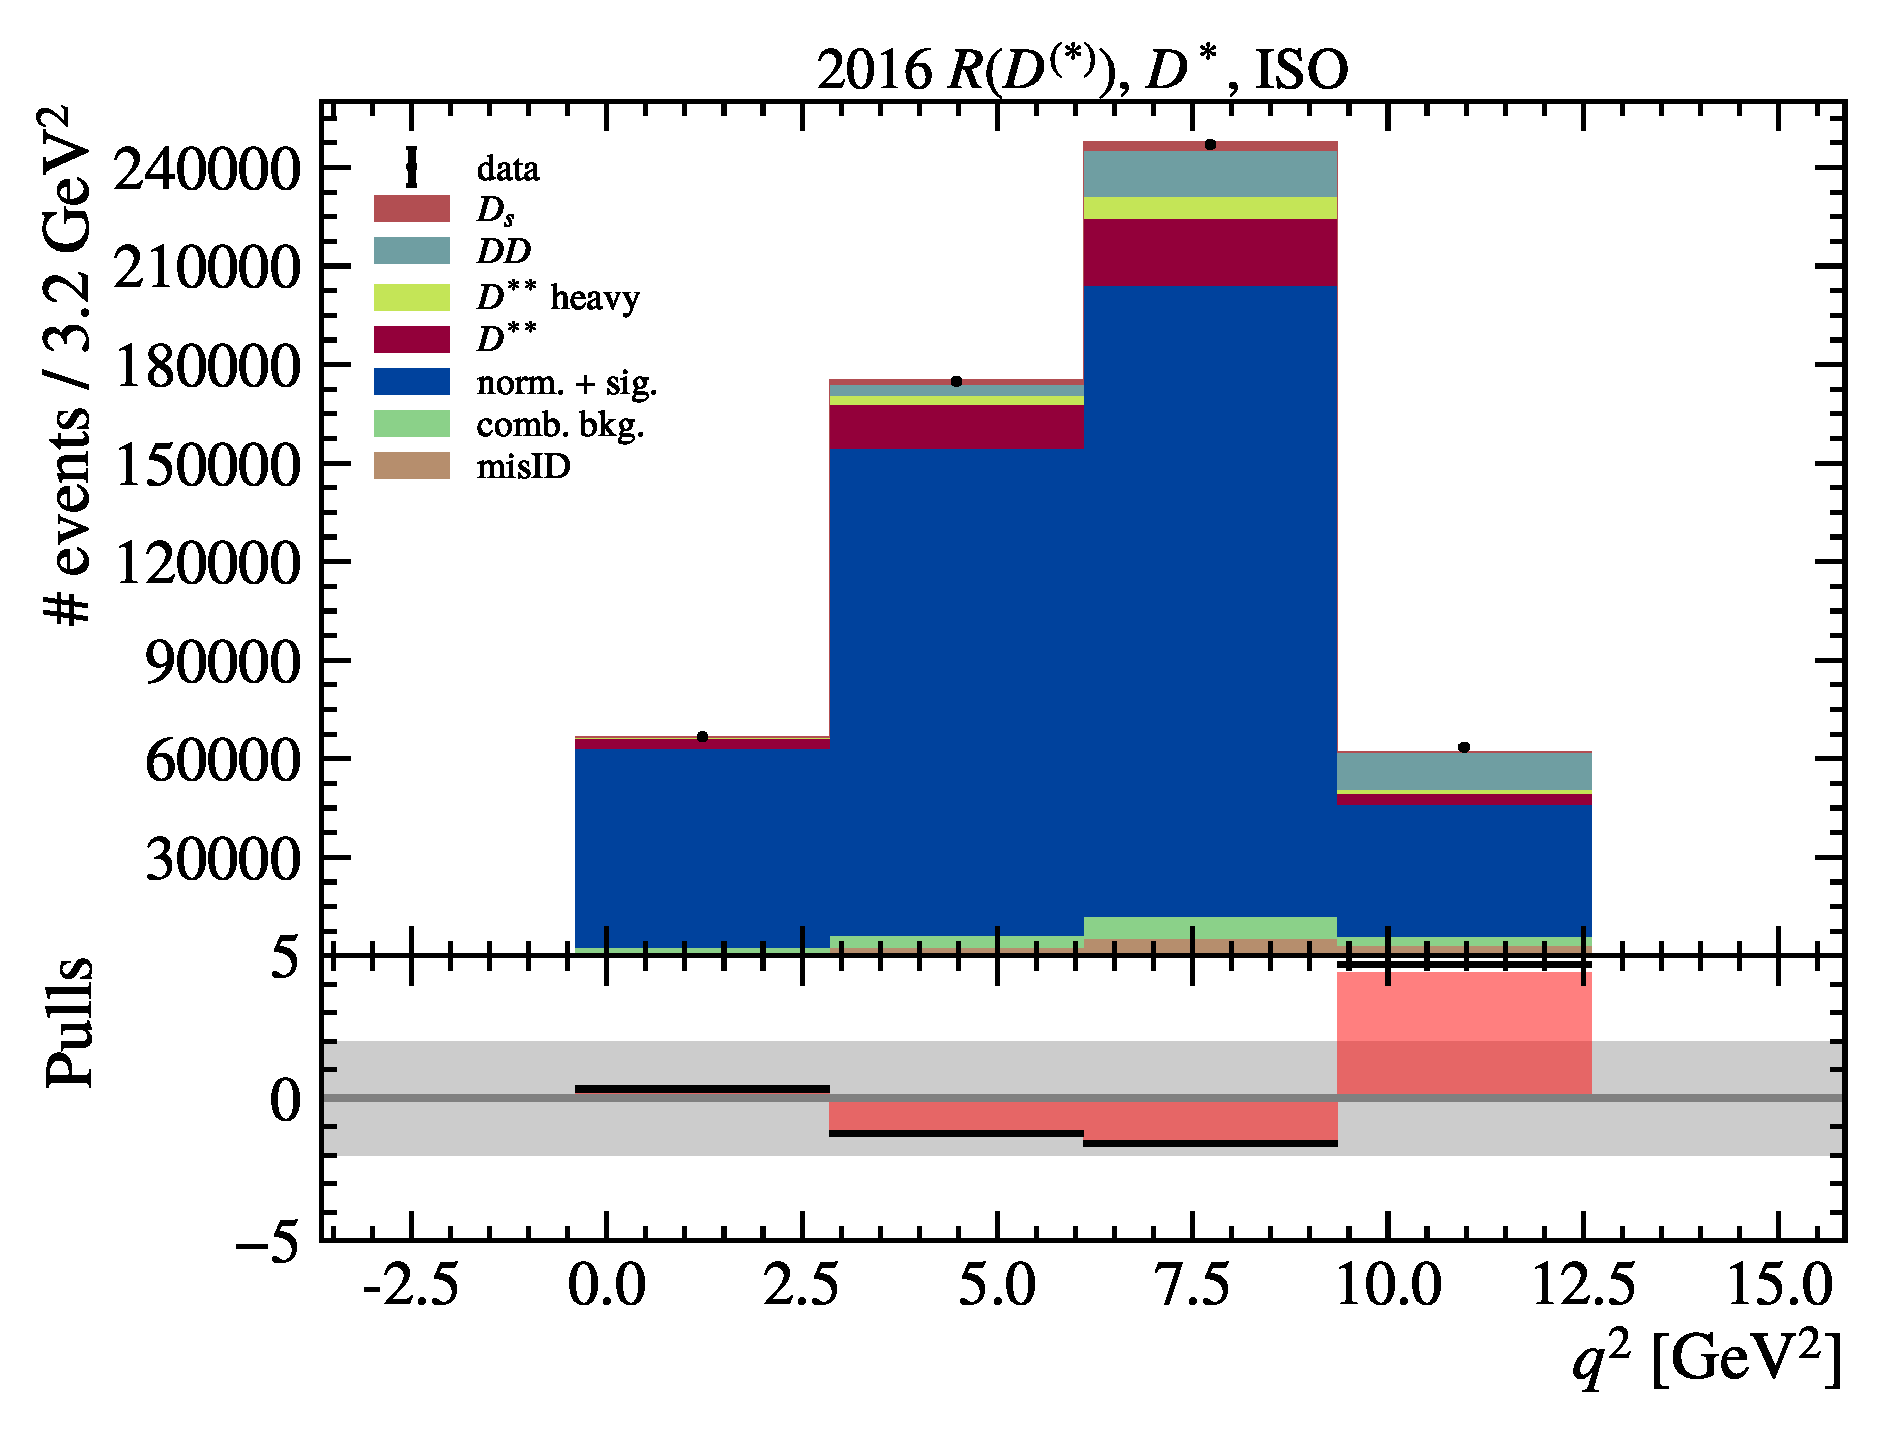
\includegraphics[width=0.85\textwidth]{figs-fit/fit_uvsd/fit_result-stacked-Dst-iso-q2-floating_uvsd.pdf}
        \caption{The fit with $\rho_{DDX,u/d}$ floating.}
    \end{subfigure}

    \caption{
        Allowing the $DDX$ relative fraction $\rho_{DDX,u/d}$ to float in the
        signal fit to float seemingly improves fit quality,
        but the signal are now completely absorbed in the $DDX$ components.
        Only the \Dstar channel fit is shown as it shows the most improvements
        in terms of pulls.
    }
    \label{fig:fit-float-uvsd}
\end{figure}

Therefore, these background shape parameters are obtained with a
\emph{control fit},
a simultaneous fit to the 1OS, 2OS, and DD control skims with six fit channels
(a \Dz and a \Dstar channel for each control skim),
and imported back to the signal fit at the fitted values with either
fitted errors as constraints (for \Dstst shape parameters) or fully fixed
(for $DDX$ shape parameters).
To be more precise,
the fit procedure is broken into 3 steps:

\begin{enumerate}
    \item \textbf{Pre-control}:
        Performed on control skims (1OS, 2OS, DD).
        In this step, all but the \Kstar shape variations are turned off.
    \item \textbf{Control}:
        Also performed on control skims (1OS, 2OS, DD).
        All but the signal and normalization shape variations are turned on.
        The fitted parameters from previous steps are loaded along with their
        errors as a starting point for the control fit.
    \item \textbf{Signal}:
        Performed on signal sample (ISO).
        The variations in the control fit for $D^{**}, D_H^{**}$, and misID DiF
        are loaded as constraints to the signal fit;
        the $DDX$ variations are fixed to the fitted value from the previous
        step.
\end{enumerate}
The terms such as ``\Kstar variations'' and ``misID DiF'' will be defined later.

Both the signal and the control fit are binned extended maximum likelihood
template fits,
with a fitter based on the \HistFactory fitter
used in the pathfinder run 1 \RDX analysis described in
\cite{LHCb-ANA-2020-056}\footnote{
    With code refactored and dependencies updated to enhance readability and
    configurability,
    but the fit model is largely the same.
}.
% Fit variables, include binning
The fit templates are three-dimensional correlation-preserving
histograms of \mmSq, \el, and \qSq,
with binning scheme listed in \cref{tab:fit-vars-binning}.
Events outside the binning ranges of the fit variables are cut out to avoid
potential impact of under/overflow bins on the fitter.
To account for external constraints on fit parameters or uncertainties on
modeling of certain backgrounds,
additional shape variations are introduced on most templates
(i.e. all but the \Dstar combinatorial template have some shape variations which
will be discussed later).

\begin{table}[!htb]
    \centering
    \caption{
        Fit variables and their binnings,
        obtained by the rest frame approximation technique as described
        in \cref{appx:rfa}.
    }
    \label{tab:fit-vars-binning}
    \begin{tabular}{c|l}
        \toprule
        {\bf Variable} & {\bf Binning} \\
        \midrule
        \mmSq [\GeVSq] & 43, -2 -- 10.9 \\
        \el [MeV]      & 34, 100 -- 2650 \\
        \qSq [\GeVSq]  & 4, -0.4 -- 12.6 \\
        \bottomrule
    \end{tabular}
\end{table}

% Pointer to later subsections
The remainder of this chapter is organized as following:
a description on template generation,
followed by a discussion on all components of fit templates,
is described in \cref{ref:fit:tmpl}.
The fit template shape variations are explained in
\cref{ref:fit:var}.
The blinded fitted results are provided in
\cref{ref:fit:results}.


\section{Fit templates}
\label{ref:fit:tmpl}

This selection describes generation of fit templates,
followed by comments on the characteristics of the templates and the
normalization factors controlling the yields of the templates.
There are a total of 37 templates in \Dz channel and 24 in \Dstar channel,
with some templates generated with the decays that contribute to both
channels.
For a brief overview of the templates,
\cref{tab:fit-templates-d0,tab:fit-templates-dst} may be used.
The normalization factors for the signal fit are summarized in
\cref{tab:fit-norm-fact-d0,tab:fit-norm-fact-dst} for the \Dz and \Dstar channel
accordingly and will be documented in the next subsections.
These normalization factors are color-coded as:
\begin{itemize}
    \item \textbf{\textcolor{black}{black}}:
        an unconstrained factor,
        implemented with a \HistFactory\ \smalltt{NormFactor}.
    \item \textbf{\textcolor{red}{red}}:
        a fixed factor,
        also implemented with the \smalltt{NormFactor}.
    \item \textbf{\textcolor{blue}{blue}}:
        a factor with a Gaussian constraint
        where the nominal value is $\mu$ and the standard deviation $\sigma$.
        The fitter reports the \emph{variation} of the factor with an $\alpha$
        parameter such that when the underlying parameter is at the nominal
        value $\mu$, the associated $\alpha = 0$;
        when the underlying parameter is at $\mu \pm \sigma$, the $\alpha = \pm 1$.
        Implemented with a \HistFactory\ \smalltt{OverallSys}.
    \item \textbf{\textcolor{magenta}{magenta}}:
        a fixed \smalltt{OverallSys} factor.
        Typically such a factor is \emph{constrained} in the control fit and
        loaded as a \emph{fixed} factor in the signal fit.
\end{itemize}


% vim: set ft=none:


% Generated in umd-lhcb/rdx-run2-analysis/fit:
%   with: make tab-fit-templates
%% D0
\begin{table}[!htb]
    \caption{Fit templates included in the \Dz channel.}
    \label{tab:fit-templates-d0}
    \footnotesize
    \centering

\begin{tabular}{lllrr}
\toprule
 \textbf{Decay mode}                                                                  & \textbf{Run 2 \texttt{process}}   & \textbf{Alias in fitter}   &   \textbf{Variations} &   \textbf{Index} \\
\midrule
 $B^- \rightarrow D^0 \mu^- \overline{\nu}_\mu$                                       & \texttt{D0Mu}                     & \texttt{D\_Dmu}            &                     5 &                1 \\
 $\overline{B}^0 \rightarrow D^{*+} \mu^- \overline{\nu}_\mu$                         & \texttt{DstMu}                    & \texttt{D\_dDstmu}         &                    10 &                2 \\
 $B^- \rightarrow D^{*0} \mu^- \overline{\nu}_\mu$                                    & \texttt{Dst0Mu}                   & \texttt{D\_uDstmu}         &                    10 &                3 \\
 $B^- \rightarrow D^0 \tau^- \overline{\nu}_\tau$                                     & \texttt{D0Tau}                    & \texttt{D\_Dtau}           &                     5 &                4 \\
 $\overline{B}^0 \rightarrow D^{*+} \tau^- \overline{\nu}_\tau$                       & \texttt{DstTau}                   & \texttt{D\_dDsttau}        &                    10 &                5 \\
 $B^- \rightarrow D^{*0} \tau^- \overline{\nu}_\tau$                                  & \texttt{Dst0Tau}                  & \texttt{D\_uDsttau}        &                    10 &                6 \\
 $\overline{B}^0 \rightarrow D_1 \mu \overline{\nu}_\mu$                              & \texttt{D1ststMu}                 & \texttt{D\_dD1mu}          &                     3 &                7 \\
 $\overline{B}^0 \rightarrow D_1 (\rightarrow D^0 \pi\pi) \mu \overline{\nu}_\mu$     & \texttt{D1ststMuD0PiPi}           & \texttt{D\_dD1mu\_pipi}    &                     3 &                8 \\
 $\overline{B}^0 \rightarrow D^*_2 \mu \overline{\nu}_\mu$                            & \texttt{D2ststMu}                 & \texttt{D\_dD2mu}          &                     3 &                9 \\
 $\overline{B}^0 \rightarrow D'_1 \mu \overline{\nu}_\mu$                             & \texttt{D1pststMu}                & \texttt{D\_dD1pmu}         &                     2 &               10 \\
 $\overline{B}^0 \rightarrow D^*_0 \mu \overline{\nu}_\mu$                            & \texttt{D0ststMu}                 & \texttt{D\_dD0mu}          &                     2 &               11 \\
 $\overline{B} \rightarrow D^{**} (\rightarrow D^{*0} \pi\pi) \mu \overline{\nu}_\mu$ & \texttt{DststHMuDst0}             & \texttt{D\_Dstzpipimu}     &                     1 &               12 \\
 $\overline{B} \rightarrow D^{**} (\rightarrow D^* \pi\pi) \mu \overline{\nu}_\mu$    & \texttt{DststHMuDst}              & \texttt{D\_Dstppipimu}     &                     1 &               13 \\
 $\overline{B} \rightarrow D^{**} (\rightarrow D^0 \pi\pi) \mu \overline{\nu}_\mu$    & \texttt{DststHMuD0}               & \texttt{D\_Dpipimu}        &                     1 &               14 \\
 $B^- \rightarrow D_1^0 \mu \overline{\nu}_\mu$                                       & \texttt{D1stst0Mu}                & \texttt{D\_uD1mu}          &                     3 &               15 \\
 $B^- \rightarrow D_1^0 (\rightarrow D^0 \pi\pi) \mu \overline{\nu}_\mu$              & \texttt{D1stst0MuD0PiPi}          & \texttt{D\_uD1mu\_pipi}    &                     3 &               16 \\
 $B^- \rightarrow D_2^{*0} \mu \overline{\nu}_\mu$                                    & \texttt{D2stst0Mu}                & \texttt{D\_uD2mu}          &                     3 &               17 \\
 $B^- \rightarrow {D'_1}^0 \mu \overline{\nu}_\mu$                                    & \texttt{D1pstst0Mu}               & \texttt{D\_uD1pmu}         &                     2 &               18 \\
 $B^- \rightarrow {D^*_0}^0 \mu \overline{\nu}_\mu$                                   & \texttt{D0stst0Mu}                & \texttt{D\_uD0mu}          &                     2 &               19 \\
 $\overline{B}_s \rightarrow D_{s2}^* \mu \overline{\nu}_\mu$                         & \texttt{Ds2Mu}                    & \texttt{D\_sDs2mu}         &                     3 &               20 \\
 $\overline{B}_s \rightarrow D'_{s1} \mu \overline{\nu}_\mu$                          & \texttt{Ds1pMu}                   & \texttt{D\_sDs1pmu}        &                     3 &               21 \\
 $\overline{B}^0 \rightarrow D_1 \tau \overline{\nu}_\tau$                            & \texttt{D1ststTau}                & \texttt{D\_dD1tau}         &                     3 &               22 \\
 $\overline{B}^0 \rightarrow D_1 (\rightarrow D^0 \pi\pi) \tau \overline{\nu}_\tau$   & \texttt{D1ststTauD0PiPi}          & \texttt{D\_dD1tau\_pipi}   &                     3 &               23 \\
 $\overline{B}^0 \rightarrow D^*_2 \tau \overline{\nu}_\tau$                          & \texttt{D2ststTau}                & \texttt{D\_dD2tau}         &                     3 &               24 \\
 $\overline{B}^0 \rightarrow D'_1 \tau \overline{\nu}_\tau$                           & \texttt{D1pststTau}               & \texttt{D\_dD1ptau}        &                     2 &               25 \\
 $\overline{B}^0 \rightarrow D^*_0 \tau \overline{\nu}_\tau$                          & \texttt{D0ststTau}                & \texttt{D\_dD0tau}         &                     2 &               26 \\
 $B^- \rightarrow D_1^0 \tau \overline{\nu}_\tau$                                     & \texttt{D1stst0Tau}               & \texttt{D\_uD1tau}         &                     3 &               27 \\
 $B^- \rightarrow D_1^0 (\rightarrow D^0 \pi\pi) \mu \overline{\nu}_\tau$             & \texttt{D1stst0TauD0PiPi}         & \texttt{D\_uD1tau\_pipi}   &                     3 &               28 \\
 $B^- \rightarrow D_2^{*0} \tau \overline{\nu}_\tau$                                  & \texttt{D2stst0Tau}               & \texttt{D\_uD2tau}         &                     3 &               29 \\
 $B^- \rightarrow {D'_1}^0 \tau \overline{\nu}_\tau$                                  & \texttt{D1pstst0Tau}              & \texttt{D\_uD1ptau}        &                     2 &               30 \\
 $B^- \rightarrow {D^*_0}^0 \tau \overline{\nu}_\tau$                                 & \texttt{D0stst0Tau}               & \texttt{D\_uD0tau}         &                     2 &               31 \\
 $\overline{B}^0 \rightarrow D^0 D_q (\rightarrow \mu \overline{\nu}_\mu X') X$       & \texttt{dDDMu}                    & \texttt{D\_dDDmu}          &                     3 &               32 \\
 $B^- \rightarrow D^0 D_q (\rightarrow \mu \overline{\nu}_\mu X') X$                  & \texttt{uDDMu}                    & \texttt{D\_uDDmu}          &                     3 &               33 \\
 $\overline{B}^0 \rightarrow D^0 D_q (\rightarrow \tau \overline{\nu}_\tau X') X$     & \texttt{dDDTau}                   & \texttt{D\_dDDtau}         &                     0 &               34 \\
 $B^- \rightarrow D^0 D_q (\rightarrow \tau \overline{\nu}_\tau X') X$                & \texttt{uDDTau}                   & \texttt{D\_uDDtau}         &                     0 &               35 \\
 $B^-$ comb. bkg.                                                                     & \texttt{BComb}                    & \texttt{D\_comb}           &                     1 &               36 \\
 misID.                                                                               & \texttt{misID}                    & \texttt{D\_misID}          &                     1 &               37 \\
\bottomrule
\end{tabular}

\end{table}


%% Dst
\begin{table}[!htb]
    \caption{Fit templates included in the \Dstar channel.}
    \label{tab:fit-templates-dst}
    \footnotesize
    \centering

\begin{tabular}{lllrr}
\toprule
 \textbf{Decay mode}                                                               & \textbf{Run 2 \texttt{process}}   & \textbf{Alias in fitter}   &   \textbf{Variations} &   \textbf{Index} \\
\midrule
 $\overline{B}^0 \rightarrow D^{*+} \mu^- \overline{\nu}_\mu$                      & \texttt{DstMu}                    & \texttt{Dst\_sigmu}        &                    10 &                1 \\
 $\overline{B}^0 \rightarrow D^{*+} \tau^- \overline{\nu}_\tau$                    & \texttt{DstTau}                   & \texttt{Dst\_sigtau}       &                    10 &                2 \\
 $\overline{B}^0 \rightarrow D_1 \mu \overline{\nu}_\mu$                           & \texttt{D1ststMu}                 & \texttt{Dst\_D1}           &                     3 &                3 \\
 $\overline{B}^0 \rightarrow D^*_2 \mu \overline{\nu}_\mu$                         & \texttt{D2ststMu}                 & \texttt{Dst\_D2}           &                     3 &                4 \\
 $\overline{B}^0 \rightarrow D'_1 \mu \overline{\nu}_\mu$                          & \texttt{D1pststMu}                & \texttt{Dst\_D1p}          &                     2 &                5 \\
 $\overline{B} \rightarrow D^{**} (\rightarrow D^* \pi\pi) \mu \overline{\nu}_\mu$ & \texttt{DststHMuDst}              & \texttt{Dst\_D2Smu}        &                     1 &                6 \\
 $B^- \rightarrow D_1^0 \mu \overline{\nu}_\mu$                                    & \texttt{D1stst0Mu}                & \texttt{Dst\_uD1}          &                     3 &                7 \\
 $B^- \rightarrow D_2^{*0} \mu \overline{\nu}_\mu$                                 & \texttt{D2stst0Mu}                & \texttt{Dst\_uD2}          &                     3 &                8 \\
 $B^- \rightarrow {D'_1}^0 \mu \overline{\nu}_\mu$                                 & \texttt{D1pstst0Mu}               & \texttt{Dst\_uD1p}         &                     2 &                9 \\
 $\overline{B}_s \rightarrow D_{s2}^* \mu \overline{\nu}_\mu$                      & \texttt{Ds2Mu}                    & \texttt{Dst\_Ds2}          &                     3 &               10 \\
 $\overline{B}_s \rightarrow D'_{s1} \mu \overline{\nu}_\mu$                       & \texttt{Ds1pMu}                   & \texttt{Dst\_Ds1p}         &                     3 &               11 \\
 $\overline{B}^0 \rightarrow D_1 \tau \overline{\nu}_\tau$                         & \texttt{D1ststTau}                & \texttt{Dst\_D1tau}        &                     3 &               12 \\
 $\overline{B}^0 \rightarrow D^*_2 \tau \overline{\nu}_\tau$                       & \texttt{D2ststTau}                & \texttt{Dst\_D2tau}        &                     3 &               13 \\
 $\overline{B}^0 \rightarrow D'_1 \tau \overline{\nu}_\tau$                        & \texttt{D1pststTau}               & \texttt{Dst\_D1ptau}       &                     2 &               14 \\
 $B^- \rightarrow D_1^0 \tau \overline{\nu}_\tau$                                  & \texttt{D1stst0Tau}               & \texttt{Dst\_uD1tau}       &                     3 &               15 \\
 $B^- \rightarrow D_2^{*0} \tau \overline{\nu}_\tau$                               & \texttt{D2stst0Tau}               & \texttt{Dst\_uD2tau}       &                     3 &               16 \\
 $B^- \rightarrow {D'_1}^0 \tau \overline{\nu}_\tau$                               & \texttt{D1pstst0Tau}              & \texttt{Dst\_uD1ptau}      &                     2 &               17 \\
 $\overline{B}^0 \rightarrow D^* D_q (\rightarrow \mu \overline{\nu}_\mu X') X$    & \texttt{dDDMu}                    & \texttt{Dst\_dDDmu}        &                     3 &               18 \\
 $B^- \rightarrow D^* D_q (\rightarrow \mu \overline{\nu}_\mu X') X$               & \texttt{uDDMu}                    & \texttt{Dst\_uDDmu}        &                     3 &               19 \\
 $\overline{B}^0 \rightarrow D^* D_q (\rightarrow \tau \overline{\nu}_\tau X') X$  & \texttt{dDDTau}                   & \texttt{Dst\_dDDtau}       &                     0 &               20 \\
 $B^- \rightarrow D^* D_q (\rightarrow \tau \overline{\nu}_\tau X') X$             & \texttt{uDDTau}                   & \texttt{Dst\_uDDtau}       &                     0 &               21 \\
 $\overline{B}^0$ comb. bkg.                                                       & \texttt{BComb}                    & \texttt{Dst\_comb}         &                     1 &               22 \\
 misID.                                                                            & \texttt{misID}                    & \texttt{Dst\_misID}        &                     1 &               23 \\
 $D^*$ comb. bkg.                                                                  & \texttt{DstComb}                  & \texttt{Dst\_doug}         &                     0 &               24 \\
\bottomrule
\end{tabular}

\end{table}



The data-driven templates,
namely \muon misID and combinatorial background templates,
are discussed first in \cref{ref:fit:tmpl:misid,ref:fit:tmpl:comb}.
They are used to estimate both the shapes and the yields of the misID and
combinatorial backgrounds.

The rest are all MC templates which can be categorized into signal,
normalization, feed downs from \Dstst/heavy \Dstst/$D^{**}_s$, and contributions
from $DDX$ decay modes.
Only the shapes of these templates are taken as the shapes of the fit variables
of these decays.
All categories share the same selection requirement as discussed in
\cref{ref:sel:mc}.
Additional global weights to account for emulation of trigger and PID
(\cref{ref:mc-emulation}),
form factor reweighting (\cref{ref:mc-cor:ff}, whenever applicable),
and corrections to detector responses (\cref{ref:mc-cor:init,ref:mc-cor:final})
are also applied according to \cref{eqn:mc-wts},
with weight-capping strategy specified as:

\begin{equation}
    w_\text{tot} = \underbrace{\left(
            w_\text{trigger} \cdot w_\text{PID} \cdot
            \overbrace{
                w_\text{tracking} \cdot w_{\jpsi\kaon}
            }^\text{initial weight}
        \right)}_\text{capped at 10} \;\; \times
        \underbrace{w_\text{form factor}}_{\substack{
            \text{capped at} \\
            \text{50 for \Dz and \Dstar} \\
            \text{10 for $D^{**}$}
        }} \times \;\;
        \underbrace{
            {\textstyle\prod_i} w_\text{final weight,step $i$}
        }_\text{capped at 10}
        \label{eqn:mc-wts}
\end{equation}


\subsection{Muon misID backgrounds}
\label{ref:fit:tmpl:misid}

The \muon misID templates,
shown in \cref{fig:misid-vs-sig},
representing contributions from non-\muon tracks passing the \muon
identification requirements in ``real'' \muon samples,
are generated from the fake \muon control sample
(as in \cref{ref:sel:data:fake-mu}) with an unfolding technique.
First conceived in \cite{LHCb-ANA-2016-059}, the unfolding technique
consists of the following steps:

\begin{figure}[!htb]
    \centering
    \begin{subfigure}{0.9\textwidth}
        \centering
        \caption{
            \muon misID vs. $\Bm \rightarrow \Dz\taum\neutb$ in \Dz channel.
        }
    \end{subfigure}

    \begin{subfigure}{0.9\textwidth}
        \centering
        \caption{
            \muon misID vs. $\Bzb \rightarrow \Dstarp\taum\neutb$ in \Dstar channel.
        }
    \end{subfigure}

    \caption{
        Comparison between misID and the signal templates in their
        respective channel.
    }
    \label{fig:misid-vs-sig}
\end{figure}

\begin{enumerate}
    \item Tag the fake \muon sample into $\pi$, $K$, $p$,
        $e$, and ghost\footnote{
            ``Ghost'' refers to tracks formed by random combination of hits.
        }-like species with the selection requirements listed in
        \cref{tab:selection-for-tagged-species}.
        Denote tagged species with a hat:
        $\hat{t} \in \{\hat{\pi}, \hat{K}, \hat{p}, \hat{e}, \hat{g}\}$,

    \item Obtain the efficiency for a track of true species $t$ passing \muon
        acceptance to be classified as a tagged species $\hat{t}'$
        (where $t$ and $t'$ can be the same species, e.g. a true electron
        (passing \muon acceptance) classified as a tagged electron):
        $\misEff[t]{\hat{t}'}$.
        These efficiencies are obtained from \pidcalib for $\pi, K, p, e$ and
        from MC for $g$.

    \item Given the measured yields in the fake \muon sample $\tilde{n}_{\hat{t}'}
        $ and response matrix
        $M_{\hat{t}', t^{\phantom{}}} = \misEff[t^{\phantom{}}]{\hat{t}'}$,
        % NOTE: The subscript of M is indeed tag, true!!! NOT true, tag!!!
        unfold the true yields $\tilde{n}_{t}$.
        A Bayesian unfolding (iterative unfolding, \cite{DAGOSTINI1995487})
        algorithm is used to obtain the true yields and subsequently the
        efficiencies of a tagged
        $\hat{t}'$ being a true $t$: $\misEff[\hat{t}']{t}$.

      \item Find $\misEff[\hat{t}']{\hat{\mu}}$,
        the transfer factor from the fake \muon sample
        (of tagged species $\hat{t}'$) to the ``real'' \muon
        samples\footnote{
            A subtlety is that here ``real'' \muon refers to the samples passing
            \muon PID cuts listed in \cref{ref:sel:data:rs}.
            Because the \muon-like particles are selected by a set of cuts,
            a hat is placed on \muon ($\hat{\mu}$!)
            to remind the reader that this sample is nothing but a \muon tag
            and is unrelated to the \muon-enriched sample (true \muon) as used
            by \pidcalib.
        },
        based on
        \begin{itemize}
            \item the efficiencies obtained in the step above,
            \item the efficiency of a track of true species $t$ that falls
                within \muon acceptance to also pass the \muon PID cuts
                $\misEff[t_\text{acc}]{\hat{\mu}}$,
            \item and the efficiency of $t_\text{acc}$ to \emph{fail} the \muon
                PID:
                $\misEff[t_\text{acc}]{t}$.
        \end{itemize}

        \begin{equation}
            \misEff[\hat{t}']{\hat{\mu}} =
                \sum_{t}
                \frac{\misEff[\hat{t}']{t}}{\misEff[t_\text{acc}]{t}}
                \misEff[t_\text{acc}]{\hat{\mu}}
        \end{equation}
        The last two efficiencies are found from \pidcalib.

    \item Apply $\misEff[\hat{t}']{\hat{\mu}}$ as a weight for each
        tagged species $\hat{t}'$ in the fake \muon sample.
        The weighted yield of tagged species $\hat{t}$ represents the \muon misID
        contributions of $\hat{t}$ to the ``real'' \muon samples.
\end{enumerate}

Comparisons between tagged and unfolded (true) yields of the fake \muon sample
are shown in \cref{fig:unfolding-binning-vars}.
The weighted yields are projected in fit variables with finer binning;
these are shown in \cref{fig:unfolding-fit-vars}.
Some of the efficiencies obtained with \pidcalib are negative; these are shifted
back to a value between $[0, 1]$ with an algorithm described in
\cref{appx:formal:shift-neg-eff}.
A more detailed description of the unfolding procedure is documented in
\cref{appx:unfold-tech}.

% Generated in /misid-unfolding, with the command
%   make plot-rdx-bin_vars-ana-2016
\begin{figure}[!htb]
    \centering
    \begin{subfigure}[b]{0.32\textwidth}
        \centering
        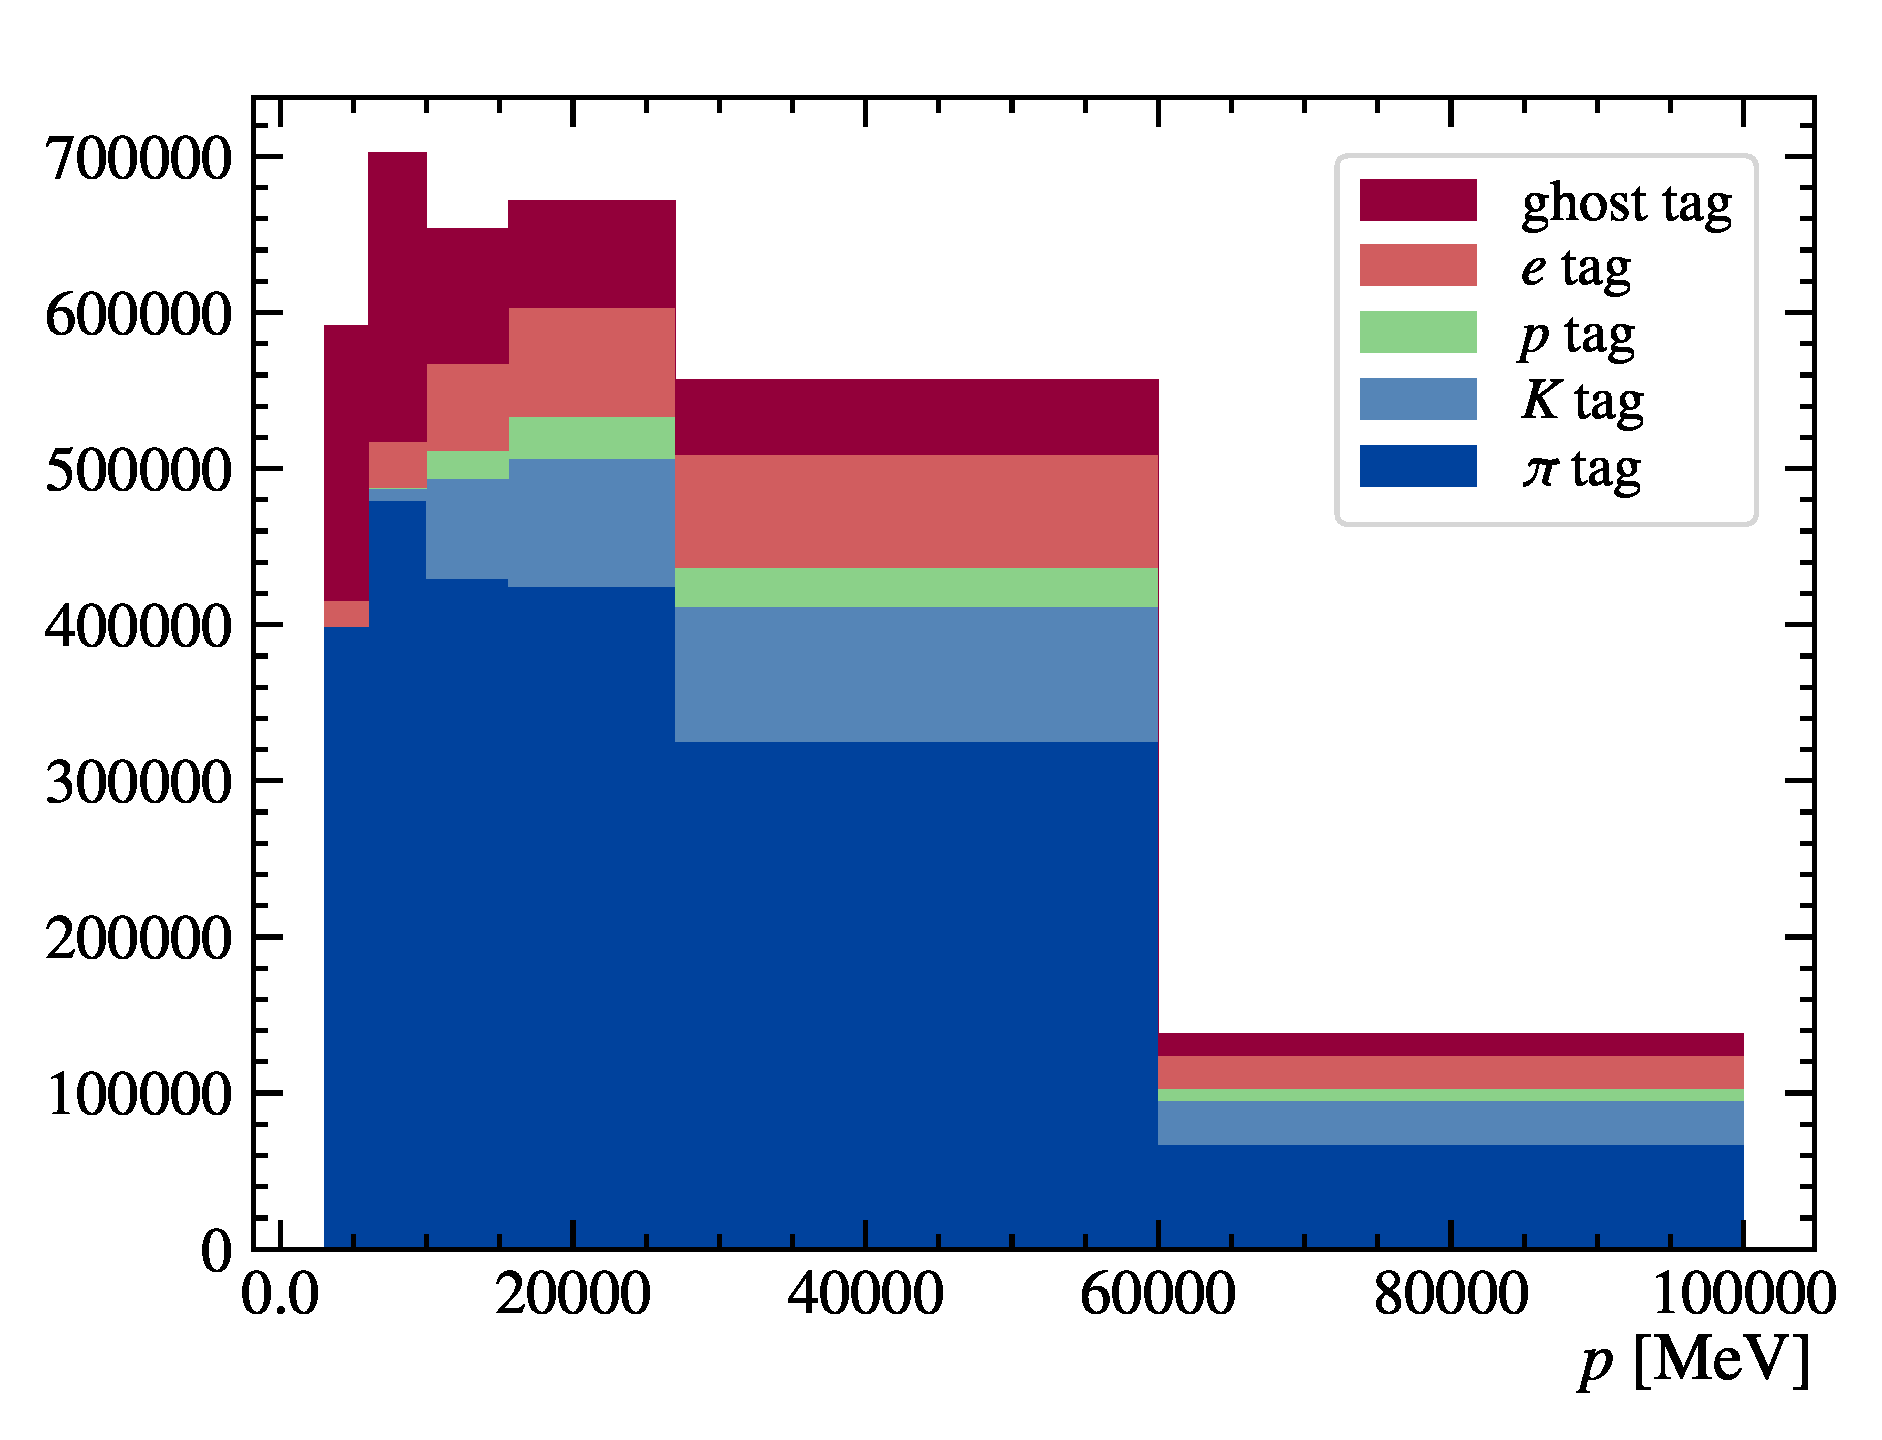
\includegraphics[width=\textwidth]{figs-fit-fit-templates/data-driven-plots/misid/D0-tag_p.pdf}
    \end{subfigure}
    \hfill
    \begin{subfigure}[b]{0.32\textwidth}
        \centering
        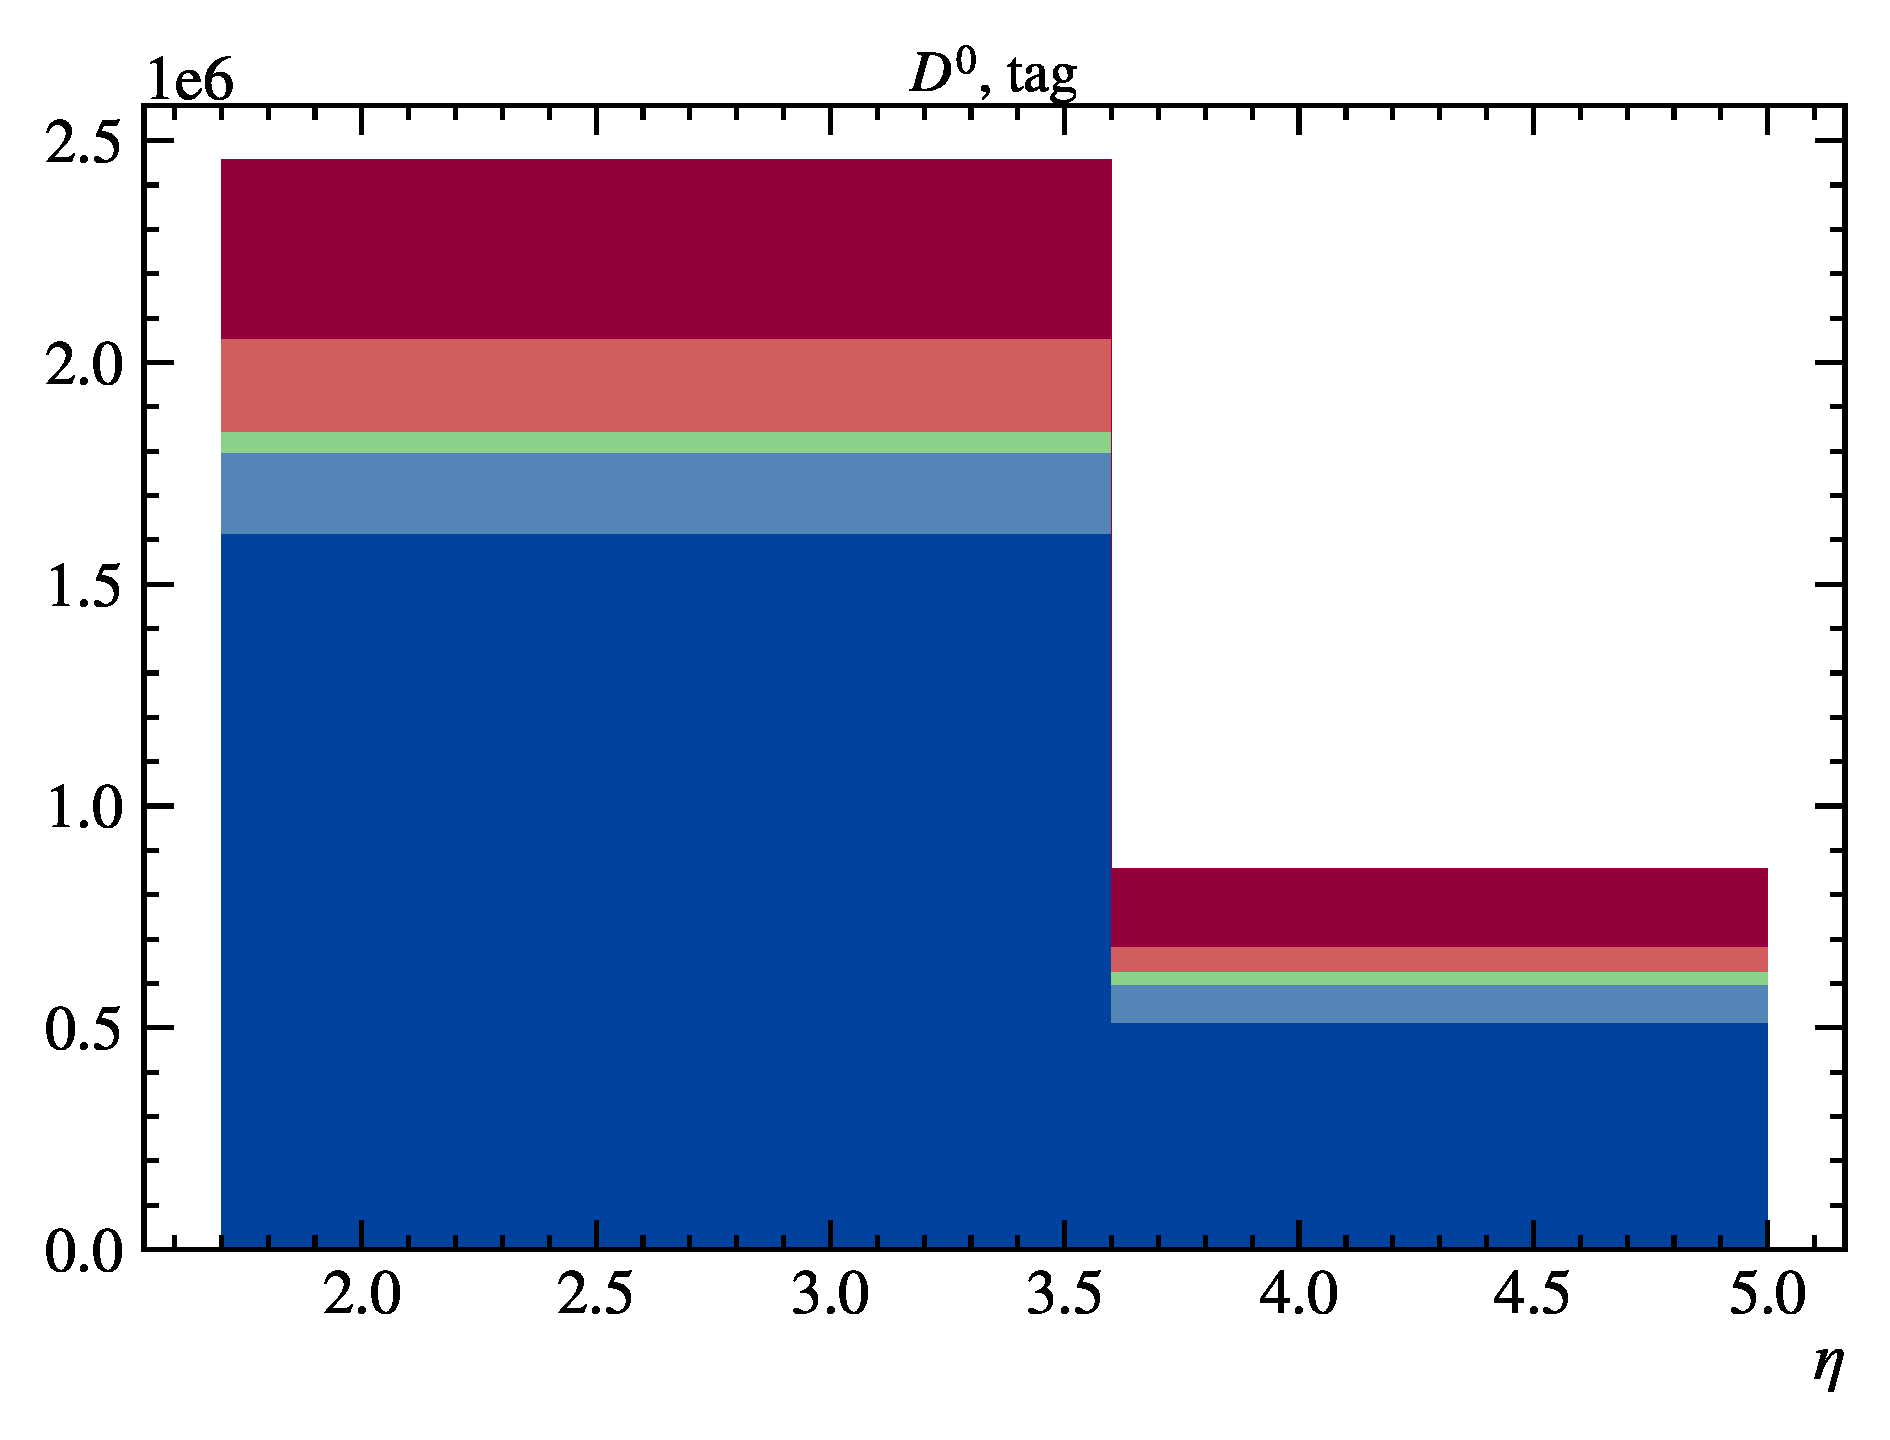
\includegraphics[width=\textwidth]{figs-fit-fit-templates/data-driven-plots/misid/D0-tag_eta.pdf}
    \end{subfigure}
    \hfill
    \begin{subfigure}[b]{0.32\textwidth}
        \centering
        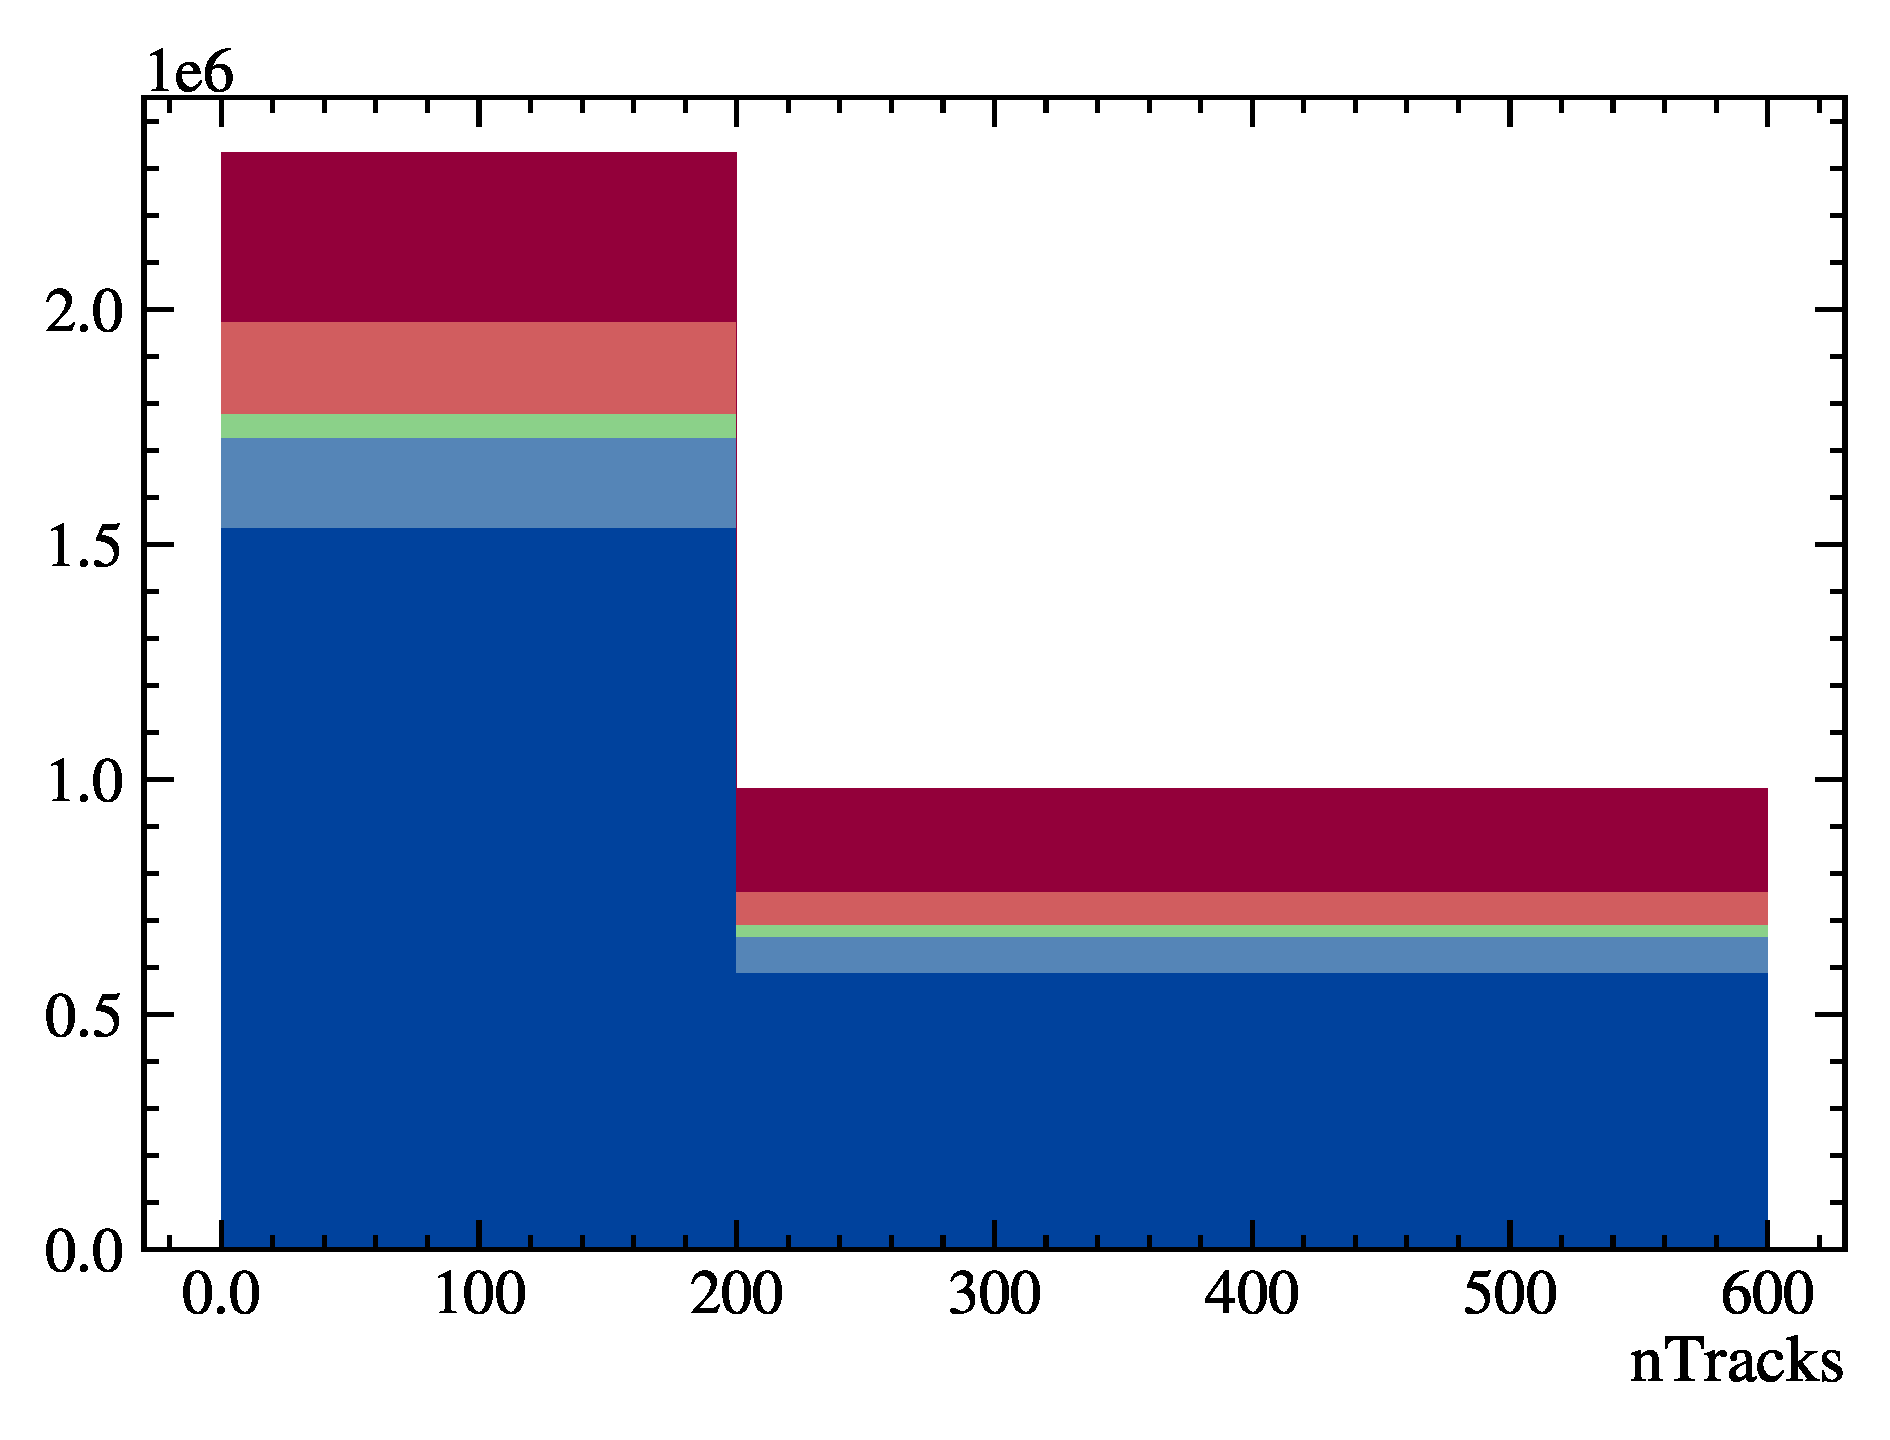
\includegraphics[width=\textwidth]{figs-fit-fit-templates/data-driven-plots/misid/D0-tag_ntracks.pdf}
    \end{subfigure}
    \\
    \begin{subfigure}[b]{0.32\textwidth}
        \centering
        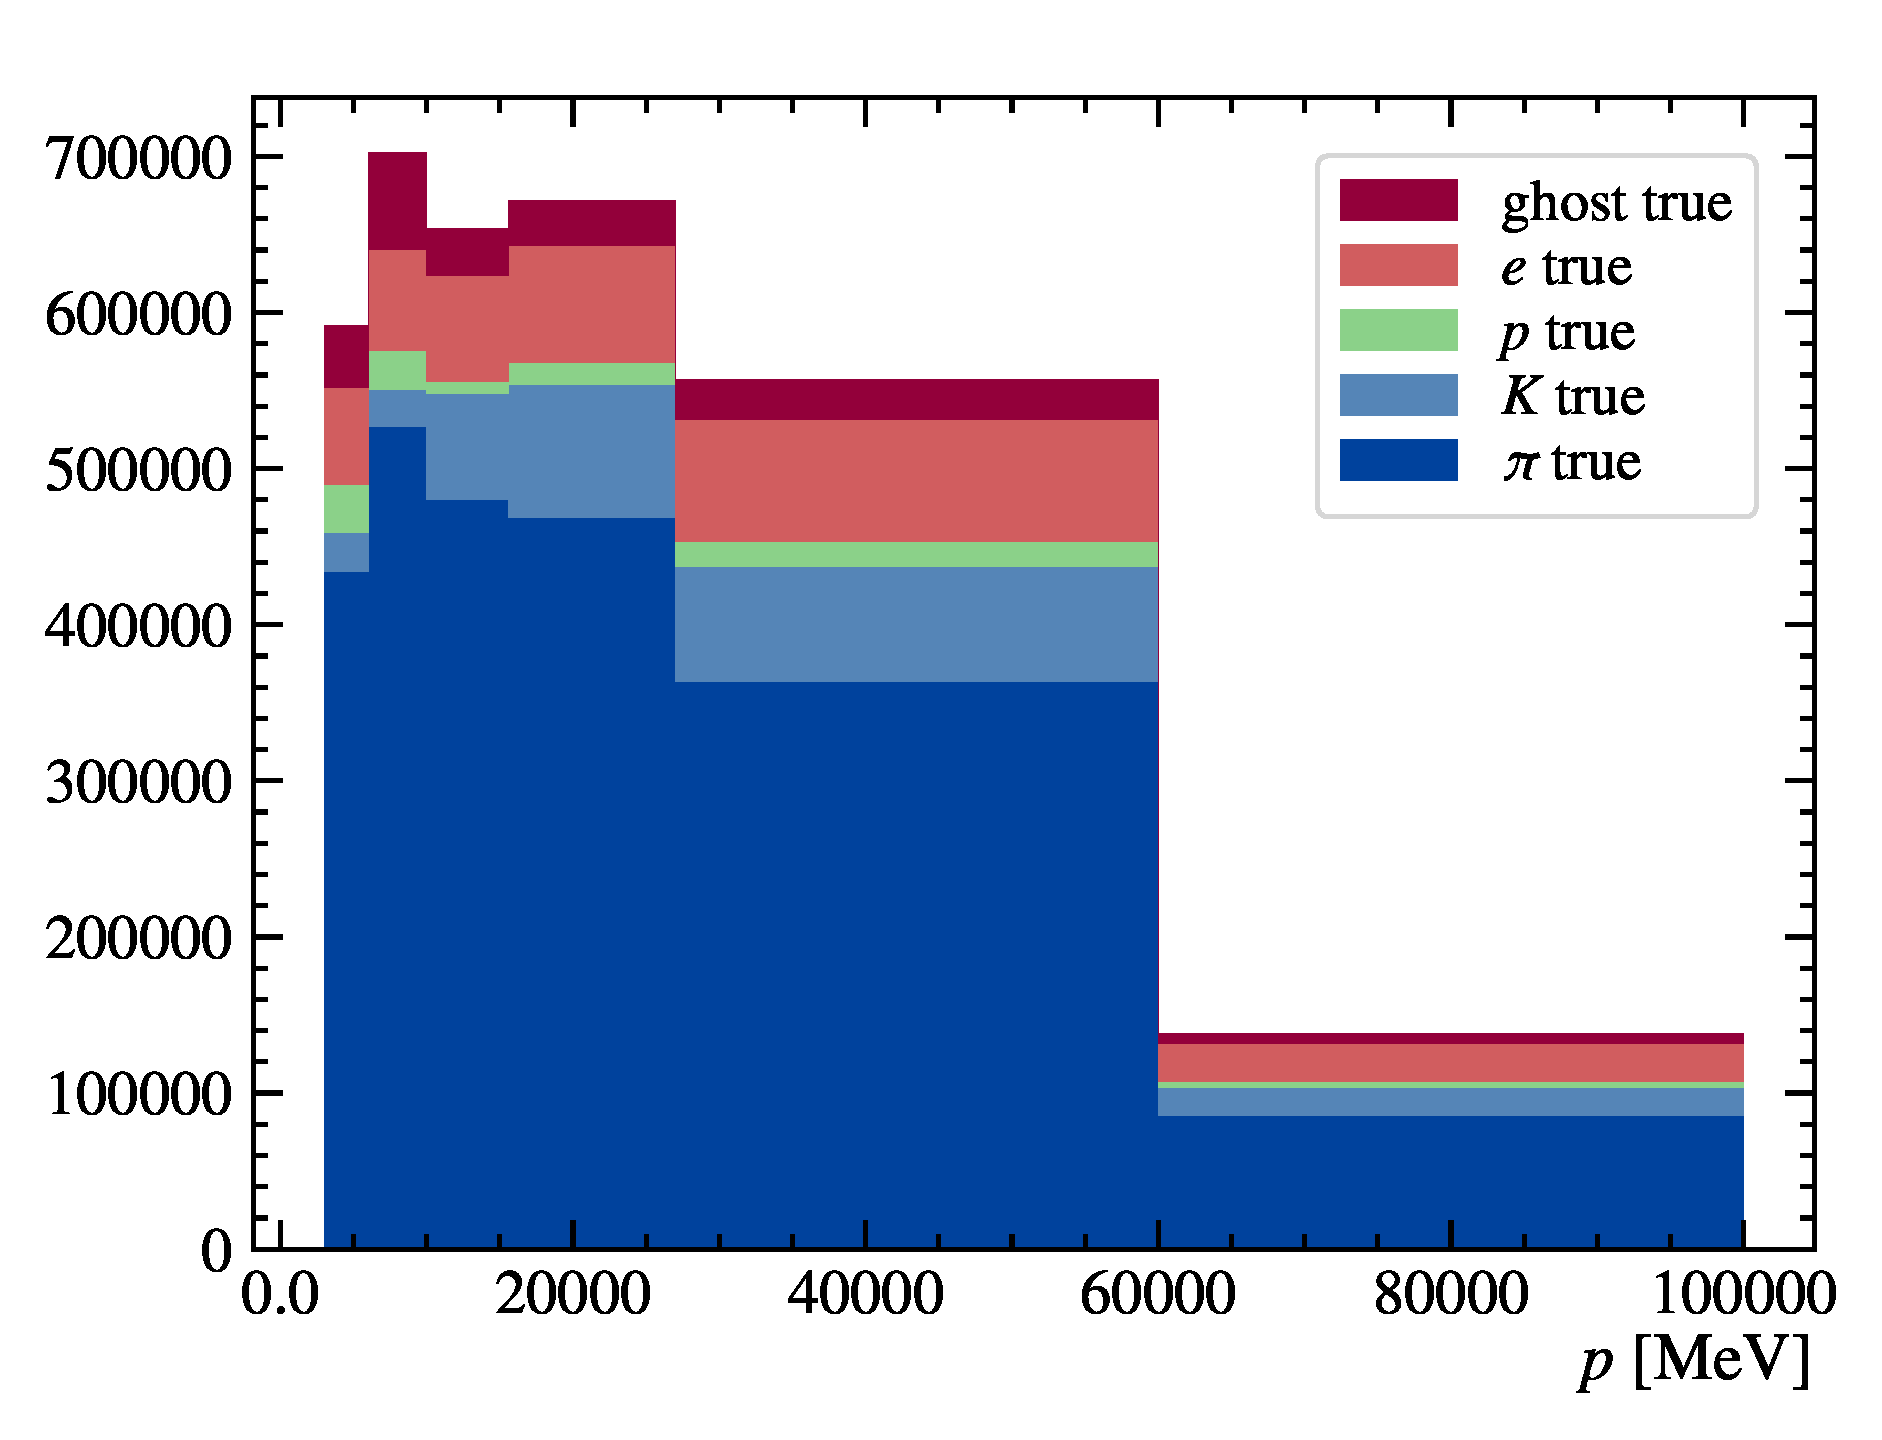
\includegraphics[width=\textwidth]{figs-fit-fit-templates/data-driven-plots/misid/D0-true_p.pdf}
    \end{subfigure}
    \hfill
    \begin{subfigure}[b]{0.32\textwidth}
        \centering
        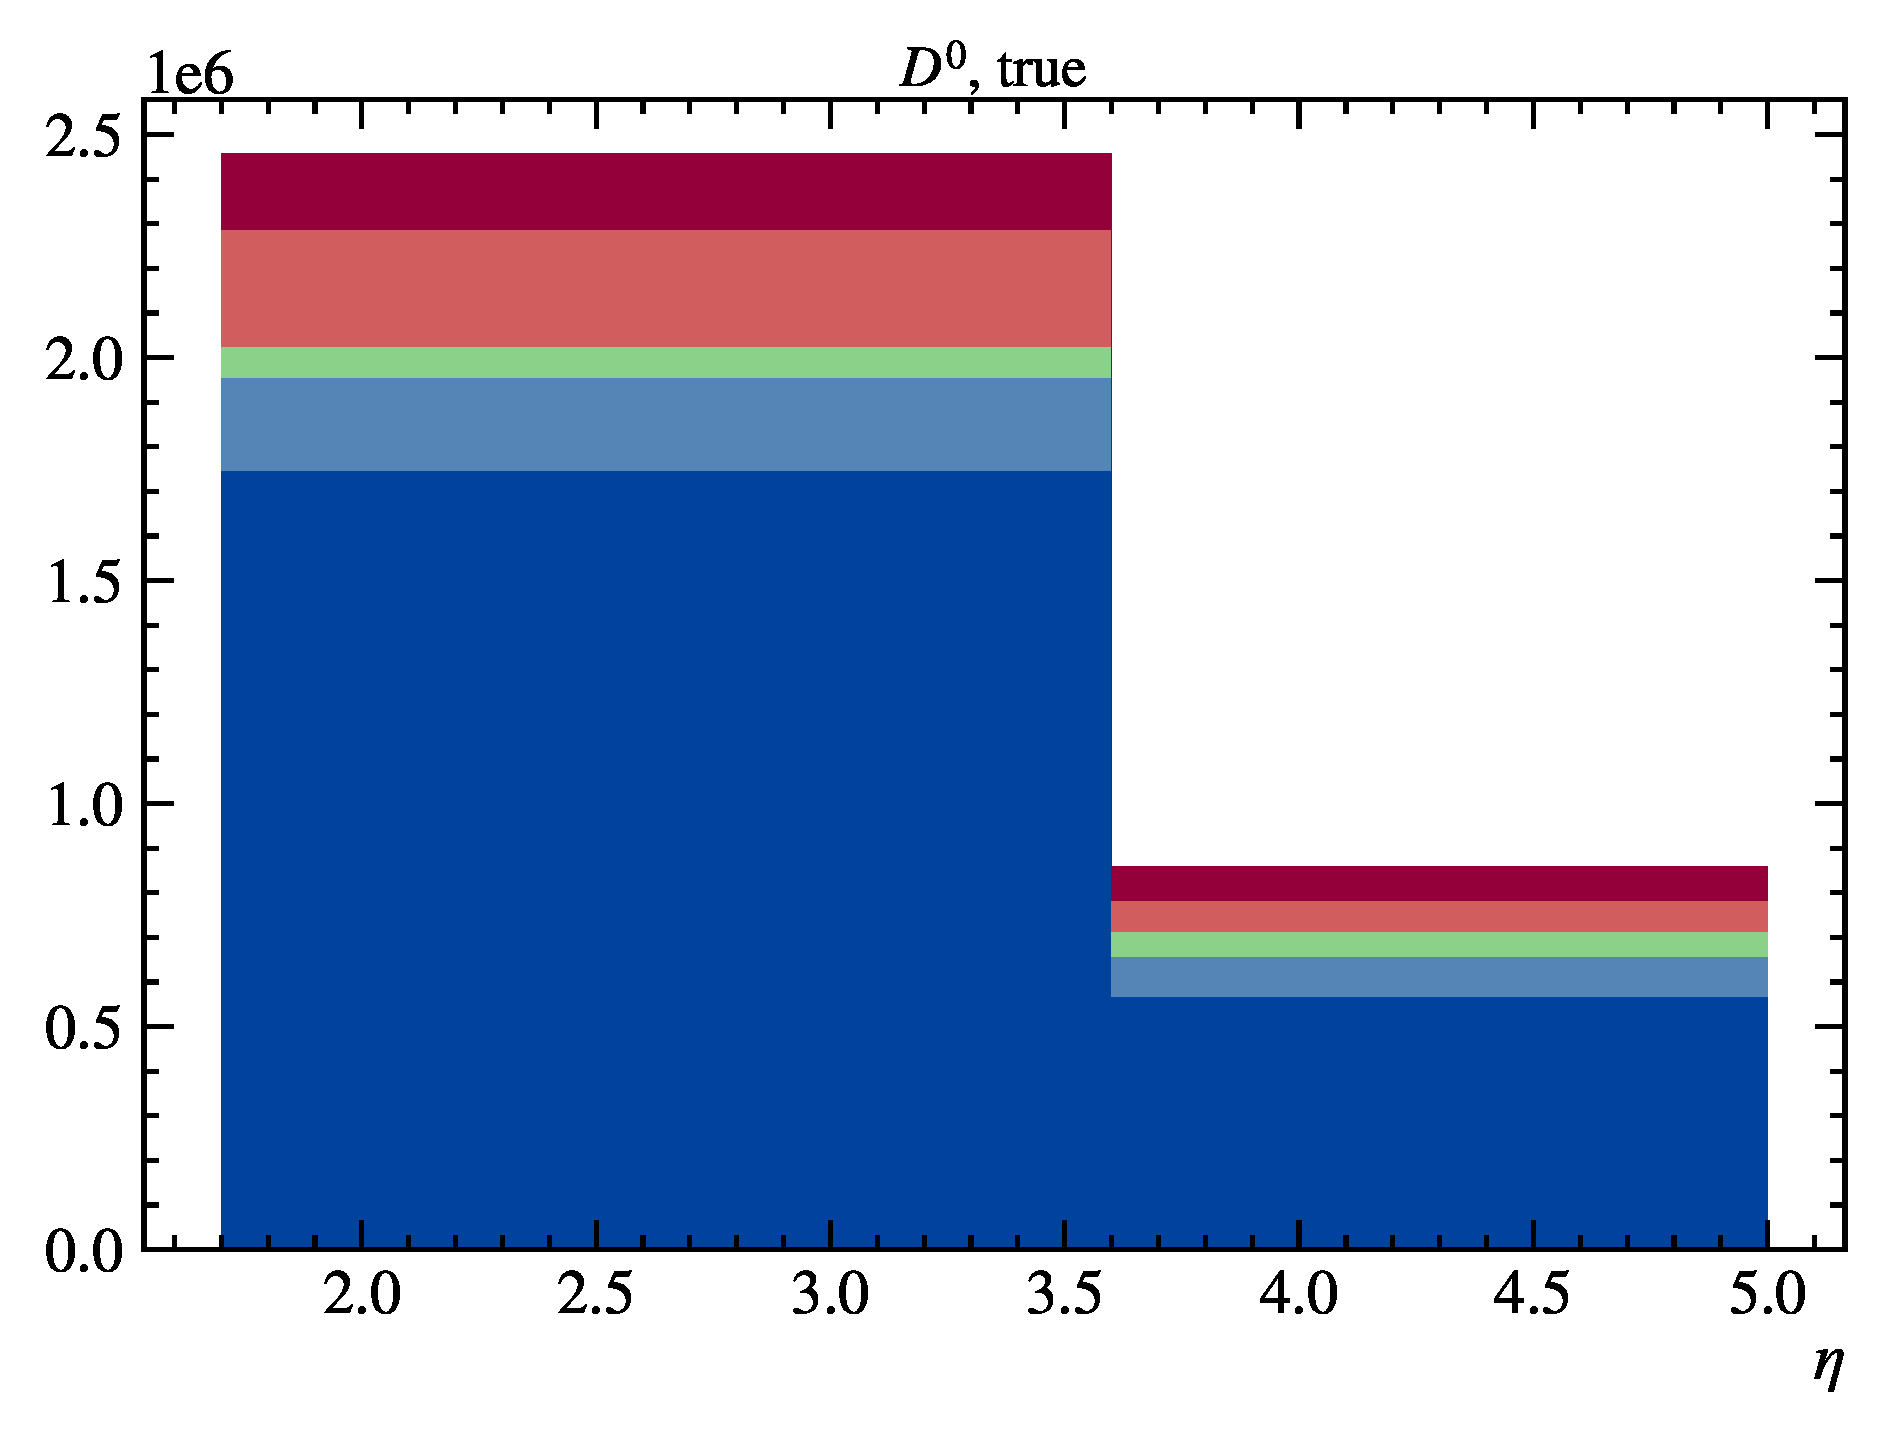
\includegraphics[width=\textwidth]{figs-fit-fit-templates/data-driven-plots/misid/D0-true_eta.pdf}
    \end{subfigure}
    \hfill
    \begin{subfigure}[b]{0.32\textwidth}
        \centering
        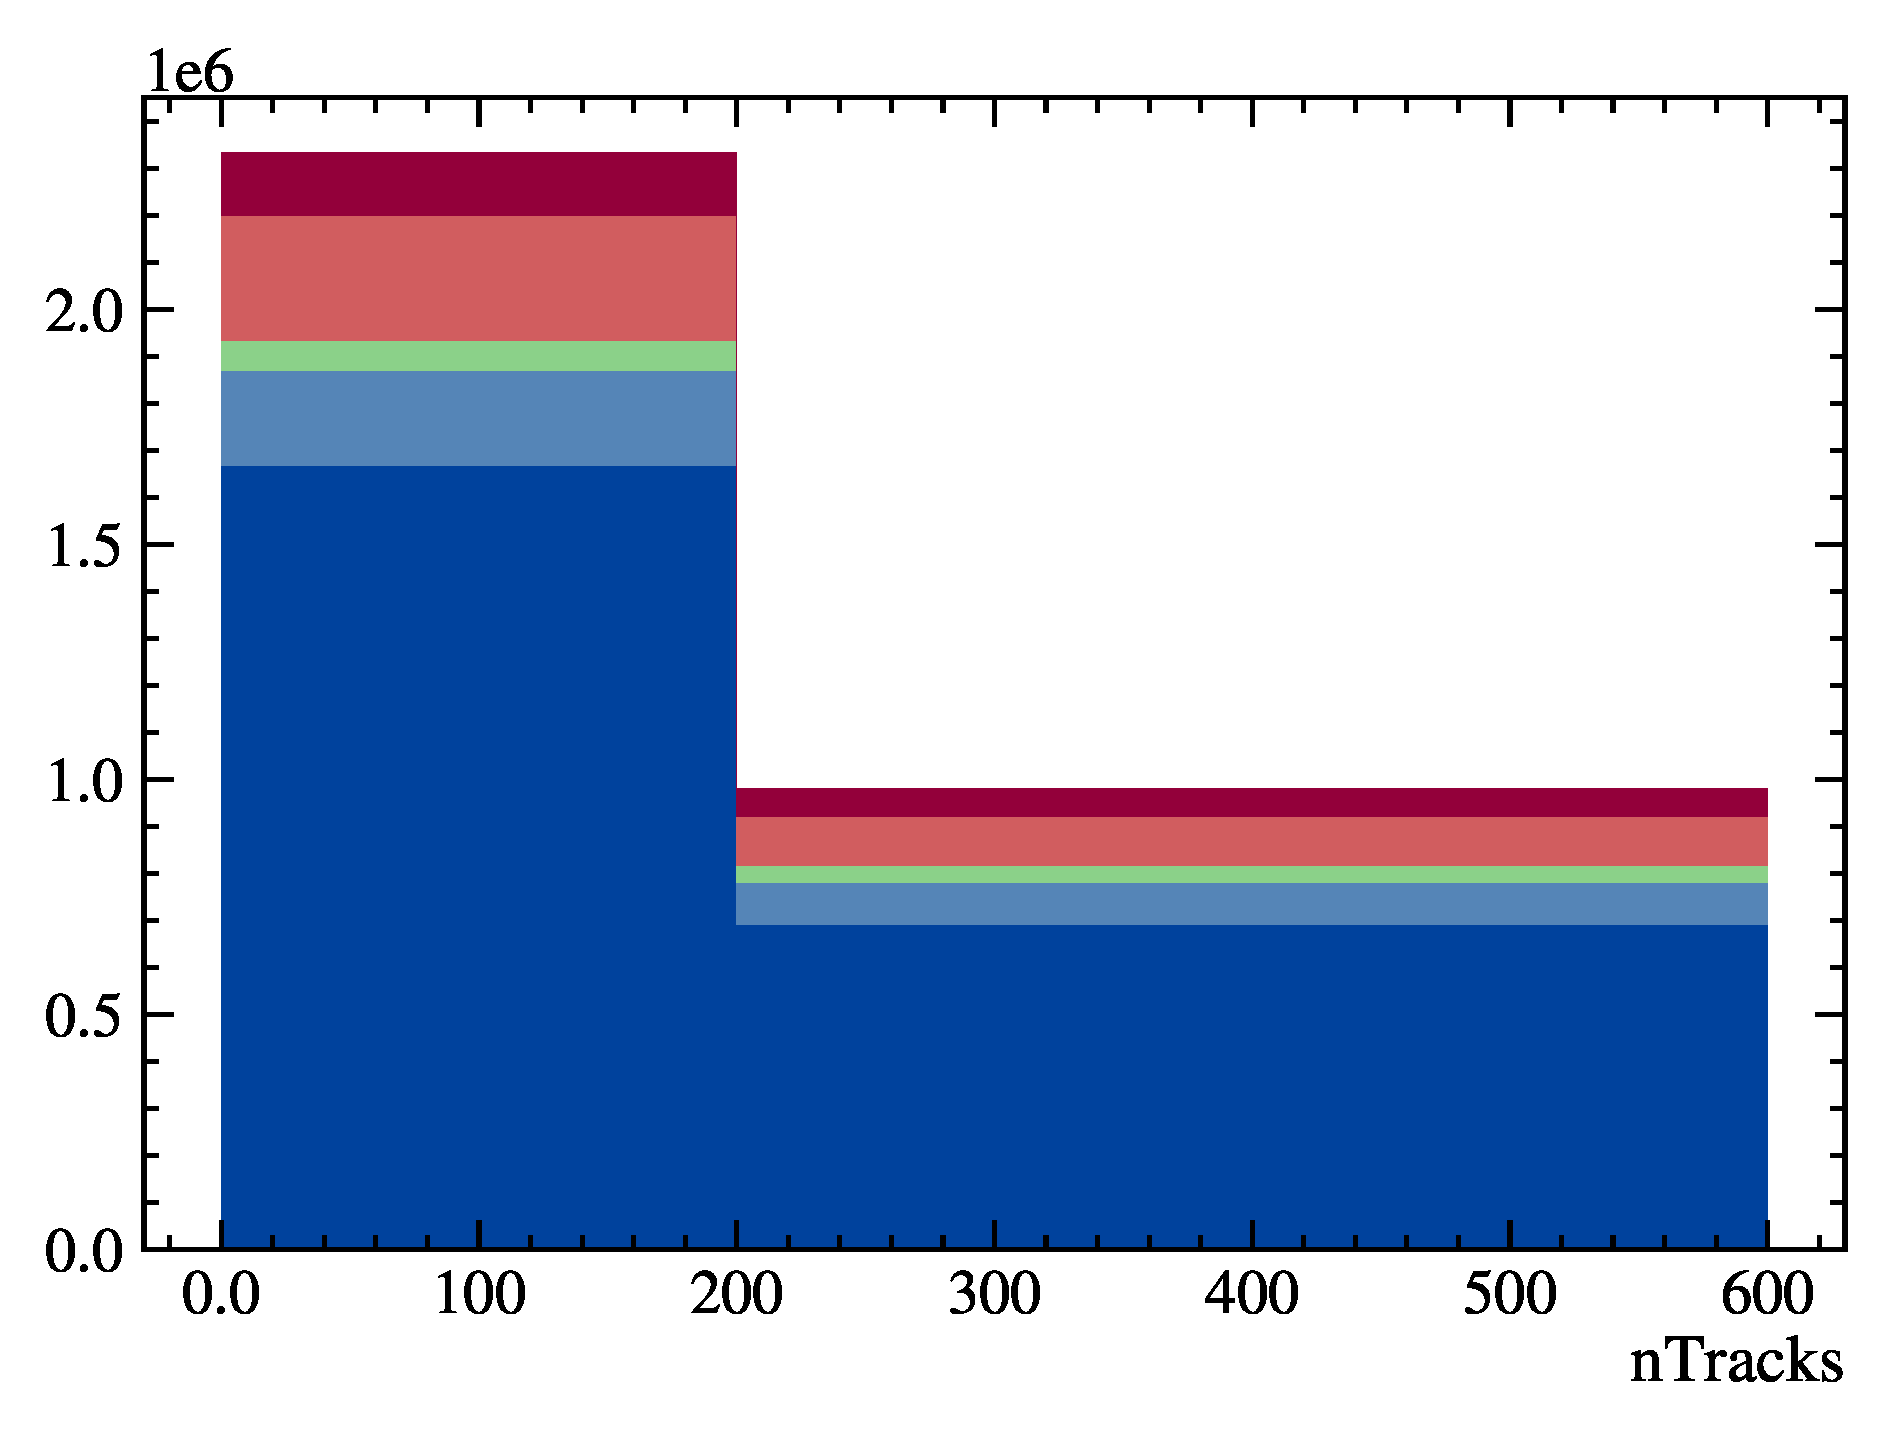
\includegraphics[width=\textwidth]{figs-fit-fit-templates/data-driven-plots/misid/D0-true_ntracks.pdf}
    \end{subfigure}
    \caption[misID tagged vs. unfolded.]{
        Unfolding effect displayed in $p$ and $\eta$ of the fake $\mu$ track,
        and nTracks of the reconstructed event.
        Top are the raw tagged yields,
        bottom are the unfolded true yields.
        The number of events is conserved by unfolding.

        The samples displayed here are 2016 $D^0$ fake \muon control samples
        $B^- \rightarrow D^0 t^-$ passing selections listed in
        \cref{ref:sel:data:fake-mu}.
    }
    \label{fig:unfolding-binning-vars}
\end{figure}

% Generated in /lhcb-ntuples-gen/studies/plot-RDX_misid_unfold_fit_vars, by
% running the script gen.sh inside
\begin{figure}[!htb]
    \centering
    \begin{subfigure}[b]{0.32\textwidth}
        \centering
        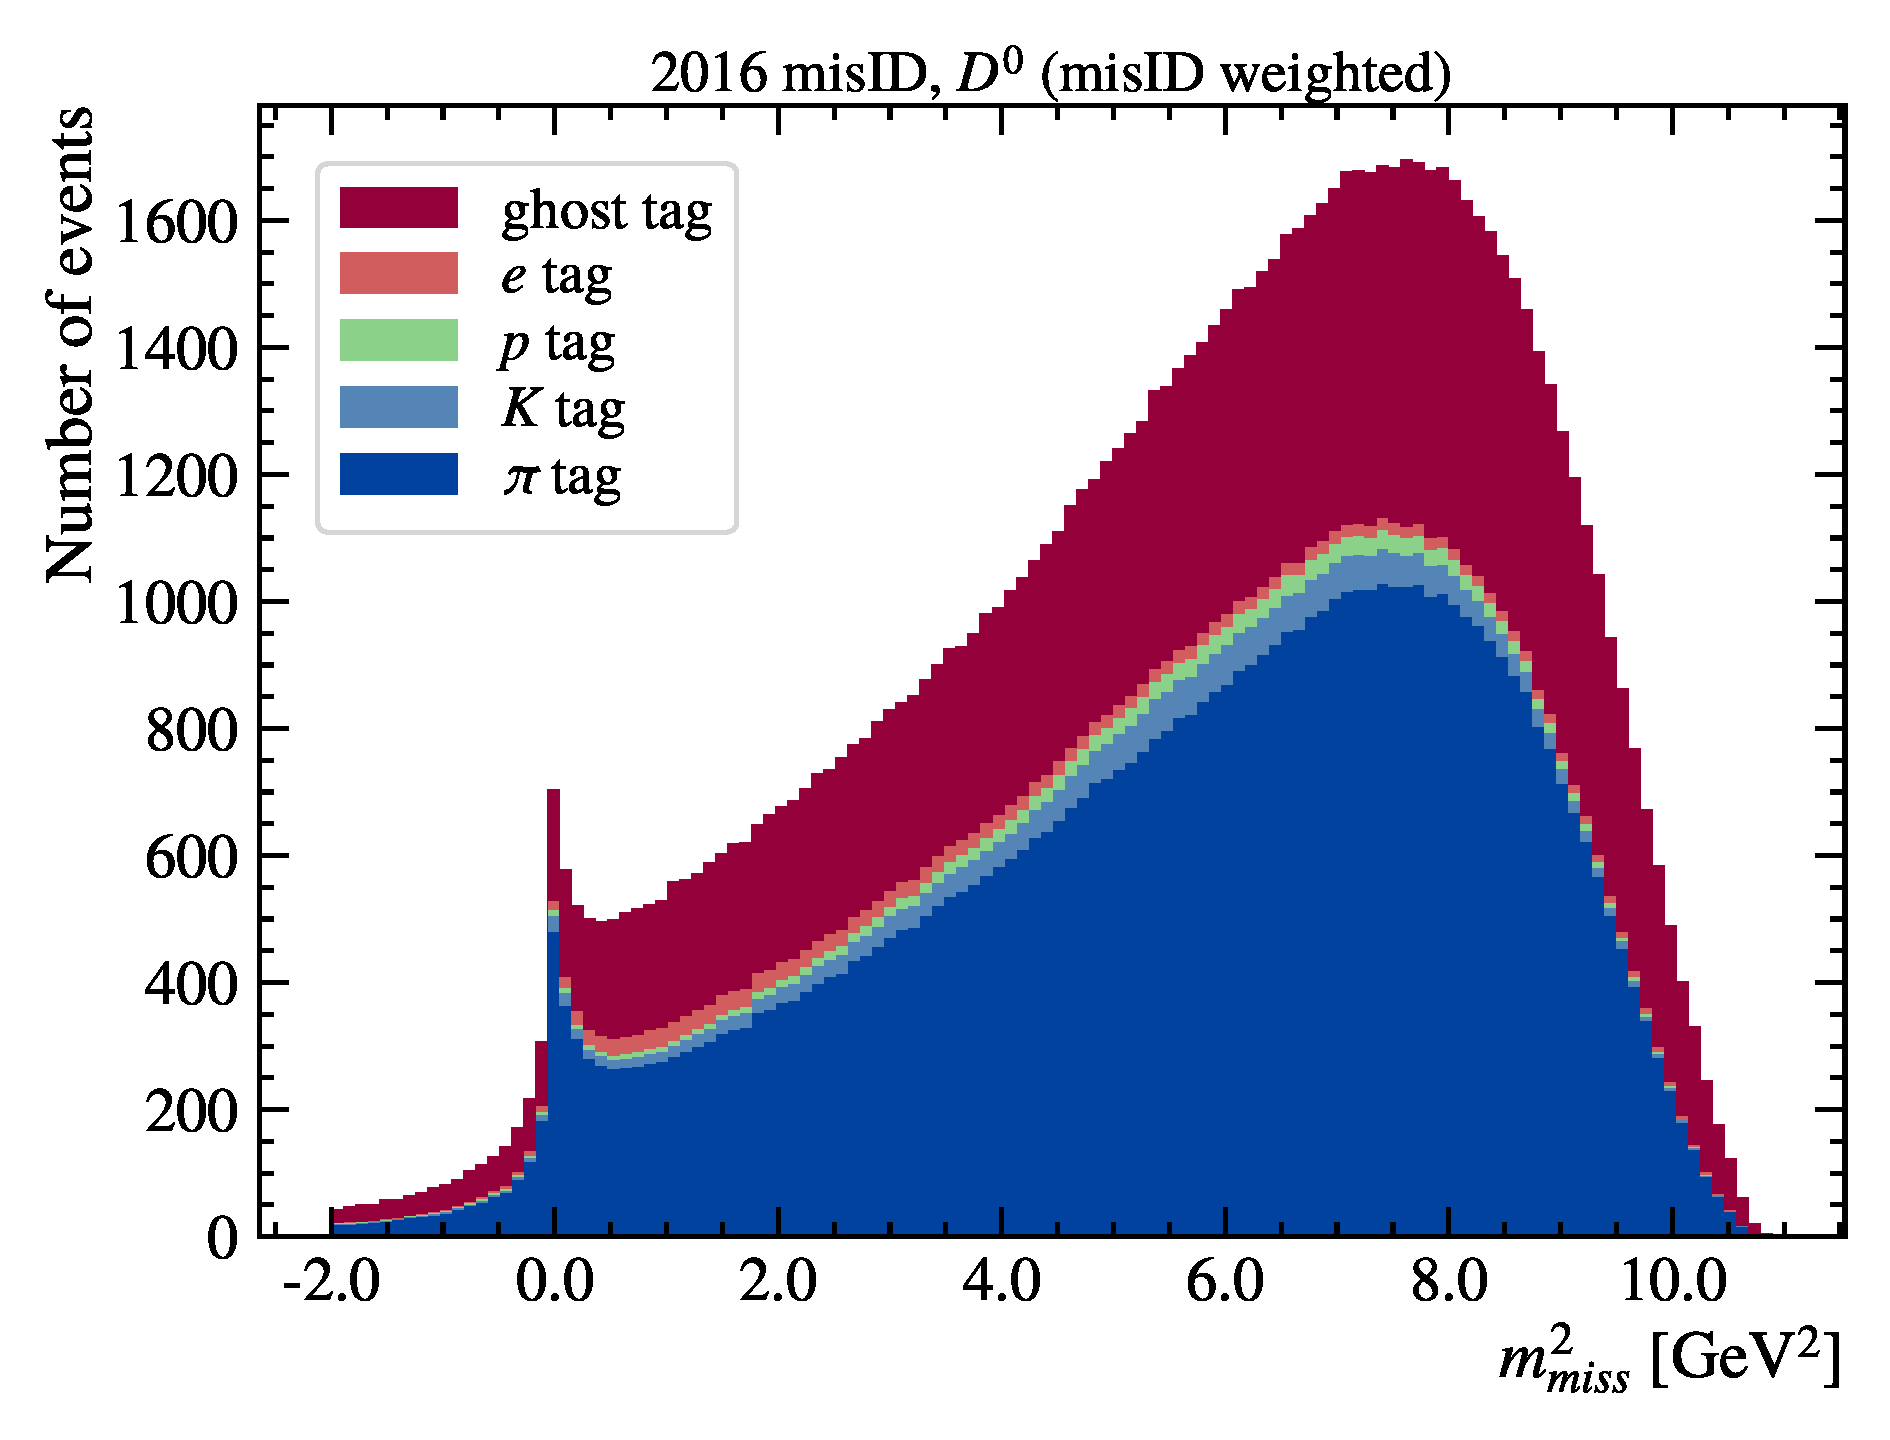
\includegraphics[width=\textwidth]{figs-fit-fit-templates/data-driven-plots/misid/D0_mm2.pdf}
    \end{subfigure}
    \hfill
    \begin{subfigure}[b]{0.32\textwidth}
        \centering
        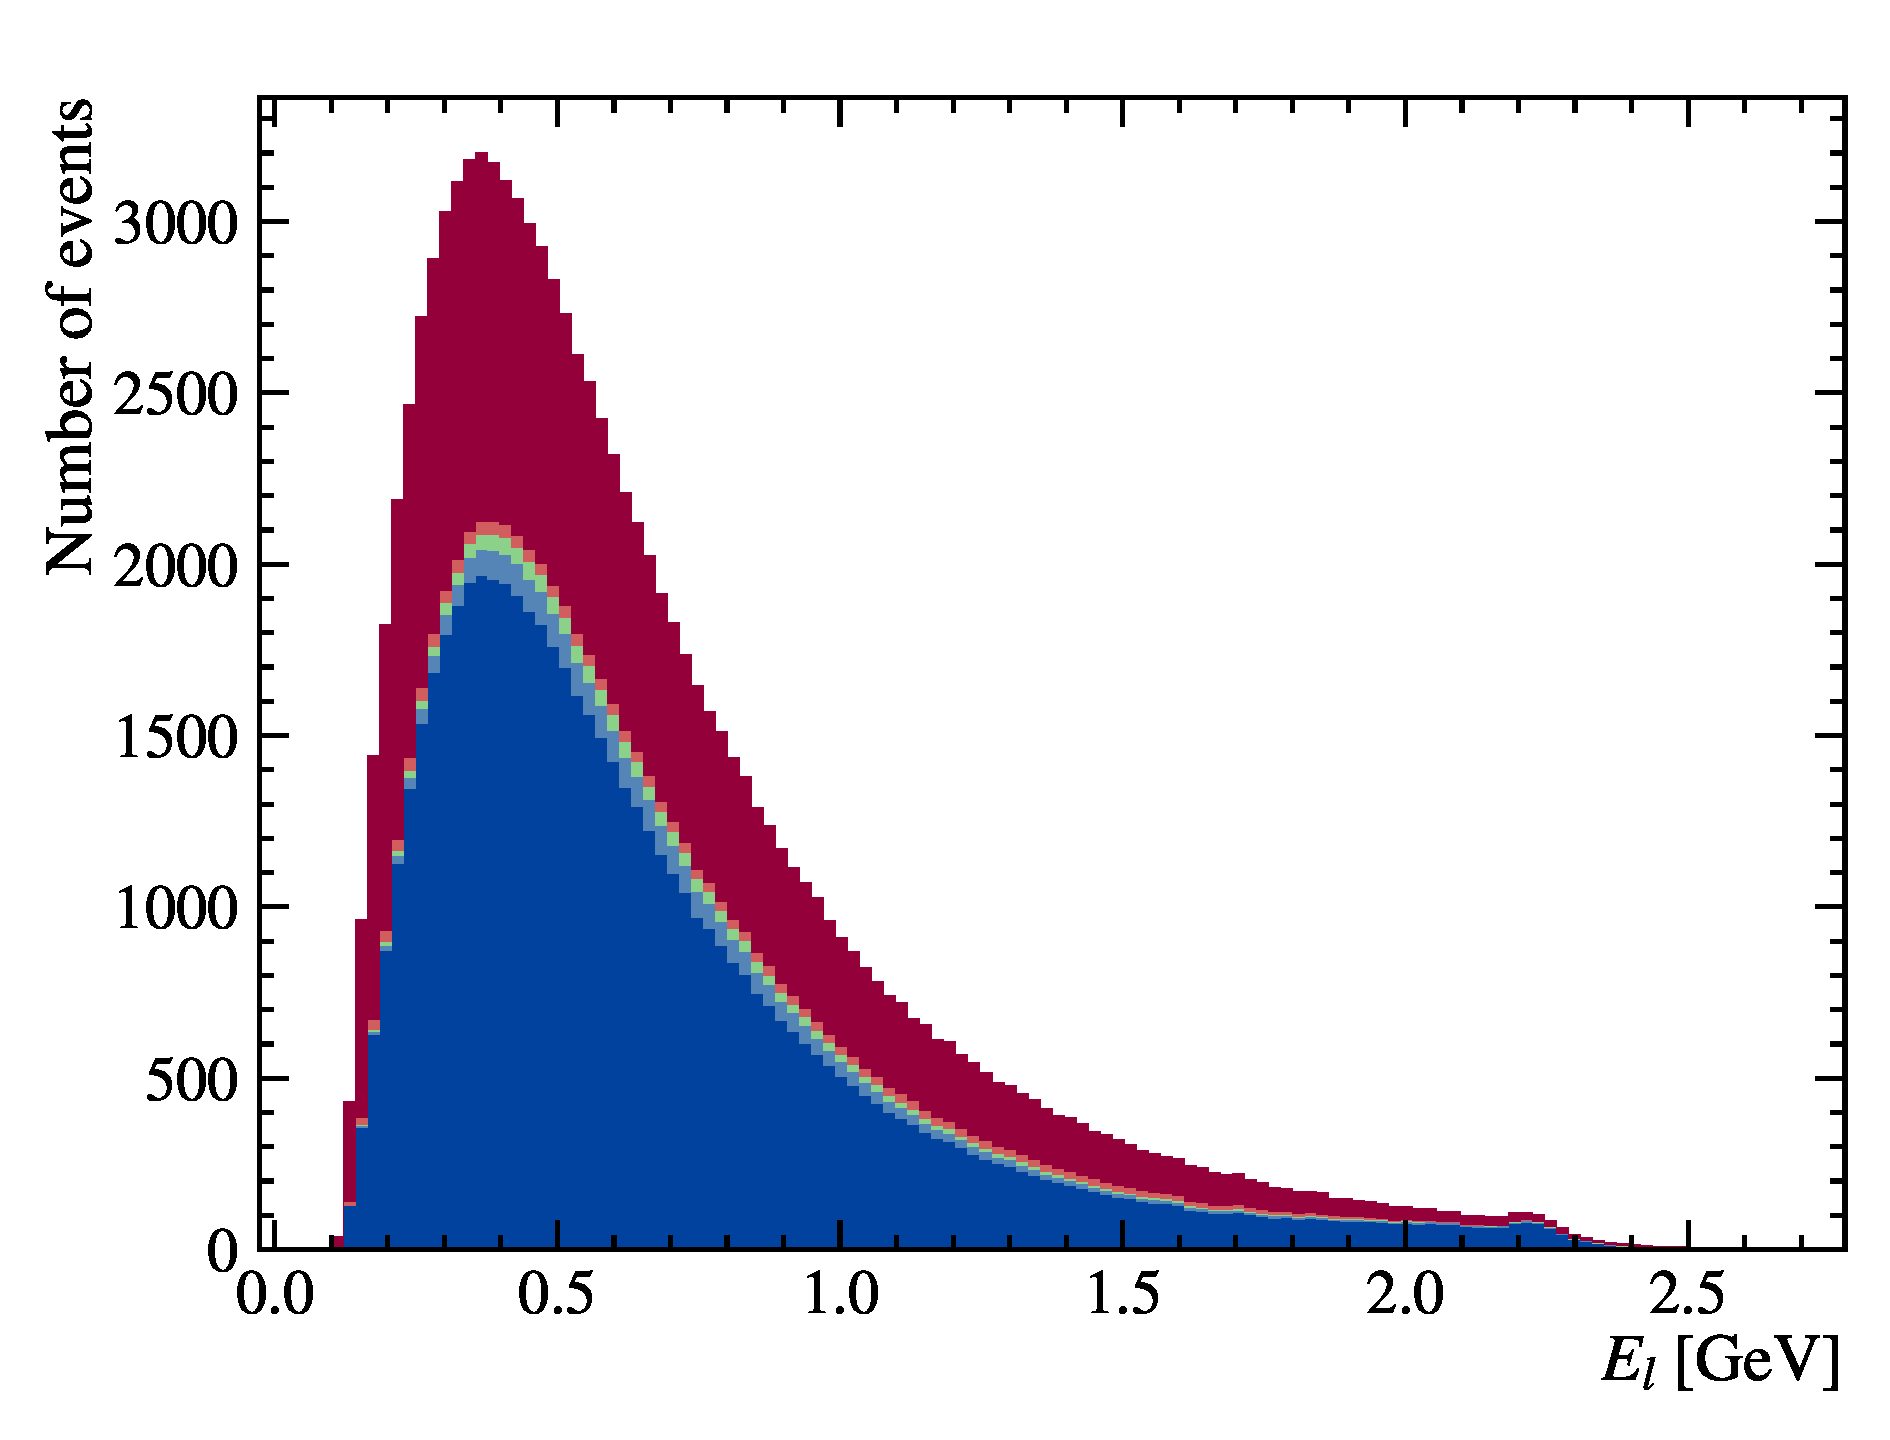
\includegraphics[width=\textwidth]{figs-fit-fit-templates/data-driven-plots/misid/D0_el}
    \end{subfigure}
    \hfill
    \begin{subfigure}[b]{0.32\textwidth}
        \centering
        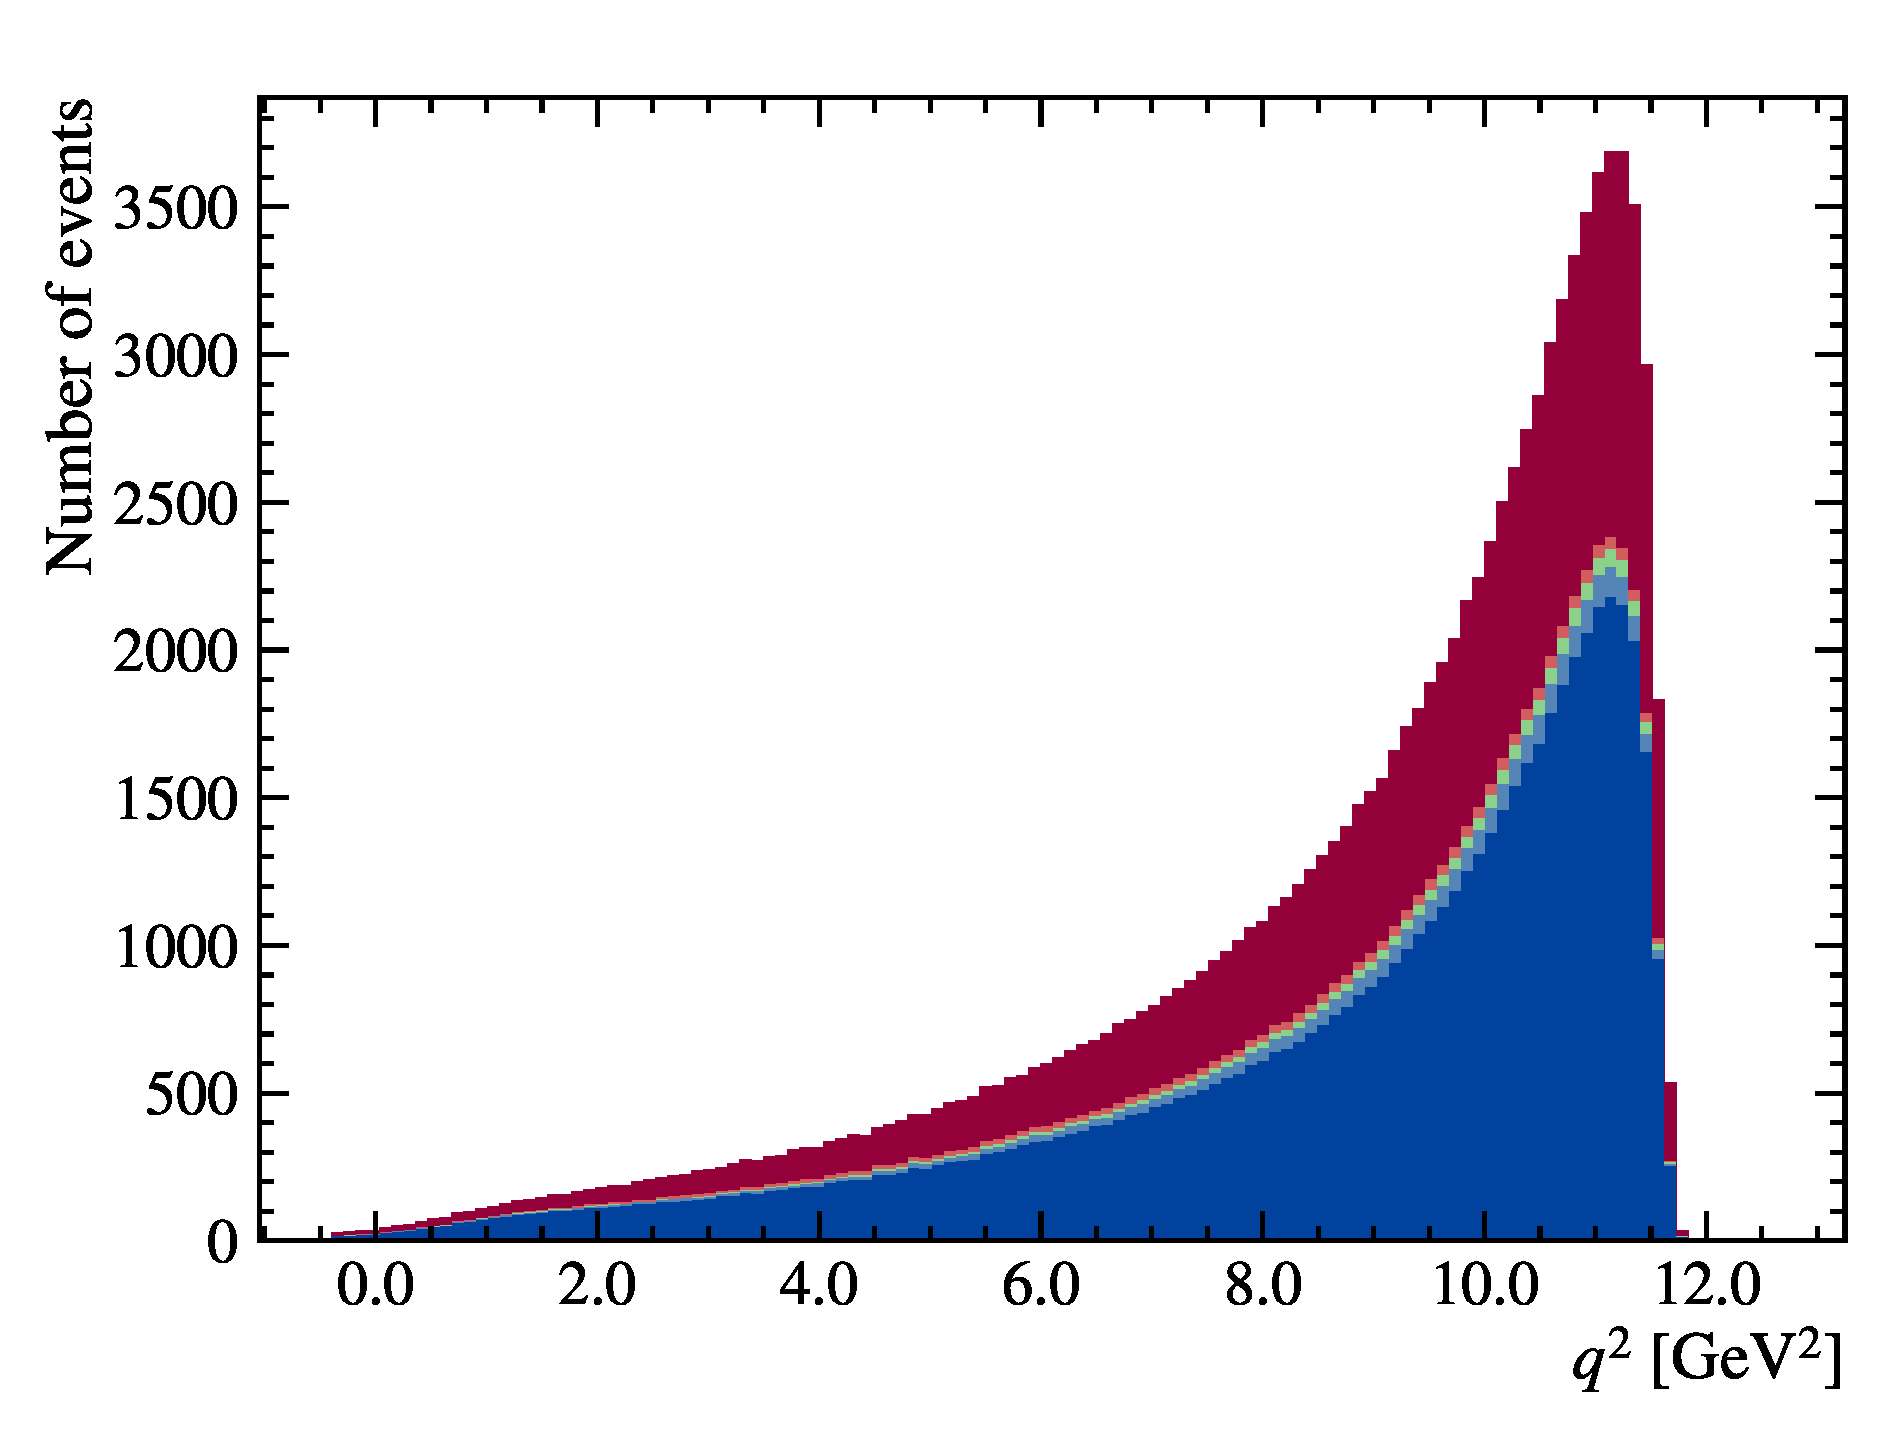
\includegraphics[width=\textwidth]{figs-fit-fit-templates/data-driven-plots/misid/D0_q2.pdf}
    \end{subfigure}
    \caption[Weighted yields of fake \muon sample.]{
        The weighted yields of each species of fake \muon sample projected in
        fit variables.
        The dominate contributions to the ``real'' muon samples are from
        \pion-like and ghost-like tracks.
        The binning are finer compared to \cref{fig:misid-vs-sig}. Actual
        yields are displayed without any rescaling.
    }
    \label{fig:unfolding-fit-vars}
\end{figure}

\begin{table}[!htb]
    \centering
    \caption{Selections for each tagged species in fake \muon sample.}
    \label{tab:selection-for-tagged-species}
    \begin{tabular}{crl}
        \toprule
        {\bf Tagged species} & {\bf Variable}            & {\bf Selection} \\
        \midrule
        $\pi$                & \ProbNN{\pion}            & $> 0.1$   \\
                             & \PID{\kaon}               & $< 0.0$   \\
                             & \PID{$p$}                 & $< 0.0$   \\
                             & \PID{$e$}                 & $< 2.0$   \\
                             & \ProbNN{ghost}            & $< 0.25$  \\
        \midrule
        $K$                  & \ProbNN{\kaon}            & $> 0.1$   \\
                             & \PID{\kaon}               & $> 0.0$   \\
                             & \PID{$p$} $-$ \PID{\kaon} & $< 0.0$   \\
                             & \PID{$e$} $-$ \PID{\kaon} & $< -2.0$  \\
                             & \ProbNN{ghost}            & $< 0.25$  \\
        \midrule
        $p$                  & \ProbNN{$p$}              & $> 0.1$   \\
                             & \PID{$p$}                 & $> 0.0$   \\
                             & \PID{$p$} $-$ \PID{\kaon} & $> 2.0$   \\
                             & \PID{$e$} $-$ \PID{$p$}   & $< -2.0$  \\
                             & \ProbNN{ghost}            & $< 0.25$  \\
        \midrule
        $e$                  & \PID{$e$}                 & $> 2.0$   \\
                             & \PID{$e$} $-$ \PID{\kaon} & $> -2.0$  \\
                             & \PID{$e$} $-$ \PID{$p$}   & $> -2.0$  \\
                             & \ProbNN{ghost}            & $< 0.25$  \\
        \midrule
        ghost                & Not in any species above  & \\
        \bottomrule
    \end{tabular}
\end{table}


\subsection{Combinatorial backgrounds}
\label{ref:fit:tmpl:comb}

The selection procedures for all combinatorial backgrounds are listed
in \cref{ref:sel:data:ws}.
The generation procedure for these templates is documented below.
A comparison between combinatorial backgrounds and signal templates is
shown in \cref{fig:comb-vs-sig}.

% TODO: Implement comb. bkg. tmpl. comparison
\begin{figure}[!htb]
    \centering
    \begin{subfigure}[t]{0.9\textwidth}
        \centering
        \caption{
            \BComb and \DstComb vs. $\Bm \rightarrow \Dz\taum\neutb$ in \Dz channel.
        }
    \end{subfigure}

    \begin{subfigure}[t]{0.9\textwidth}
        \centering
        \caption{
            \BComb vs. $\Bzb \rightarrow \Dstarp\taum\neutb$ in \Dstar channel.
        }
    \end{subfigure}

    \caption{
        Comparison between combinatorial backgrounds and signal template.
    }
    \label{fig:comb-vs-sig}
\end{figure}

\subsubsection{$D^*$ combinatorial}
\label{dst-comb}

The $D^*$ combinatorial background (\DstComb) arises from a reconstructed $D^0$
combining with an random slow $\pi$, forming a fake $D^*$ vertex and
passing all selection requirements.

The shape of \DstComb can be determined from wrong-sign $\pi$ (WS $\pi$) control
sample which contains mostly $D^0 \pi^-$ pairs.
Still, the yields of \DstComb between nominal right-sign (RS) sample and
WS $\pi$ are not the same,
likely due to differences in selection efficiencies.
Thus a fit on the RS sample is performed to obtain
the yield of \DstComb, then the WS $\pi$ is rescaled to match the fitted yield.
The fit procedure is the following:

\begin{enumerate}
    \item Remove misID contribution from RS sample.
    \item Remove misID contribution from WS $\pi$ sample\footnote{
            A WS $\pi$ control sample from misID sample is reconstructed to
            obtain the misID contribution for data WS $\pi$.
        }.
    \item Fit the mass window $m_{D^*} - m_{D^0}$ (including events normally
        outside the window) on RS sample with a
        double-Gaussian signal and an exponential background.
        The background yield under the mass window where a $D^*$ is nominally
        accepted is taken as the yield of \DstComb.

        The fit to ISO skim is shown in \cref{fig:dst-comb-fit}.
        The effect of scaling for the ISO skim is shown in
        \cref{fig:dst-comb-scale}.
        For fit to 1OS, 2OS, and DD skims, refer to \cref{appx:suppl:dst-comb}.
\end{enumerate}

\techlink{appx:tech:fit-to-comb-bkg}

% Generated in /rdx-run2-analysis/fit with the command:
%   make fit-DstComb
\begin{figure}[!htb]
    \centering
    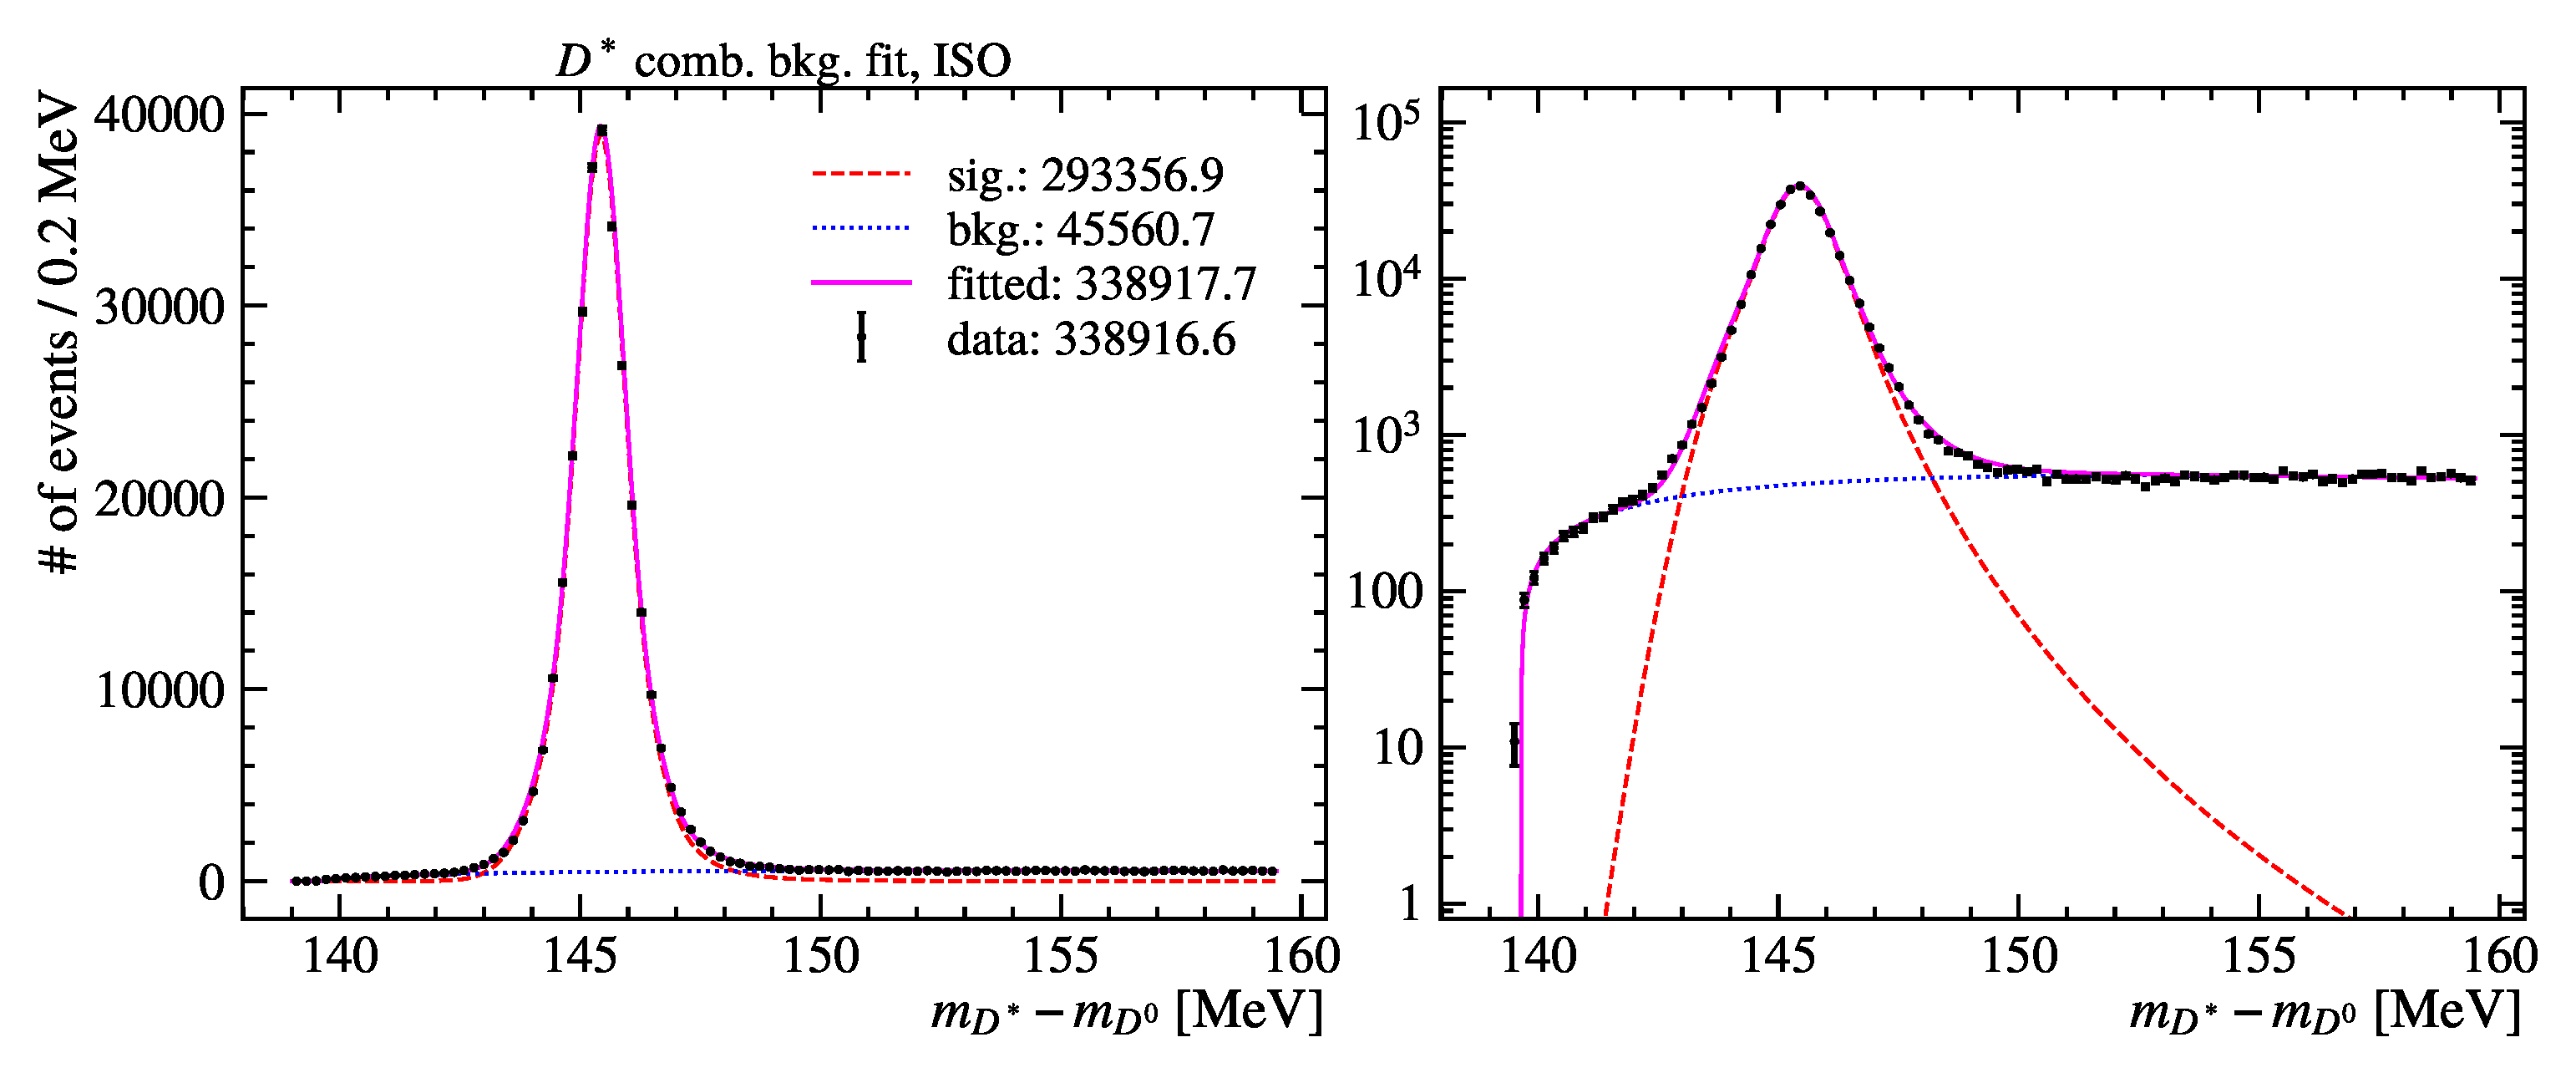
\includegraphics[width=\textwidth]{figs-fit-fit-templates/data-driven-plots/dst_comb/fit_dst_comb_iso_comb.pdf}
    \caption{
        \DstComb\ auxiliary fit to the ISO skim.
        Right plot shows the same fit as in the left, but with a logarithmic $y$
        axis.
    }
    \label{fig:dst-comb-fit}
\end{figure}

\begin{figure}[!htb]
    \centering
    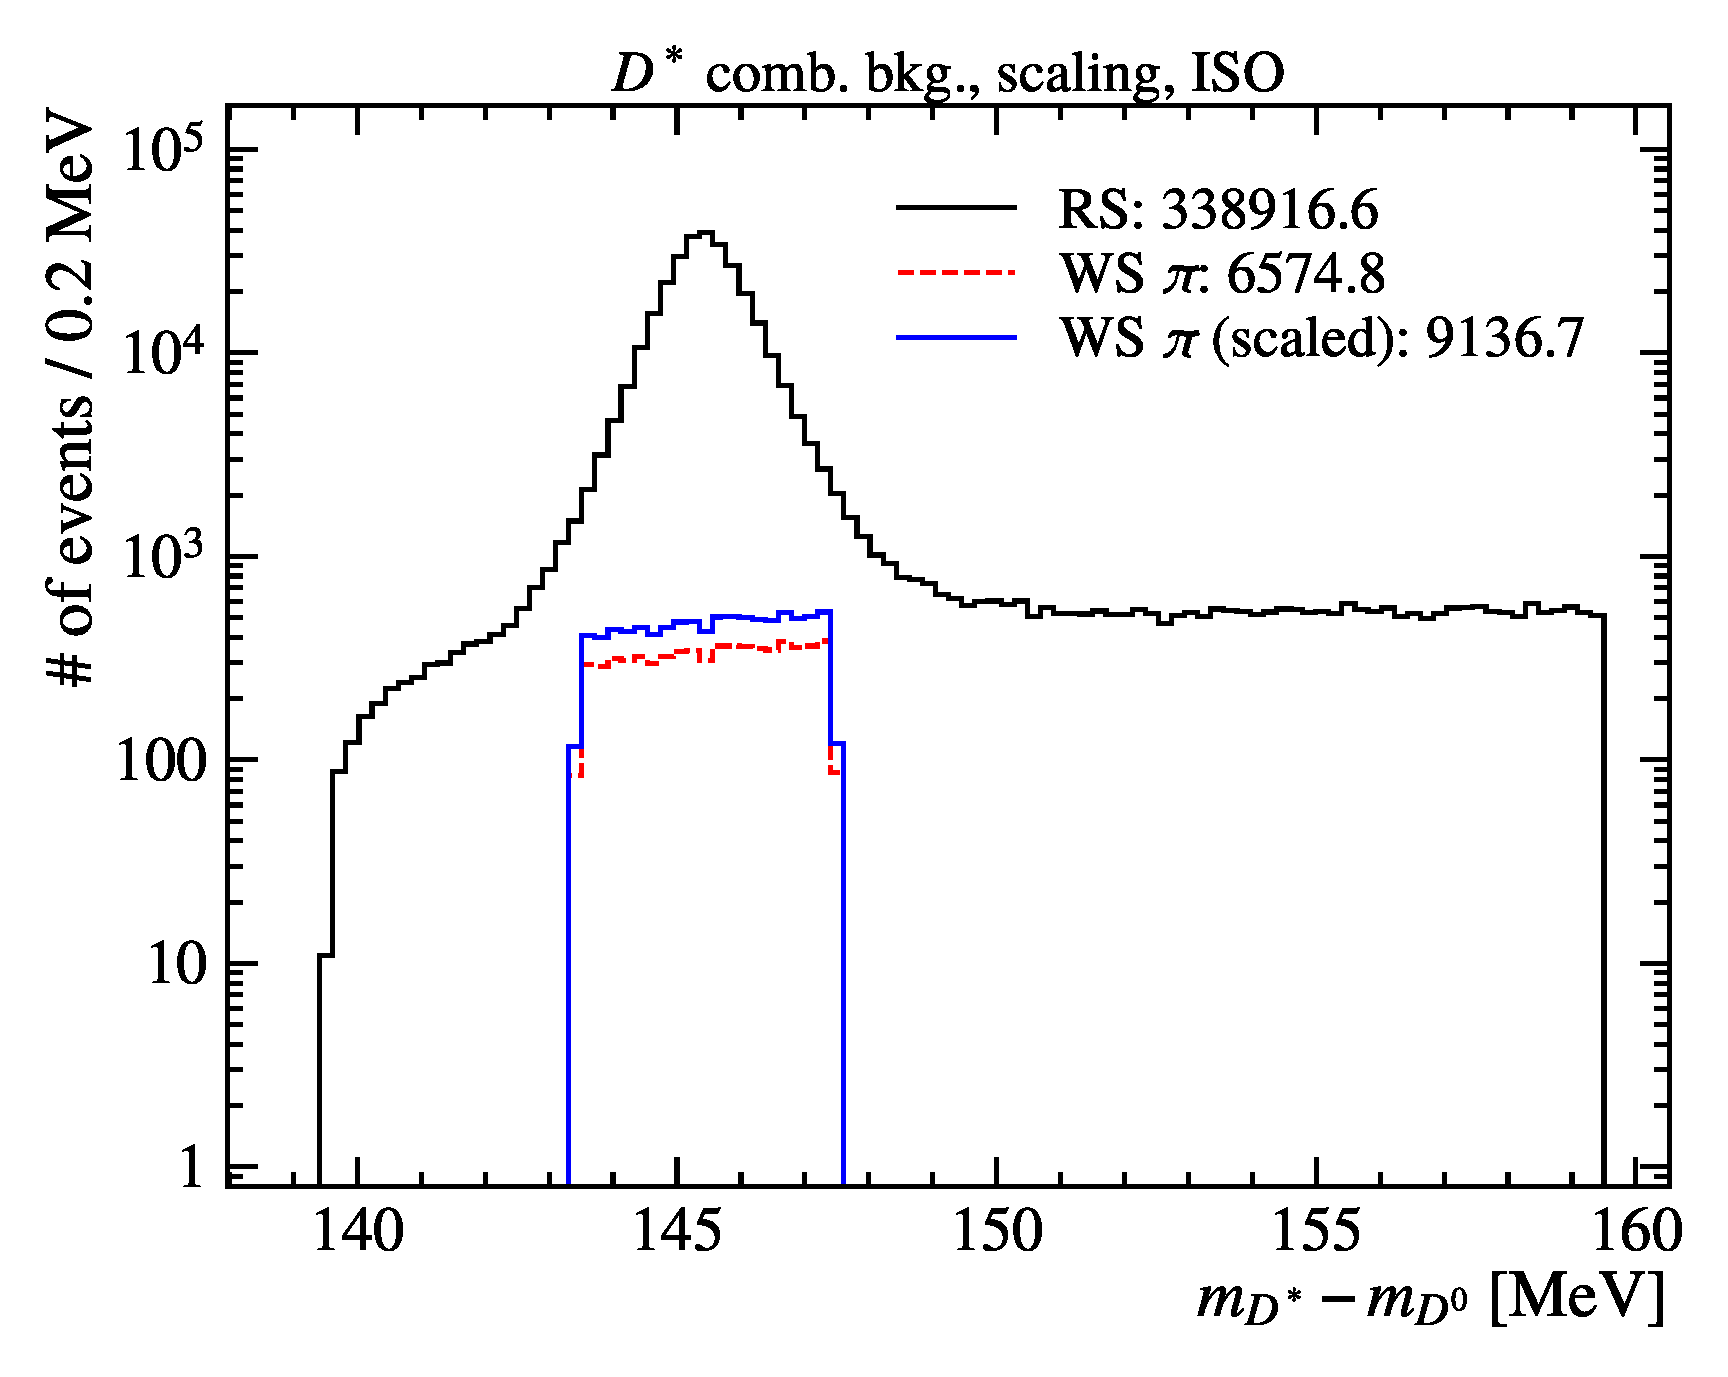
\includegraphics[width=0.55\textwidth]{figs-fit-fit-templates/data-driven-plots/dst_comb/fit_dst_comb_scaled_comp_iso_log.pdf}
    \caption{
        Effect of scaling for the ISO skim on the \DstComb\ template.
    }
    \label{fig:dst-comb-scale}
\end{figure}

\subsubsection{$B$ combinatorial in $D^*$ channel}
\label{b-comb-dst}

The $B$ combinatorial (\BComb) in $D^*$ fit channel comes from randomly
combined $D^* \mu$ pairs.
Again, the shape of the \BComb\ is determined by wrong-sign $\mu$ (WS $\mu$)
control sample containing $D^{*+} \mu^+$ pairs.

Further, it is assumed that the \BComb\ from WS $\mu$ and \BComb\ from RS
differs by a factor linear in $m_B$.
This is justified by assuming \BComb\ are slow-varying exponential decays in
terms of $m_B$ for both RS and WS $\mu$, thus the ratio between the two is also
an exponential.
Since they are slow-varying, Taylor expansion to the first order (i.e. of the
form $a + b m_B$) agrees well with the ratio in a sufficiently large region.

Unlike $m_\Dstar$ in \DstComb,
$m_B$ does not have a clear lower side-band.
This is because \B is only \emph{partially} reconstructed
due to missing neutrino(s).
Therefore, only the upper-sideband, defined as $m_B > 5400$ MeV,
which contains purely combinatorial and misID, can be used to
study \BComb.

A fit is performed in $B$ mass upper-sideband  to obtain
the linear scaling factor $a + b m_B$.
In the upper-sideband, it is assumed that both WS $\mu$ and RS samples contain
are pure, that is, containing only combinatorial backgrounds and misID.
The linear scaling factor is assumed to be the same for all skims\footnote{
    This is mainly because there is not enough number of events in the
    upper-sideband to perform fits skim-by-skim.
}.
The fit is performed in the following manner:

\begin{enumerate}
    \item Remove misID contribution from RS sample.
    \item Remove misID contribution from WS $\mu$ sample.
    \item Perform a fit on RS sample in the upper-sideband region to determine
        contribution from \DstComb, with procedure identical to that in
        \cref{dst-comb}.
        Then remove the fitted \DstComb.
    \item Fit and remove \DstComb\ from WS $\mu$ sample.
    \item Compute the ratio between RS and WS $\mu$, perform a fit to obtain
        the linear scaling factor.
        The fit,
        as well as the raw RS, raw WS \muon, and scaled WS \muon templates,
        is shown in \cref{fig:b-comb-dst}.
\end{enumerate}

% FIXME: Replace quad. fit w/ an exp. fit
% Generated in /rdx-run2-analysis/fit with the command:
%   make fit-BCombDst
\begin{figure}[!htb]
    \centering
    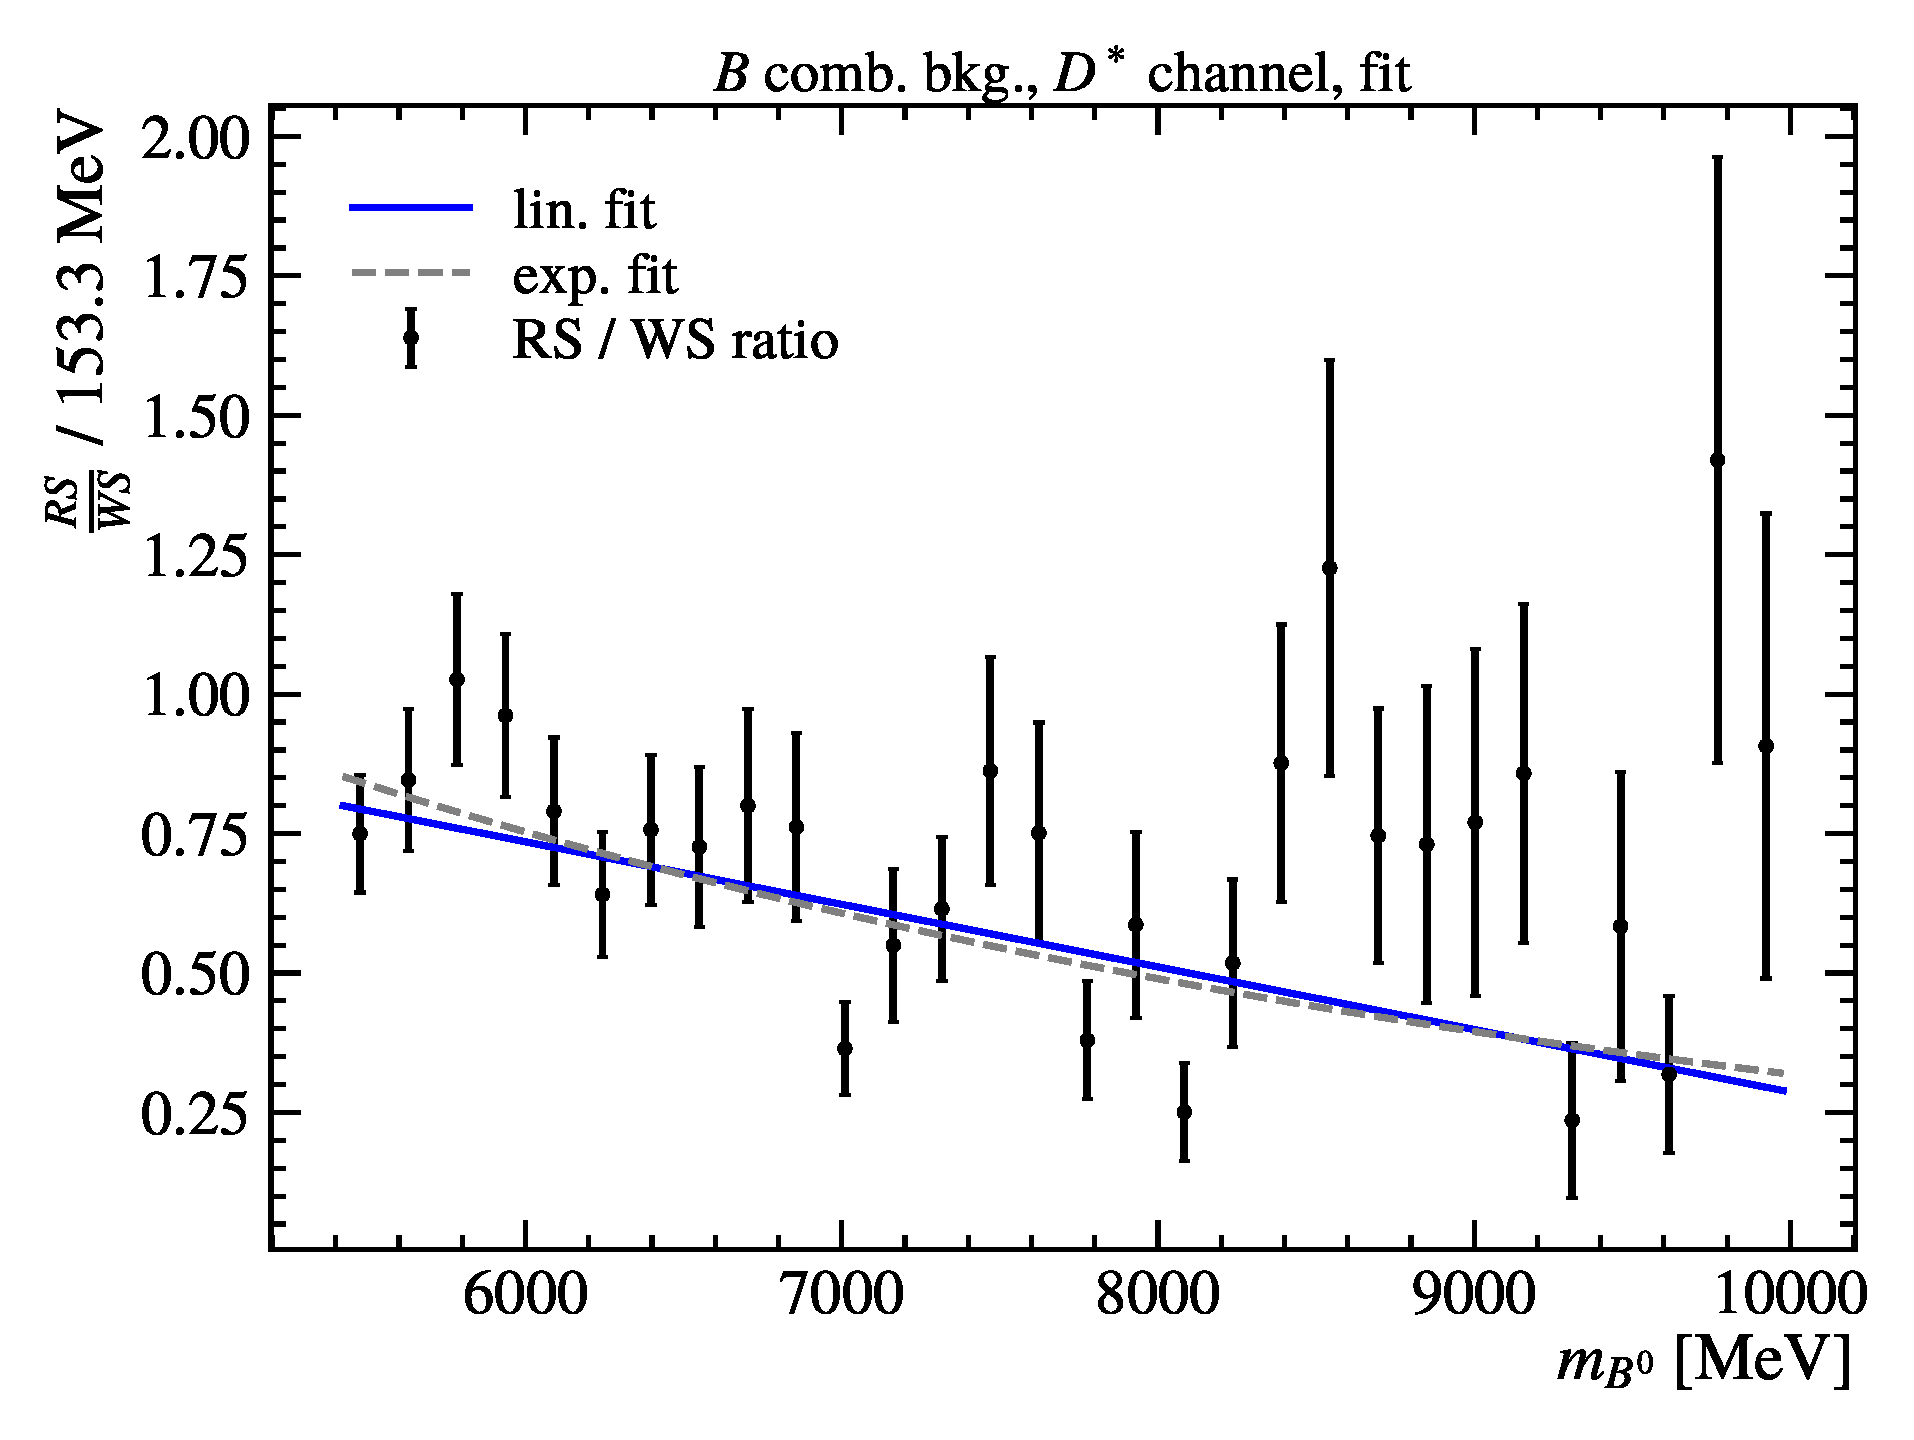
\includegraphics[width=0.48\textwidth]{figs-fit-fit-templates/data-driven-plots/b_comb/fit_b_comb_dst_fit.pdf}
    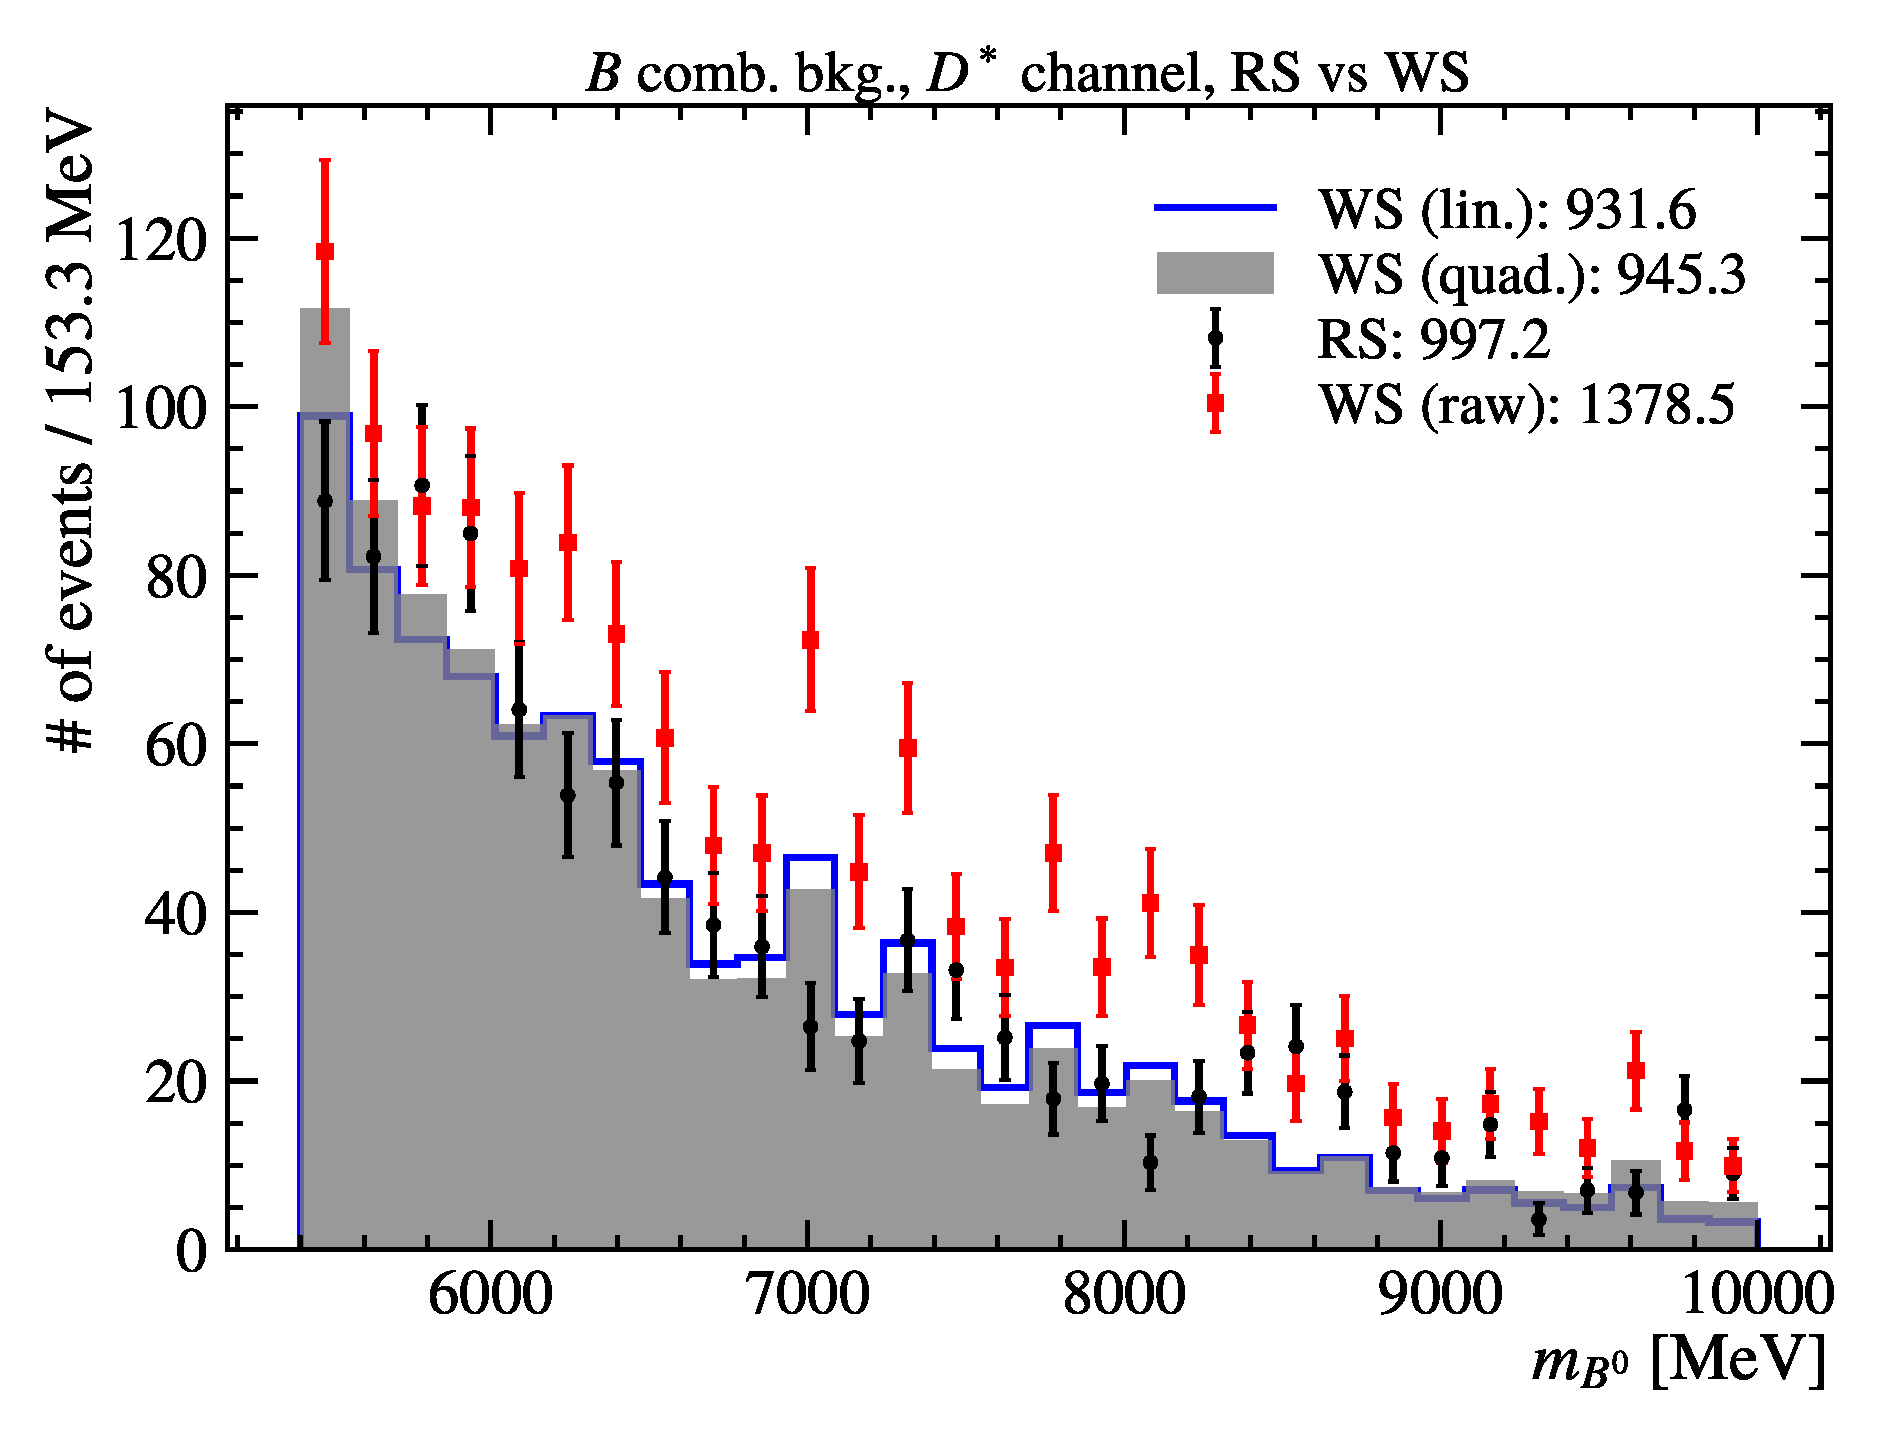
\includegraphics[width=0.48\textwidth]{figs-fit-fit-templates/data-driven-plots/b_comb/fit_b_comb_dst_scaled.pdf}

    \caption[\BComb\ fit result for $D^*$ channel]{
        \BComb\ fit result for $D^*$ channel.

        Left: \BComb\ auxiliary fit in the $m_B$ upper-sideband region for all skims.
        A quadratic fit is also performed for possible systematic studies.

        Right: The scaling effect on the WS $\mu$ \BComb\ template.
    }
    \label{fig:b-comb-dst}
\end{figure}

\subsubsection{$B$ combinatorial in $D^0$ channel}
\label{b-comb-d0}

The procedure is similar to that in \cref{b-comb-dst}, but without \DstComb\
removal. The fit is shown in \cref{fig:b-comb-d0}.

% FIXME: Replace quad. fit w/ an exp. fit
% Generated in /rdx-run2-analysis/fit with the command:
%   make fit-BCombD0
\begin{figure}[!htb]
    \centering
    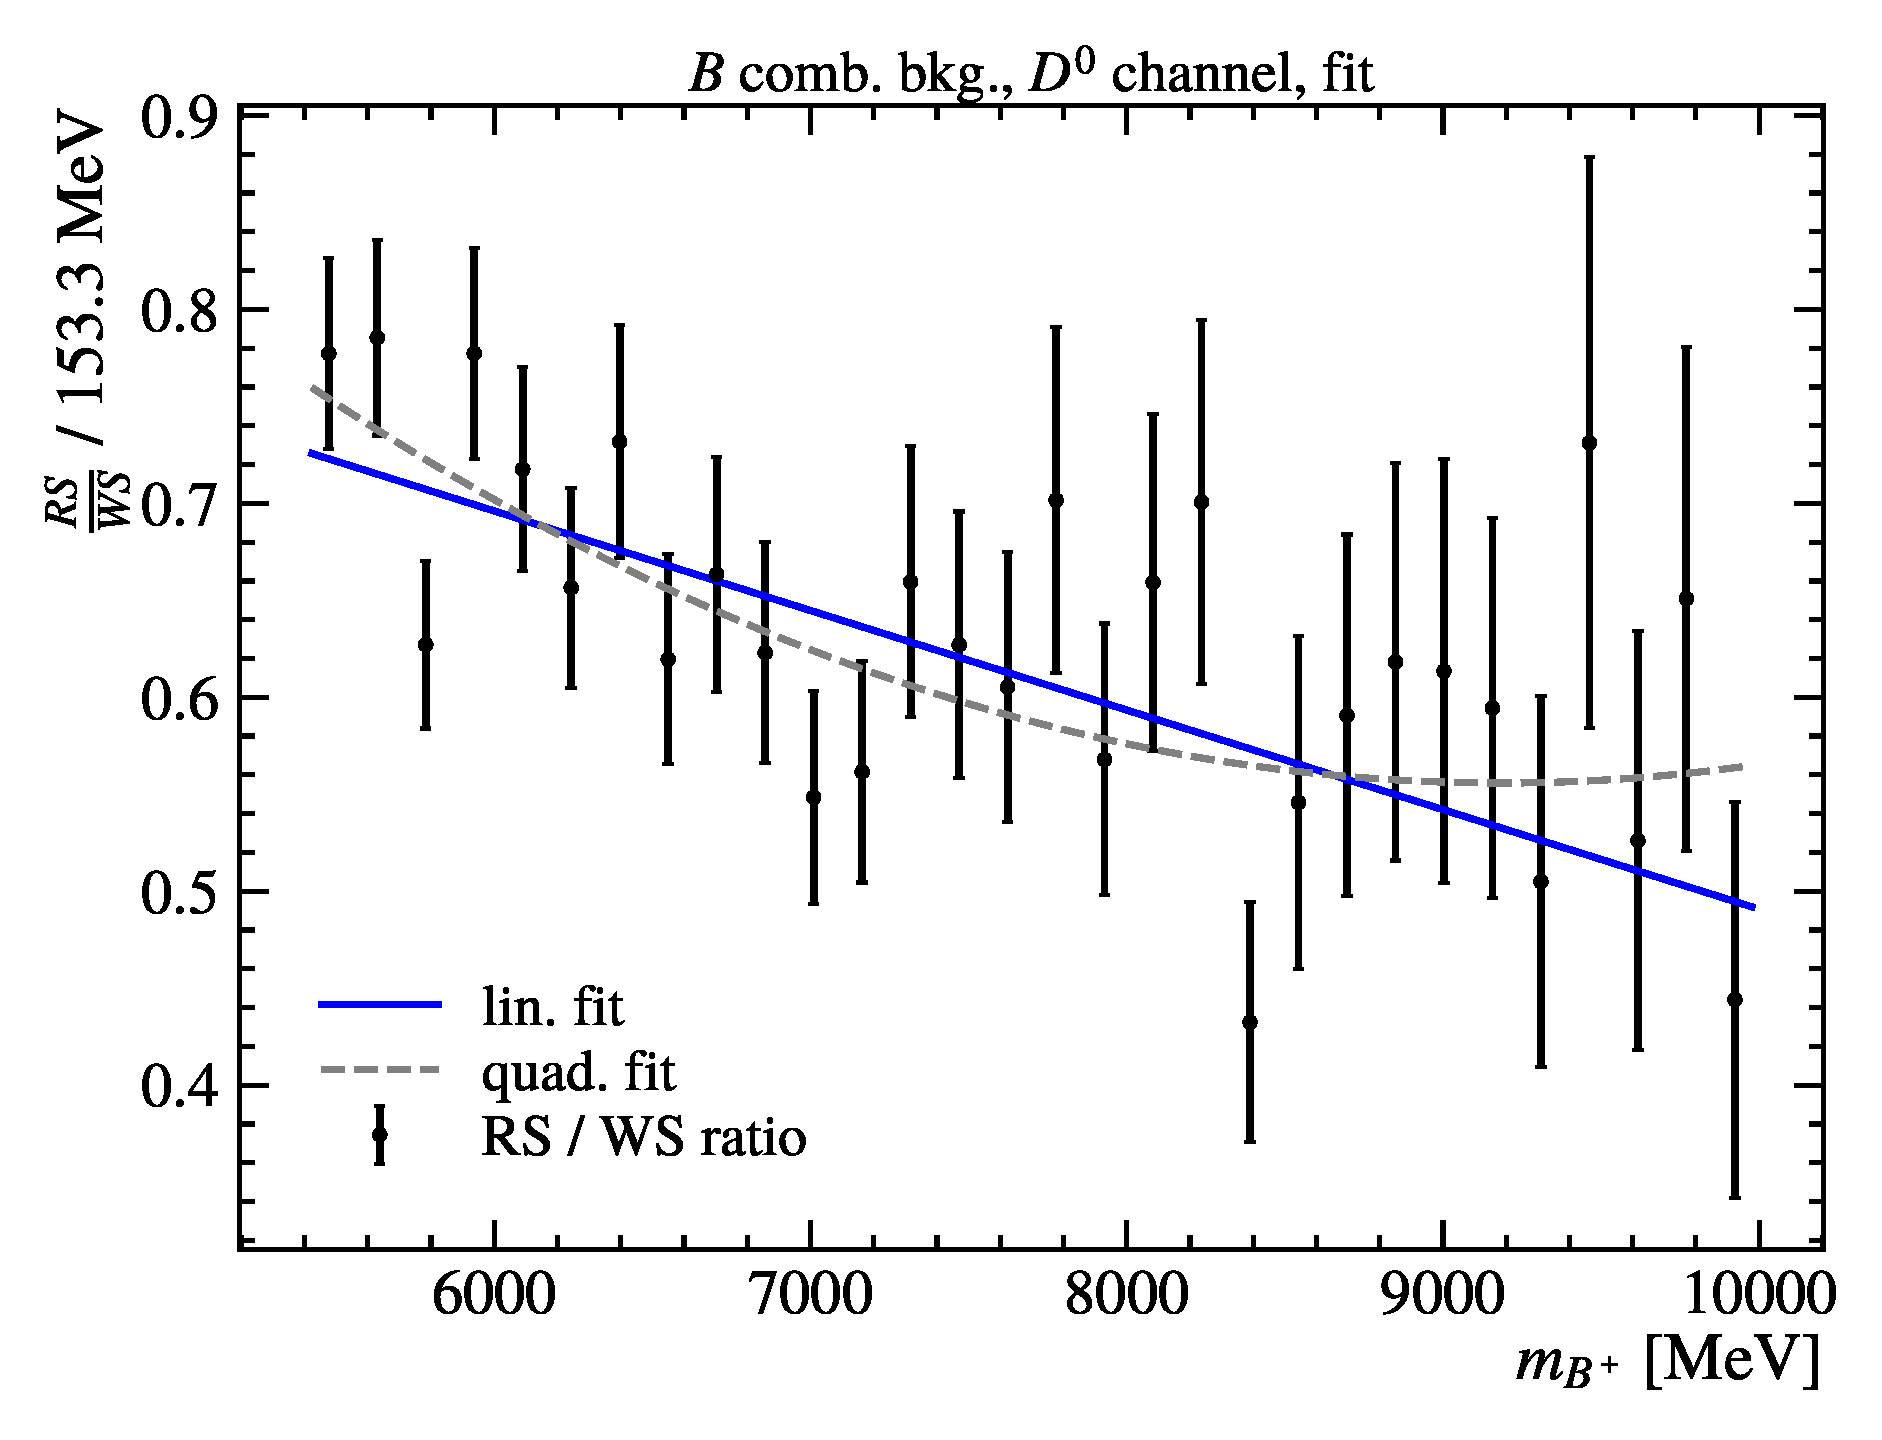
\includegraphics[width=0.48\textwidth]{figs-fit-fit-templates/data-driven-plots/b_comb/fit_b_comb_d0_fit.pdf}
    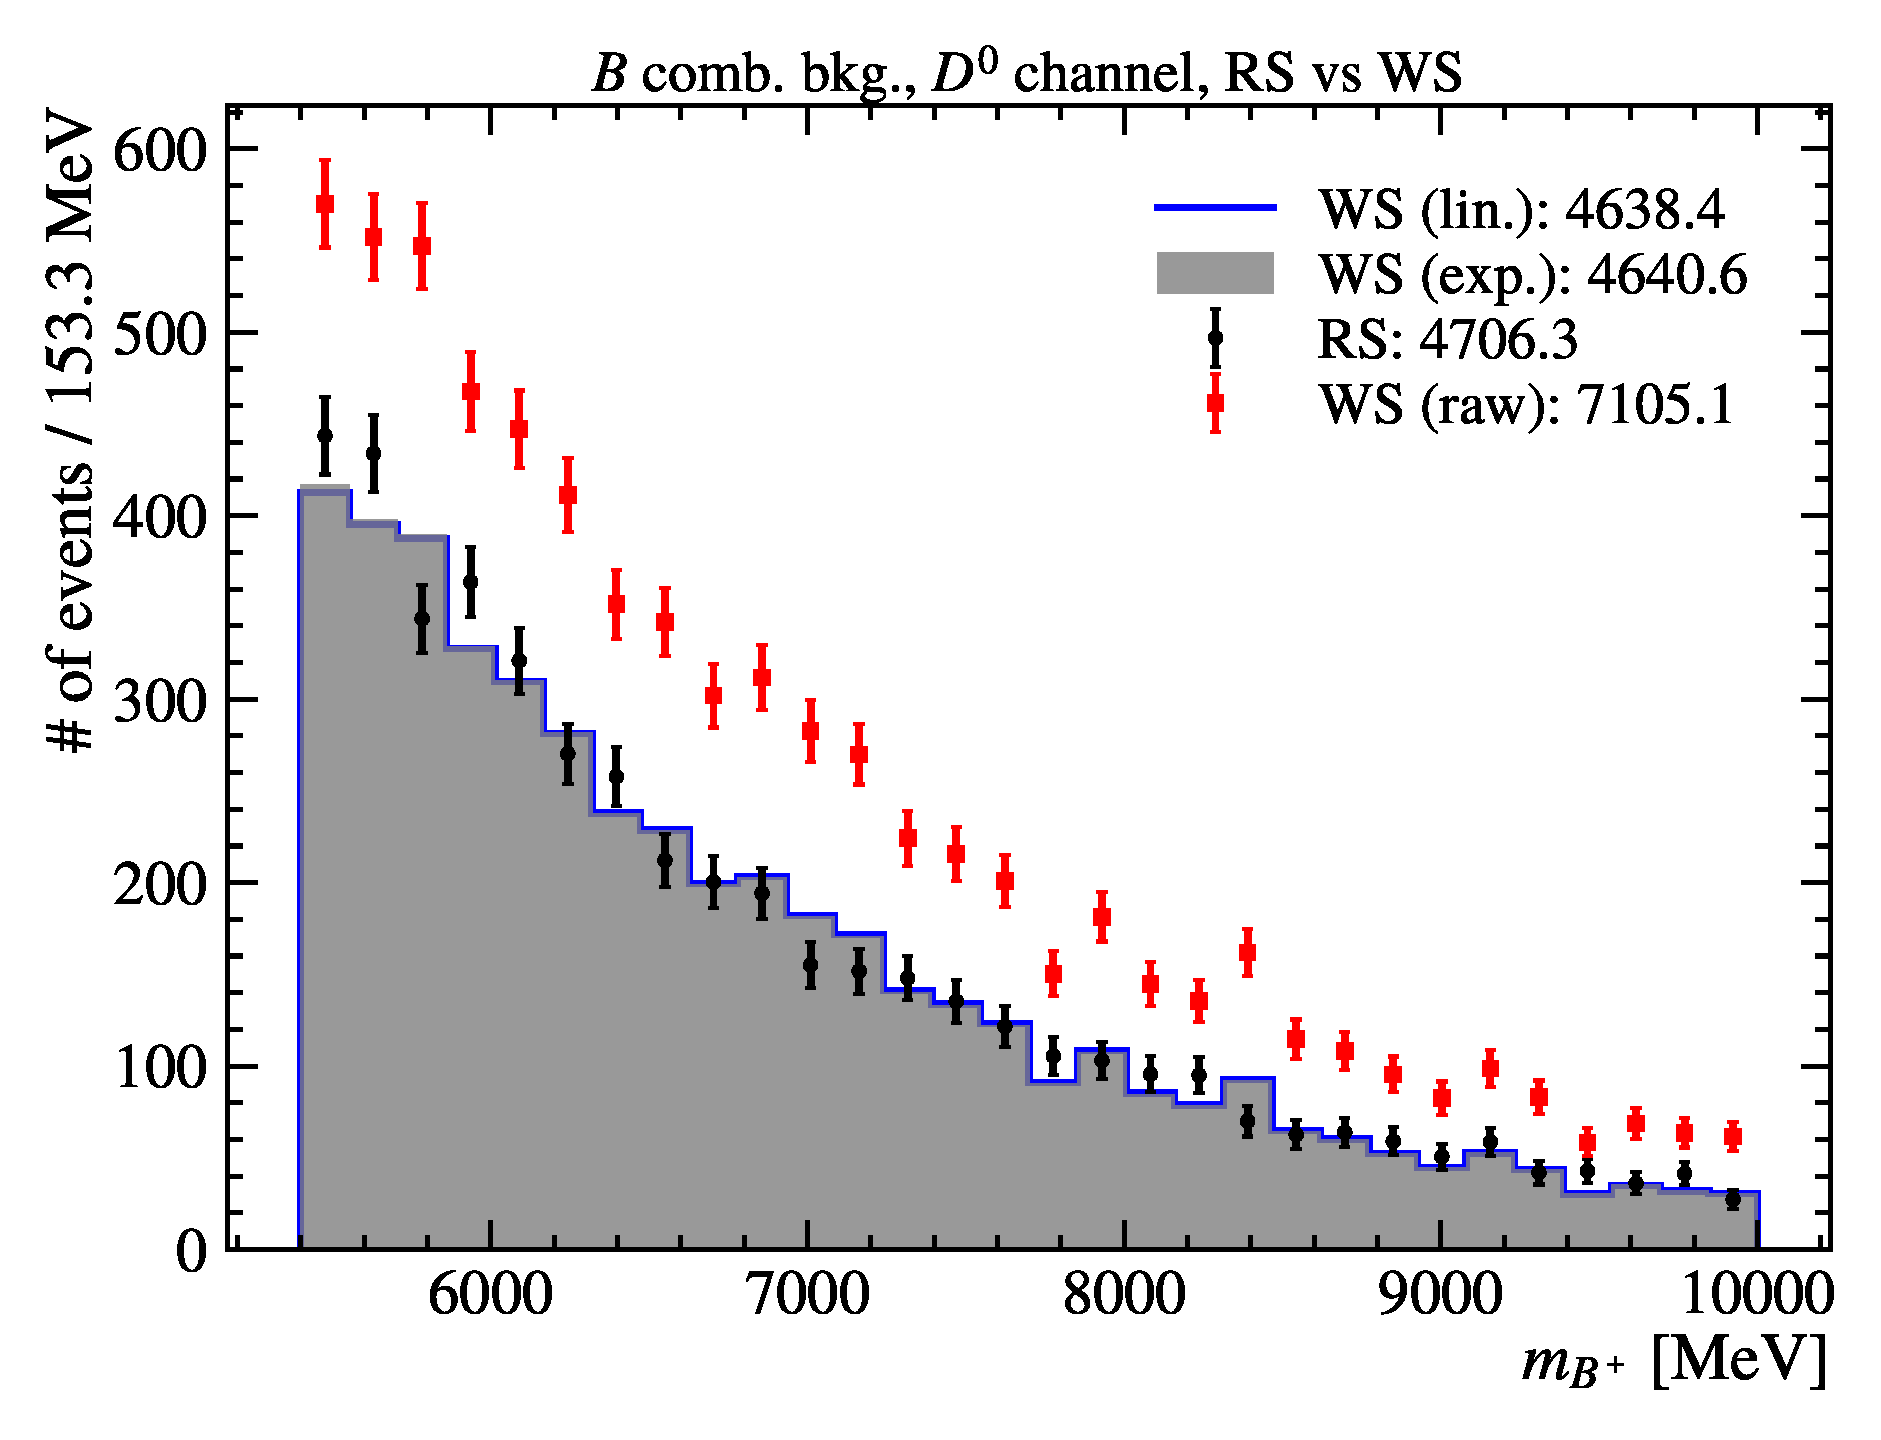
\includegraphics[width=0.48\textwidth]{figs-fit-fit-templates/data-driven-plots/b_comb/fit_b_comb_d0_scaled.pdf}

    \caption{
        \BComb\ fit result for $D^*$ channel.
        Left: \BComb\ auxiliary fit.
        Right: The scaling effect on the WS $\mu$ \BComb\ template.
    }
    \label{fig:b-comb-d0}
\end{figure}


\subsection{Normalization}
\label{tmpl:norm}

\paragraph{$B \rightarrow D^{0,*+}\mun\neumb$}
The yields of these two decay modes,
denoted as \fitNDmu and \fitNmu,
are set to be the free-floating overall normalization for all MC templates of
the respective fit channel.
As a side note,
the \Dz\muon template has notably softer \qSq spectrum compared to
that of \Dstarp\muon due to reduced helicity states available in the
$B \rightarrow D \ell \neulb$ transitions
(discussed in \cref{ref:theory:ff-d0}),
as shown in \cref{fig:d0-norm-vs-dst-norm}.

The \Dstarp\muon mode also contributes to the \Dz channel due to feed down,
with its yield normalized by:
\begin{equation}
    \fitNDmu \times \left\{
        \fitDstISO \times \fitnormfd
    \right\}
\end{equation}
where \fitDstISO is the relative yield ratio between the \Dstarp\muon and
\Dstarz\muon samples:
\begin{equation}
    \fitDstISO =
    \left.\frac{
        \epsilon(\Bzb \rightarrow \Dstarp\mun\neumb)
    }{
        \epsilon(\Bm \rightarrow \Dstarz\mun\neumb)
    }\right|_\text{initial value from MC}^\text{floating in the fit}\times
    \frac{
        \mathcal{B}(\Bzb \rightarrow \Dstarp\mun\neumb)
    }{
        \mathcal{B}(\Bm \rightarrow \Dstarz\mun\neumb)
    }
\end{equation}
where the first ratio, a selection efficiency ratio,
with its initial value obtained with MC samples satisfying the \Dz channel
selection criteria,
is not unity due to different isolation efficiencies for charged
\Dstarp and neutral \Dstarz decays;
the second ratio is the branching fraction ratio attained from external
measurements.
The other parameter \fitnormfd is the yield ratio between the \Dstarz\muon and
\Dz\muon samples:
\begin{equation}
    \fitnormfd =
    \left.\frac{
        \epsilon(\Bm \rightarrow \Dstarz\mun\neumb)
    }{
        \epsilon(\Bm \rightarrow \Dz\mun\neumb)
    }\right|_\text{initially set to 1}^\text{floating in the fit} \times
    \frac{
        \mathcal{B}(\Bm \rightarrow \Dstarz\mun\neumb)
    }{
        \mathcal{B}(\Bm \rightarrow \Dz\mun\neumb)
    }
\end{equation}

%%%%
\paragraph{$B \rightarrow D^{*0}\mun\neumb$}
This mode contributes to the \Dz channel exclusively due to feed down.
Its yield is constrained by
\begin{equation}
    N_{D\mu} \times \fitnormfd
\end{equation}
A comparison between this template and the signal template in the \Dz
channel is also shown in \cref{fig:d0-norm-vs-dst-norm}.

%%%%
\begin{figure}[!htb]
    \begin{subfigure}{\textwidth}
        \centering
        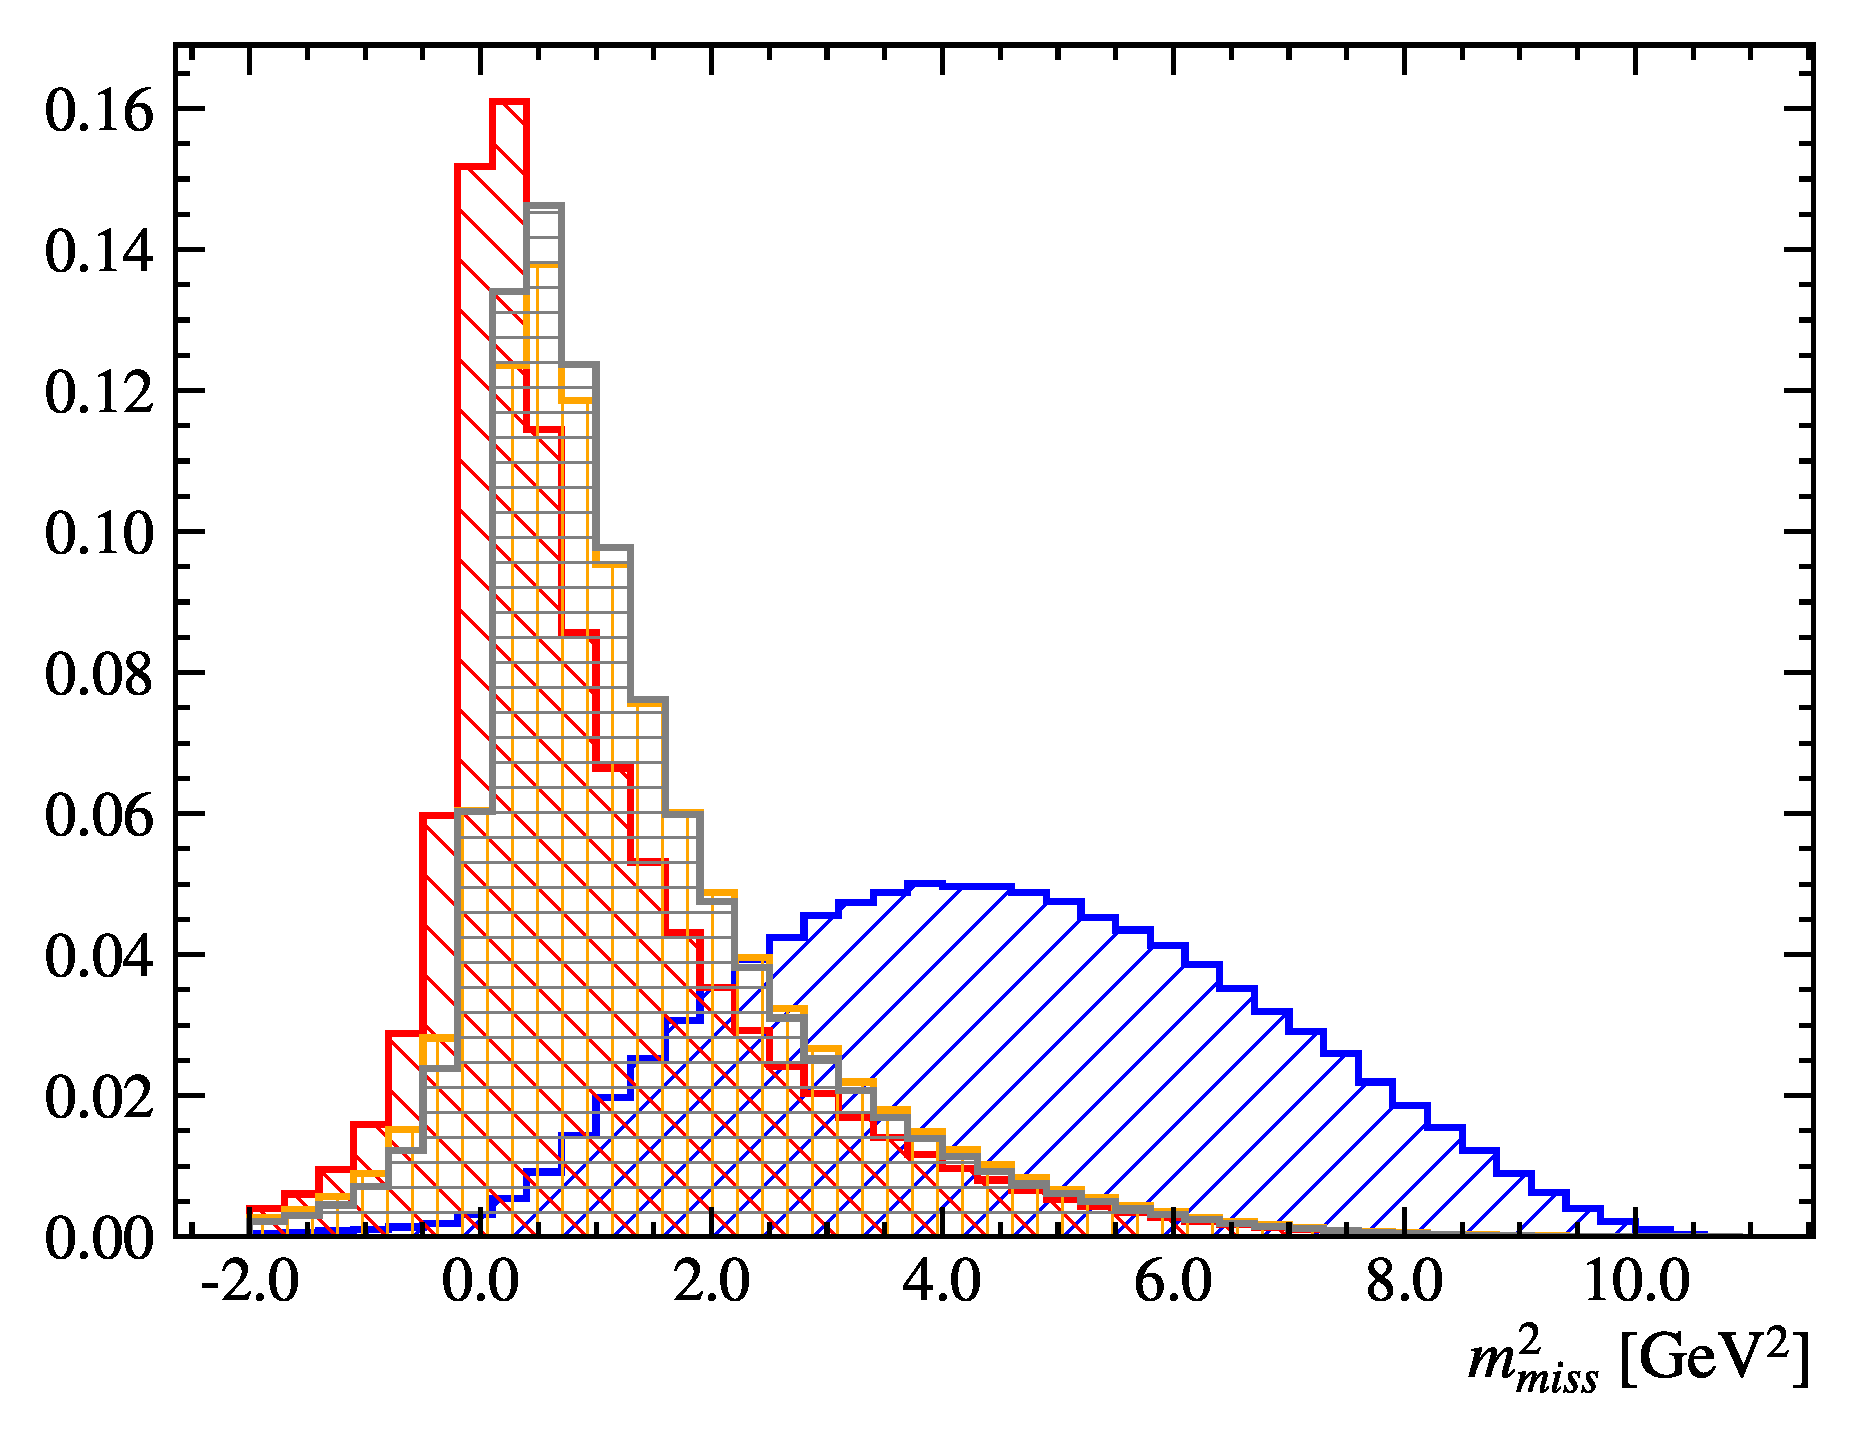
\includegraphics[width=0.3\textwidth]{figs-fit-fit-templates/histo-comp/D0_iso_D0Tau__vs__D0_iso_D0Mu__vs__D0_iso_DstMu__vs__D0_iso_Dst0Mu__m2miss.pdf}
        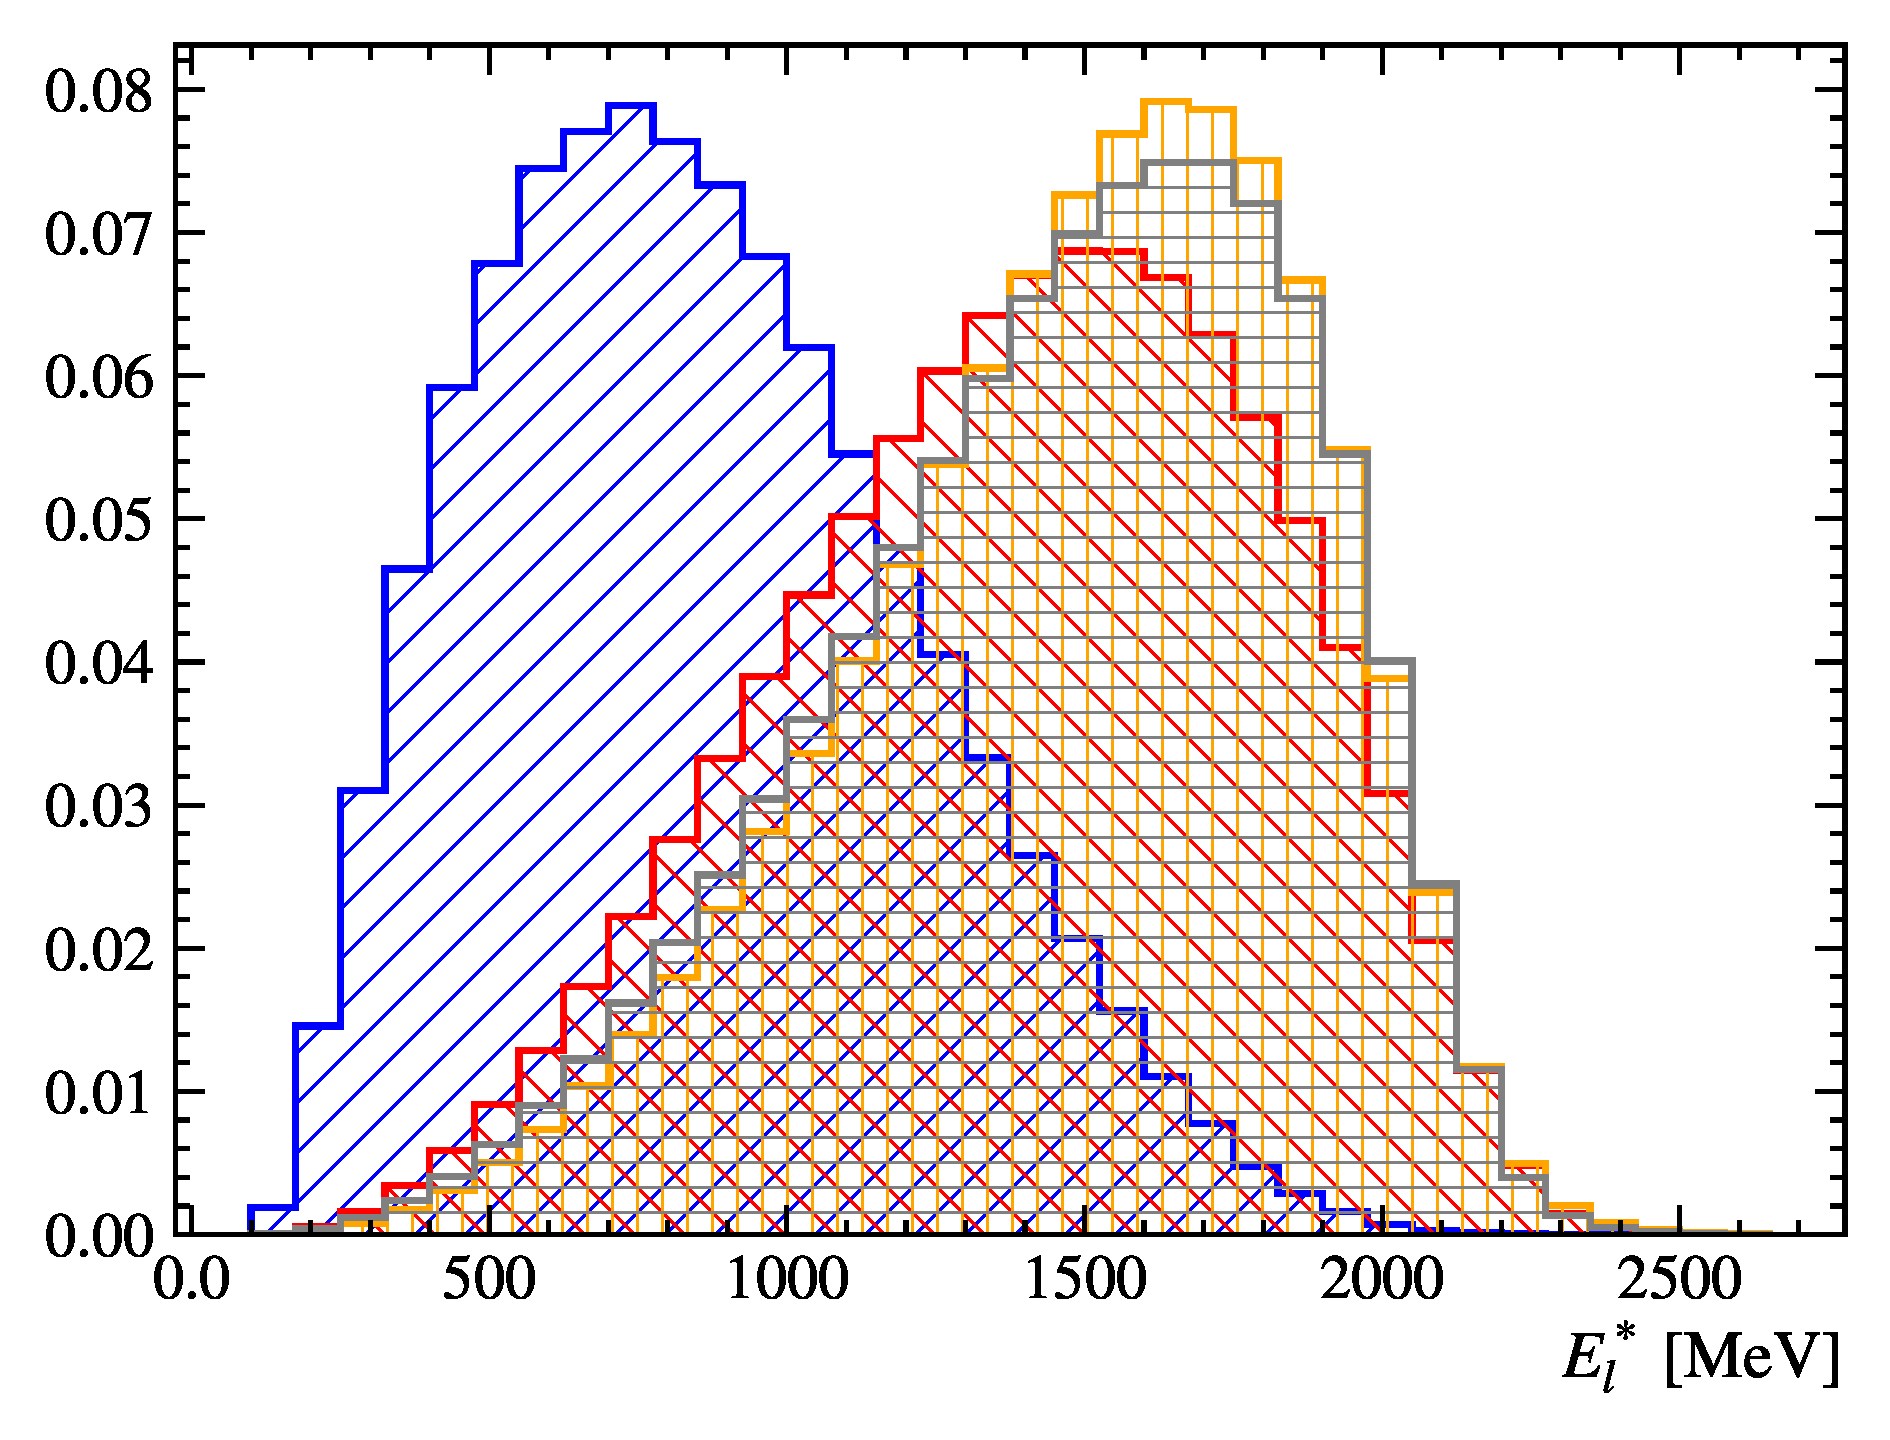
\includegraphics[width=0.3\textwidth]{figs-fit-fit-templates/histo-comp/D0_iso_D0Tau__vs__D0_iso_D0Mu__vs__D0_iso_DstMu__vs__D0_iso_Dst0Mu__el.pdf}
        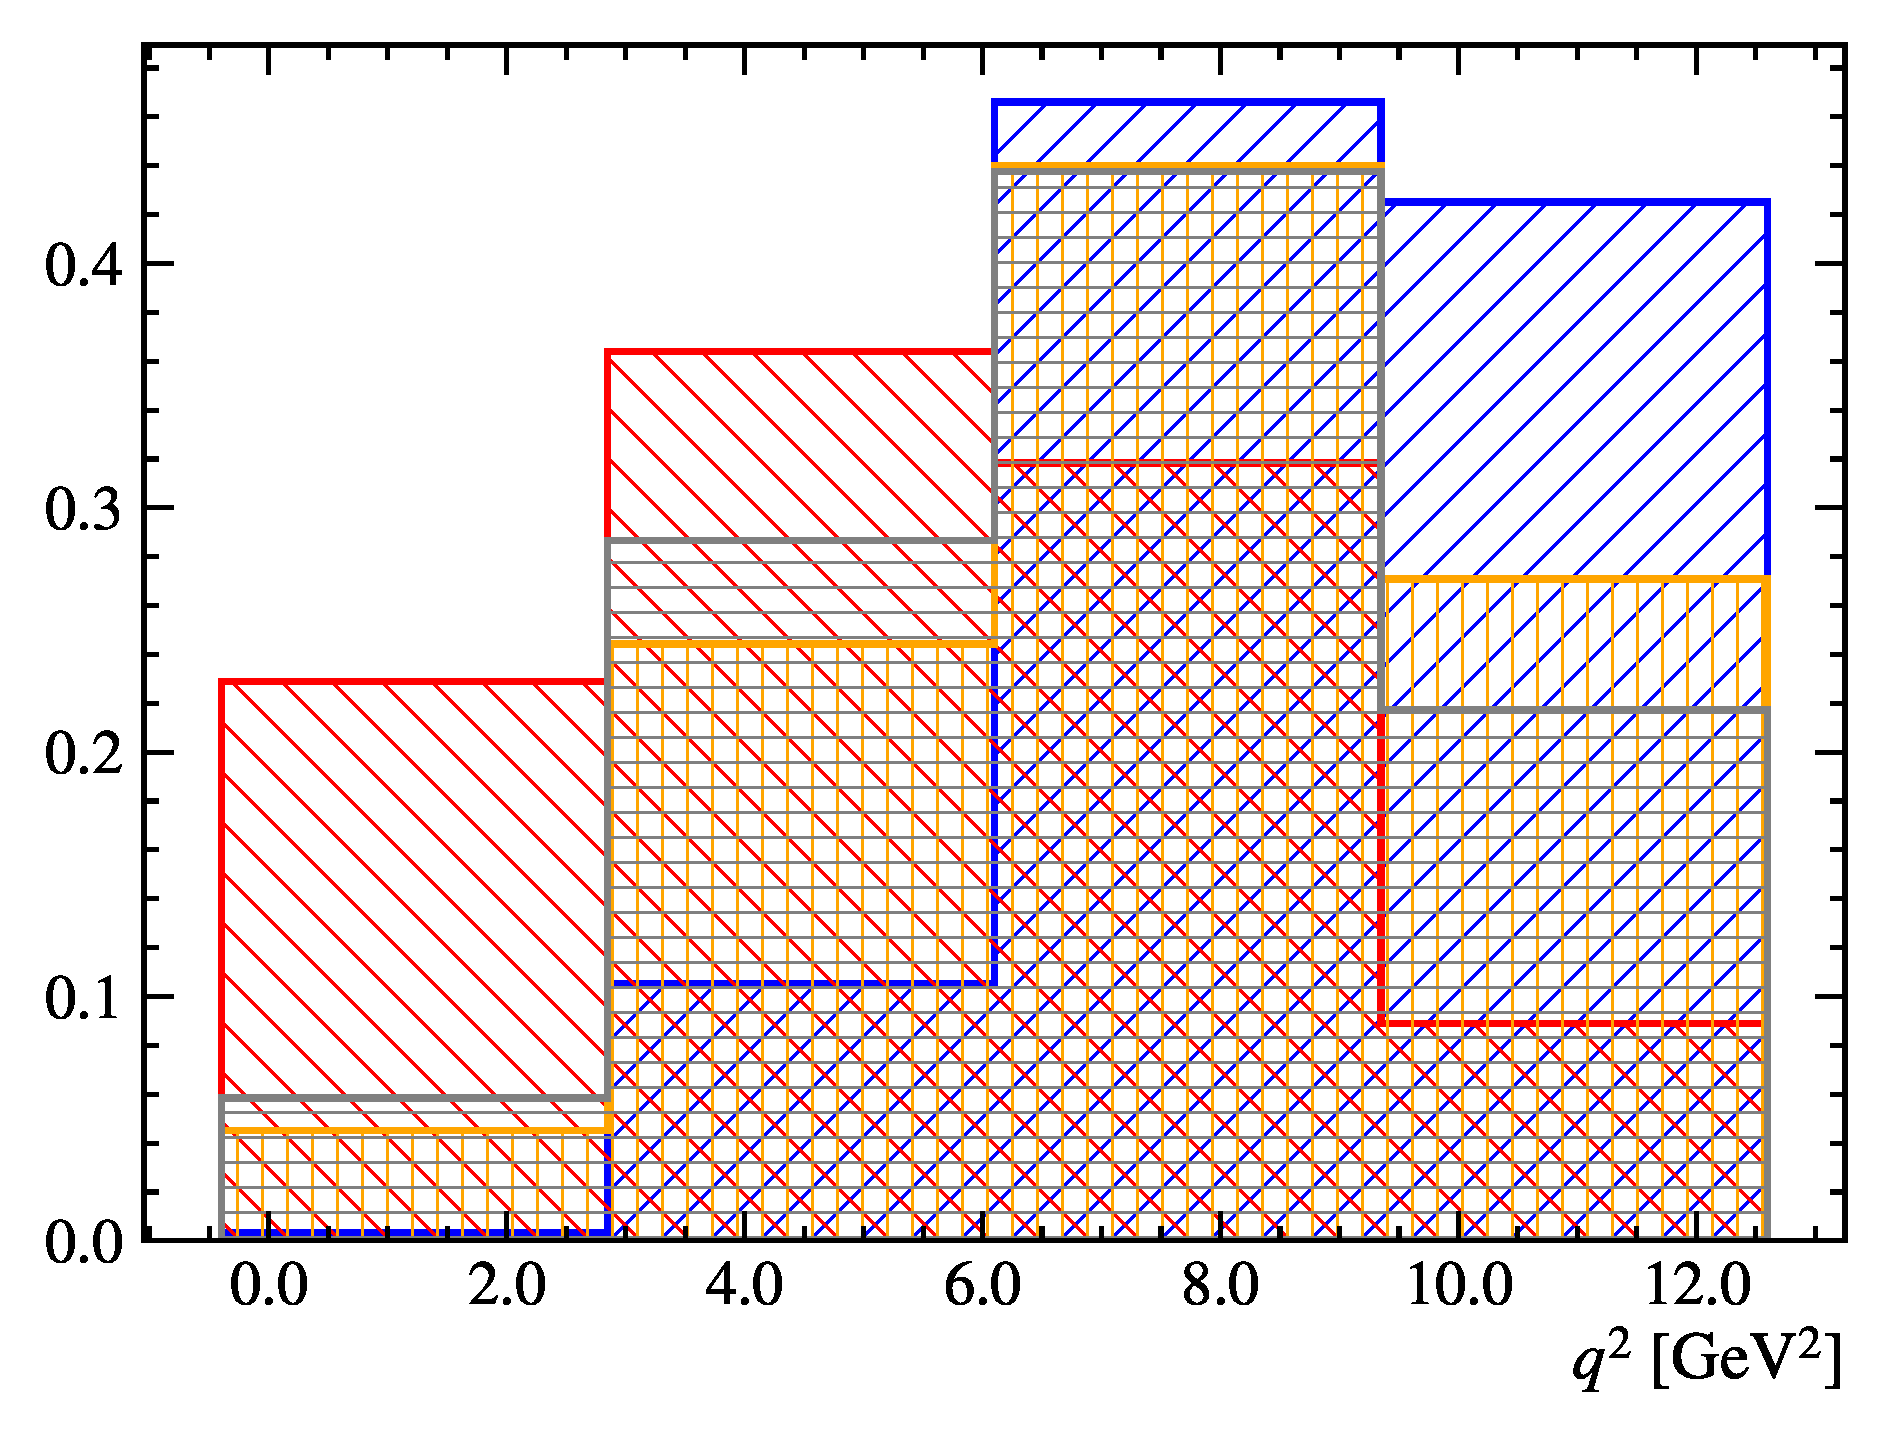
\includegraphics[width=0.3\textwidth]{figs-fit-fit-templates/histo-comp/D0_iso_D0Tau__vs__D0_iso_D0Mu__vs__D0_iso_DstMu__vs__D0_iso_Dst0Mu__q2.pdf}
        \caption{
            $\textcolor{red}{\Bm \rightarrow \Dz\mun\neumb}$
            vs
            $\textcolor{orange}{\Bzb \rightarrow \Dstarp\mun\neumb}$ feed down
            vs
            $\textcolor{gray}{\Bm \rightarrow \Dstarz\mun\neumb}$ feed down.
            All in \Dz channel.
            The signal template
            $\textcolor{blue}{\Bm \rightarrow \Dz\taum\neutb}$
            in the \Dz channel is included as a reference.
        }
    \end{subfigure}

    \begin{subfigure}{\textwidth}
        \centering
        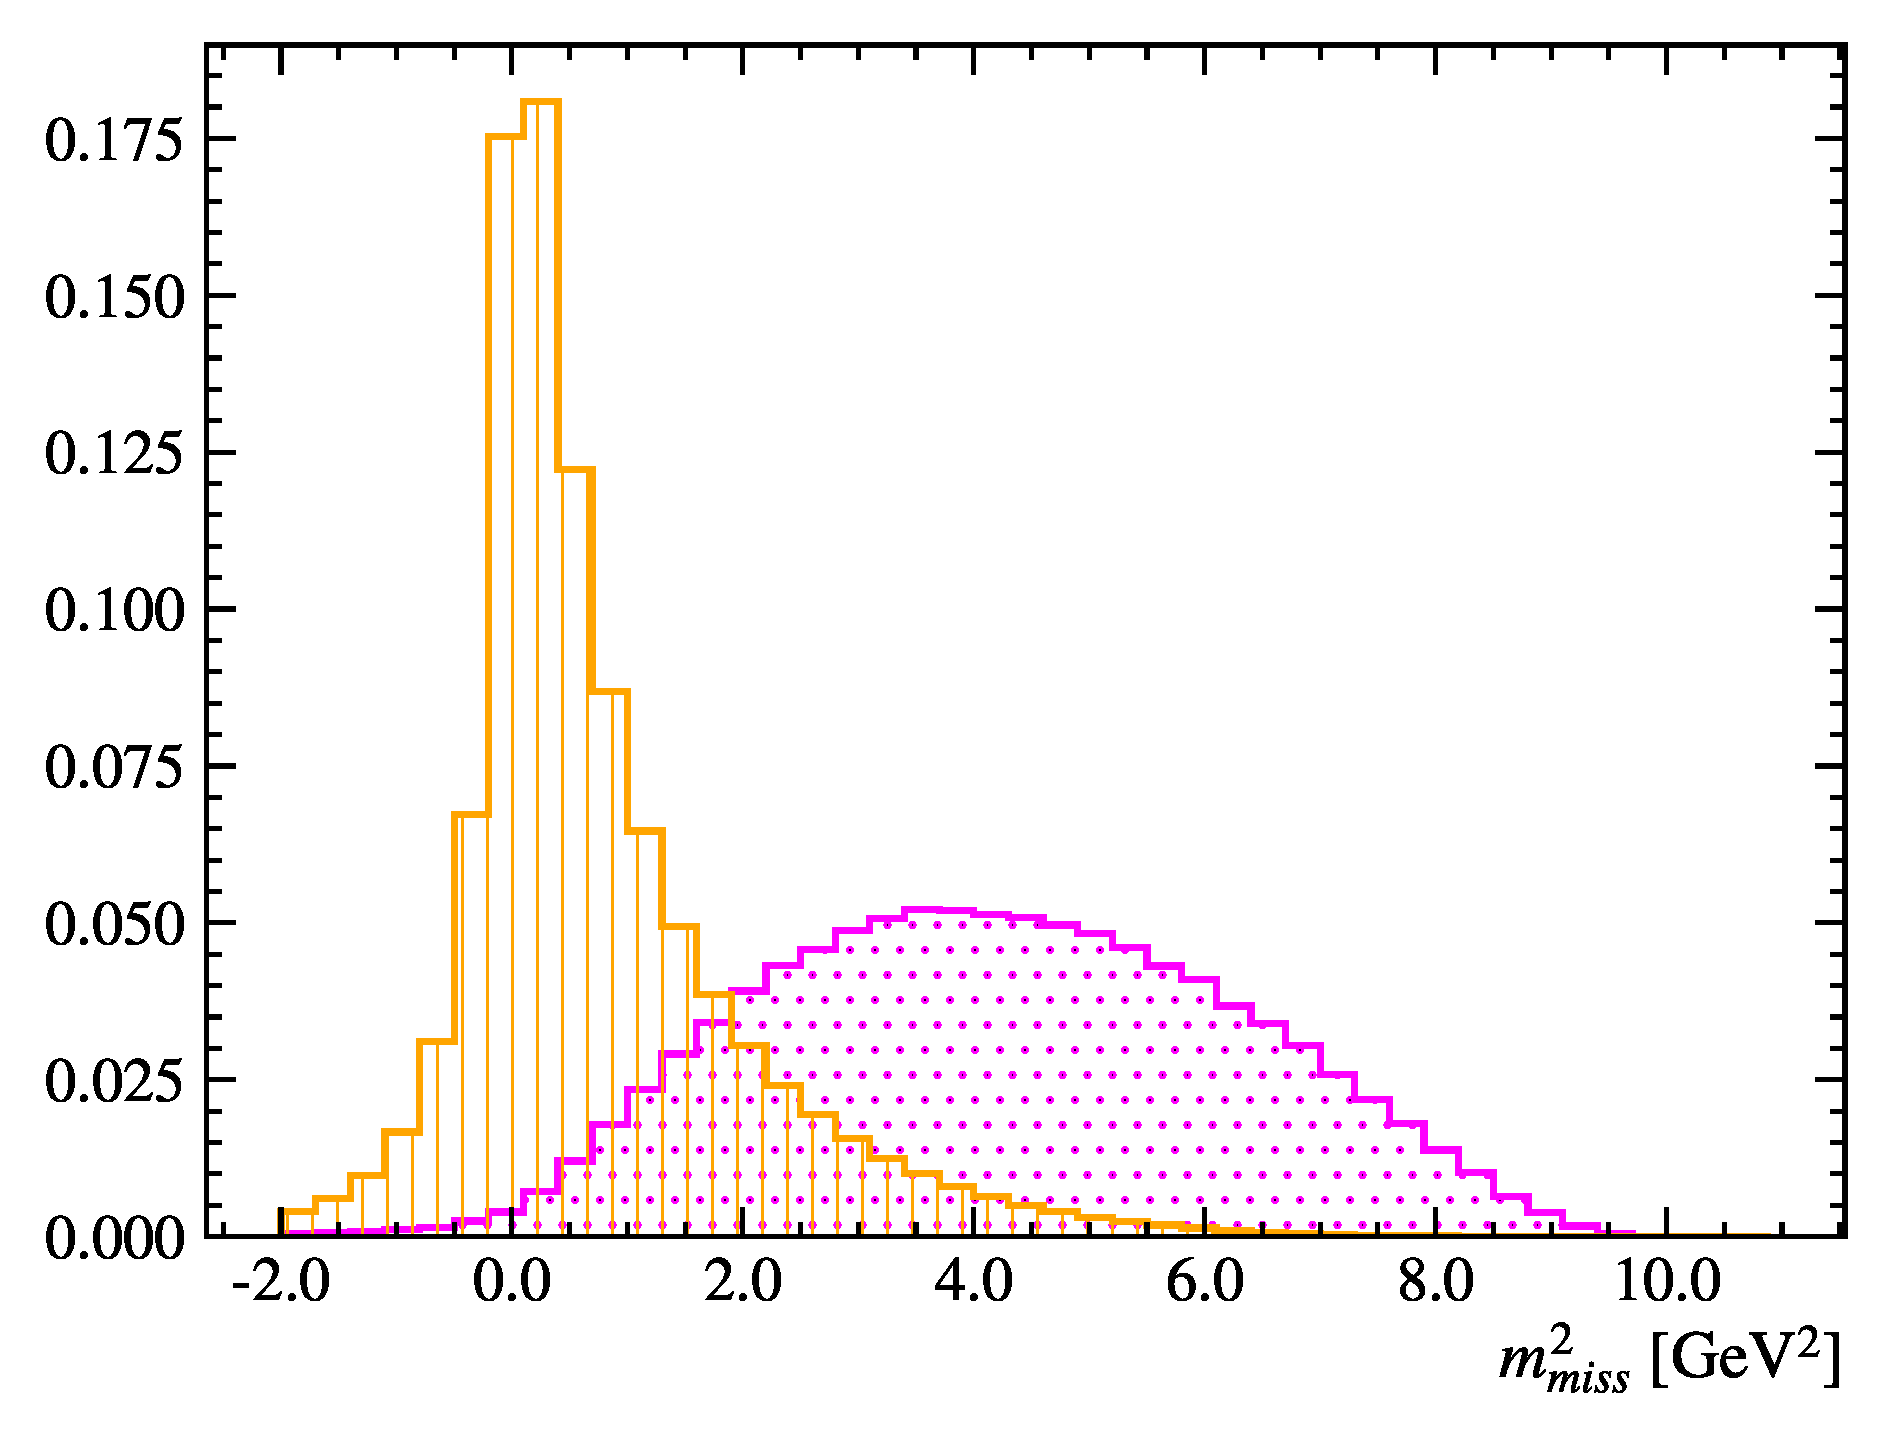
\includegraphics[width=0.3\textwidth]{figs-fit-fit-templates/histo-comp/Dst_iso_DstTau__vs__Dst_iso_DstMu__m2miss.pdf}
        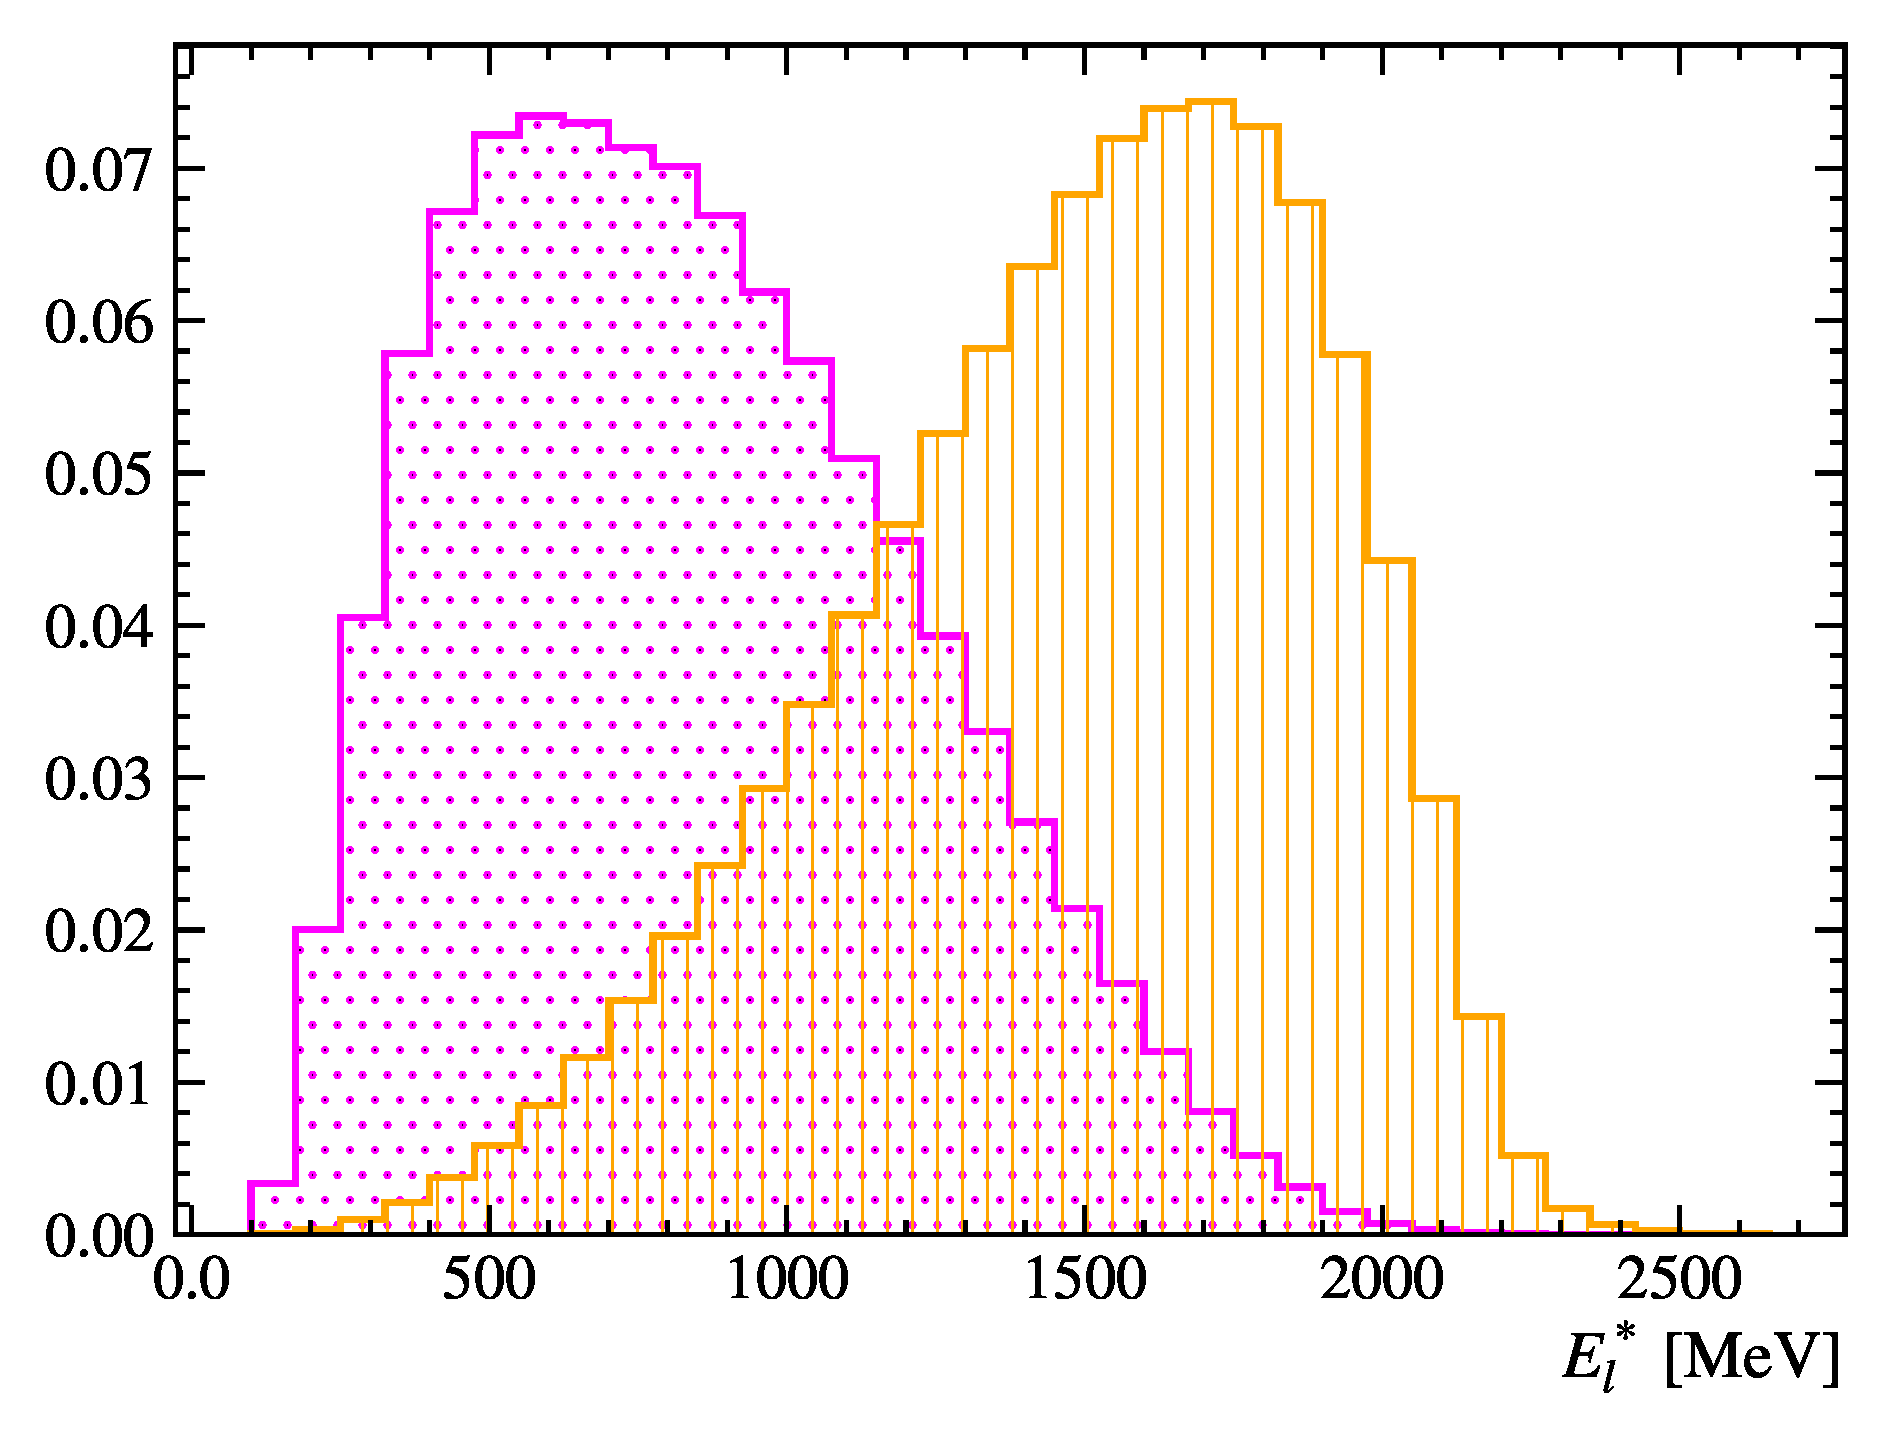
\includegraphics[width=0.3\textwidth]{figs-fit-fit-templates/histo-comp/Dst_iso_DstTau__vs__Dst_iso_DstMu__el.pdf}
        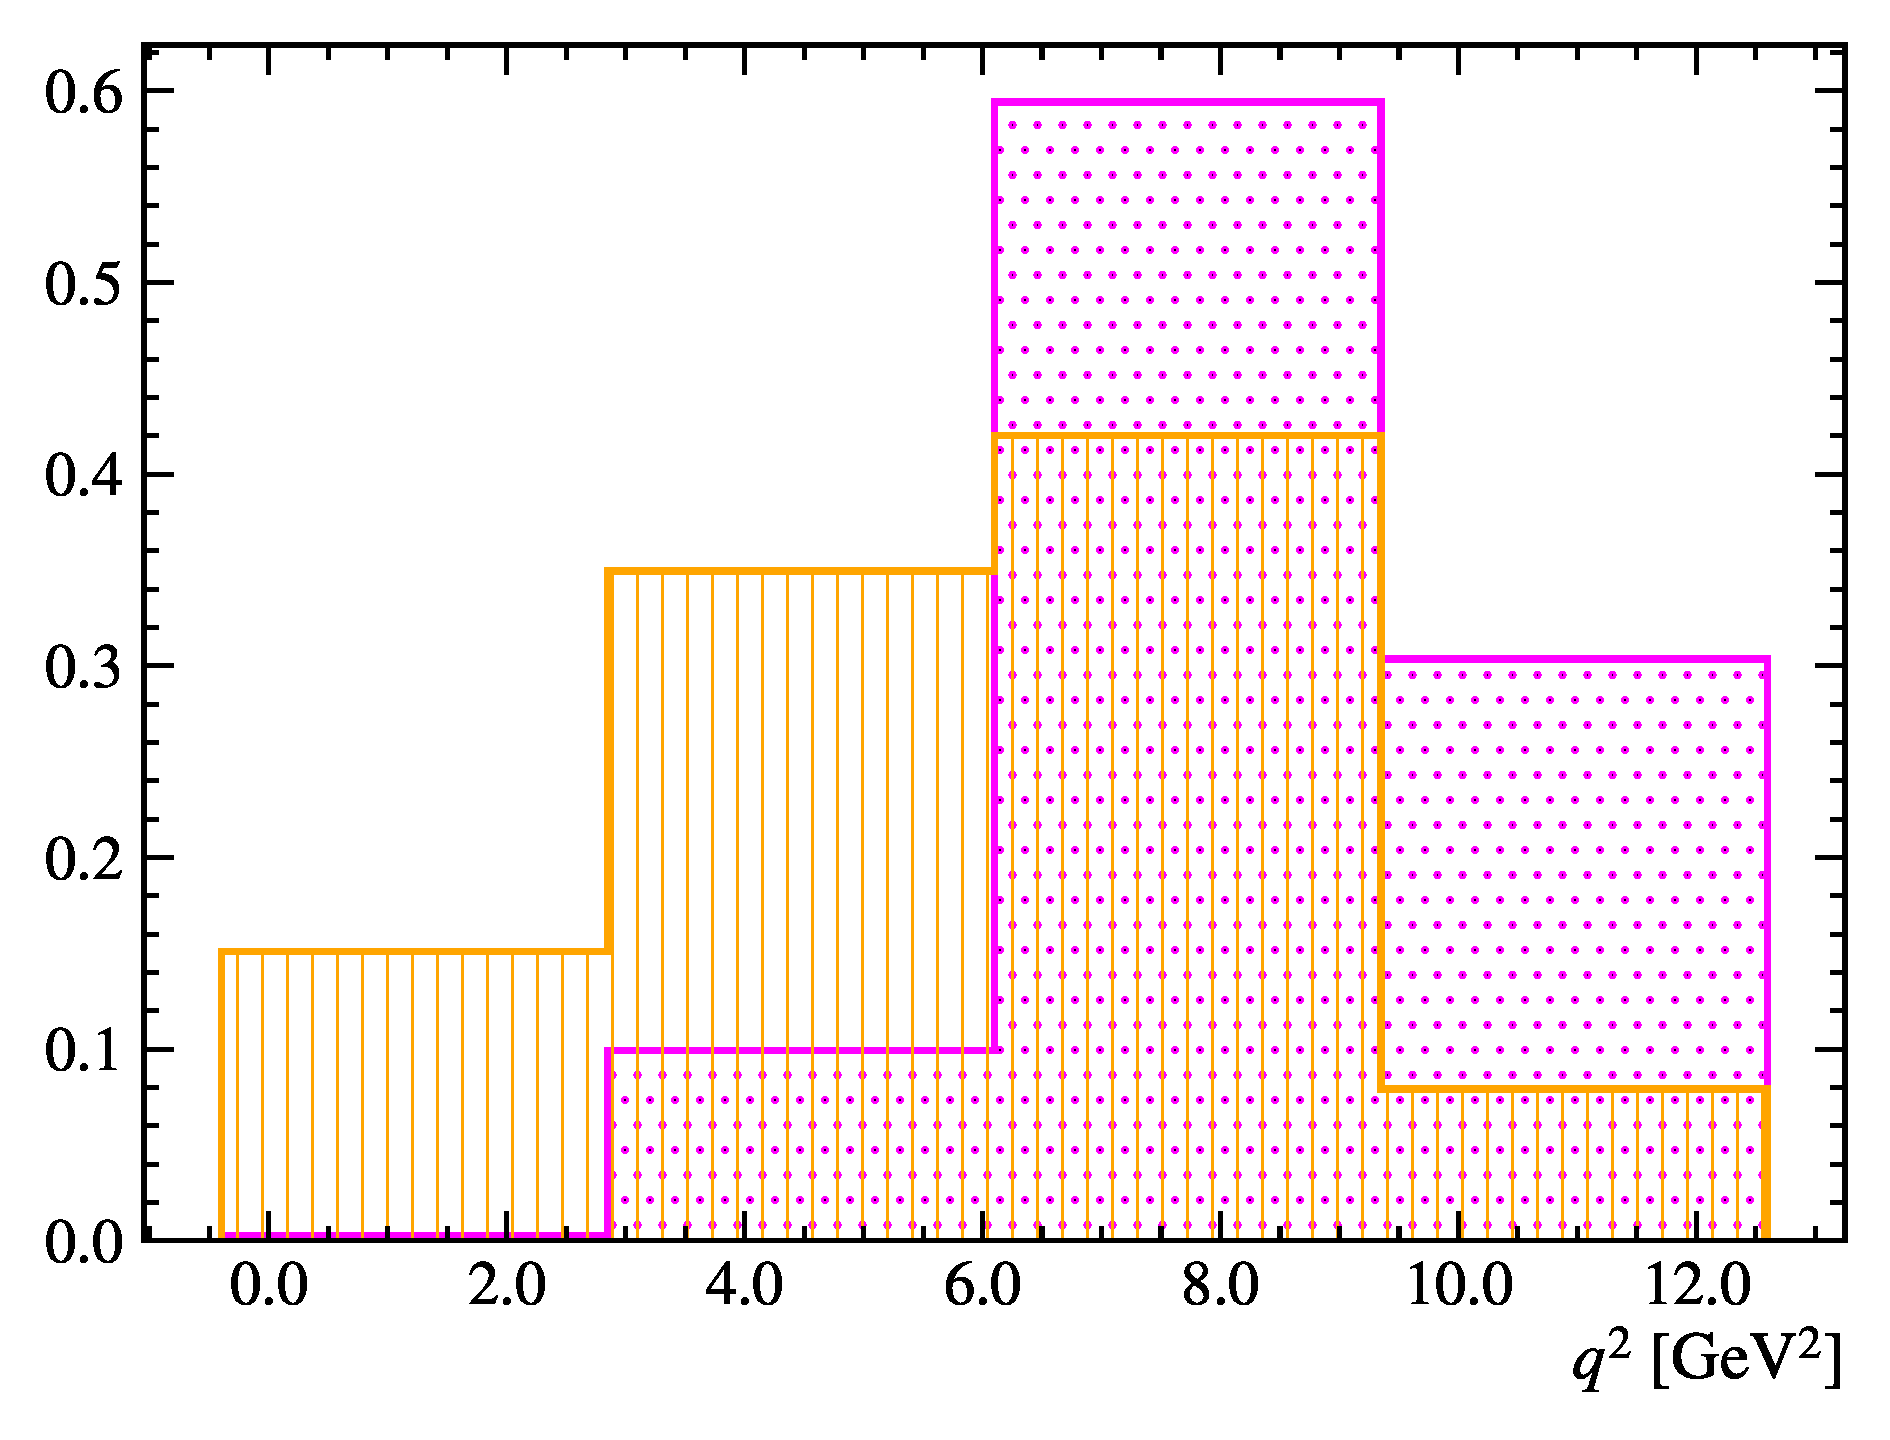
\includegraphics[width=0.3\textwidth]{figs-fit-fit-templates/histo-comp/Dst_iso_DstTau__vs__Dst_iso_DstMu__q2.pdf}
        \caption{
            $\textcolor{orange}{\Bzb \rightarrow \Dstarp\mun\neumb}$ vs
            $\textcolor{magenta}{\Bzb \rightarrow \Dstarp\taum\neutb}$,
            both in \Dstar channel.
        }
    \end{subfigure}

    \caption{
        Comparisons between normalization templates.
    }
    \label{fig:d0-norm-vs-dst-norm}
\end{figure}


\subsection{Signal}
\label{tmpl:sig}

\paragraph{$\Bm \rightarrow \Dz\taum\neutb$}
Its yield is related to $N_{D\mu}$ by the following expression:
\begin{equation}
    N_{D\mu} \times \left\{
        \RD \times \underbrace{
            \BRTauToMu \times
            \frac{
                \epsilon{(\Bm \rightarrow \Dz \taum [\rightarrow \mun\neumb\neut] \neutb)}
            }{
                \epsilon({\Bm \rightarrow \Dz \mun \neumb})
            }
        }_{\equiv \fitRDEff}
    \right\}
\end{equation}
where $\RD \equiv \RDz$ is the free-floating parameter of interest,
and \fitRDEff is the (\tauon leptonic exclusive) efficiency ratio between the
signal and the normalization mode in the \Dz channel,
with the efficiencies obtained with the corresponding MC samples satisfying
the \Dz\muon selection criteria.

%
\paragraph{$B \rightarrow \Dstarp\taum\neutb$}
This signal mode contributes to both channels due to feed down.
In the \Dstar channel, its normalization is given by:
\begin{equation}
    \fitNmu \times \left\{
        \RDst \times \underbrace{
            \BRTauToMu \times \frac{
                \epsilon{(\Bzb \rightarrow \Dstarp \taum [\rightarrow \mun\neumb\neut] \neutb)}_{\Dstar}
            }{
                \epsilon{(\Bzb \rightarrow \Dstarp \mun\neumb)}_{\Dstar}
            }
        }_{\equiv \fitRDstEff}
    \right\}
\end{equation}
where $\RDst \equiv \RDstp$ is the other parameter of interest,
and \fitRDstEff is the efficiency ratio between the signal and the normalization
in the \Dstar channel,
with the tilde emphasizing that the efficiencies are evaluated with the
\Dstarp\muon selection cuts.

Its \Dz channel feed down yield can be formally written as
\begin{align}
    \fitNDmu \times & \Bigg\{
        \overbrace{
            \frac{
                \mathcal{B}(\Bzb \rightarrow \Dstarp \mun\neumb)
            }{
                \mathcal{B}(\Bm \rightarrow \Dz \mun\neumb)
            } \times \frac{
                \epsilon(\Bzb \rightarrow \Dstarp \mun\neumb)
            }{
                \epsilon(\Bm \rightarrow \Dz \mun\neumb)
        }}^{\equiv \fitDstISO \times \fitnormfd} \times
    \nonumber \\
        & \hphantom{\Bigg\{} \underbrace{\BRTauToMu \times \frac{
            \epsilon(\Bzb \rightarrow \Dstarp \taum [\rightarrow \mun\neumb\neut] \neutb)
        }{
            \epsilon(\Bzb \rightarrow \Dstarp \mun\neumb)
        }}_{\equiv \eta_{\Dstarp}\text{, which is not \fitRDstEff!}}
        \times \RDst \Bigg\}
\end{align}
which can then be rewritten as
\begin{equation}
    N_{\Dz\muon} \times \left\{
        \RDst \times \fitRdDstScale \times \fitRDstEff \times \fitDstISO \times \fitnormfd
    \right\}
\end{equation}
noting that $\eta_{\Dstarp}$ is the efficiency ratio evaluated at the \Dz
channel (also notice the lack of a tilde!) and the \BRTauToMu\ cancels in the
second parameter inside the bracket above which is a ratio.


as shown in \cref{fig:d0-sig-vs-d0-norm,fig:dst-sig-vs-dst-norm}.

\begin{figure}[!htb]
    \begin{subfigure}{\textwidth}
        \caption{
            $\Bm \rightarrow \Dz\mun\neumb$ vs.
            $\Bm \rightarrow \Dz\taum\neutb$.
        }
        \label{fig:d0-sig-vs-d0-norm}
    \end{subfigure}

    \begin{subfigure}{\textwidth}
        \caption{
            $\Bzb \rightarrow \Dstarp\mun\neumb$ vs.
            $\Bzb \rightarrow \Dstarp\taum\neutb$.
        }
        \label{fig:dst-sig-vs-dst-norm}
    \end{subfigure}

    \begin{subfigure}{\textwidth}
        \caption{
            $\Bm \rightarrow \Dstarz\mun\neumb$ vs.
            $\Bm \rightarrow \Dstarz\taum\neutb$.
        }
        \label{fig:dst0-sig-vs-dst0-norm}
    \end{subfigure}
    \caption{Comparison between signal and normalization templates.}
\end{figure}

\begin{figure}[!htb]
    \begin{subfigure}{\textwidth}
        \caption{
            $\Bm \rightarrow \Dz\taum\neutb$ vs.
            $\Bzb \rightarrow \Dstarp\taum\neutb$.
        }
        \label{fig:d0-sig-vs-dst-sig}
    \end{subfigure}

    \begin{subfigure}{\textwidth}
        \caption{
            $\Bm \rightarrow \Dz\taum\neutb$ vs.
            $\Bm \rightarrow \Dstarz\taum\neutb$.
        }
        \label{fig:d0-sig-vs-dst0-sig}
    \end{subfigure}

    \caption{Comparison between signal templates.}
\end{figure}

\paragraph{$\Bm \rightarrow D^{*0}\ellm\neulb$}
The \Dstarz ($\rightarrow \Dz \pi$ or $\rightarrow \Dz \gamma$)
in these modes are not reconstructed,
so these templates contribute to the \Dz channel only.
The muonic mode contains an additional branching fraction ratio on top of
$N_{D\mu}$ in its normalization, and is the largest class of contribution
in \Dz data.
For tauonic mode, the \RDstz is set to be equal to \RDstp in the nominal fit.


\subsection{Feed down through $B \rightarrow D^{**}\ellm\neulb$ modes}
\label{tmpl:dstst}

% FIXME: D** descr is pretty bad!
The feed downs from 4 $1P$ $D^{**}$ states
($D_1(2420), D_2^*(2460), D_0^*(2430), D'_1(2430)$, including both isospin
pairs) are included in the fit,
with $10+10$ ($\mu+\tau$) templates in \Dz channel
and $6+6$ in \Dstar.
These $D^{**}$ decay into a \Dz either directly or in a
cascade via a \Dstar or a lighter $D^{**}$,
possibly producing two \emph{charged} \pion
(hence the \Dz\pion\pion templates).

\paragraph{Muonic}
The $D^{**}$ decays often contain unreconstructed \piz or $\gamma$ which leads
to a broad \mmSq distribution peaking at smaller values $\approx m^2_\pion$,
as shown in \cref{fig:dstst-mu-vs-d0-sig}.
The \el spectrum is comparable, but typically softer, than that in normalization,
due to $D^{**}$ states having higher masses compared to \Dz and \Dstar.
These decays are suppressed at zero recoil, as discussed in
\cref{ref:theory:ff-dstst},
but translates weakly in the reconstructed \qSq spectrum, due to rest frame
approximation (\cref{appx:rfa}) and definition of \qSq being
$(p_B - p_D)^2$, instead of $(p_B - p_{D^{**}})^2$.

% FIXME: D** light fit model not understood well.
An overall normalization is shared among all $D^{**}$ modes for \Dstar fit
channel;
Currently, the expected relative yields between each $D^{**}$ are
taken from the run 1 analysis (\cite{LHCb-ANA-2020-056}),
which are computed based on PDG branching fractions.
These branching fractions are multiplied by average isolation efficiencies
for each \B meson type which are found in MC.
Note that the shared normalization factor
$f^\text{nominal}_{D^{**}} \equiv 10^{-3} / \mathcal{B}(B \rightarrow D^{0,*}\mun\neumb)$
is include so that the floating parameters may be read as a branching fractions
times an efficiency directly.

\begin{figure}[!htb]
    %\begin{subfigure}{\textwidth}
    %    \caption{
    %        $\Bm \rightarrow \Dz\taum\neutb$ vs.
    %        $\Bzb \rightarrow \Dstarp\taum\neutb$.
    %    }
    %    \label{fig:d0-sig-vs-dst-sig}
    %\end{subfigure}

    \caption{Comparison between $D^{**}\mu$ and \Dz\taum signal templates.}
    \label{fig:dstst-mu-vs-d0-sig}
\end{figure}

\paragraph{Tauonic}
As in run 1, the tauonic $D^{**}$ decays are treated as fixed fractions
to their muonic counterparts individually, with each $\mathcal{R}(D^{**})$
fraction given by \cite{Bernlochner_2018} within their ``Approximation C'',
for an weighted average of 0.085.
However, the run 1 \RDst analysis (\cite{LHCb-ANA-2014-052}) used
0.12, instead 0.085,
though the values agree within errors specified in that analysis.
Suffice to say, $R(D^{**})$ ratios are not measured to precision.
Therefore, a Gaussian constraint with a width of 30\% is added,
allowing the yields to float around the nominal values.
The Gaussian constraint is shared among all $1P$ $D^{**}$ species within
each fit channel (e.g. \Dz channel) but is distinct across channels.


\subsection{Feed down through $B \rightarrow D_H^{**}(\rightarrow D^{(*)}\pi\pi)\mun\neumb$ modes}

The heavy $D_H^{**}$ decay into either a \Dz or a \Dstar, with two additional
\pion and one of them possibly uncharged.
The fit variables are distributed similar to that in the lighter
$D^{**}$ states.
A comparison between the $D_H^{**}$ templates and \Dz\taum signal can be
seen at \ref{fig:dstst-heavy-vs-d0-sig}

\begin{figure}[!htb]
    %\begin{subfigure}{\textwidth}
    %    \caption{
    %        $\Bm \rightarrow \Dz\taum\neutb$ vs.
    %        $\Bzb \rightarrow \Dstarp\taum\neutb$.
    %    }
    %    \label{fig:d0-sig-vs-dst-sig}
    %\end{subfigure}

    \caption{Comparison between $D_H^{**}\mu$ and \Dz\taum signal templates.}
    \label{fig:dstst-heavy-vs-d0-sig}
\end{figure}


\subsection{Feed down through $\Bsb \rightarrow D_s^{**}\mun\neumb$ modes}

The $D_s^{**}$\footnote{
    More specifically, the $D_{s1}^{'+}$ and $D_{s2}^{*+}$ are included in
    this analysis.
}, daughter of \Bsb, decays into either a $\Kp\Dz$ or $\Kz\Dstarp$.
The former feeds into \Dz channel, whereas the latter feeds into both.
These modes are constrained based on available measurements.
A comparison between the $D_s^{**}$ templates and \Dz\taum signal can be
seen at \cref{fig:d_s-vs-d0-sig}.

\begin{figure}[!htb]
    %\begin{subfigure}{\textwidth}
    %    \caption{
    %        $\Bm \rightarrow \Dz\taum\neutb$ vs.
    %        $\Bzb \rightarrow \Dstarp\taum\neutb$.
    %    }
    %    \label{fig:d0-sig-vs-dst-sig}
    %\end{subfigure}

    \caption{Comparison between $D_s^{**}\mu$ and \Dz\taum signal templates.}
    \label{fig:d_s-vs-d0-sig}
\end{figure}


\subsection{Double-charm ($DDX$) backgrounds}
\label{ref:fit:tmpl:ddx}

The double-charm backgrounds include contributions from
$B \rightarrow D^{(*)}(\rightarrow \mun\neumb)\bar{D}^{(*)} X$ decays, where $X$
is either a \kaon, a \Kstar, or a higher \Kstar resonance.
The $DDX$ are poorly understood as these MC are generated with
a phase space model so generated events are distributed evenly in the available
phase space, without taking the resonance structure,
which itself is not precisely known for $n \geq 3$-body decays,
of the Dalitz plane into account.
Additionally, the $D \rightarrow X \ell\neulb$ decay form factors are
parameterized with the quark-model of ISGW2,
which is known to unable describe data sufficiently well\footnote{
    As commented in \cite{LHCb-ANA-2020-056}:
    ``In the current literature it is found that single-pole-dominance provides
    a much better description of the data than quark-model calculations.''
}.
More details regarding the variations will be discussed in
\cref{ref:fit:var:ddx}.
Both muonic and tauonic $DDX$ templates are similar to the signal templates,
as can be seen in \cref{fig:ddx-vs-d0-sig}.
This is due to the fact that a large portion of energy is taken by the
unreconstructed $D$ meson.

\begin{figure}[!htb]
    %\begin{subfigure}{\textwidth}
    %    \caption{
    %        $\Bm \rightarrow \Dz\taum\neutb$ vs.
    %        $\Bzb \rightarrow \Dstarp\taum\neutb$.
    %    }
    %    \label{fig:d0-sig-vs-dst-sig}
    %\end{subfigure}

    \caption{Comparison between $DDX$ and \Dz\taum signal templates.}
    \label{fig:ddx-vs-d0-sig}
\end{figure}


The relative fractions for the muonic modes are fixed from known branching
fractions at MC generation level.
There is an additional degree of freedom on relative yields between \Bm and \Bzb
with a Gaussian constrain.
Similar to $1P$ $D^{**}$ tauonic modes,
the $DDX$ tauonic modes are constrained near the relative branching fractions
(\tauon vs. \muon) with a 30\% Gaussian variation,
without any degree of freedom on relative yields between \Bm and \Bzb.


% vim: set ft=none:


% Generated in /rdx-run2-analysis, with the command
%   make tab-fit-model-d0
%   make tab-fit-model-dst

\newgeometry{left=0.1in, right=0.1in, top=1in, bottom=1in}
\begin{landscape}
\begin{table}
\centering
\caption{
    Normalization factors for \Dz signal fit with ISO skim templates.
}
\label{tab:fit-norm-fact-d0}
\scriptsize

\begin{tabular}{r|c|c}
\toprule
           \textbf{Alias} &                                 \textbf{Decay mode}                                  &                                                                                                                                                                                  \textbf{Normalization}                                                                                                                                                                                  \\
\midrule
          \texttt{D\_Dmu} &                    $B^- \rightarrow D^0 \mu^- \overline{\nu}_\mu$                    &                                                                                                                                                                                       $N_{D \mu}$                                                                                                                                                                                        \\
       \texttt{D\_dDstmu} &             $\overline{B}^0 \rightarrow D^{*+} \mu^- \overline{\nu}_\mu$             &                                                                                                                                                             $N_{D \mu} \times r_{D^*}^\text{isospin} \times r_{D^{*0}}^{0}$                                                                                                                                                              \\
       \texttt{D\_uDstmu} &                  $B^- \rightarrow D^{*0} \mu^- \overline{\nu}_\mu$                   &                                                                                                                                                                            $N_{D \mu} \times r_{D^{*0}}^{0}$                                                                                                                                                                             \\
         \texttt{D\_Dtau} &                   $B^- \rightarrow D^0 \tau^- \overline{\nu}_\tau$                   &                                                                                                                                                           $N_{D \mu} \times \textcolor{red}{\eta_{D^0}} \times \mathcal{R}(D)$                                                                                                                                                           \\
      \texttt{D\_dDsttau} &            $\overline{B}^0 \rightarrow D^{*+} \tau^- \overline{\nu}_\tau$            &                                                                                        $N_{D \mu} \times \textcolor{red}{\frac{\eta_{D^{*+}}}{\tilde{\eta}_{D^{*+}}}} \times \textcolor{red}{\tilde{\eta}_{D^{*+}}} \times \mathcal{R}(D^*) \times r_{D^{*0}}^{0} \times r_{D^*}^\text{isospin}$                                                                                         \\
      \texttt{D\_uDsttau} &                 $B^- \rightarrow D^{*0} \tau^- \overline{\nu}_\tau$                  &                                                                                                       $N_{D \mu} \times \textcolor{red}{\frac{\eta_{D^{*0}}}{\tilde{\eta}_{D^{*+}}}} \times \textcolor{red}{\tilde{\eta}_{D^{*+}}} \times \mathcal{R}(D^*) \times r_{D^{*0}}^{0}$                                                                                                        \\
        \texttt{D\_dD1mu} &               $\overline{B}^0 \rightarrow D_1 \mu \overline{\nu}_\mu$                &                                                                                      $\textcolor{blue}{\rho^\text{isospin}_{D_1}} \times \textcolor{red}{n^{0}_{D^{**}}} \times N_{D \mu} \times \textcolor{red}{f^{0}_{D_1}} \times \textcolor{red}{\epsilon_{D_1}} \times \mathcal{B}^{0}_{D_1}$                                                                                       \\
  \texttt{D\_dD1mu\_pipi} &   $\overline{B}^0 \rightarrow D_1 (\rightarrow D^0 \pi\pi) \mu \overline{\nu}_\mu$   &                                                                             $\textcolor{blue}{\rho^\text{isospin}_{D_1\pi\pi}} \times \textcolor{red}{n^{0}_{D^{**}}} \times N_{D \mu} \times \textcolor{red}{f^{0}_{D_1}} \times \textcolor{red}{\epsilon_{D_1\pi\pi}} \times \mathcal{B}^{0}_{D_1\pi\pi}$                                                                              \\
        \texttt{D\_dD2mu} &              $\overline{B}^0 \rightarrow D^*_2 \mu \overline{\nu}_\mu$               &                                                                                  $\textcolor{blue}{\rho^\text{isospin}_{D_2^*}} \times \textcolor{red}{n^{0}_{D^{**}}} \times N_{D \mu} \times \textcolor{red}{f^{0}_{D_2^*}} \times \textcolor{red}{\epsilon_{D_2^*}} \times \mathcal{B}^{0}_{D_2^*}$                                                                                   \\
       \texttt{D\_dD1pmu} &               $\overline{B}^0 \rightarrow D'_1 \mu \overline{\nu}_\mu$               &                                                                                    $\textcolor{blue}{\rho^\text{isospin}_{D'_1}} \times \textcolor{red}{n^{0}_{D^{**}}} \times N_{D \mu} \times \textcolor{red}{f^{0}_{D'_1}} \times \textcolor{red}{\epsilon_{D'_1}} \times \mathcal{B}^{0}_{D'_1}$                                                                                     \\
        \texttt{D\_dD0mu} &              $\overline{B}^0 \rightarrow D^*_0 \mu \overline{\nu}_\mu$               &                                                                                  $\textcolor{blue}{\rho^\text{isospin}_{D_1^*}} \times \textcolor{red}{n^{0}_{D^{**}}} \times N_{D \mu} \times \textcolor{red}{f^{0}_{D_1^*}} \times \textcolor{red}{\epsilon_{D_1^*}} \times \mathcal{B}^{0}_{D_1^*}$                                                                                   \\
   \texttt{D\_Dstzpipimu} & $\overline{B} \rightarrow D^{**} (\rightarrow D^{*0} \pi\pi) \mu \overline{\nu}_\mu$ &                                                                                                                                   $\textcolor{red}{n^{0}_{D^{**}}} \times N_{D \mu} \times \textcolor{red}{f_\text{guess}} \times f^0_{D^{*0}\pi\pi}$                                                                                                                                    \\
   \texttt{D\_Dstppipimu} &  $\overline{B} \rightarrow D^{**} (\rightarrow D^* \pi\pi) \mu \overline{\nu}_\mu$   &                                                                                                                                   $\textcolor{red}{n^{0}_{D^{**}}} \times N_{D \mu} \times \textcolor{red}{f_\text{guess}} \times f^0_{D^{*+}\pi\pi}$                                                                                                                                    \\
      \texttt{D\_Dpipimu} &  $\overline{B} \rightarrow D^{**} (\rightarrow D^0 \pi\pi) \mu \overline{\nu}_\mu$   &                                                                                                                                    $\textcolor{red}{n^{0}_{D^{**}}} \times N_{D \mu} \times \textcolor{red}{f_\text{guess}} \times f^0_{D^{0}\pi\pi}$                                                                                                                                    \\
        \texttt{D\_uD1mu} &                    $B^- \rightarrow D_1^0 \mu \overline{\nu}_\mu$                    &                                                                                                         $\textcolor{blue}{\rho^\text{isospin}_{D_1}} \times \textcolor{red}{n^{0}_{D^{**}}} \times N_{D \mu} \times \textcolor{red}{f^{0}_{D_1^0}} \times \mathcal{B}^{0}_{D_1}$                                                                                                         \\
  \texttt{D\_uD1mu\_pipi} &       $B^- \rightarrow D_1^0 (\rightarrow D^0 \pi\pi) \mu \overline{\nu}_\mu$        &                                                                                                   $\textcolor{blue}{\rho^\text{isospin}_{D_1\pi\pi}} \times \textcolor{red}{n^{0}_{D^{**}}} \times N_{D \mu} \times \textcolor{red}{f^{0}_{D_1^0}} \times \mathcal{B}^{0}_{D_1\pi\pi}$                                                                                                   \\
        \texttt{D\_uD2mu} &                  $B^- \rightarrow D_2^{*0} \mu \overline{\nu}_\mu$                   &                                                                                                     $\textcolor{blue}{\rho^\text{isospin}_{D_2^*}} \times \textcolor{red}{n^{0}_{D^{**}}} \times N_{D \mu} \times \textcolor{red}{f^{0}_{D_2^{*0}}} \times \mathcal{B}^{0}_{D_2^*}$                                                                                                      \\
       \texttt{D\_uD1pmu} &                  $B^- \rightarrow {D'_1}^0 \mu \overline{\nu}_\mu$                   &                                                                                                      $\textcolor{blue}{\rho^\text{isospin}_{D'_1}} \times \textcolor{red}{n^{0}_{D^{**}}} \times N_{D \mu} \times \textcolor{red}{f^{0}_{D_1^{'0}}} \times \mathcal{B}^{0}_{D'_1}$                                                                                                       \\
        \texttt{D\_uD0mu} &                  $B^- \rightarrow {D^*_0}^0 \mu \overline{\nu}_\mu$                  &                                                                                                     $\textcolor{blue}{\rho^\text{isospin}_{D_1^*}} \times \textcolor{red}{n^{0}_{D^{**}}} \times N_{D \mu} \times \textcolor{red}{f^{0}_{D_1^{*0}}} \times \mathcal{B}^{0}_{D_1^*}$                                                                                                      \\
       \texttt{D\_sDs2mu} &             $\overline{B}_s \rightarrow D_{s2}^* \mu \overline{\nu}_\mu$             &                                                                                                    $\textcolor{blue}{\mathcal{B}^{*}_{D_{s2}^{*+}}} \times \textcolor{red}{\frac{f_s}{f_d}} \times \textcolor{red}{n^{0}_{D^{**}}} \times \textcolor{red}{N^0_{s2}} \times N_{D \mu}$                                                                                                    \\
      \texttt{D\_sDs1pmu} &             $\overline{B}_s \rightarrow D'_{s1} \mu \overline{\nu}_\mu$              &                                                                                                   $\textcolor{blue}{\mathcal{B}^{*}_{D_{s1}^{'+}}} \times \textcolor{red}{\frac{f_s}{f_d}} \times N_{D \mu} \times \textcolor{red}{n^{0}_{D^{**}}} \times \textcolor{red}{N^0_{s1'}}$                                                                                                    \\
       \texttt{D\_dD1tau} &              $\overline{B}^0 \rightarrow D_1 \tau \overline{\nu}_\tau$               &          $\textcolor{blue}{\rho^\text{isospin}_{D_1}} \times \textcolor{blue}{\rho_{\mathcal{R}(D^{**})}^0} \times \textcolor{red}{n^{0}_{D^{**}}} \times N_{D \mu} \times \textcolor{red}{f^{0}_{D_1}} \times \textcolor{red}{\epsilon_{D_1}} \times \mathcal{B}^{0}_{D_1} \times \textcolor{red}{\mathcal{R}(D^{**})_\text{avg}^\text{raw}} \times \textcolor{red}{r({D_1})}$          \\
 \texttt{D\_dD1tau\_pipi} &  $\overline{B}^0 \rightarrow D_1 (\rightarrow D^0 \pi\pi) \tau \overline{\nu}_\tau$  & $\textcolor{blue}{\rho^\text{isospin}_{D_1\pi\pi}} \times \textcolor{blue}{\rho_{\mathcal{R}(D^{**})}^0} \times \textcolor{red}{n^{0}_{D^{**}}} \times N_{D \mu} \times \textcolor{red}{f^{0}_{D_1}} \times \textcolor{red}{\epsilon_{D_1\pi\pi}} \times \mathcal{B}^{0}_{D_1\pi\pi} \times \textcolor{red}{\mathcal{R}(D^{**})_\text{avg}^\text{raw}} \times \textcolor{red}{r({D_1})}$ \\
       \texttt{D\_dD2tau} &             $\overline{B}^0 \rightarrow D^*_2 \tau \overline{\nu}_\tau$              &     $\textcolor{blue}{\rho^\text{isospin}_{D_2^*}} \times \textcolor{blue}{\rho_{\mathcal{R}(D^{**})}^0} \times \textcolor{red}{n^{0}_{D^{**}}} \times N_{D \mu} \times \textcolor{red}{f^{0}_{D_2^*}} \times \textcolor{red}{\epsilon_{D_2^*}} \times \mathcal{B}^{0}_{D_2^*} \times \textcolor{red}{\mathcal{R}(D^{**})_\text{avg}^\text{raw}} \times \textcolor{red}{r({D_2^*})}$     \\
      \texttt{D\_dD1ptau} &              $\overline{B}^0 \rightarrow D'_1 \tau \overline{\nu}_\tau$              &       $\textcolor{blue}{\rho^\text{isospin}_{D'_1}} \times \textcolor{blue}{\rho_{\mathcal{R}(D^{**})}^0} \times \textcolor{red}{n^{0}_{D^{**}}} \times N_{D \mu} \times \textcolor{red}{f^{0}_{D'_1}} \times \textcolor{red}{\epsilon_{D'_1}} \times \mathcal{B}^{0}_{D'_1} \times \textcolor{red}{\mathcal{R}(D^{**})_\text{avg}^\text{raw}} \times \textcolor{red}{r({D'_1})}$        \\
       \texttt{D\_dD0tau} &             $\overline{B}^0 \rightarrow D^*_0 \tau \overline{\nu}_\tau$              &     $\textcolor{blue}{\rho^\text{isospin}_{D_1^*}} \times \textcolor{blue}{\rho_{\mathcal{R}(D^{**})}^0} \times \textcolor{red}{n^{0}_{D^{**}}} \times N_{D \mu} \times \textcolor{red}{f^{0}_{D_1^*}} \times \textcolor{red}{\epsilon_{D_1^*}} \times \mathcal{B}^{0}_{D_1^*} \times \textcolor{red}{\mathcal{R}(D^{**})_\text{avg}^\text{raw}} \times \textcolor{red}{r({D_1^*})}$     \\
       \texttt{D\_uD1tau} &                   $B^- \rightarrow D_1^0 \tau \overline{\nu}_\tau$                   &                            $\textcolor{blue}{\rho^\text{isospin}_{D_1}} \times \textcolor{blue}{\rho_{\mathcal{R}(D^{**})}^0} \times \textcolor{red}{n^{0}_{D^{**}}} \times N_{D \mu} \times \textcolor{red}{f^{0}_{D_1^0}} \times \mathcal{B}^{0}_{D_1} \times \textcolor{red}{\mathcal{R}(D^{**})_\text{avg}^\text{raw}} \times \textcolor{red}{r({D_1})}$                             \\
 \texttt{D\_uD1tau\_pipi} &       $B^- \rightarrow D_1^0 (\rightarrow D^0 \pi\pi) \mu \overline{\nu}_\tau$       &                      $\textcolor{blue}{\rho^\text{isospin}_{D_1\pi\pi}} \times \textcolor{blue}{\rho_{\mathcal{R}(D^{**})}^0} \times \textcolor{red}{n^{0}_{D^{**}}} \times N_{D \mu} \times \textcolor{red}{f^{0}_{D_1^0}} \times \mathcal{B}^{0}_{D_1\pi\pi} \times \textcolor{red}{\mathcal{R}(D^{**})_\text{avg}^\text{raw}} \times \textcolor{red}{r({D_1})}$                       \\
       \texttt{D\_uD2tau} &                 $B^- \rightarrow D_2^{*0} \tau \overline{\nu}_\tau$                  &                        $\textcolor{blue}{\rho^\text{isospin}_{D_2^*}} \times \textcolor{blue}{\rho_{\mathcal{R}(D^{**})}^0} \times \textcolor{red}{n^{0}_{D^{**}}} \times N_{D \mu} \times \textcolor{red}{f^{0}_{D_2^{*0}}} \times \mathcal{B}^{0}_{D_2^*} \times \textcolor{red}{\mathcal{R}(D^{**})_\text{avg}^\text{raw}} \times \textcolor{red}{r({D_2^*})}$                        \\
      \texttt{D\_uD1ptau} &                 $B^- \rightarrow {D'_1}^0 \tau \overline{\nu}_\tau$                  &                         $\textcolor{blue}{\rho^\text{isospin}_{D'_1}} \times \textcolor{blue}{\rho_{\mathcal{R}(D^{**})}^0} \times \textcolor{red}{n^{0}_{D^{**}}} \times N_{D \mu} \times \textcolor{red}{f^{0}_{D_1^{'0}}} \times \mathcal{B}^{0}_{D'_1} \times \textcolor{red}{\mathcal{R}(D^{**})_\text{avg}^\text{raw}} \times \textcolor{red}{r({D'_1})}$                          \\
       \texttt{D\_uD0tau} &                 $B^- \rightarrow {D^*_0}^0 \tau \overline{\nu}_\tau$                 &                        $\textcolor{blue}{\rho^\text{isospin}_{D_1^*}} \times \textcolor{blue}{\rho_{\mathcal{R}(D^{**})}^0} \times \textcolor{red}{n^{0}_{D^{**}}} \times N_{D \mu} \times \textcolor{red}{f^{0}_{D_1^{*0}}} \times \mathcal{B}^{0}_{D_1^*} \times \textcolor{red}{\mathcal{R}(D^{**})_\text{avg}^\text{raw}} \times \textcolor{red}{r({D_1^*})}$                        \\
        \texttt{D\_dDDmu} &    $\overline{B}^0 \rightarrow D^0 D_q (\rightarrow \mu \overline{\nu}_\mu X') X$    &                                                                                                                                      $\textcolor{magenta}{\rho^0_{DDX,u/d}} \times f^0_{DDX} \times N_{D \mu} \times \textcolor{red}{f^0_{DDX,d}}$                                                                                                                                       \\
        \texttt{D\_uDDmu} &         $B^- \rightarrow D^0 D_q (\rightarrow \mu \overline{\nu}_\mu X') X$          &                                                                                                                                      $\textcolor{magenta}{\rho^0_{DDX,u/d}} \times f^0_{DDX} \times N_{D \mu} \times \textcolor{red}{f^0_{DDX,u}}$                                                                                                                                       \\
       \texttt{D\_dDDtau} &   $\overline{B}^0 \rightarrow D^0 D_q (\rightarrow \tau \overline{\nu}_\tau X') X$   &                                                                                     $\textcolor{blue}{\rho^0_\text{isolation,\tau}} \times \textcolor{magenta}{\rho^0_{DDX,u/d}} \times \textcolor{red}{f^0_{DDX,\tau}} \times f^0_{DDX} \times N_{D \mu} \times \textcolor{red}{f^0_{DDX,d,\tau}}$                                                                                      \\
       \texttt{D\_uDDtau} &        $B^- \rightarrow D^0 D_q (\rightarrow \tau \overline{\nu}_\tau X') X$         &                                                                                     $\textcolor{blue}{\rho^0_\text{isolation,\tau}} \times \textcolor{magenta}{\rho^0_{DDX,u/d}} \times \textcolor{red}{f^0_{DDX,\tau}} \times f^0_{DDX} \times N_{D \mu} \times \textcolor{red}{f^0_{DDX,u,\tau}}$                                                                                      \\
         \texttt{D\_comb} &                                   $B^-$ comb. bkg.                                   &                                                                                                                                                  $\textcolor{blue}{\rho^0_\text{$B$ comb}} \times \textcolor{red}{N^0_\text{$B$ comb}}$                                                                                                                                                  \\
        \texttt{D\_misID} &                                        misID.                                        &                                                                                                                                                     $\textcolor{blue}{\rho^0_\text{misID}} \times \textcolor{red}{N^0_\text{misID}}$                                                                                                                                                     \\
\bottomrule
\end{tabular}

\end{table}
\end{landscape}
\restoregeometry


\begin{landscape}
\begin{table}
\centering
\caption{
    Normalization factors for \Dstar signal fit with ISO skim templates.
}
\label{tab:fit-norm-fact-dst}
\scriptsize

\begin{tabular}{r|c|c}
\toprule
        \textbf{Alias} &                                \textbf{Decay mode}                                &                                                                                                                                                                                             \textbf{Normalization}                                                                                                                                                                                              \\
\midrule
   \texttt{Dst\_sigmu} &           $\overline{B}^0 \rightarrow D^{*+} \mu^- \overline{\nu}_\mu$            &                                                                                                                                                                                                  $N_{D^* \mu}$                                                                                                                                                                                                  \\
  \texttt{Dst\_sigtau} &          $\overline{B}^0 \rightarrow D^{*+} \tau^- \overline{\nu}_\tau$           &                                                                                                                                                               $N_{D^* \mu} \times \mathcal{R}(D^*) \times \textcolor{red}{\tilde{\eta}_{D^{*+}}}$                                                                                                                                                               \\
      \texttt{Dst\_D1} &              $\overline{B}^0 \rightarrow D_1 \mu \overline{\nu}_\mu$              &                                                                                           $\textcolor{blue}{\mathcal{B}^{*}_{D_1}} \times \textcolor{blue}{\mathcal{B}^*_{D^{**}}} \times \textcolor{red}{n^{*}_{D^{**}}} \times N_{D^* \mu} \times \textcolor{red}{f^{*}_{D_1}} \times \textcolor{red}{\frac{1}{2}}$                                                                                           \\
      \texttt{Dst\_D2} &             $\overline{B}^0 \rightarrow D^*_2 \mu \overline{\nu}_\mu$             &                                                                                         $\textcolor{blue}{\mathcal{B}^{*}_{D_2^*}} \times \textcolor{blue}{\mathcal{B}^*_{D^{**}}} \times \textcolor{red}{n^{*}_{D^{**}}} \times N_{D^* \mu} \times \textcolor{red}{f^{*}_{D_2^*}} \times \textcolor{red}{\frac{1}{2}}$                                                                                         \\
     \texttt{Dst\_D1p} &             $\overline{B}^0 \rightarrow D'_1 \mu \overline{\nu}_\mu$              &                                                                                          $\textcolor{blue}{\mathcal{B}^{*}_{D'_1}} \times \textcolor{blue}{\mathcal{B}^*_{D^{**}}} \times \textcolor{red}{n^{*}_{D^{**}}} \times N_{D^* \mu} \times \textcolor{red}{f^{*}_{D'_1}} \times \textcolor{red}{\frac{1}{2}}$                                                                                          \\
   \texttt{Dst\_D2Smu} & $\overline{B} \rightarrow D^{**} (\rightarrow D^* \pi\pi) \mu \overline{\nu}_\mu$ &                                                                                                                                                                 $\textcolor{red}{n^{*}_{D^{**}}} \times N_{D^* \mu} \times f^*_{D^{*+}\pi\pi}$                                                                                                                                                                  \\
     \texttt{Dst\_uD1} &                  $B^- \rightarrow D_1^0 \mu \overline{\nu}_\mu$                   &                                                                                 $\textcolor{blue}{\mathcal{B}^{*}_{D_1^0}} \times \textcolor{blue}{\mathcal{B}^*_{D^{**}}} \times \textcolor{blue}{\epsilon_\text{isolation}} \times \textcolor{red}{n^{*}_{D^{**}}} \times N_{D^* \mu} \times \textcolor{red}{f^{*}_{D_1^0}}$                                                                                  \\
     \texttt{Dst\_uD2} &                 $B^- \rightarrow D_2^{*0} \mu \overline{\nu}_\mu$                 &                                                                              $\textcolor{blue}{\mathcal{B}^{*}_{D_2^{*0}}} \times \textcolor{blue}{\mathcal{B}^*_{D^{**}}} \times \textcolor{blue}{\epsilon_\text{isolation}} \times \textcolor{red}{n^{*}_{D^{**}}} \times N_{D^* \mu} \times \textcolor{red}{f^{*}_{D_2^{*0}}}$                                                                               \\
    \texttt{Dst\_uD1p} &                 $B^- \rightarrow {D'_1}^0 \mu \overline{\nu}_\mu$                 &                                                                              $\textcolor{blue}{\mathcal{B}^{*}_{D_1^{'0}}} \times \textcolor{blue}{\mathcal{B}^*_{D^{**}}} \times \textcolor{blue}{\epsilon_\text{isolation}} \times \textcolor{red}{n^{*}_{D^{**}}} \times N_{D^* \mu} \times \textcolor{red}{f^{*}_{D_1^{'0}}}$                                                                               \\
     \texttt{Dst\_Ds2} &           $\overline{B}_s \rightarrow D_{s2}^* \mu \overline{\nu}_\mu$            &                                                                                      $\textcolor{blue}{\mathcal{B}^{*}_{D_{s1}^{'+}}} \times \textcolor{red}{\frac{f_s}{f_d}} \times \textcolor{red}{n^{*}_{D^{**}}} \times \textcolor{red}{\frac{f_{s2}}{f_{s1'}}} \times \textcolor{red}{N^*_{s1'}} \times N_{D^* \mu}$                                                                                       \\
    \texttt{Dst\_Ds1p} &            $\overline{B}_s \rightarrow D'_{s1} \mu \overline{\nu}_\mu$            &                                                                                                              $\textcolor{blue}{\mathcal{B}^{*}_{D_{s1}^{'+}}} \times \textcolor{red}{\frac{f_s}{f_d}} \times N_{D^* \mu} \times \textcolor{red}{n^{*}_{D^{**}}} \times \textcolor{red}{N^*_{s1'}}$                                                                                                              \\
   \texttt{Dst\_D1tau} &             $\overline{B}^0 \rightarrow D_1 \tau \overline{\nu}_\tau$             &              $\textcolor{blue}{\mathcal{B}^{*}_{D_1}} \times \textcolor{blue}{\mathcal{B}^*_{D^{**}}} \times \textcolor{blue}{\rho_{\mathcal{R}(D^{**})}^*} \times \textcolor{red}{n^{*}_{D^{**}}} \times N_{D^* \mu} \times \textcolor{red}{f^{*}_{D_1}} \times \textcolor{red}{\frac{1}{2}} \times \textcolor{red}{\mathcal{R}(D^{**})_\text{avg}^\text{raw}} \times \textcolor{red}{r({D_1})}$               \\
   \texttt{Dst\_D2tau} &            $\overline{B}^0 \rightarrow D^*_2 \tau \overline{\nu}_\tau$            &           $\textcolor{blue}{\mathcal{B}^{*}_{D_2^*}} \times \textcolor{blue}{\mathcal{B}^*_{D^{**}}} \times \textcolor{blue}{\rho_{\mathcal{R}(D^{**})}^*} \times \textcolor{red}{n^{*}_{D^{**}}} \times N_{D^* \mu} \times \textcolor{red}{f^{*}_{D_2^*}} \times \textcolor{red}{\frac{1}{2}} \times \textcolor{red}{\mathcal{R}(D^{**})_\text{avg}^\text{raw}} \times \textcolor{red}{r({D_2^*})}$            \\
  \texttt{Dst\_D1ptau} &            $\overline{B}^0 \rightarrow D'_1 \tau \overline{\nu}_\tau$             &             $\textcolor{blue}{\mathcal{B}^{*}_{D'_1}} \times \textcolor{blue}{\mathcal{B}^*_{D^{**}}} \times \textcolor{blue}{\rho_{\mathcal{R}(D^{**})}^*} \times \textcolor{red}{n^{*}_{D^{**}}} \times N_{D^* \mu} \times \textcolor{red}{f^{*}_{D'_1}} \times \textcolor{red}{\frac{1}{2}} \times \textcolor{red}{\mathcal{R}(D^{**})_\text{avg}^\text{raw}} \times \textcolor{red}{r({D'_1})}$             \\
  \texttt{Dst\_uD1tau} &                 $B^- \rightarrow D_1^0 \tau \overline{\nu}_\tau$                  &     $\textcolor{blue}{\mathcal{B}^{*}_{D_1^0}} \times \textcolor{blue}{\mathcal{B}^*_{D^{**}}} \times \textcolor{blue}{\epsilon_\text{isolation}} \times \textcolor{blue}{\rho_{\mathcal{R}(D^{**})}^*} \times \textcolor{red}{n^{*}_{D^{**}}} \times N_{D^* \mu} \times \textcolor{red}{f^{*}_{D_1^0}} \times \textcolor{red}{\mathcal{R}(D^{**})_\text{avg}^\text{raw}} \times \textcolor{red}{r({D_1})}$     \\
  \texttt{Dst\_uD2tau} &                $B^- \rightarrow D_2^{*0} \tau \overline{\nu}_\tau$                & $\textcolor{blue}{\mathcal{B}^{*}_{D_2^{*0}}} \times \textcolor{blue}{\mathcal{B}^*_{D^{**}}} \times \textcolor{blue}{\epsilon_\text{isolation}} \times \textcolor{blue}{\rho_{\mathcal{R}(D^{**})}^*} \times \textcolor{red}{n^{*}_{D^{**}}} \times N_{D^* \mu} \times \textcolor{red}{f^{*}_{D_2^{*0}}} \times \textcolor{red}{\mathcal{R}(D^{**})_\text{avg}^\text{raw}} \times \textcolor{red}{r({D_2^*})}$ \\
 \texttt{Dst\_uD1ptau} &                $B^- \rightarrow {D'_1}^0 \tau \overline{\nu}_\tau$                & $\textcolor{blue}{\mathcal{B}^{*}_{D_1^{'0}}} \times \textcolor{blue}{\mathcal{B}^*_{D^{**}}} \times \textcolor{blue}{\epsilon_\text{isolation}} \times \textcolor{blue}{\rho_{\mathcal{R}(D^{**})}^*} \times \textcolor{red}{n^{*}_{D^{**}}} \times N_{D^* \mu} \times \textcolor{red}{f^{*}_{D_1^{'0}}} \times \textcolor{red}{\mathcal{R}(D^{**})_\text{avg}^\text{raw}} \times \textcolor{red}{r({D'_1})}$  \\
   \texttt{Dst\_dDDmu} &  $\overline{B}^0 \rightarrow D^* D_q (\rightarrow \mu \overline{\nu}_\mu X') X$   &                                                                                                                                                 $\textcolor{magenta}{\rho^*_{DDX,u/d}} \times f^*_{DDX} \times N_{D^* \mu} \times \textcolor{red}{f^*_{DDX,d}}$                                                                                                                                                 \\
   \texttt{Dst\_uDDmu} &        $B^- \rightarrow D^* D_q (\rightarrow \mu \overline{\nu}_\mu X') X$        &                                                                                                                                                 $\textcolor{magenta}{\rho^*_{DDX,u/d}} \times f^*_{DDX} \times N_{D^* \mu} \times \textcolor{red}{f^*_{DDX,u}}$                                                                                                                                                 \\
  \texttt{Dst\_dDDtau} & $\overline{B}^0 \rightarrow D^* D_q (\rightarrow \tau \overline{\nu}_\tau X') X$  &                                                                                                $\textcolor{blue}{\rho^*_\text{isolation,\tau}} \times \textcolor{magenta}{\rho^*_{DDX,u/d}} \times f^*_{DDX} \times \textcolor{red}{f^*_{DDX,\tau}} \times N_{D^* \mu} \times \textcolor{red}{f^*_{DDX,d,\tau}}$                                                                                                \\
  \texttt{Dst\_uDDtau} &       $B^- \rightarrow D^* D_q (\rightarrow \tau \overline{\nu}_\tau X') X$       &                                                                                                $\textcolor{blue}{\rho^*_\text{isolation,\tau}} \times \textcolor{magenta}{\rho^*_{DDX,u/d}} \times f^*_{DDX} \times \textcolor{red}{f^*_{DDX,\tau}} \times N_{D^* \mu} \times \textcolor{red}{f^*_{DDX,u,\tau}}$                                                                                                \\
    \texttt{Dst\_comb} &                            $\overline{B}^0$ comb. bkg.                            &                                                                                                                                                             $\textcolor{blue}{\rho^*_\text{$B$ comb}} \times \textcolor{red}{N^*_\text{$B$ comb}}$                                                                                                                                                              \\
   \texttt{Dst\_misID} &                                      misID.                                       &                                                                                                                                                                $\textcolor{blue}{\rho^*_\text{misID}} \times \textcolor{red}{N^*_\text{misID}}$                                                                                                                                                                 \\
    \texttt{Dst\_doug} &                                 $D^*$ comb. bkg.                                  &                                                                                                                                                           $\textcolor{blue}{\rho^*_\text{$D^*$ comb}} \times \textcolor{red}{N^*_\text{$D^*$ comb}}$                                                                                                                                                            \\
\bottomrule
\end{tabular}

\end{table}
\end{landscape}


\section{Shape variations in the fit}
\label{ref:fit:var}

In \HistFactory, fit templates are allowed to have coherent shape variations.
For a single bin, the yield after variation is defined as:

\begin{equation}
    n_\text{var} = n_\text{nom} + \sum_i f_i(n_+, n_-, n_\text{nom}, \alpha)
\end{equation}
where $n$ denote yields in a single bin, and
$n_+, n_-$ are the yields when the variation $\alpha$ is at $\pm 1$.
$f$ is the interpolation/extrapolation function to specify variation
at any value;
only piecewise-linear and quadratic-interpolation-linear-extrapolation
in the \HistFactory are used.
The \emph{coherence} come from the fact that the $\pm 1$ yields need to be
specified for \emph{all} bins.

The template variations employed in this analysis are listed in the following
paragraphs.

\subsection{Form factor uncertainties}

To take form factor uncertainties into account, the correlation
matrices of the form factor parameters are transformed
according to \cref{appx:ff-var}, which produces $\pm 1\sigma$ variations
in an orthonormal error eigen basis.

Additional fit templates are generated by reweighting MC samples at the
variations and are included in the fit.
A sample $\pm 1\sigma$ variation of the \Dz\mun templates is listed in
\cref{fig:fit-variations:ff}.

\begin{figure}[htb]
    %\begin{subfigure}{\textwidth}
    %    \caption{
    %        $\Bm \rightarrow \Dz\taum\neutb$ vs.
    %        $\Bzb \rightarrow \Dstarp\taum\neutb$.
    %    }
    %    \label{fig:d0-sig-vs-dst-sig}
    %\end{subfigure}

    \caption{
        \Dz\mun nominal and $\pm 1\sigma$ variation templates for
        parameter $u_1$, which is mostly aligned with
        some param in the BGL parameterization.
    }
    \label{fig:fit-variations:ff}
\end{figure}


\subsection{Data-driven Dalitz-inspired deformations to $DDX$ model}
\label{ref:fit:var:ddx}

The $DDX$ are poorly understood and the phase space model are known to be
unphysical but no better model is available.
Additional variations are introduced to give more freedom to the fit variables,
allowing for a data-driven approach for the determination of $DDX$ decays.

The variations are inspired by Dalitz plots, where a single scaler decays into
three scaler, and the phase space is uniquely determined by two variables.
Here the invariant mass of $DD$ is chosen as the proxy to deform the phase
space linearly and quadratically, as defined in EQN.


\subsection{\Kstar weight up/down in $DDX$ templates}

An $DDX$ event is considered to contain a \Kstar if
$(p_B - p_{D_\text{1st}} - p_{D_\text{2nd}})^2 > 680$ MeV.
The \Kstar events are weighted up (to 2) and down (to 0) to allow additional
variations for the $DDX$ templates, because the
branching fraction of \Kstar is not precisely known.


\subsection{Data-driven phenomenological deformation to $D_H^{**}$ model}

The $D_H^{**}$ MC samples are generated with ISGW2 form factor model, which
is known to be insufficient in describing data:
Similar to run 1 analysis, the \qSq in the 2OS sample fits poorly with the ISGW2
model.
A deformation based on the true \qSq
in $D_H^{**}$ is introduced to provide more freedom in fit variables,
allowing for a data-driven approach to determine the shapes of these modes.
A comparison between nominal and variated $D_H^{**}$ templates can be seen at.


\subsection{Effect of Kaon, pion decay-in-flight in muon misID template}
\label{ref:fit:tmpl:misid:dif}

\kaon and \pion have some probability of decay to a \muon between upstream and
downstream tracking (decay-in-flight, DiF),
which leads to a mis-measurement of the track momentum,
and authentic signals in the muon stations.
In our misID sample, however, we only select events \emph{without} any \muon
signal, thus \emph{none} of the misID \kaon and \pion has the DiF effect.

To account for the DiF effect, we use a smearing approach on top of the
unfolding:

\begin{enumerate}
    % FIXME: Find the MC sample ID and regenerate for run 2!
    \item Select $K, \pi$ passing truth-matching and nominal $\mu$ selection
        requirements from a MC sample.

    \item Find the true and reconstructed momenta of
        $K, \pi$.
        Use ratios of
        $\text{smear factor}_i \equiv \frac{\text{reco}_i}{\text{true}_i}$
        as the smearing factor for the $i$-component of the 3-momentum,
        with the assumption that MC models DiF sufficiently correctly.

    \item Put all smearing factors in an array,
        and for the fake \muon track of each misID event,
        randomly select one to smear the reconstructed momentum:

        \begin{equation}
            p_{i,\text{smeared}} =
                p_{i,\text{reco}} \times \text{smear factor}_i
        \end{equation}

    \item Estimate the $B$ meson rest frame momentum with the rest frame
        approximation technique. % FIXME: Citation?
    \item Recompute fit variables
        $\{\mmSq, \qSq, \el\}_K, \{\mmSq, \qSq, \el\}_\pi$
        with the new fake \muon track momentum.
        These sets of variables will be refer as $K$-smeared and $\pi$-smeared.
\end{enumerate}

When building the fit variable templates, for each event of tagged species
$\hat{t}'$,
the nominal fit variables $\{\mmSq, \qSq, \el\}$ and the two sets of the smeared
fit variables are weighted according to the following rules:

\begin{itemize}
    \item $K$-smeared: \misEff[\hat{t}']{K}
    \item $\pi$-smeared: \misEff[\hat{t}']{\pi}
    \item Nominal: $1 - \misEff[\hat{t}']{K} - \misEff[\hat{t}']{\pi}$
\end{itemize}
where the efficiencies are obtained from the unfolding procedure.
A comparison between unsmeared and smeared misID fit variables is shown
in \cref{fig:unfolding-fit-vars-smear}.
\techlink{appx:tech:apply-misid-dif-weights}

% Generated in /lhcb-ntuples-gen/studies/plot-RDX_misid_unfold_fit_vars, by
% running the script gen.sh inside
\begin{figure}[htb]
    \centering
    \begin{subfigure}[b]{0.32\textwidth}
        \centering
        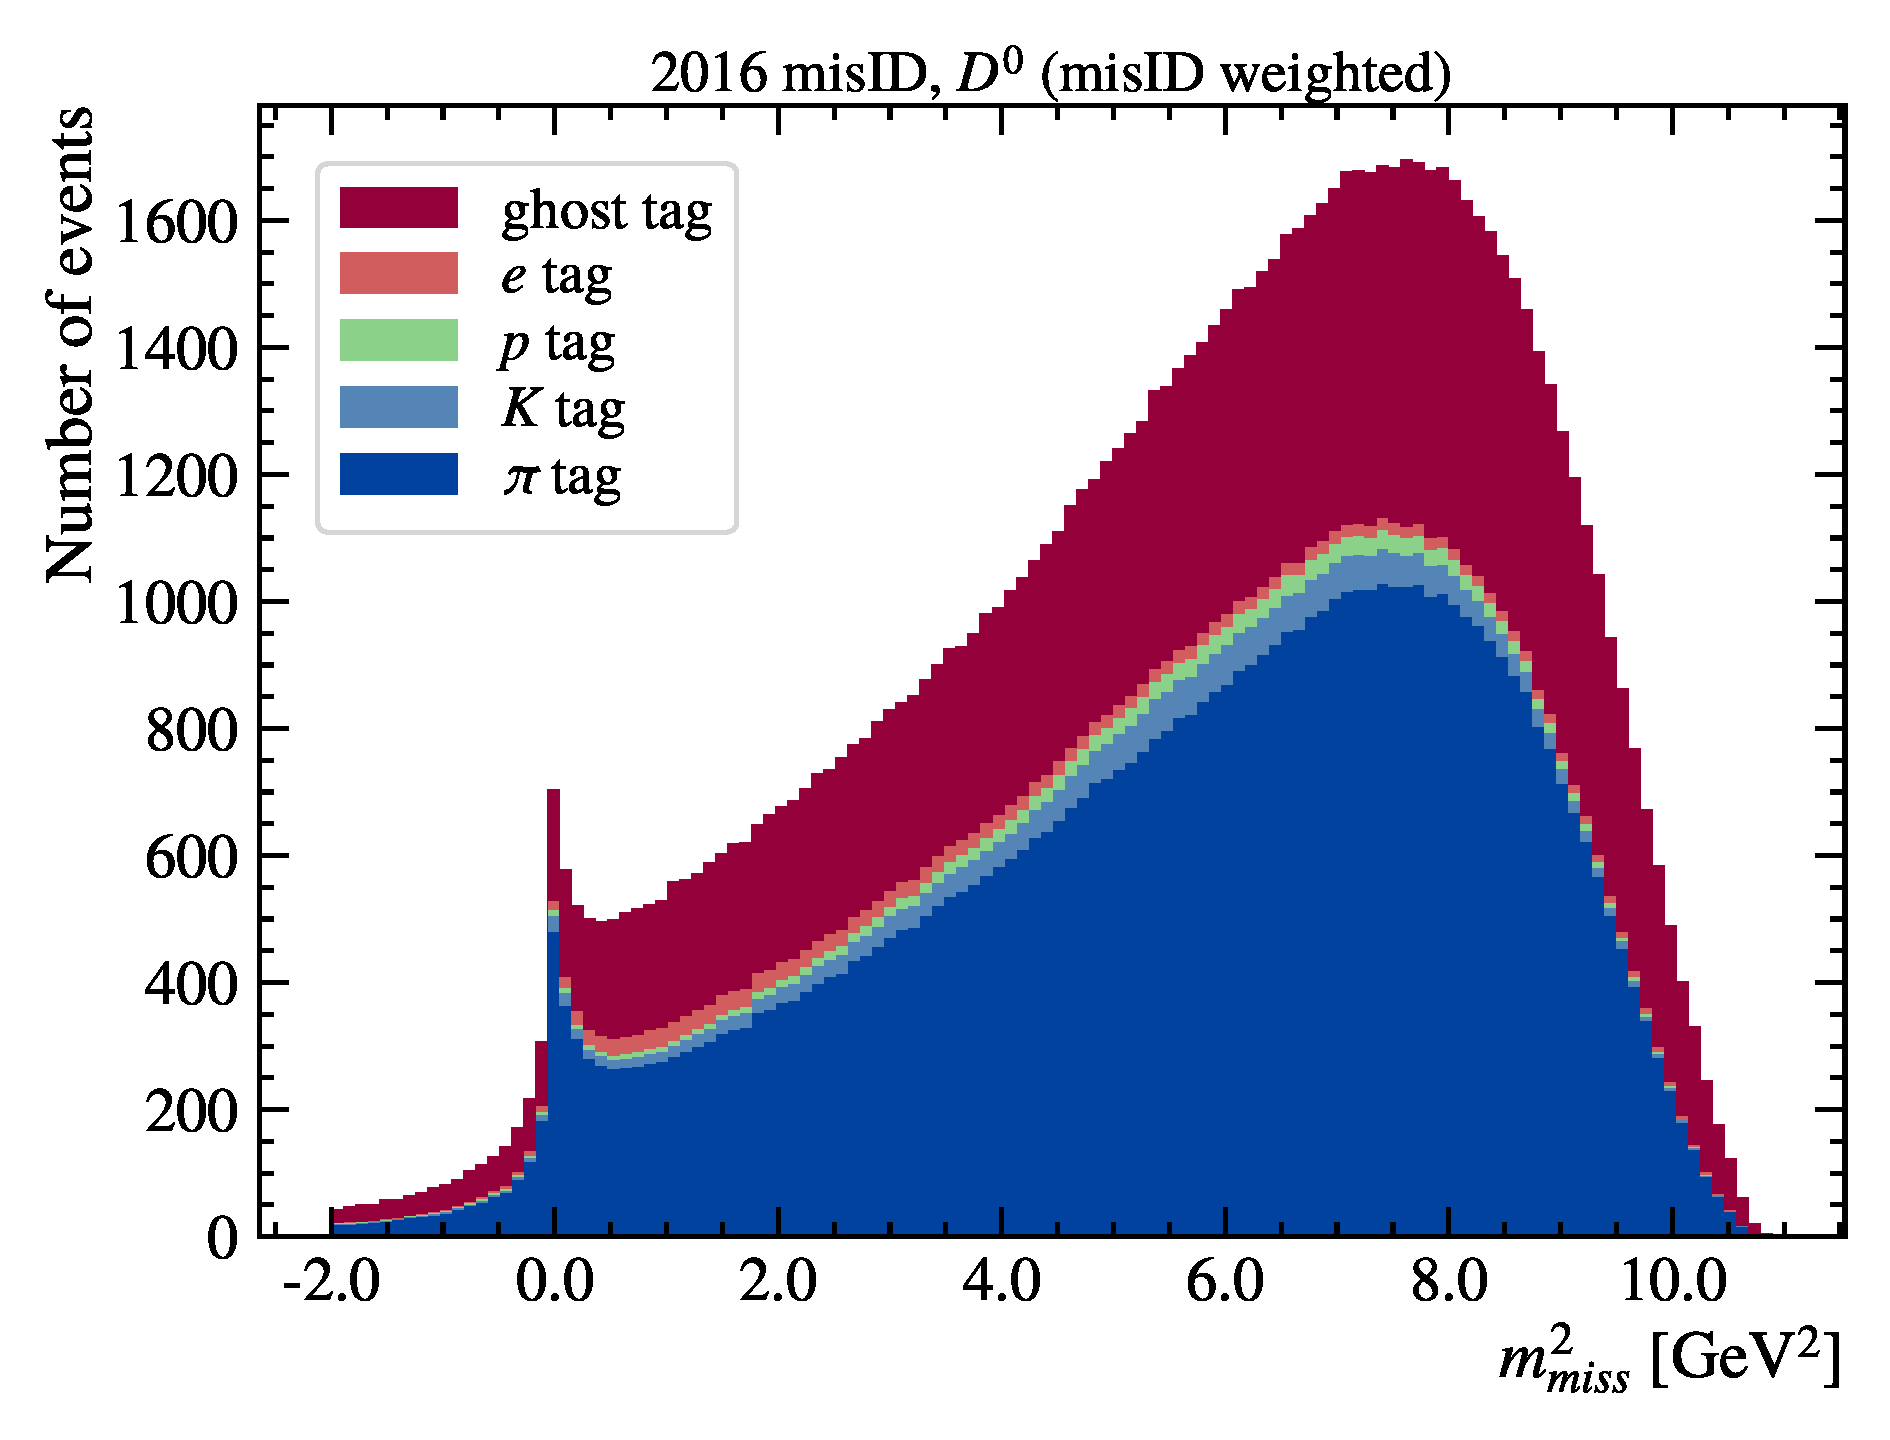
\includegraphics[width=\textwidth]{figs-fit-fit-templates/data-driven-plots/misid/D0_mm2.pdf}
    \end{subfigure}
    \hfill
    \begin{subfigure}[b]{0.32\textwidth}
        \centering
        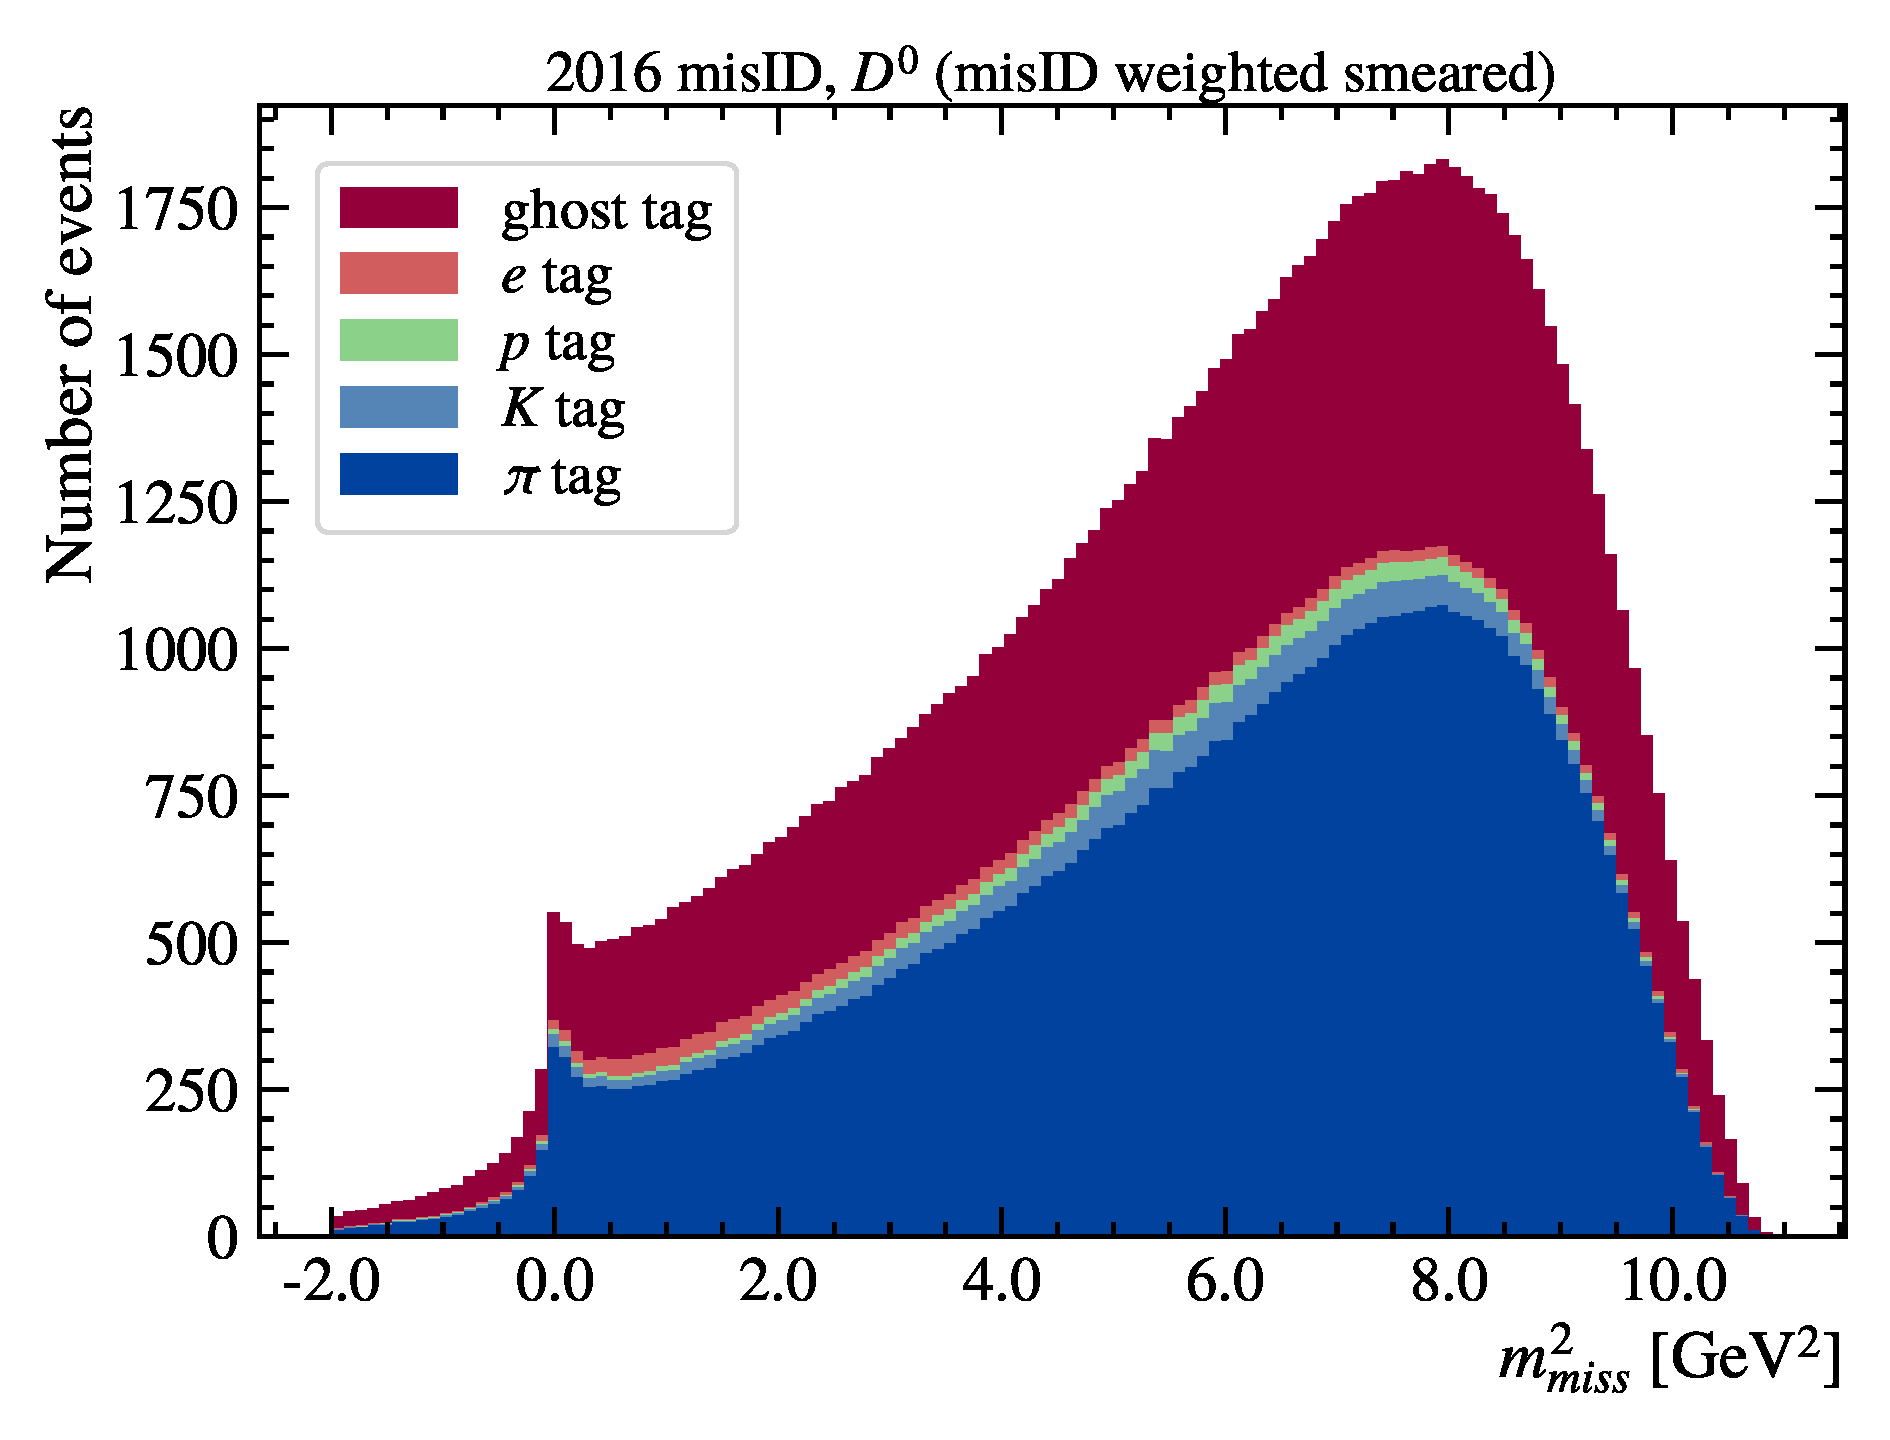
\includegraphics[width=\textwidth]{figs-fit-fit-templates/data-driven-plots/misid/D0_mm2_smr.pdf}
    \end{subfigure}
    \hfill
    \begin{subfigure}[b]{0.32\textwidth}
        \centering
        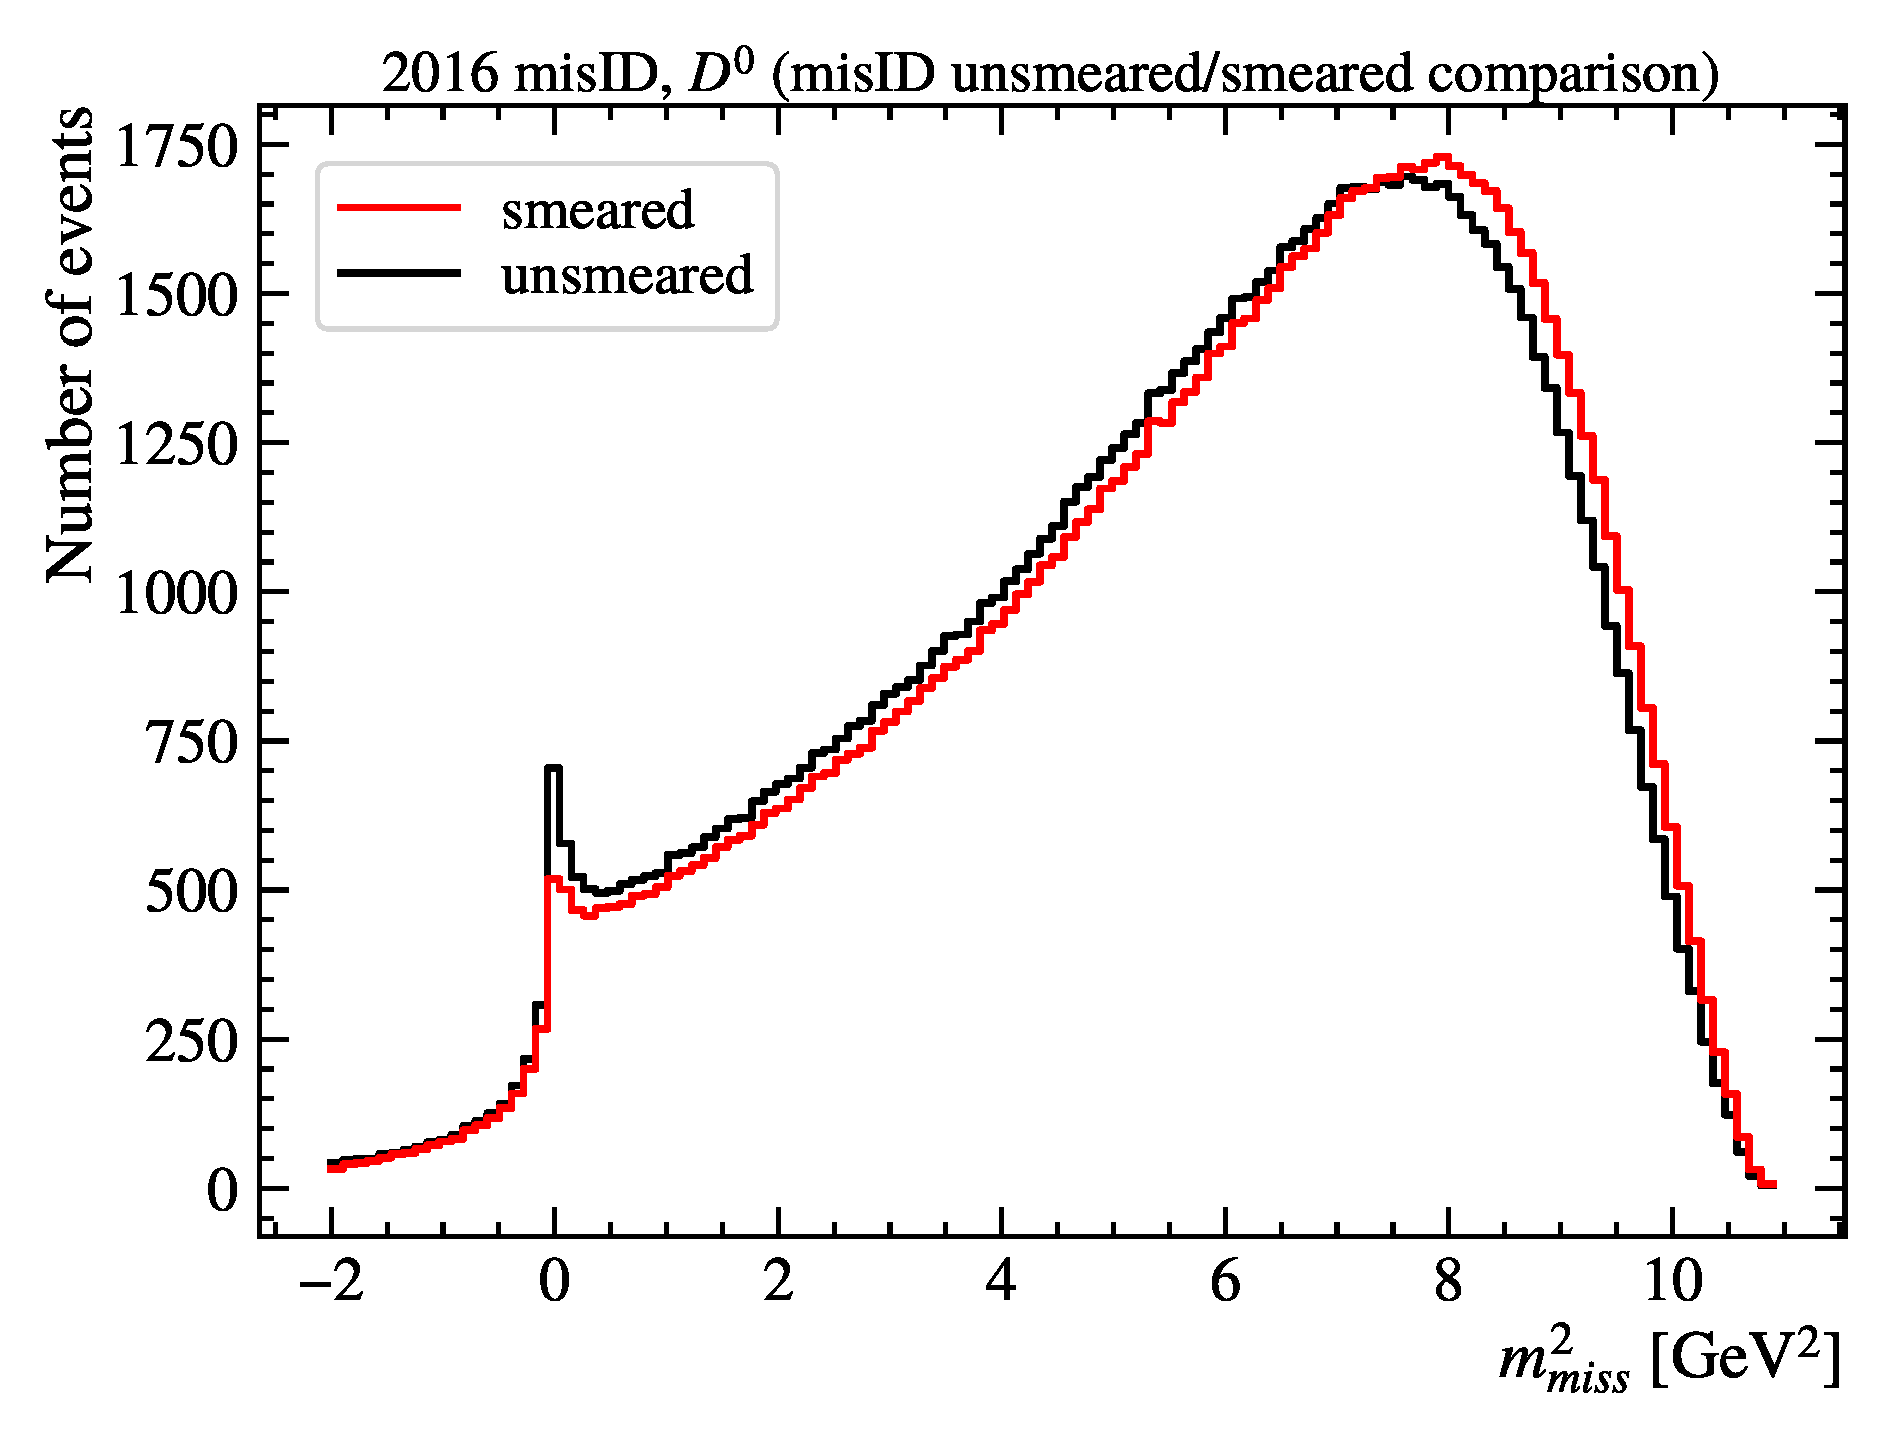
\includegraphics[width=\textwidth]{figs-fit-fit-templates/data-driven-plots/misid/D0_mm2_comp.pdf}
    \end{subfigure}
    \\
    \begin{subfigure}[b]{0.32\textwidth}
        \centering
        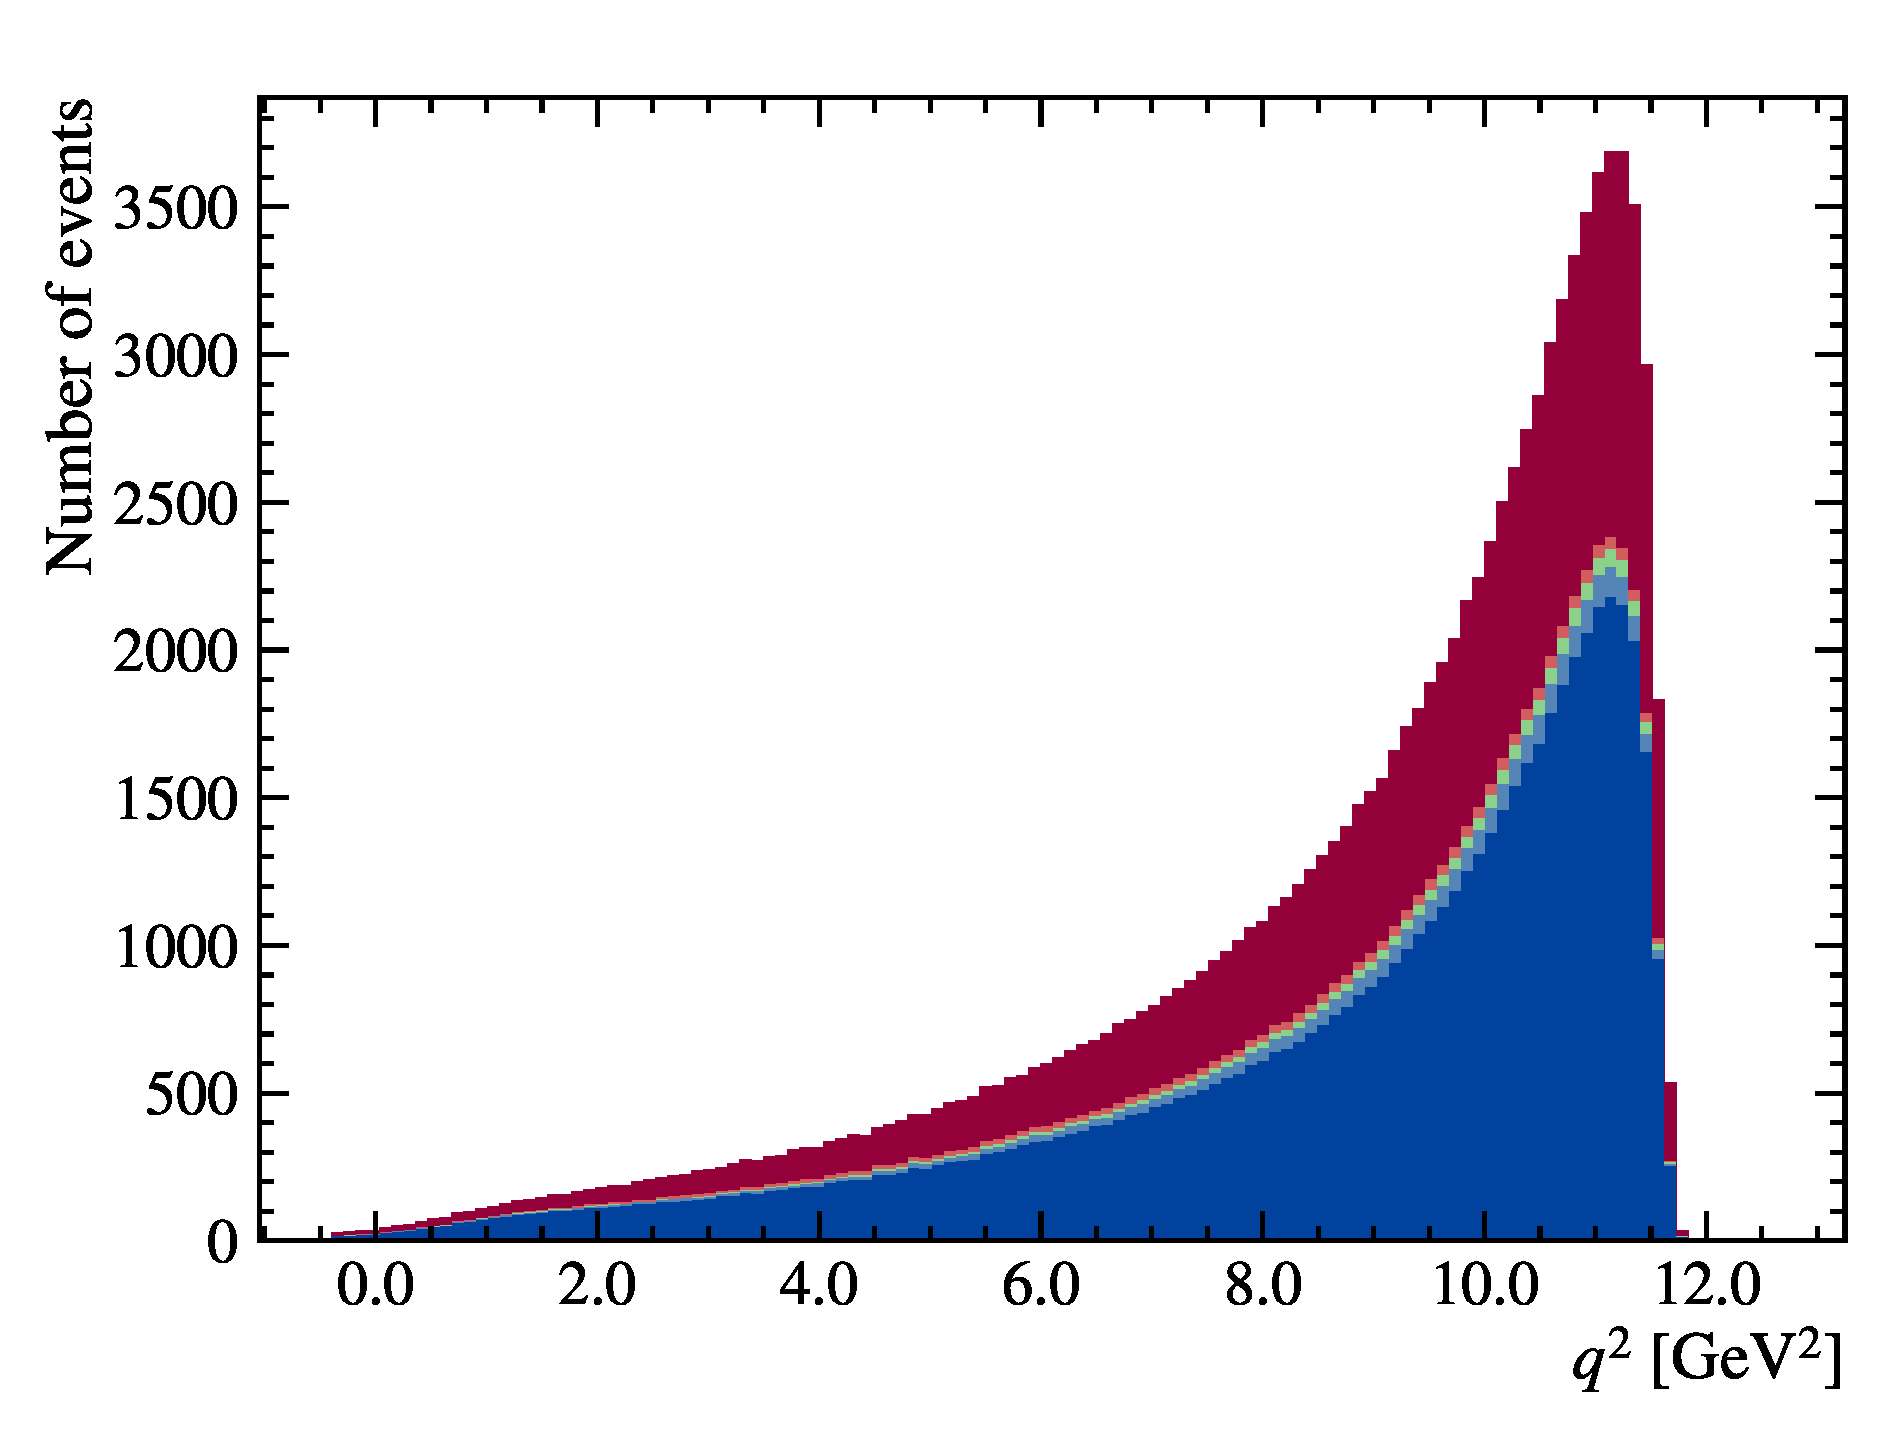
\includegraphics[width=\textwidth]{figs-fit-fit-templates/data-driven-plots/misid/D0_q2.pdf}
    \end{subfigure}
    \hfill
    \begin{subfigure}[b]{0.32\textwidth}
        \centering
        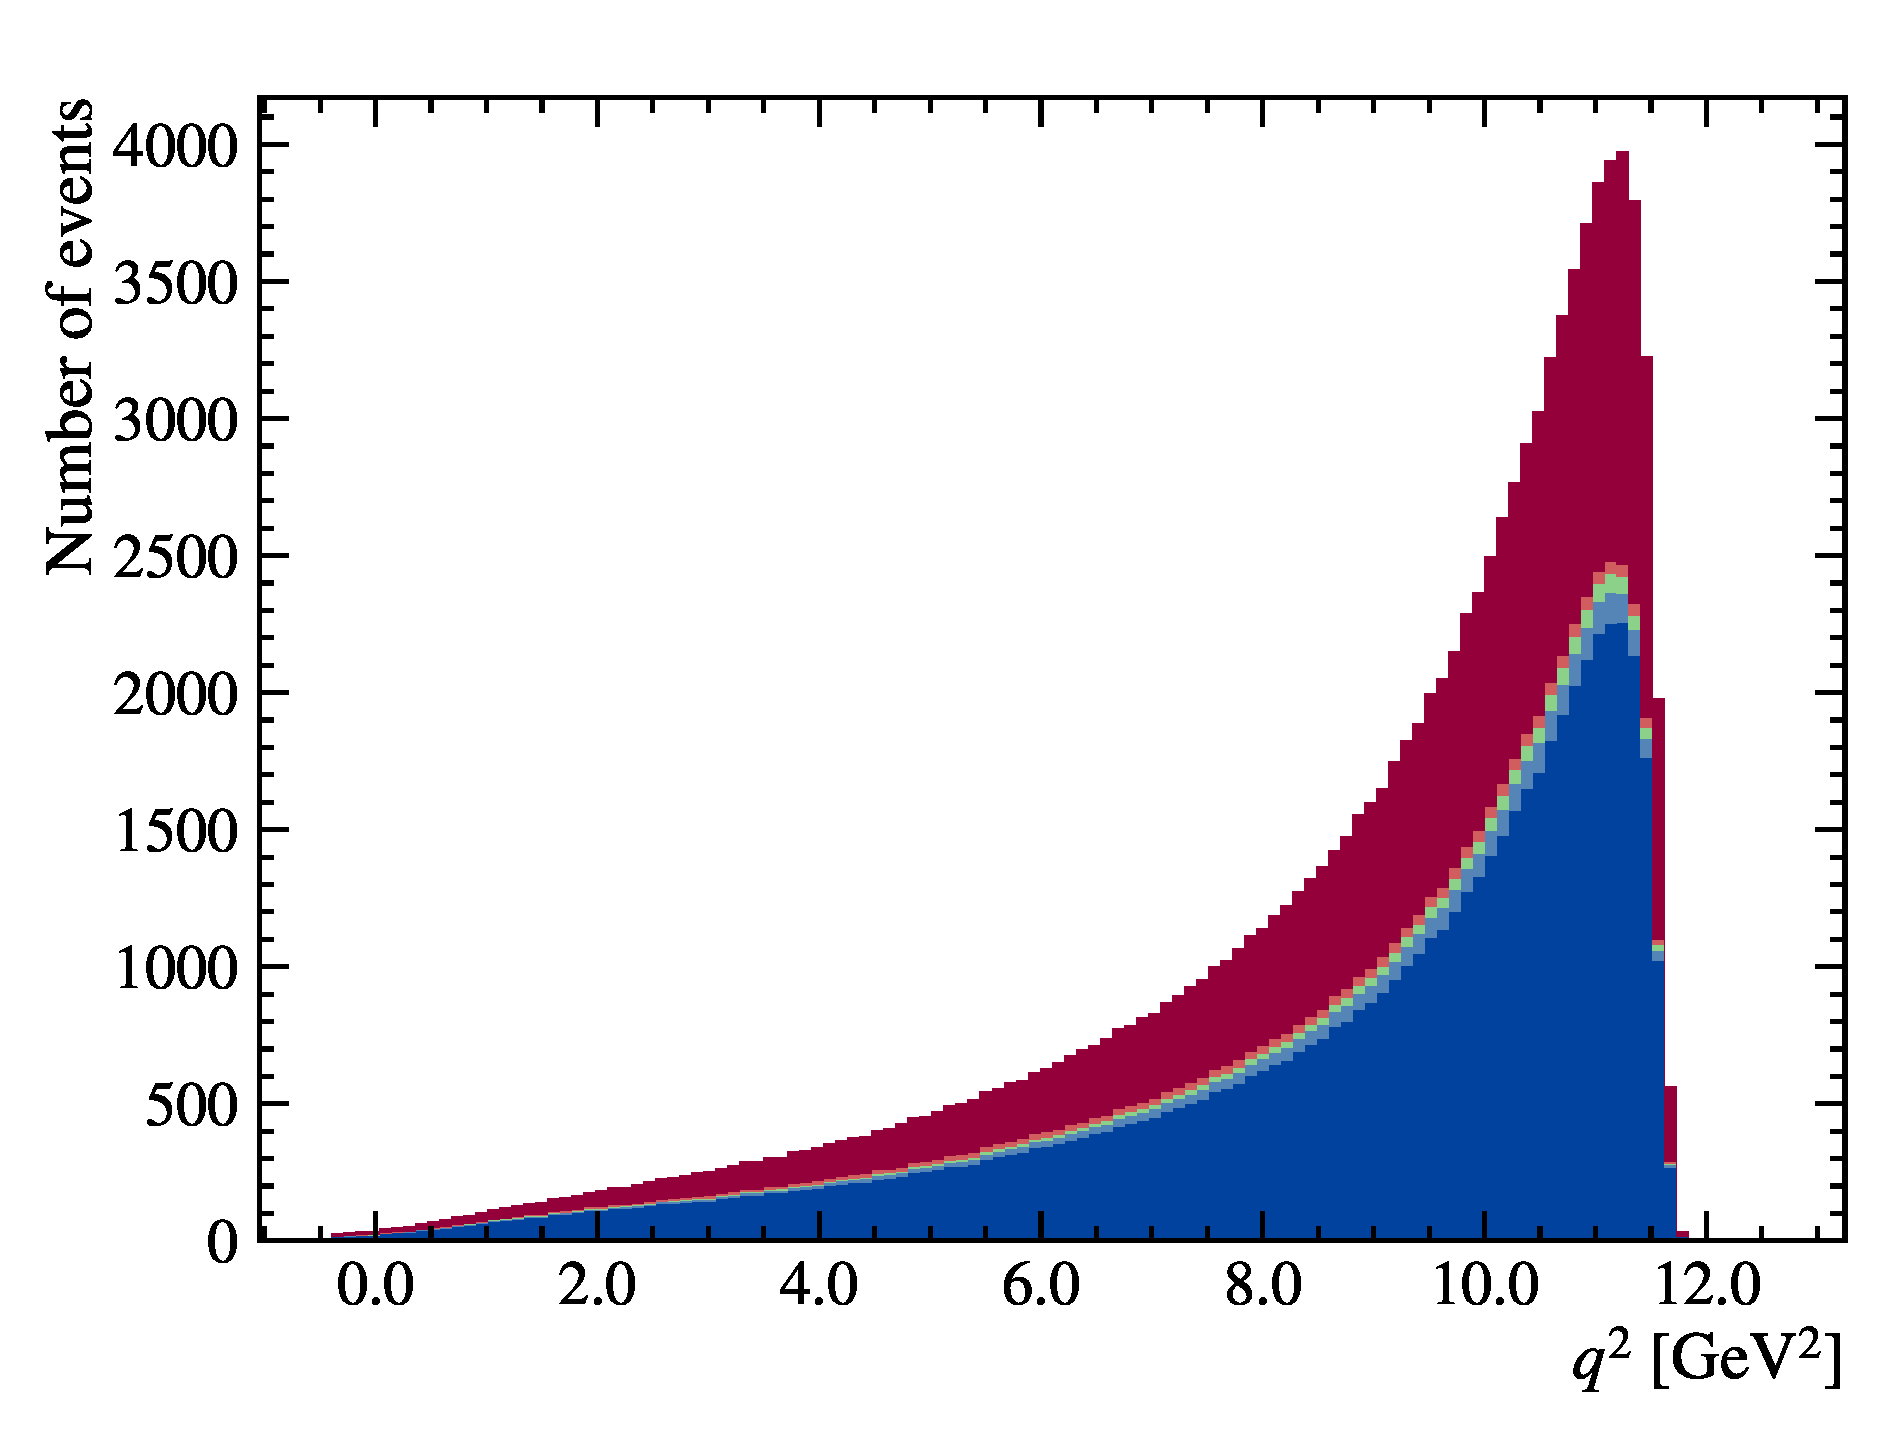
\includegraphics[width=\textwidth]{figs-fit-fit-templates/data-driven-plots/misid/D0_q2_smr.pdf}
    \end{subfigure}
    \hfill
    \begin{subfigure}[b]{0.32\textwidth}
        \centering
        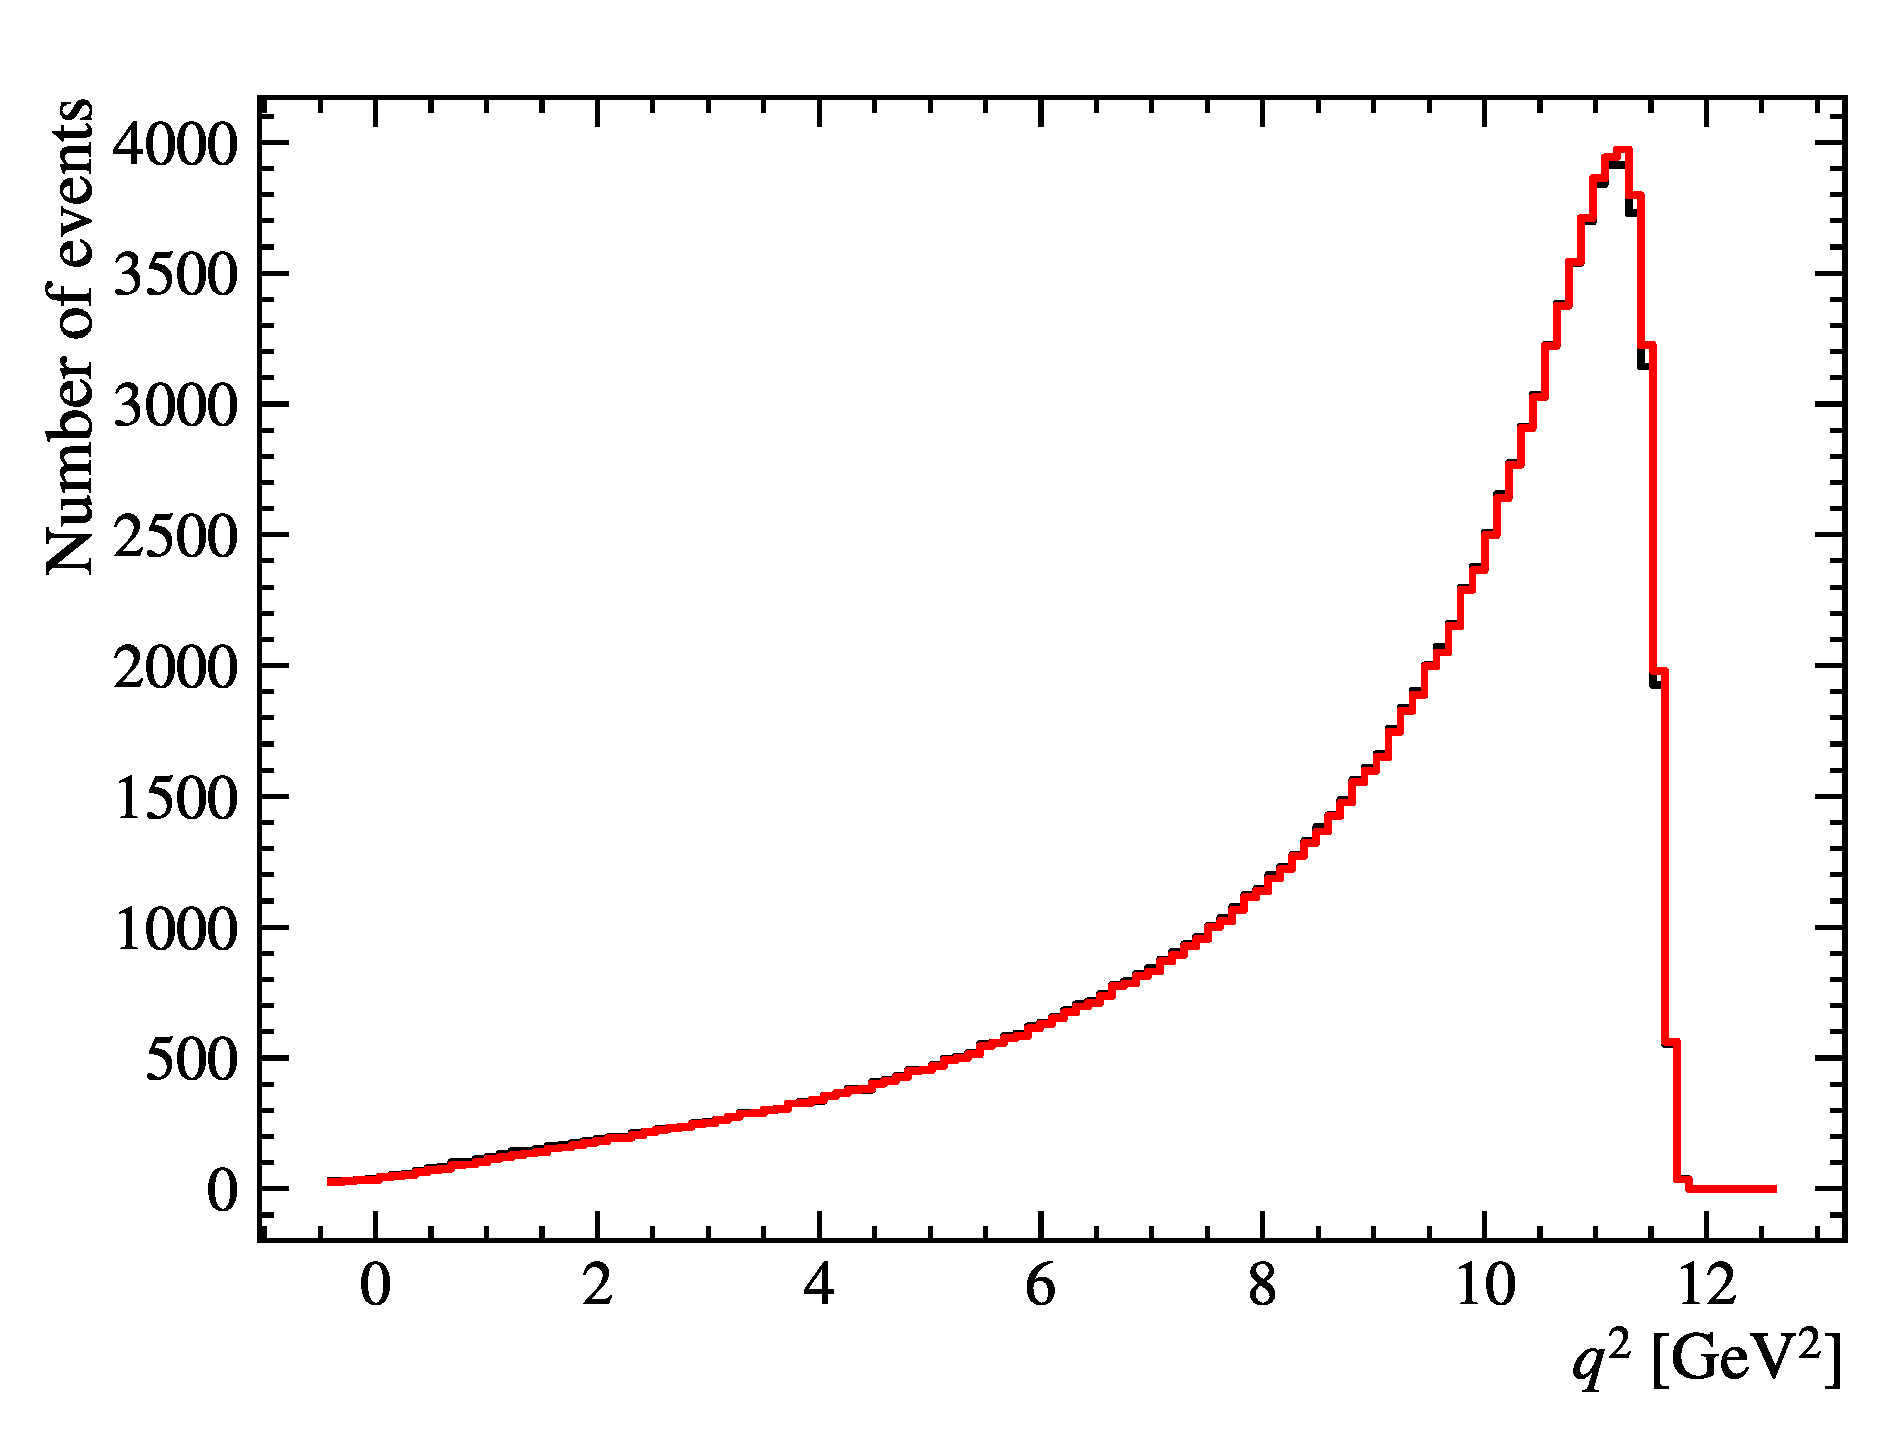
\includegraphics[width=\textwidth]{figs-fit-fit-templates/data-driven-plots/misid/D0_q2_comp.pdf}
    \end{subfigure}
    \\
    \begin{subfigure}[b]{0.32\textwidth}
        \centering
        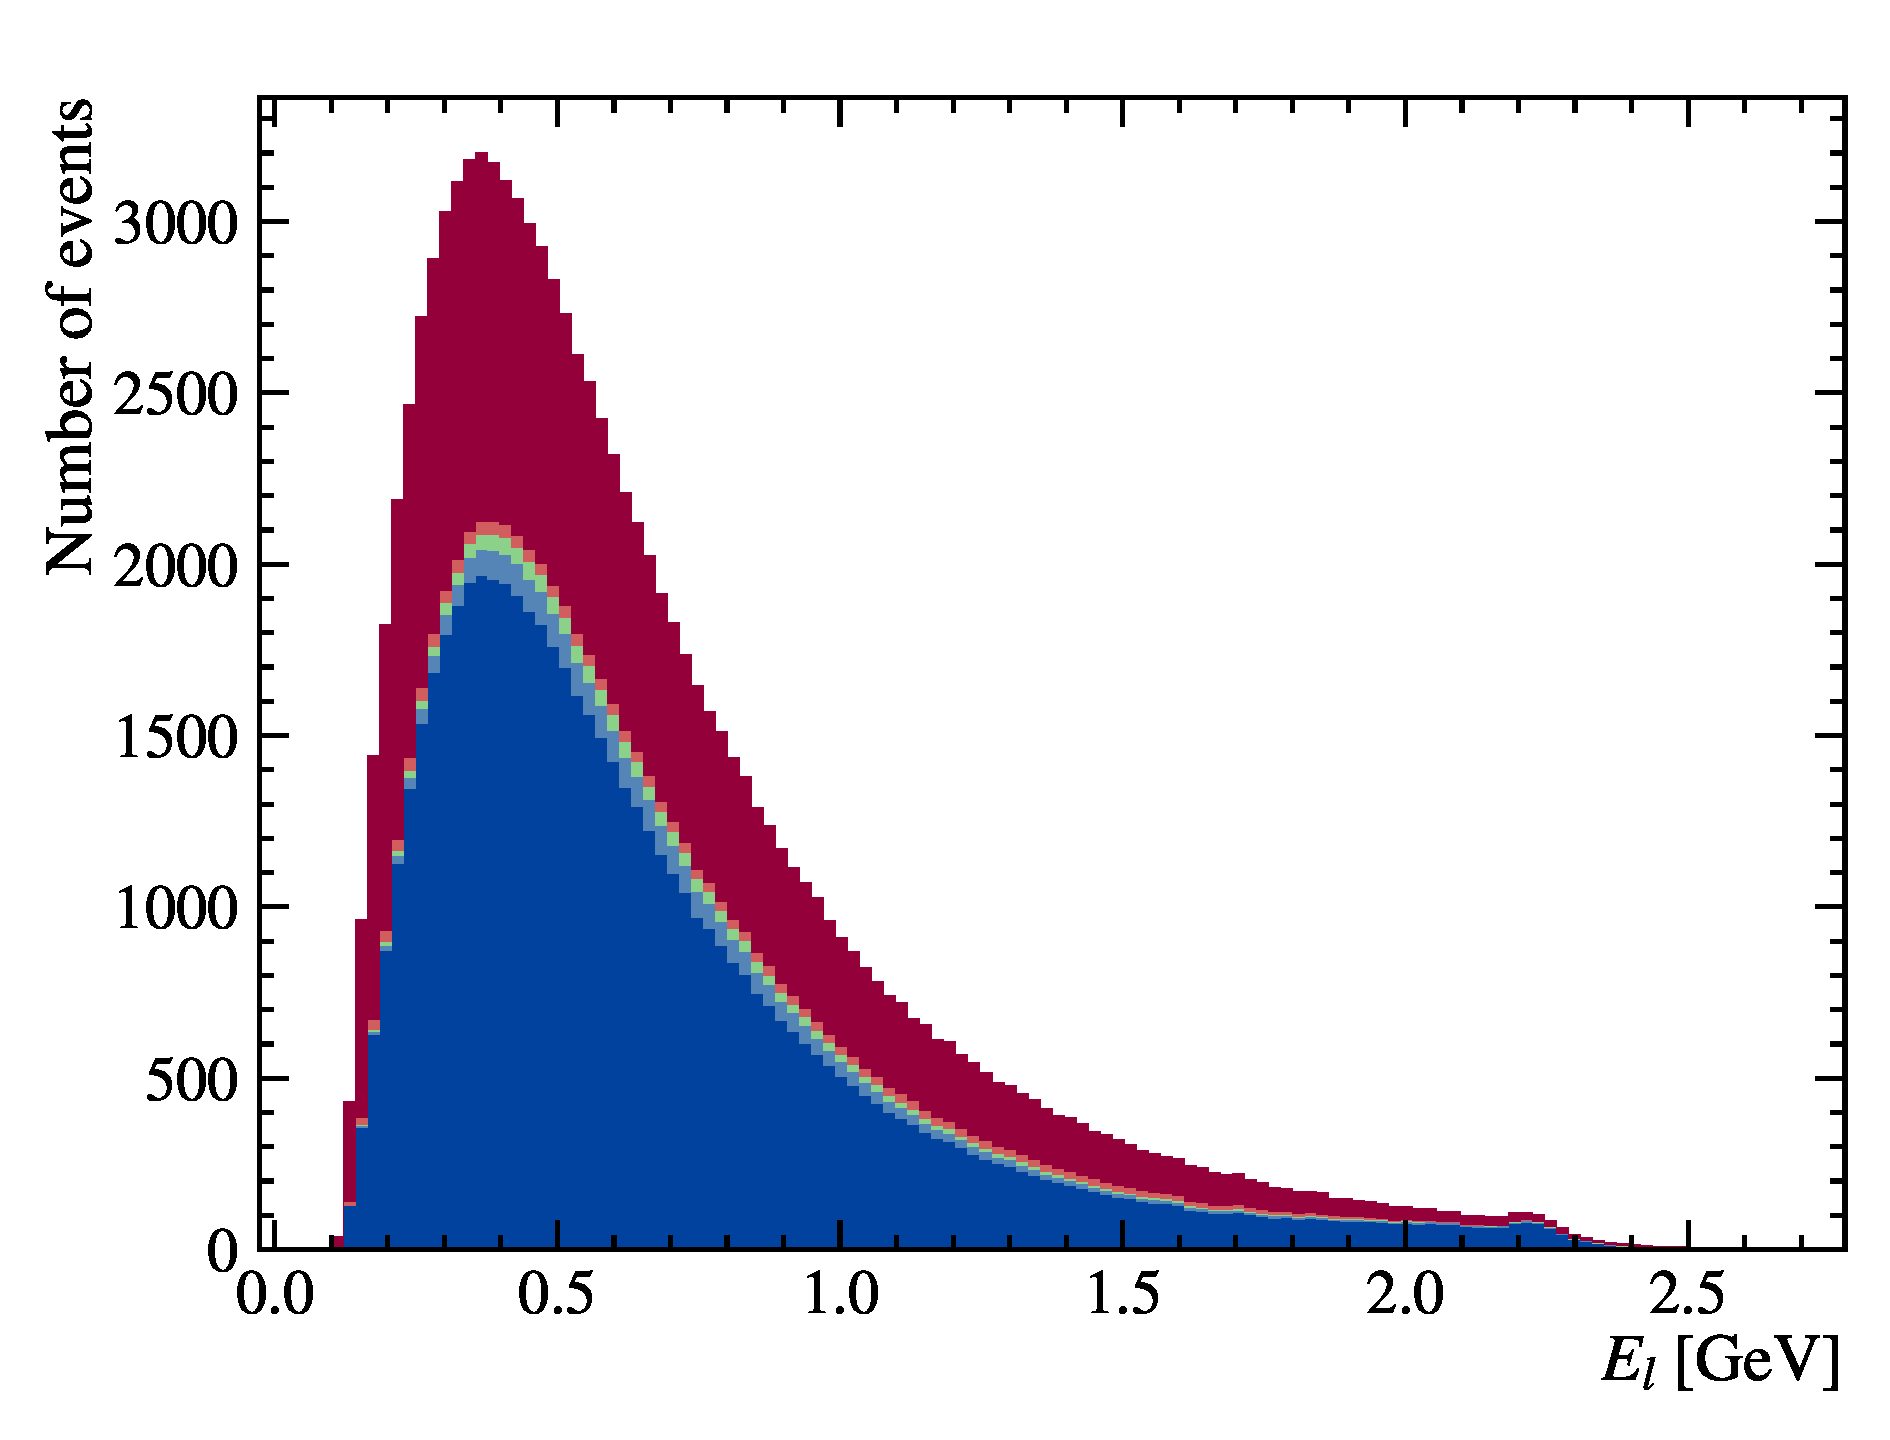
\includegraphics[width=\textwidth]{figs-fit-fit-templates/data-driven-plots/misid/D0_el.pdf}
    \end{subfigure}
    \hfill
    \begin{subfigure}[b]{0.32\textwidth}
        \centering
        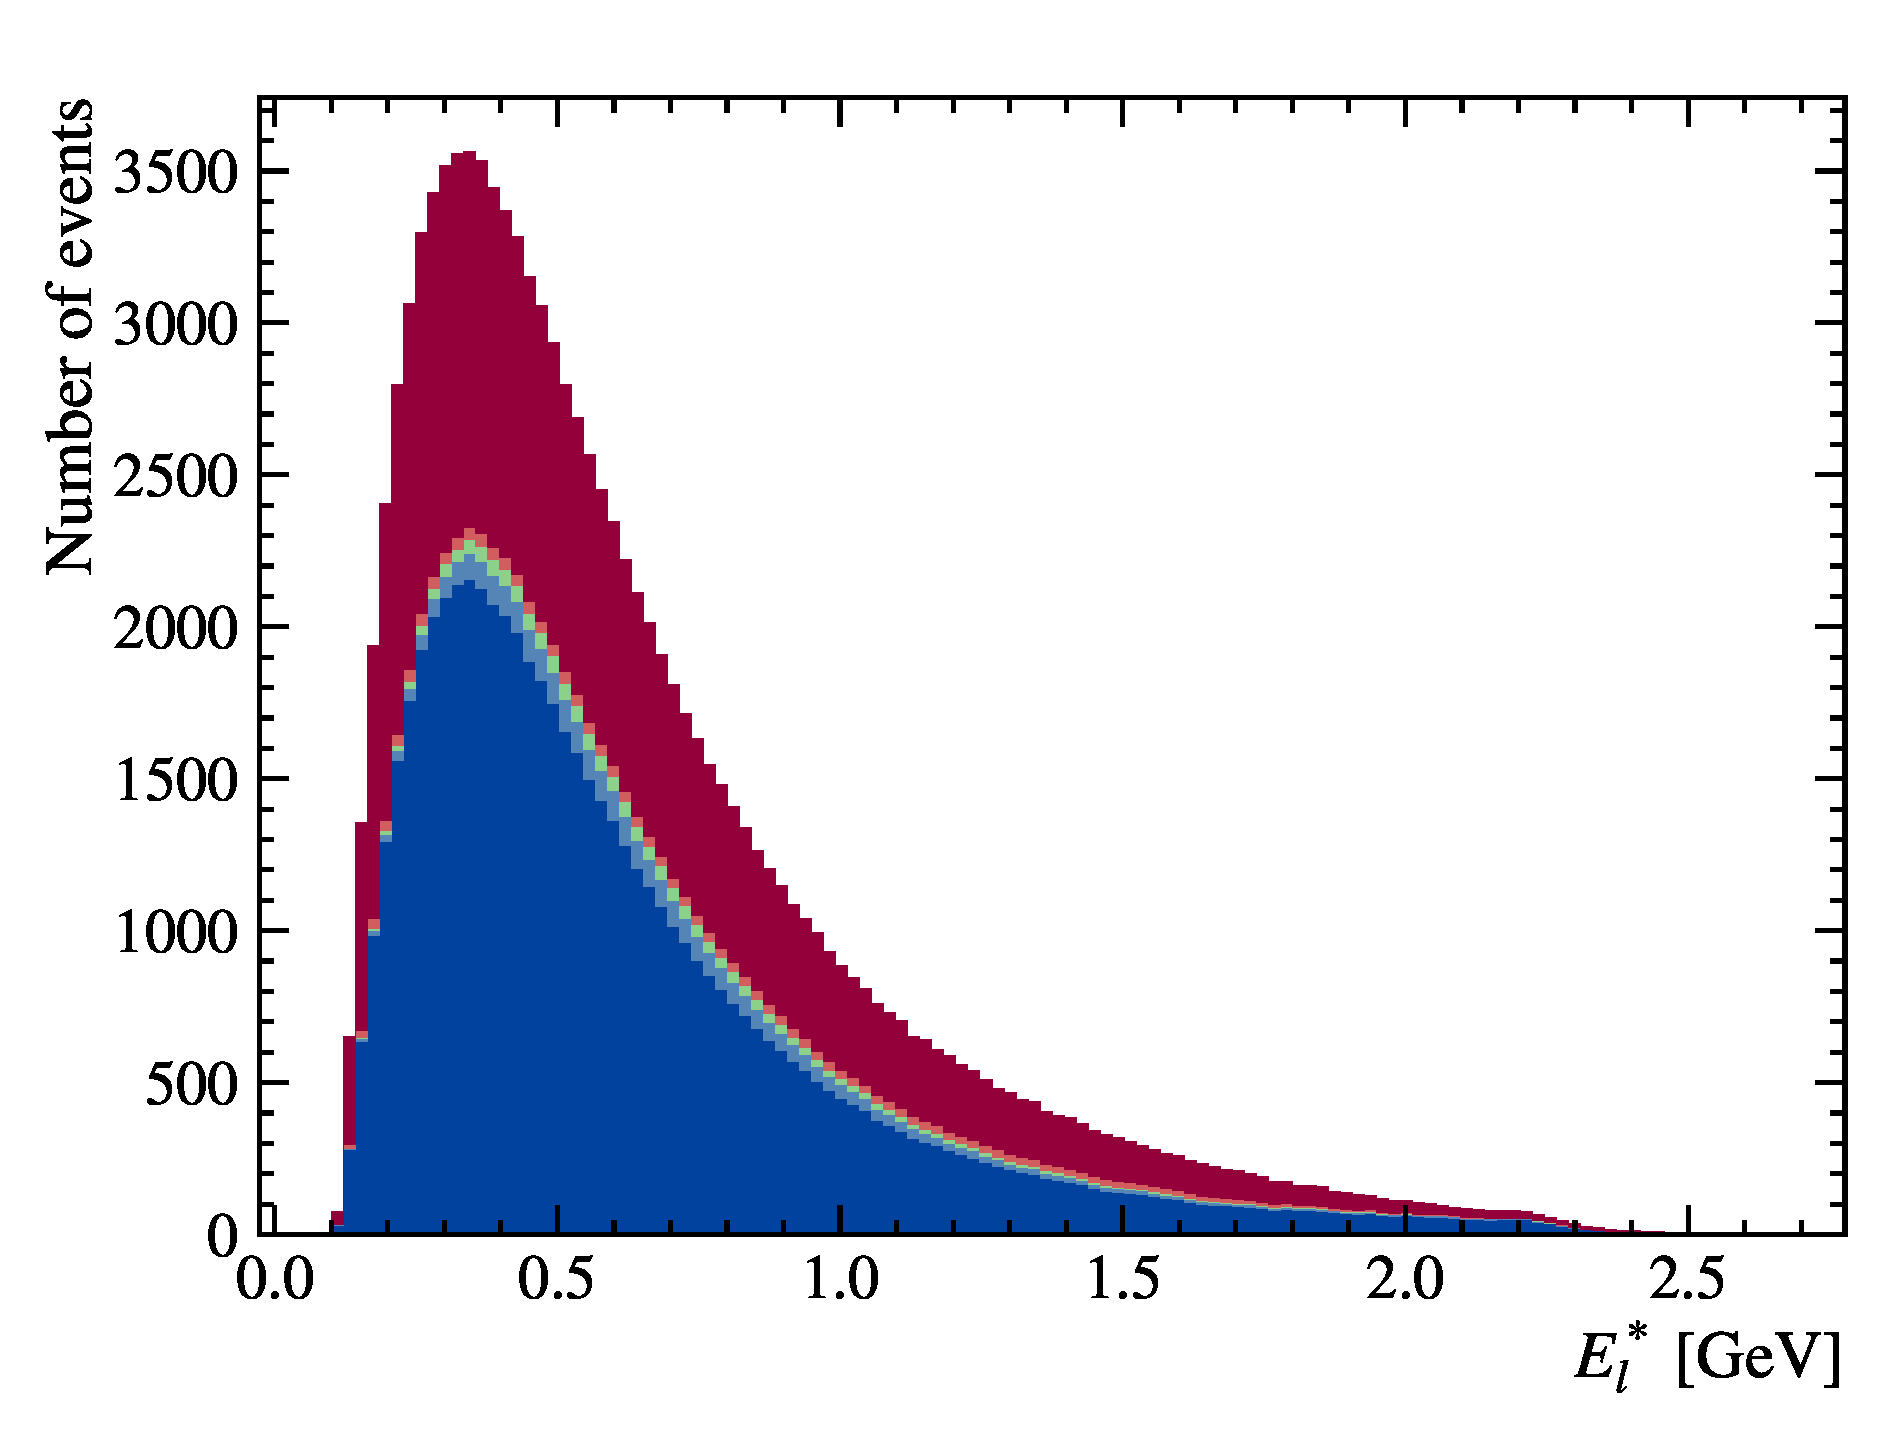
\includegraphics[width=\textwidth]{figs-fit-fit-templates/data-driven-plots/misid/D0_el_smr.pdf}
    \end{subfigure}
    \hfill
    \begin{subfigure}[b]{0.32\textwidth}
        \centering
        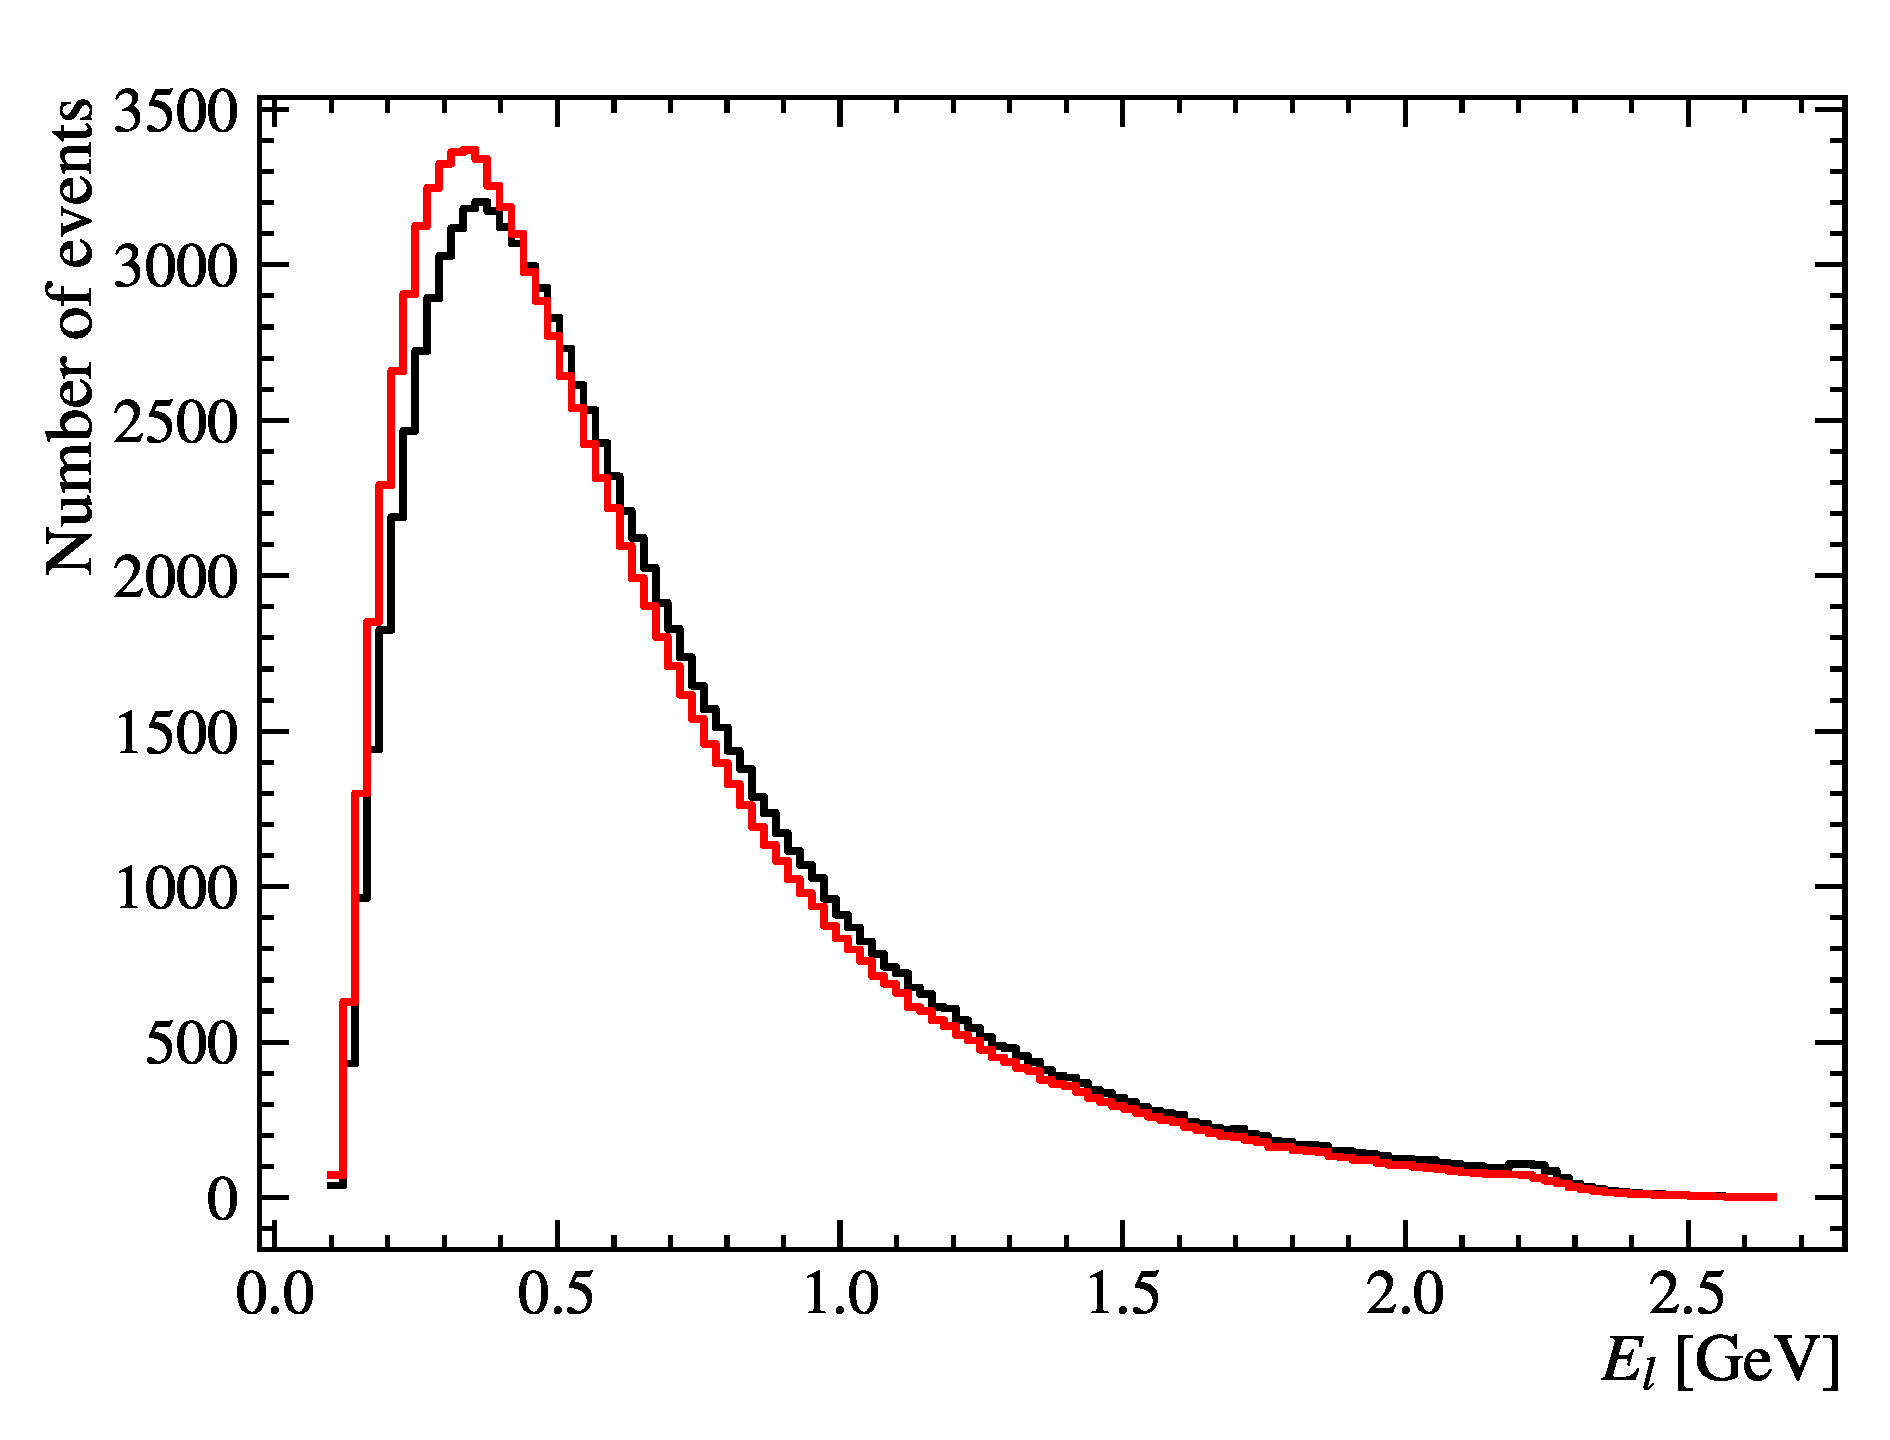
\includegraphics[width=\textwidth]{figs-fit-fit-templates/data-driven-plots/misid/D0_el_comp.pdf}
    \end{subfigure}
    \caption[Effect of DiF on fit variables]{
        Effect of DiF on fit variables.

        The plots displayed here are contributions of 2016 $D^0$ misID control
        samples ($B^- \rightarrow D^0 t^-$) to the fit variables.

        The first column is unsmeared misID fit variables \mmSq, \qSq, \el; the
        second column smeared; the third column comparison between the overall
        shape of unsmeared/smeared fit variables. \\
        Note that the total number of events is not guaranteed to be conserved,
        because smearing may put fit variables outside of the
        acceptance range.
    }
    \label{fig:unfolding-fit-vars-smear}
\end{figure}

\section{Fit results}
\label{ref:fit:results}

The fitted yields are grouped as follows:
\Dz\muon, \Dstarp\muon, \Dstarz\muon,
signal,
misID,
combinatorial backgrounds,
four $1P$ $D^{**}$,
$D^{**}$ heavy,
$DD$,
and $D_s$.
The combined yields of the groups of the signal fit are reported in
\cref{tab:fit-yields} for both fit channels,
with the signal yields blinded (replaced with a random number).

\begin{table}[!ht]
    \centering
    \caption{Fitted yields of the signal fit.}
    \label{tab:fit-yields}

\begin{subtable}[b]{0.5\textwidth}
    \centering

\begin{tabular}[b]{lr}
\hline
 Group               &    Yields \\
\hline
 norm. ($D^0\mu$)    &   445,095 \\
 norm. ($D^{*+}\mu$) &   115,124 \\
 norm. ($D^{*0}\mu$) & 1,176,363 \\
 sig. (random)       &        14 \\
 $D^{**}$            &   167,968 \\
 $D^{**}$ heavy      &    38,147 \\
 $D_s$               &     5,285 \\
 $DD$                &    96,236 \\
 comb. bkg.          &    20,596 \\
 misID               &    56,596 \\
\hline
\end{tabular}

    \caption{\Dz channel}
\end{subtable}%
%%%%
\begin{subtable}[b]{0.5\textwidth}
    \centering

\begin{tabular}[b]{lr}
\hline
 Group               &   Yields \\
\hline
 norm. ($D^{*+}\mu$) &  427,783 \\
 sig. (random)       &        5 \\
 $D^{**}$            &   37,181 \\
 $D^{**}$ heavy      &   12,804 \\
 $D_s$               &    3,730 \\
 $DD$                &   33,588 \\
 comb. bkg.          &   16,906 \\
 misID               &    8,175 \\
\hline
\end{tabular}

    \caption{\Dstar channel}
\end{subtable}

\end{table}


The pre-control fit results are plotted in \cref{appx:suppl:fit-pre-ctrl};
the control fit results are displayed in
\cref{fig:ctrl-1os-d0,fig:ctrl-2os-d0,fig:ctrl-dd-d0} for \Dz channel;
\cref{fig:ctrl-1os-dst,fig:ctrl-2os-dst,fig:ctrl-dd-dst} for \Dstar channel;
the signal fit results in \cref{fig:sig-d0,fig:sig-dst}
for the \Dz and \Dstar channel, accordingly.


% ctrl
\begin{figure}[!htb]
    \centering
    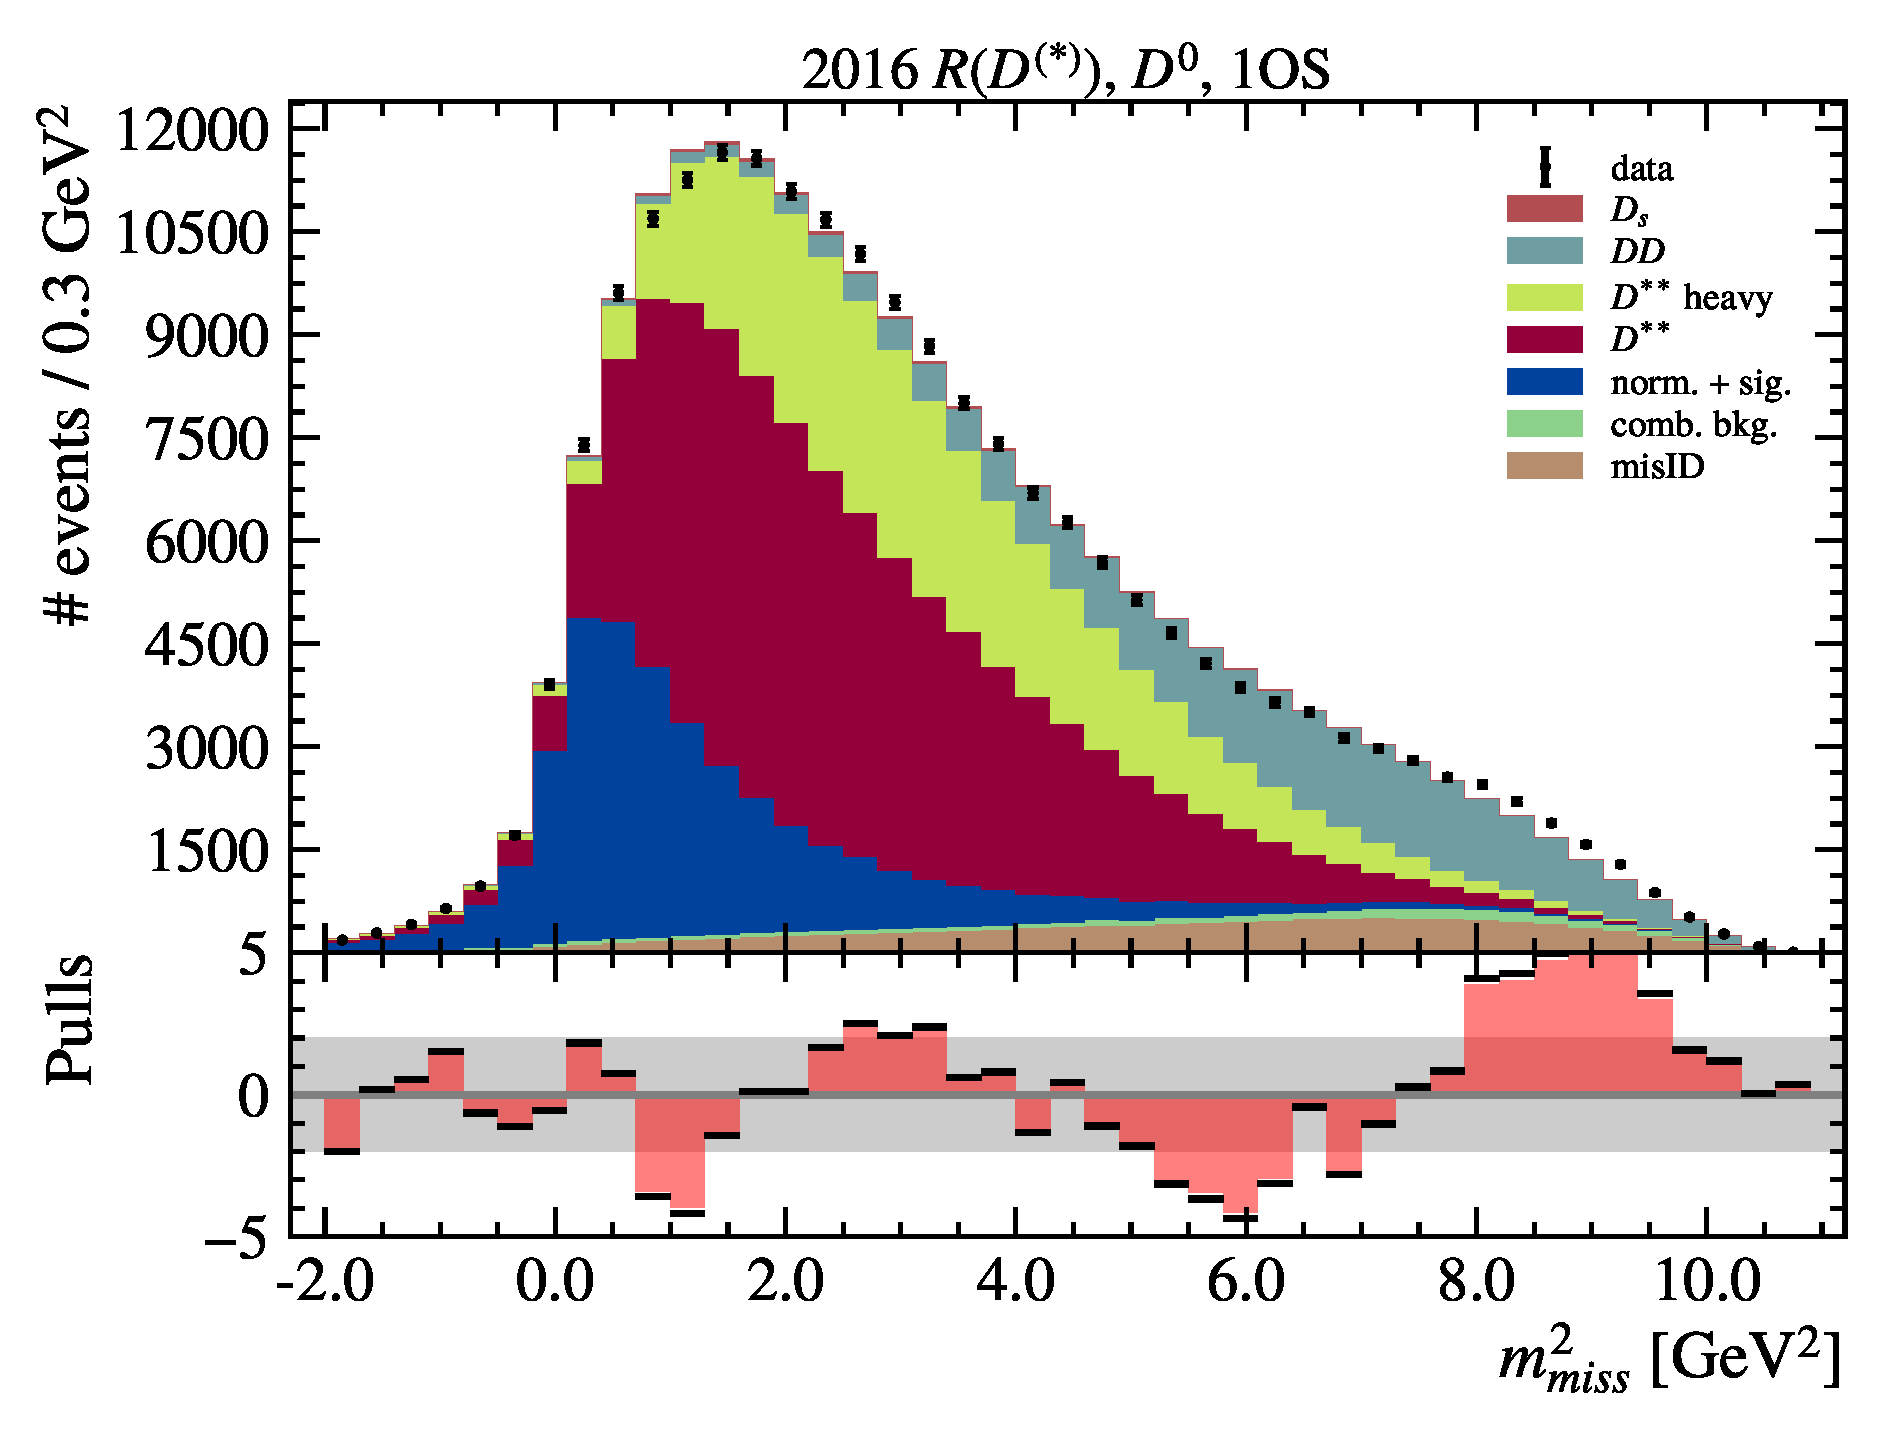
\includegraphics[width=0.32\textwidth]{./figs-fit-fit-results/ctrl-fit/stacked/fit_result-stacked-D0-1os-mmiss2.pdf}
    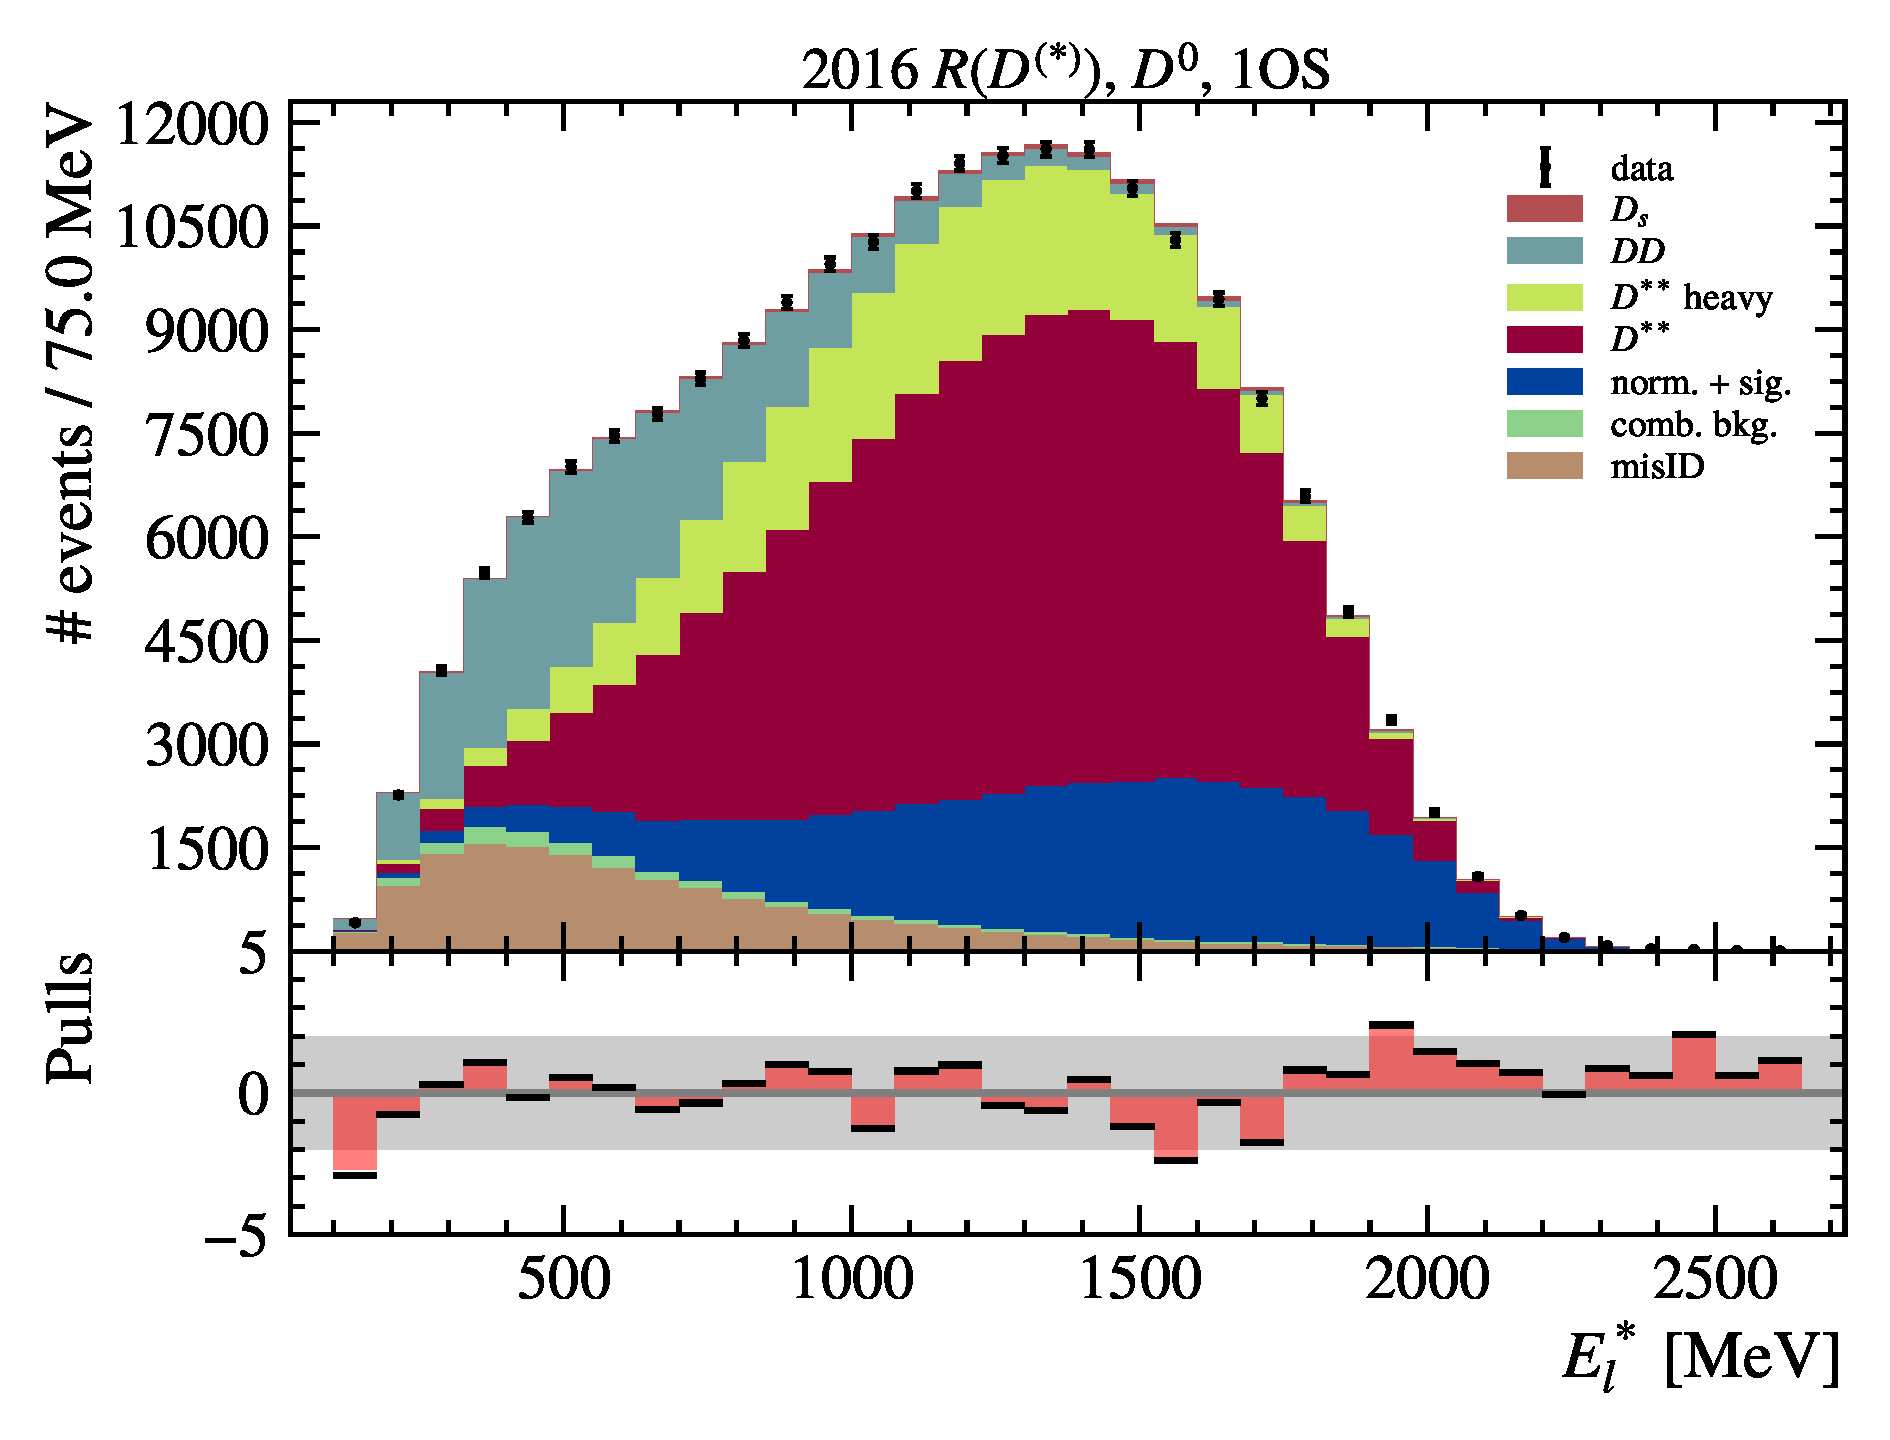
\includegraphics[width=0.32\textwidth]{./figs-fit-fit-results/ctrl-fit/stacked/fit_result-stacked-D0-1os-el.pdf}
    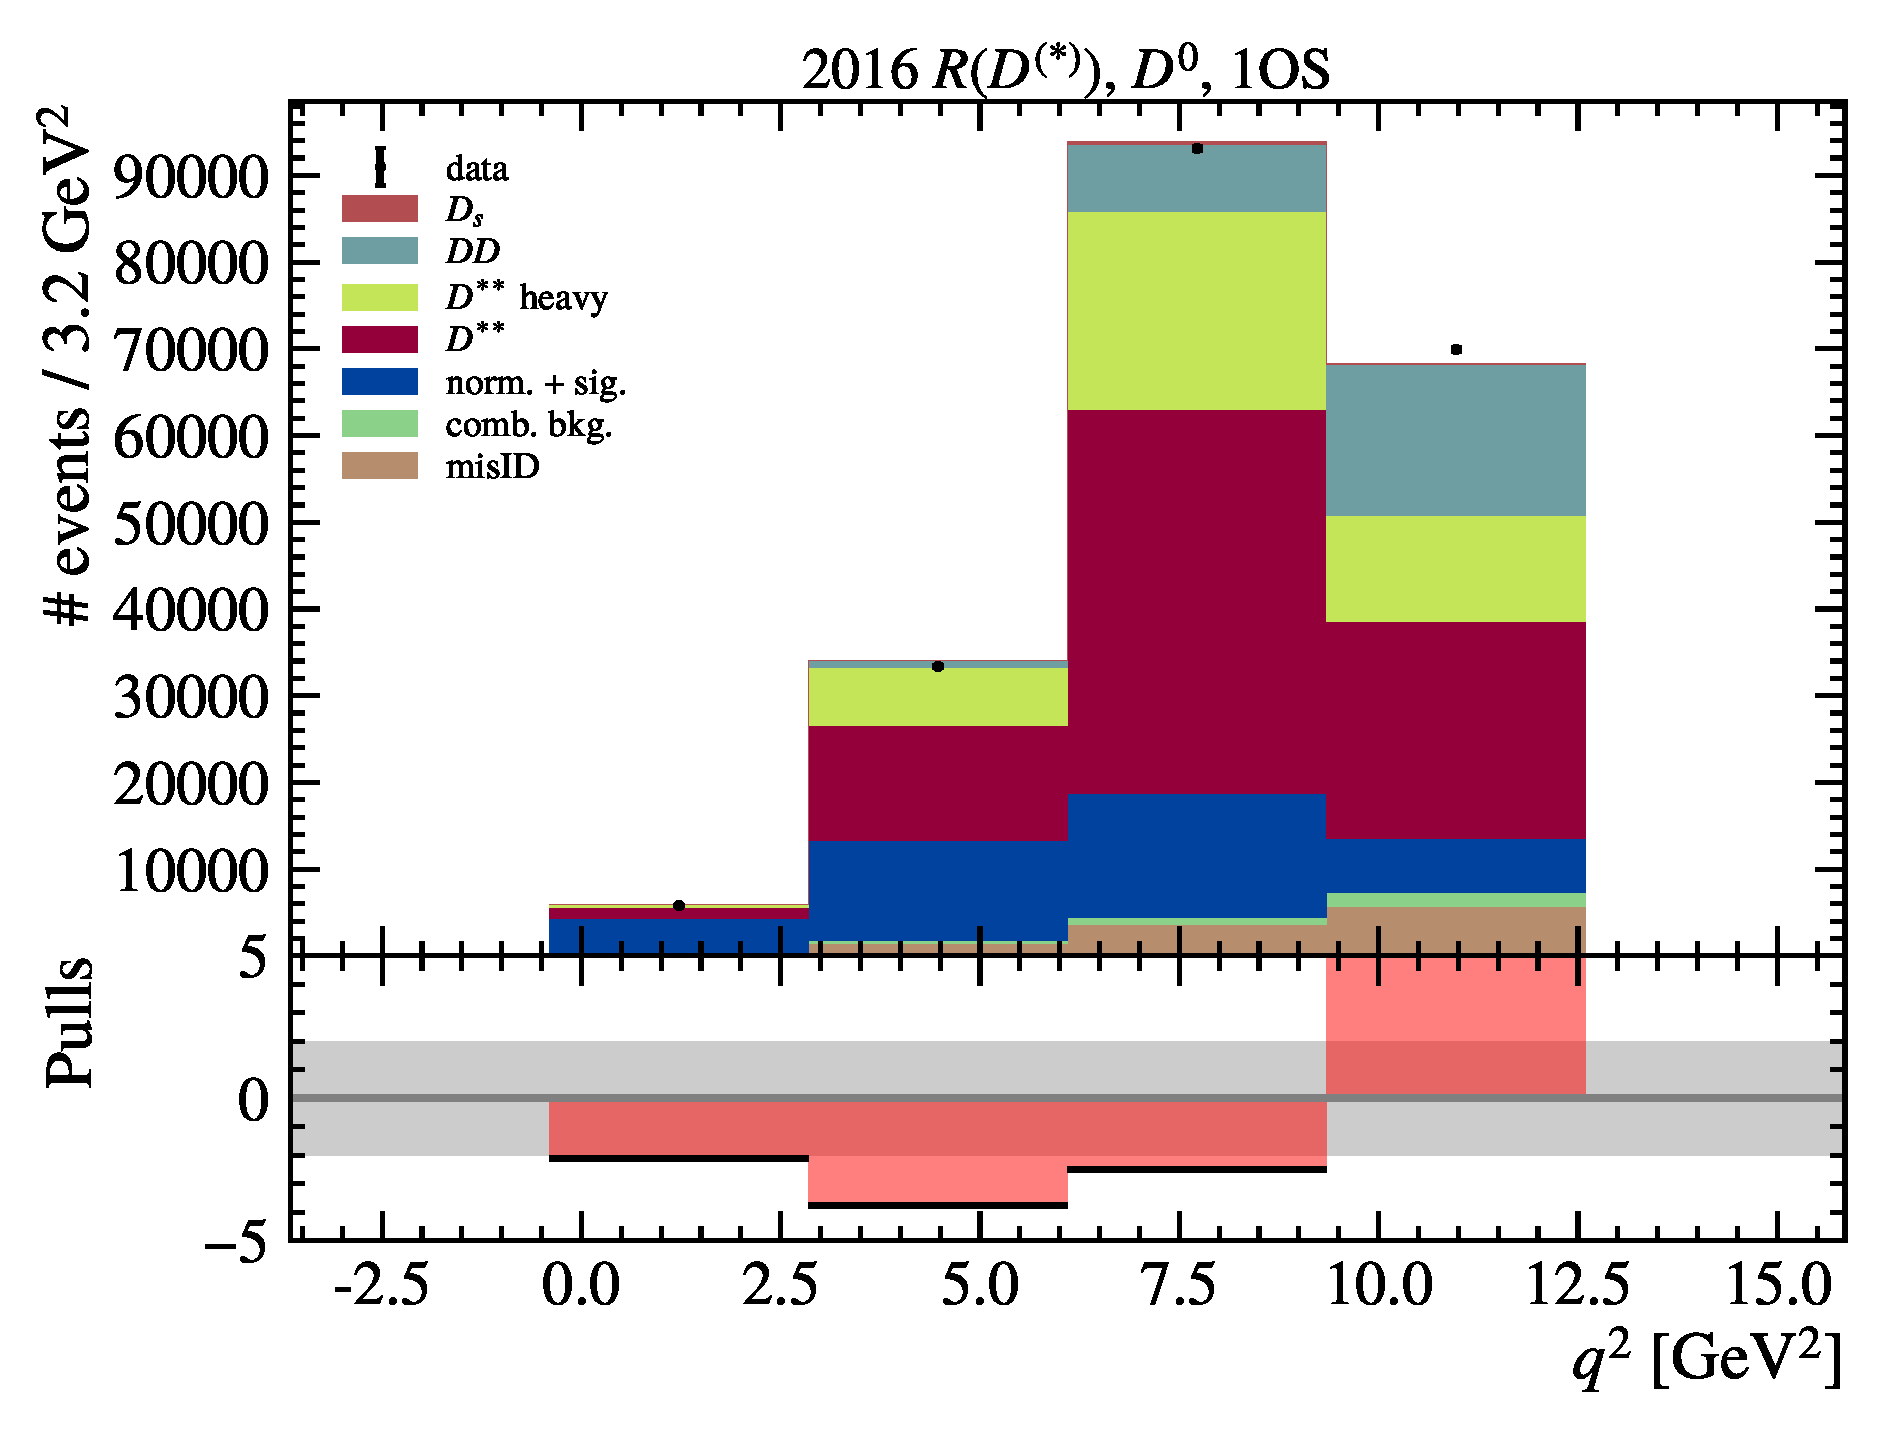
\includegraphics[width=0.32\textwidth]{./figs-fit-fit-results/ctrl-fit/stacked/fit_result-stacked-D0-1os-q2.pdf}

    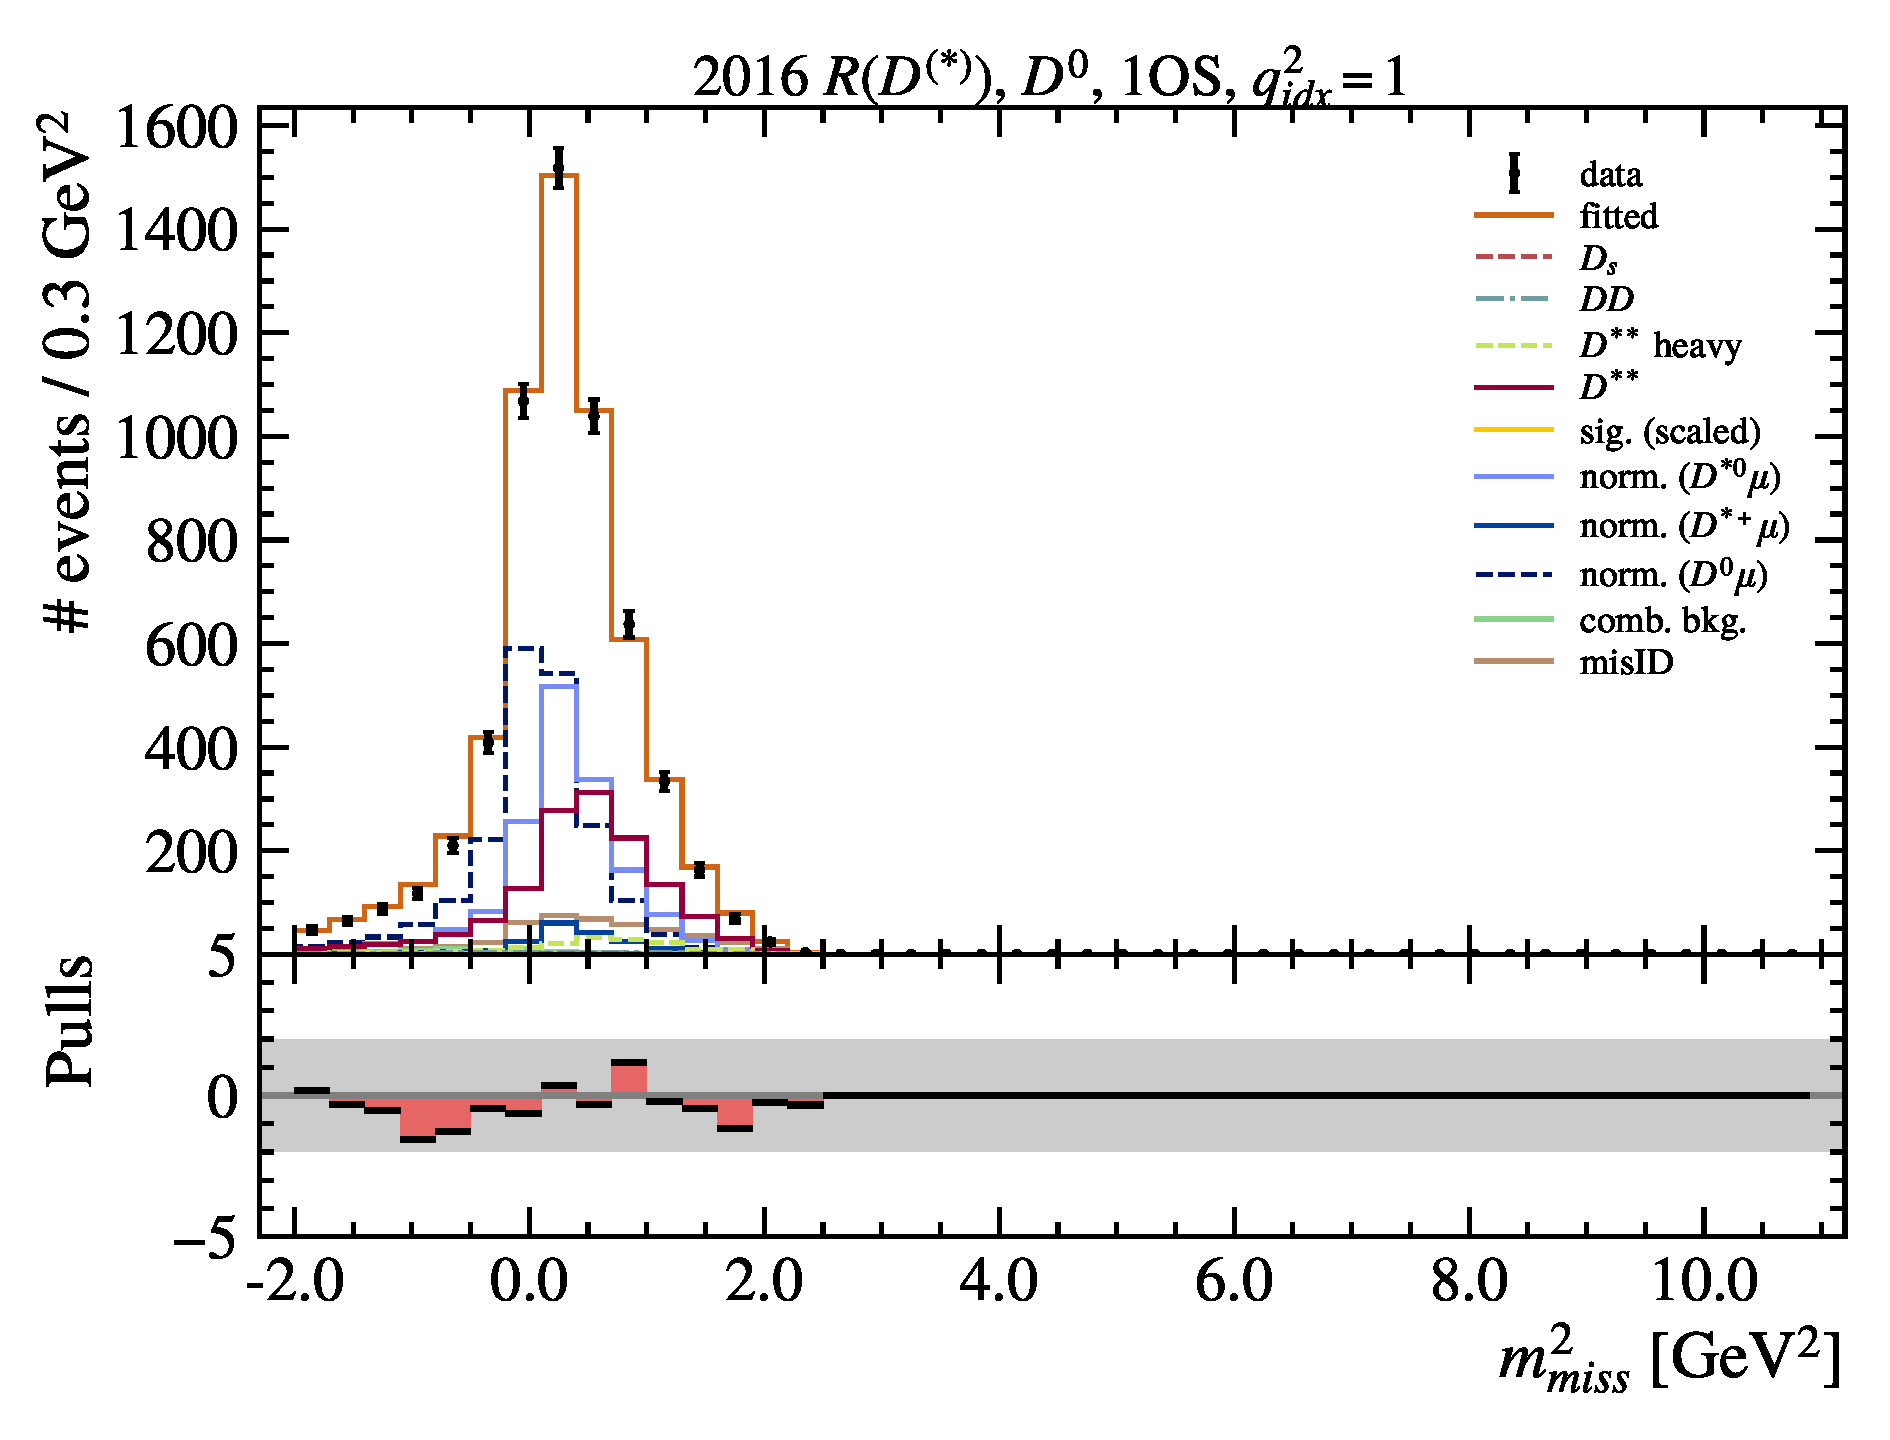
\includegraphics[width=0.24\textwidth]{./figs-fit-fit-results/ctrl-fit/lines_q2_slices/fit_result-lines_q2_idx1-D0-1os-mmiss2.pdf}
    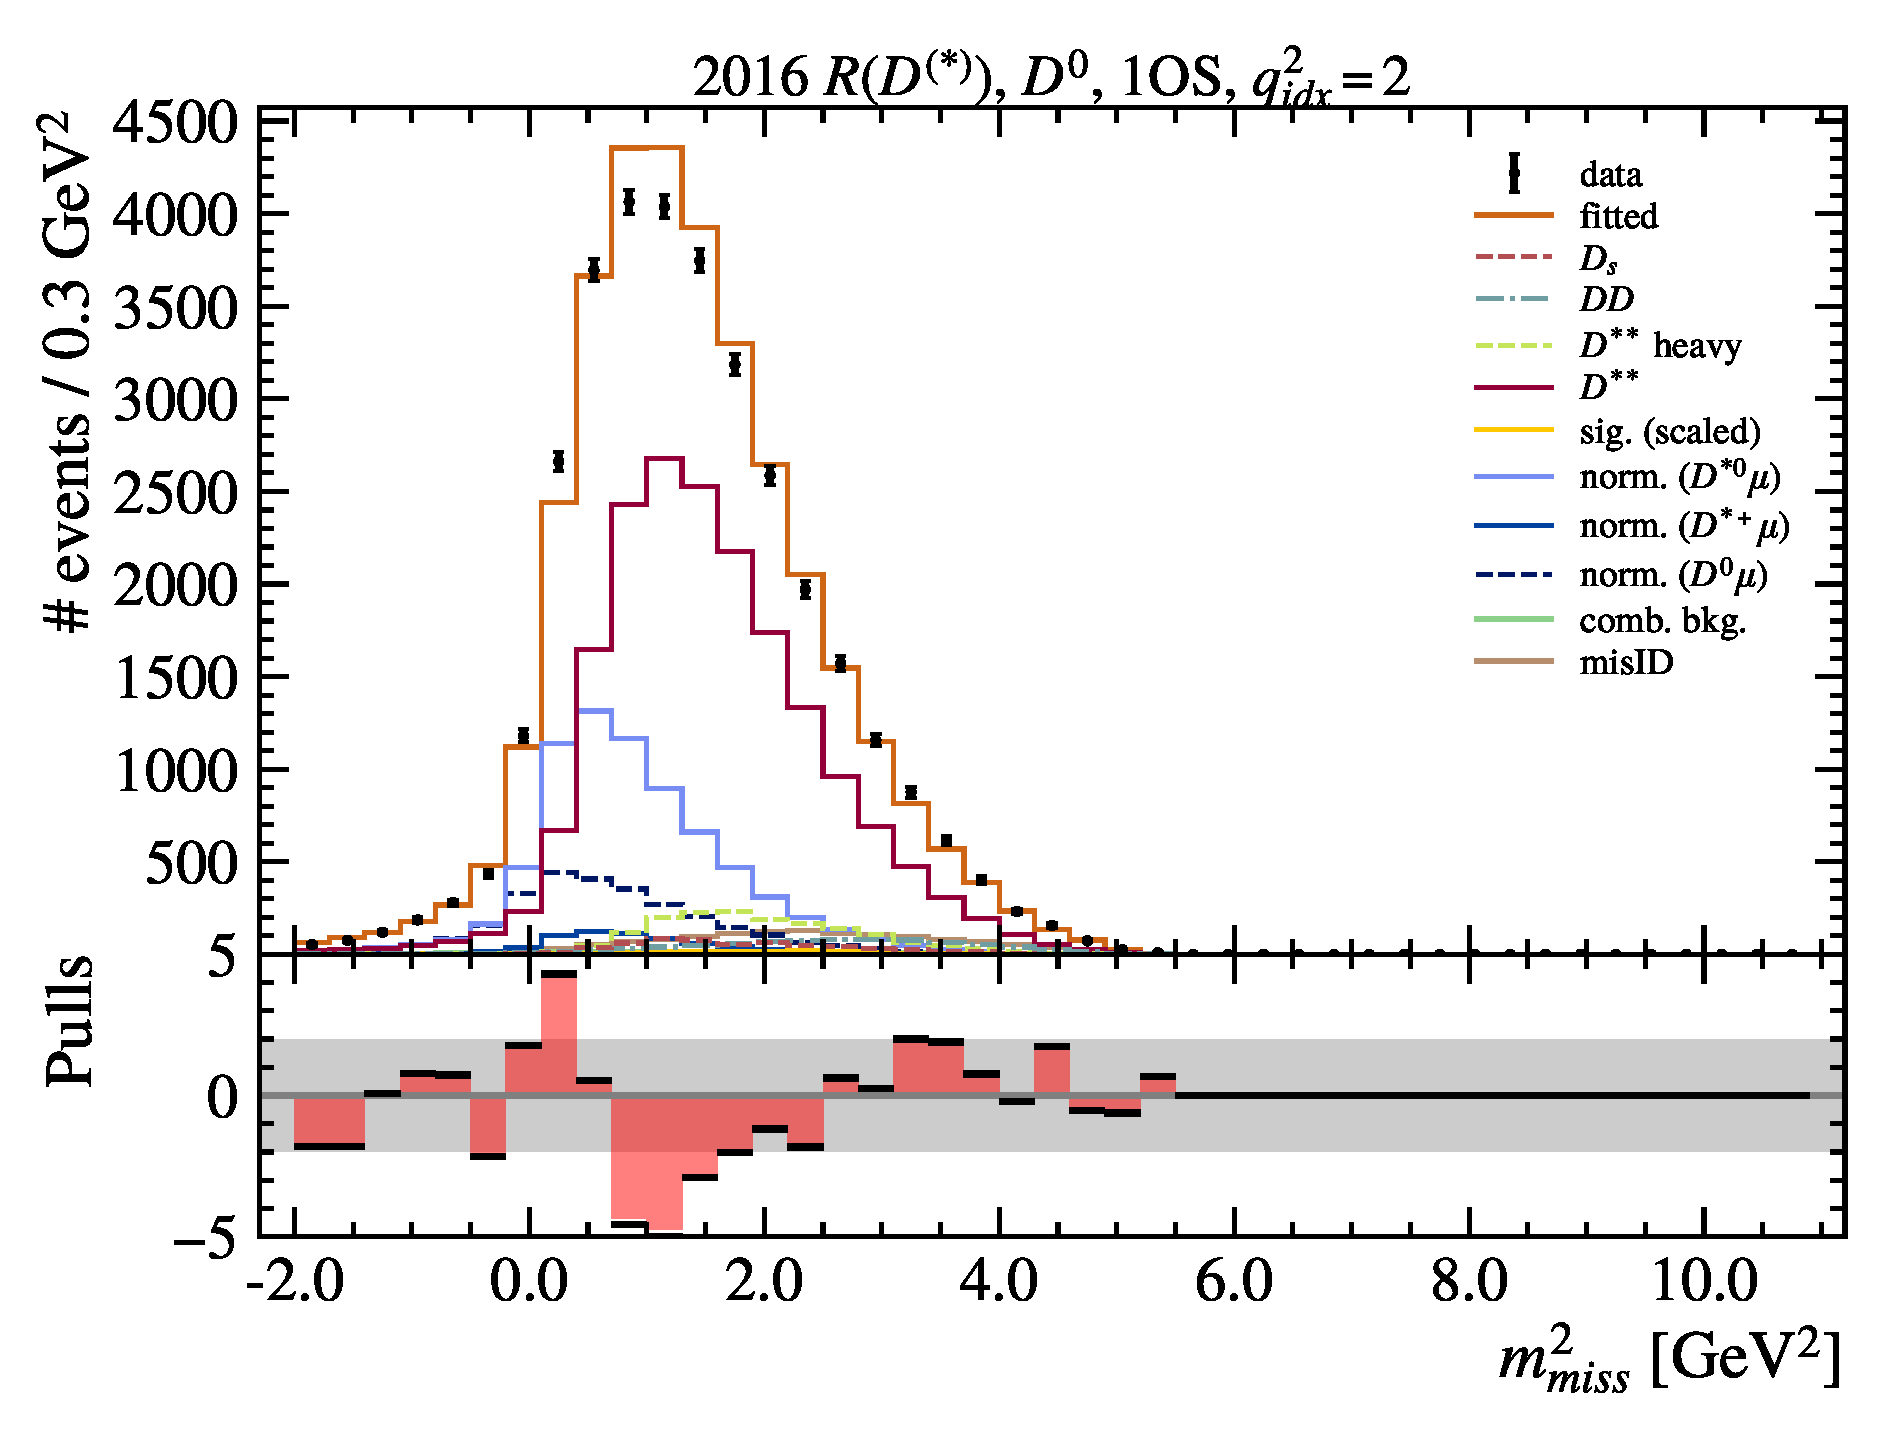
\includegraphics[width=0.24\textwidth]{./figs-fit-fit-results/ctrl-fit/lines_q2_slices/fit_result-lines_q2_idx2-D0-1os-mmiss2.pdf}
    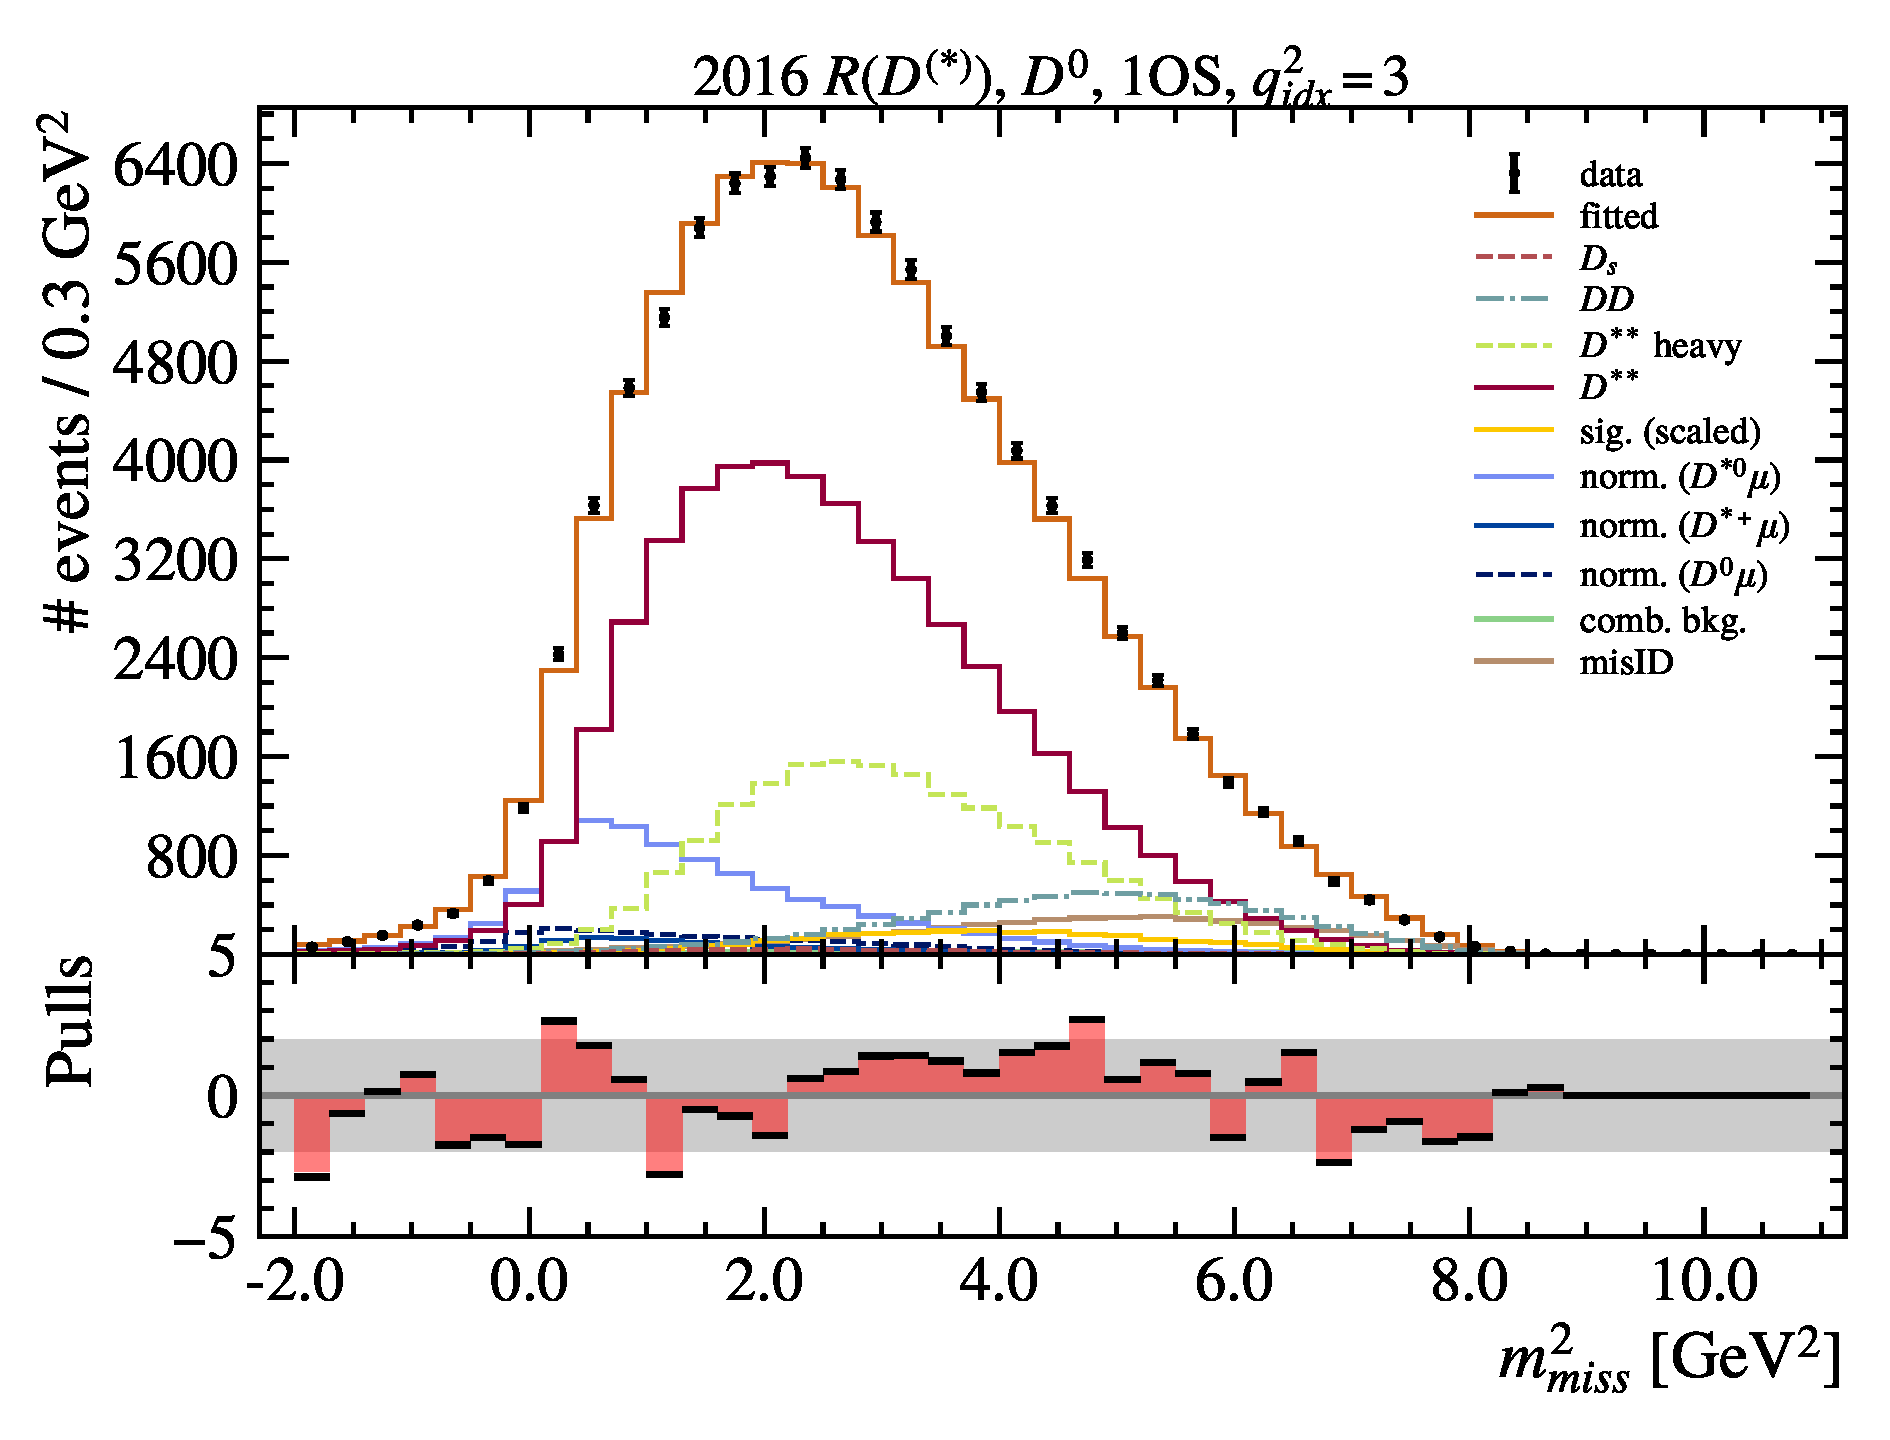
\includegraphics[width=0.24\textwidth]{./figs-fit-fit-results/ctrl-fit/lines_q2_slices/fit_result-lines_q2_idx3-D0-1os-mmiss2.pdf}
    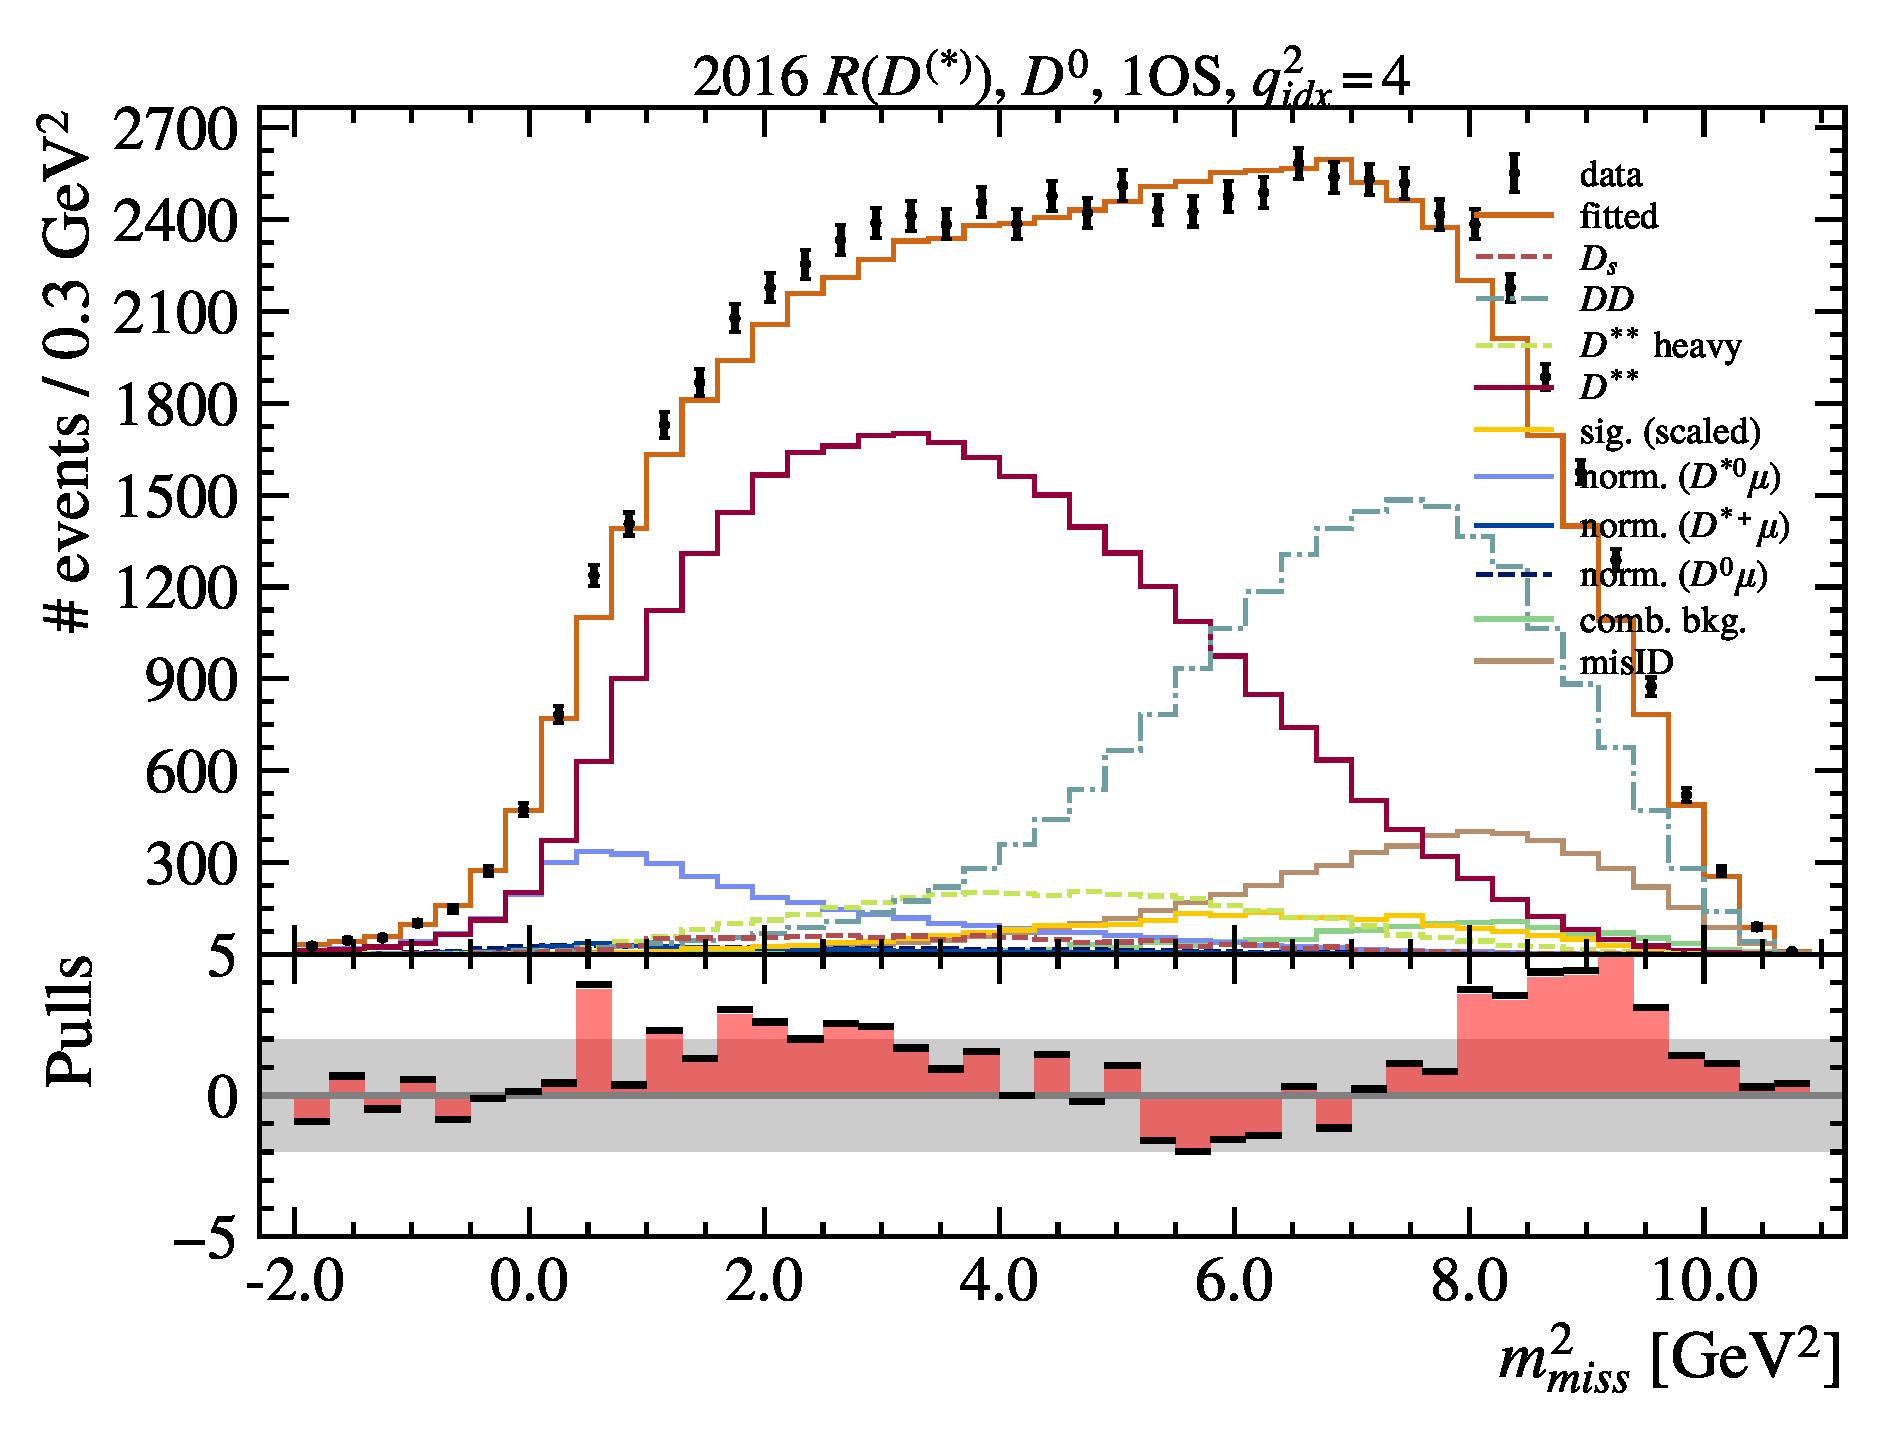
\includegraphics[width=0.24\textwidth]{./figs-fit-fit-results/ctrl-fit/lines_q2_slices/fit_result-lines_q2_idx4-D0-1os-mmiss2.pdf}

    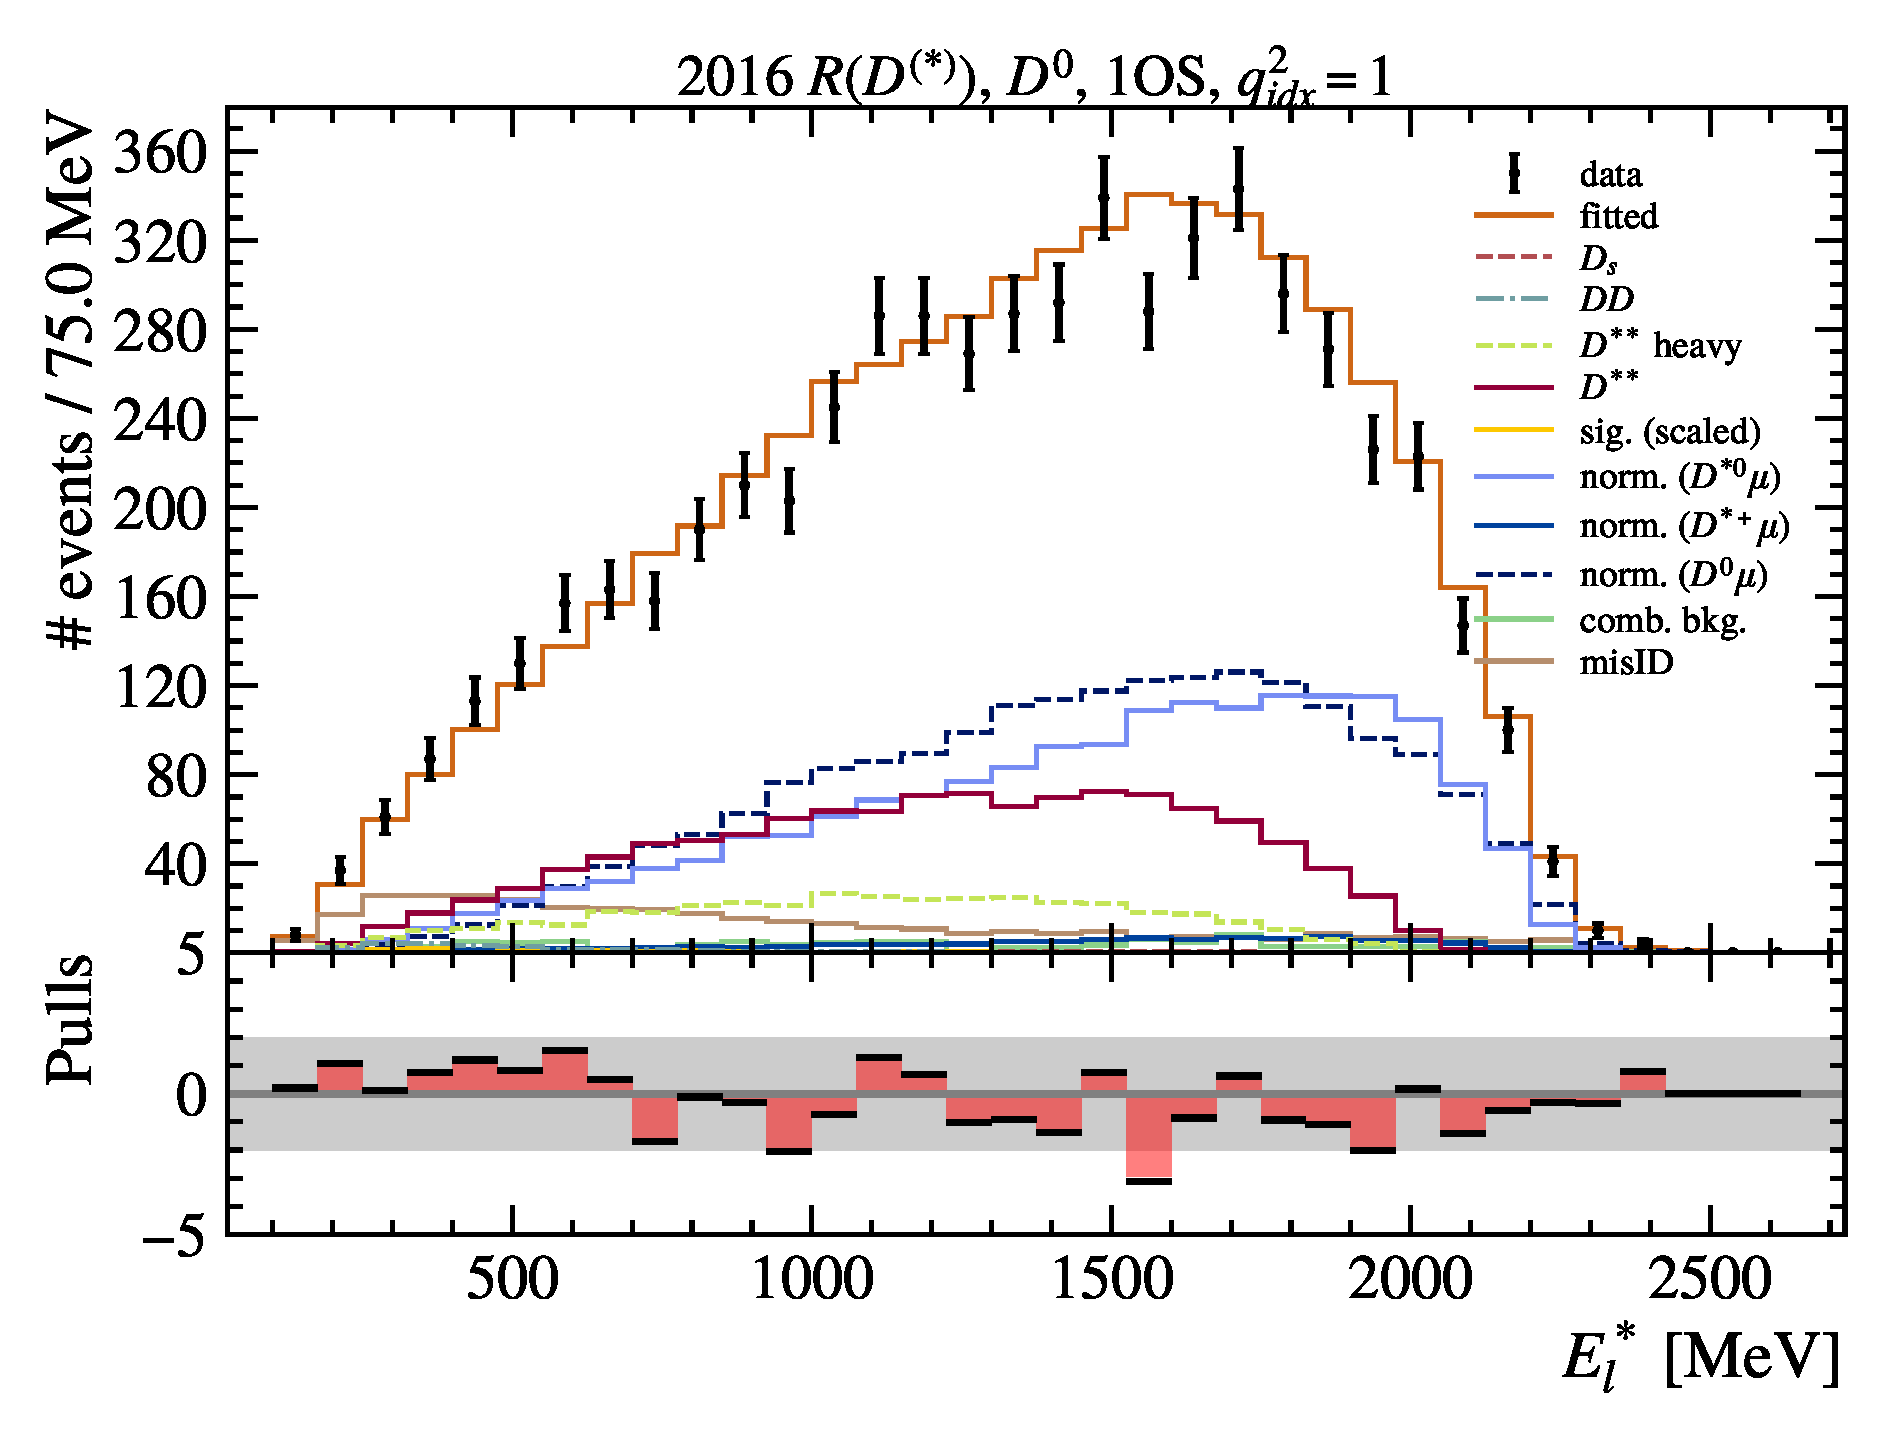
\includegraphics[width=0.24\textwidth]{./figs-fit-fit-results/ctrl-fit/lines_q2_slices/fit_result-lines_q2_idx1-D0-1os-el.pdf}
    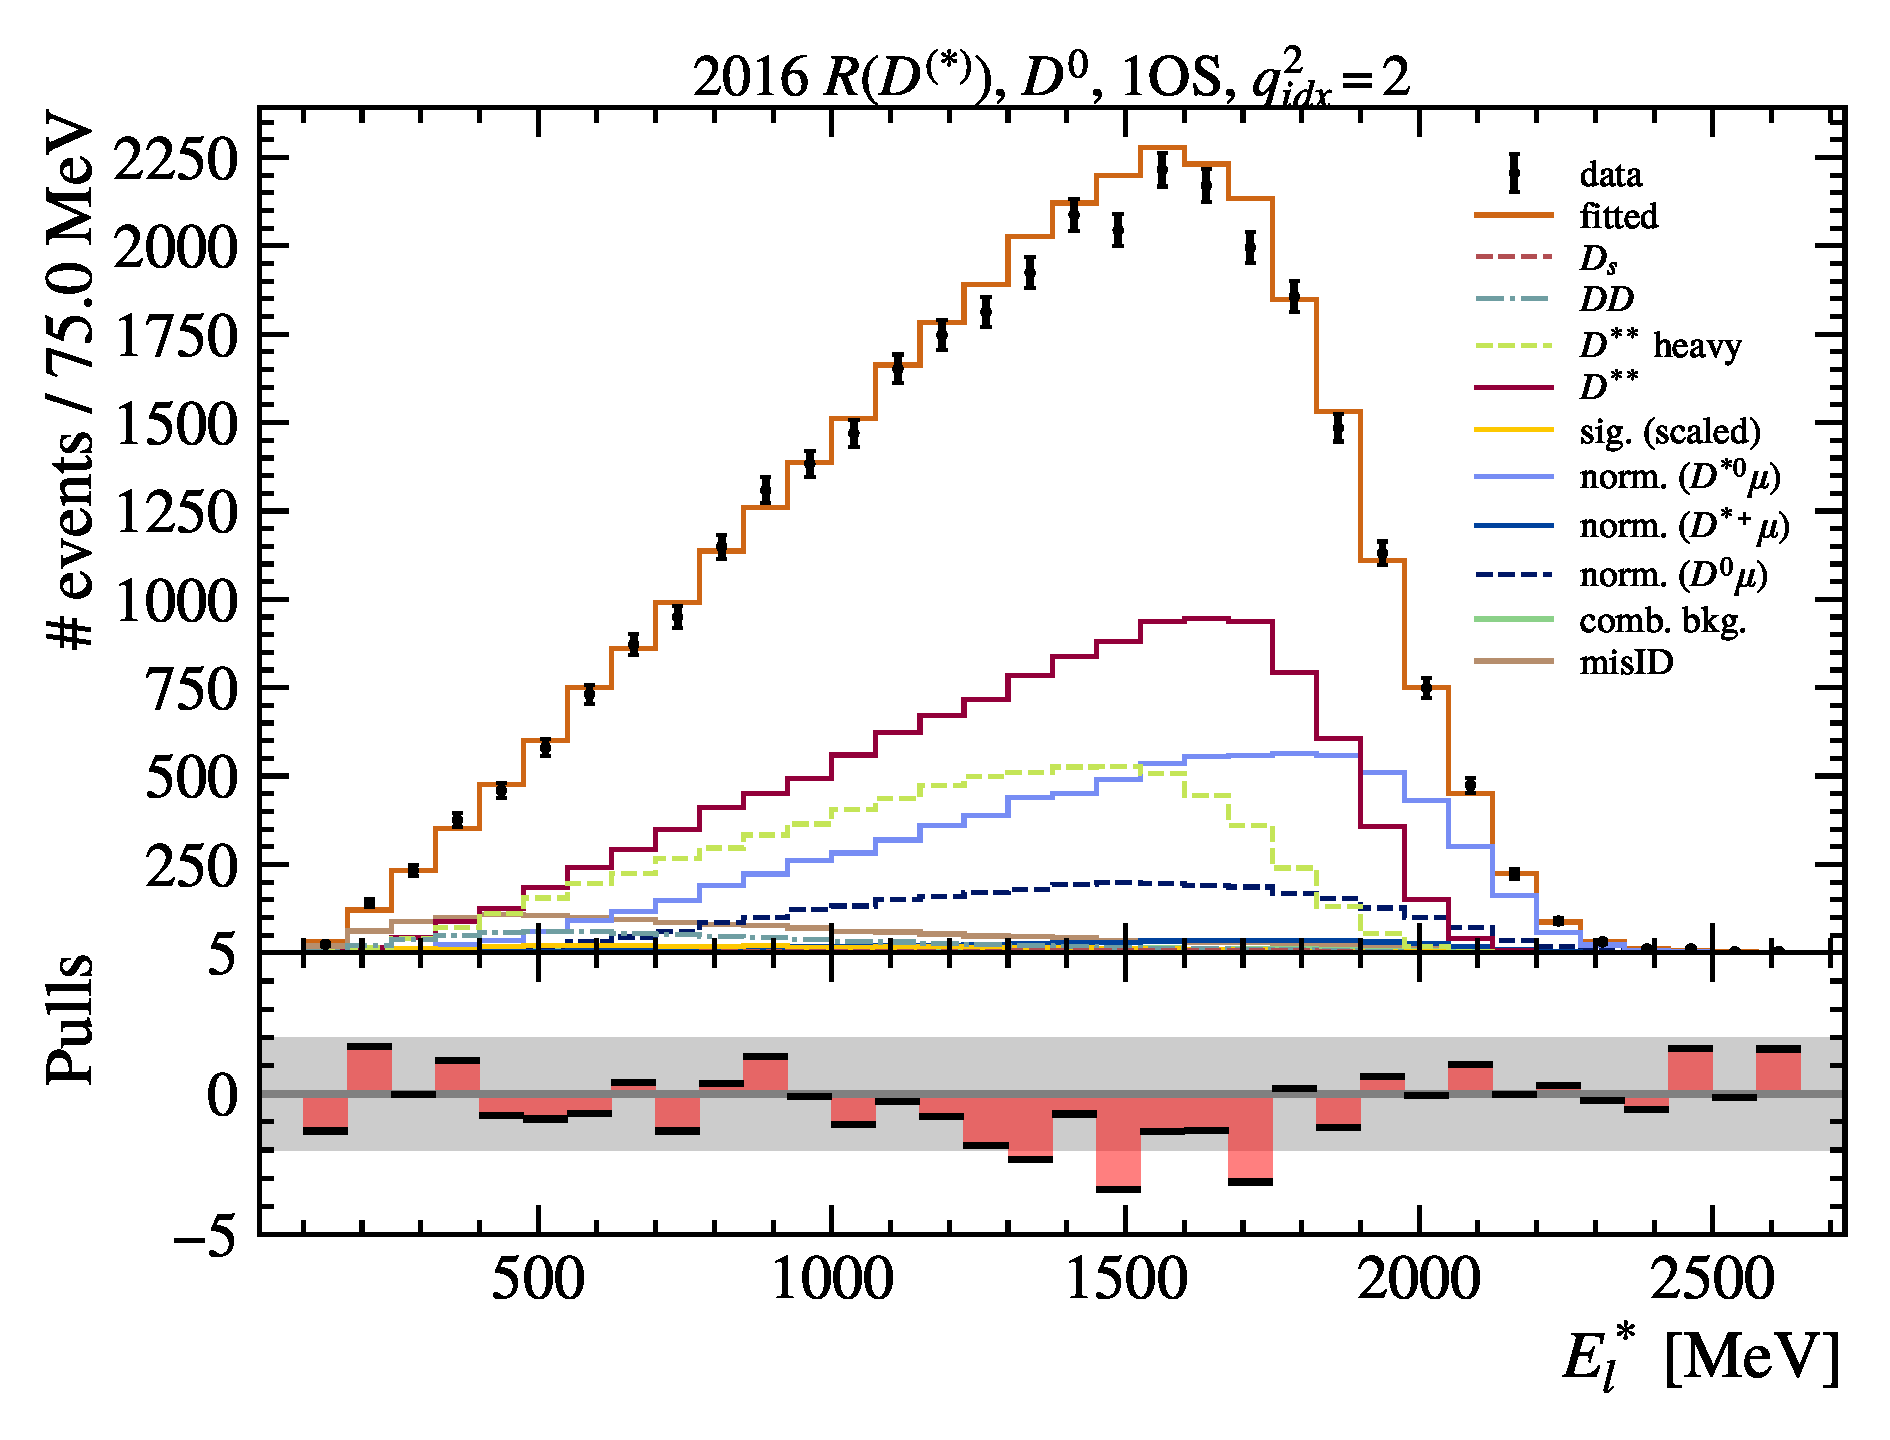
\includegraphics[width=0.24\textwidth]{./figs-fit-fit-results/ctrl-fit/lines_q2_slices/fit_result-lines_q2_idx2-D0-1os-el.pdf}
    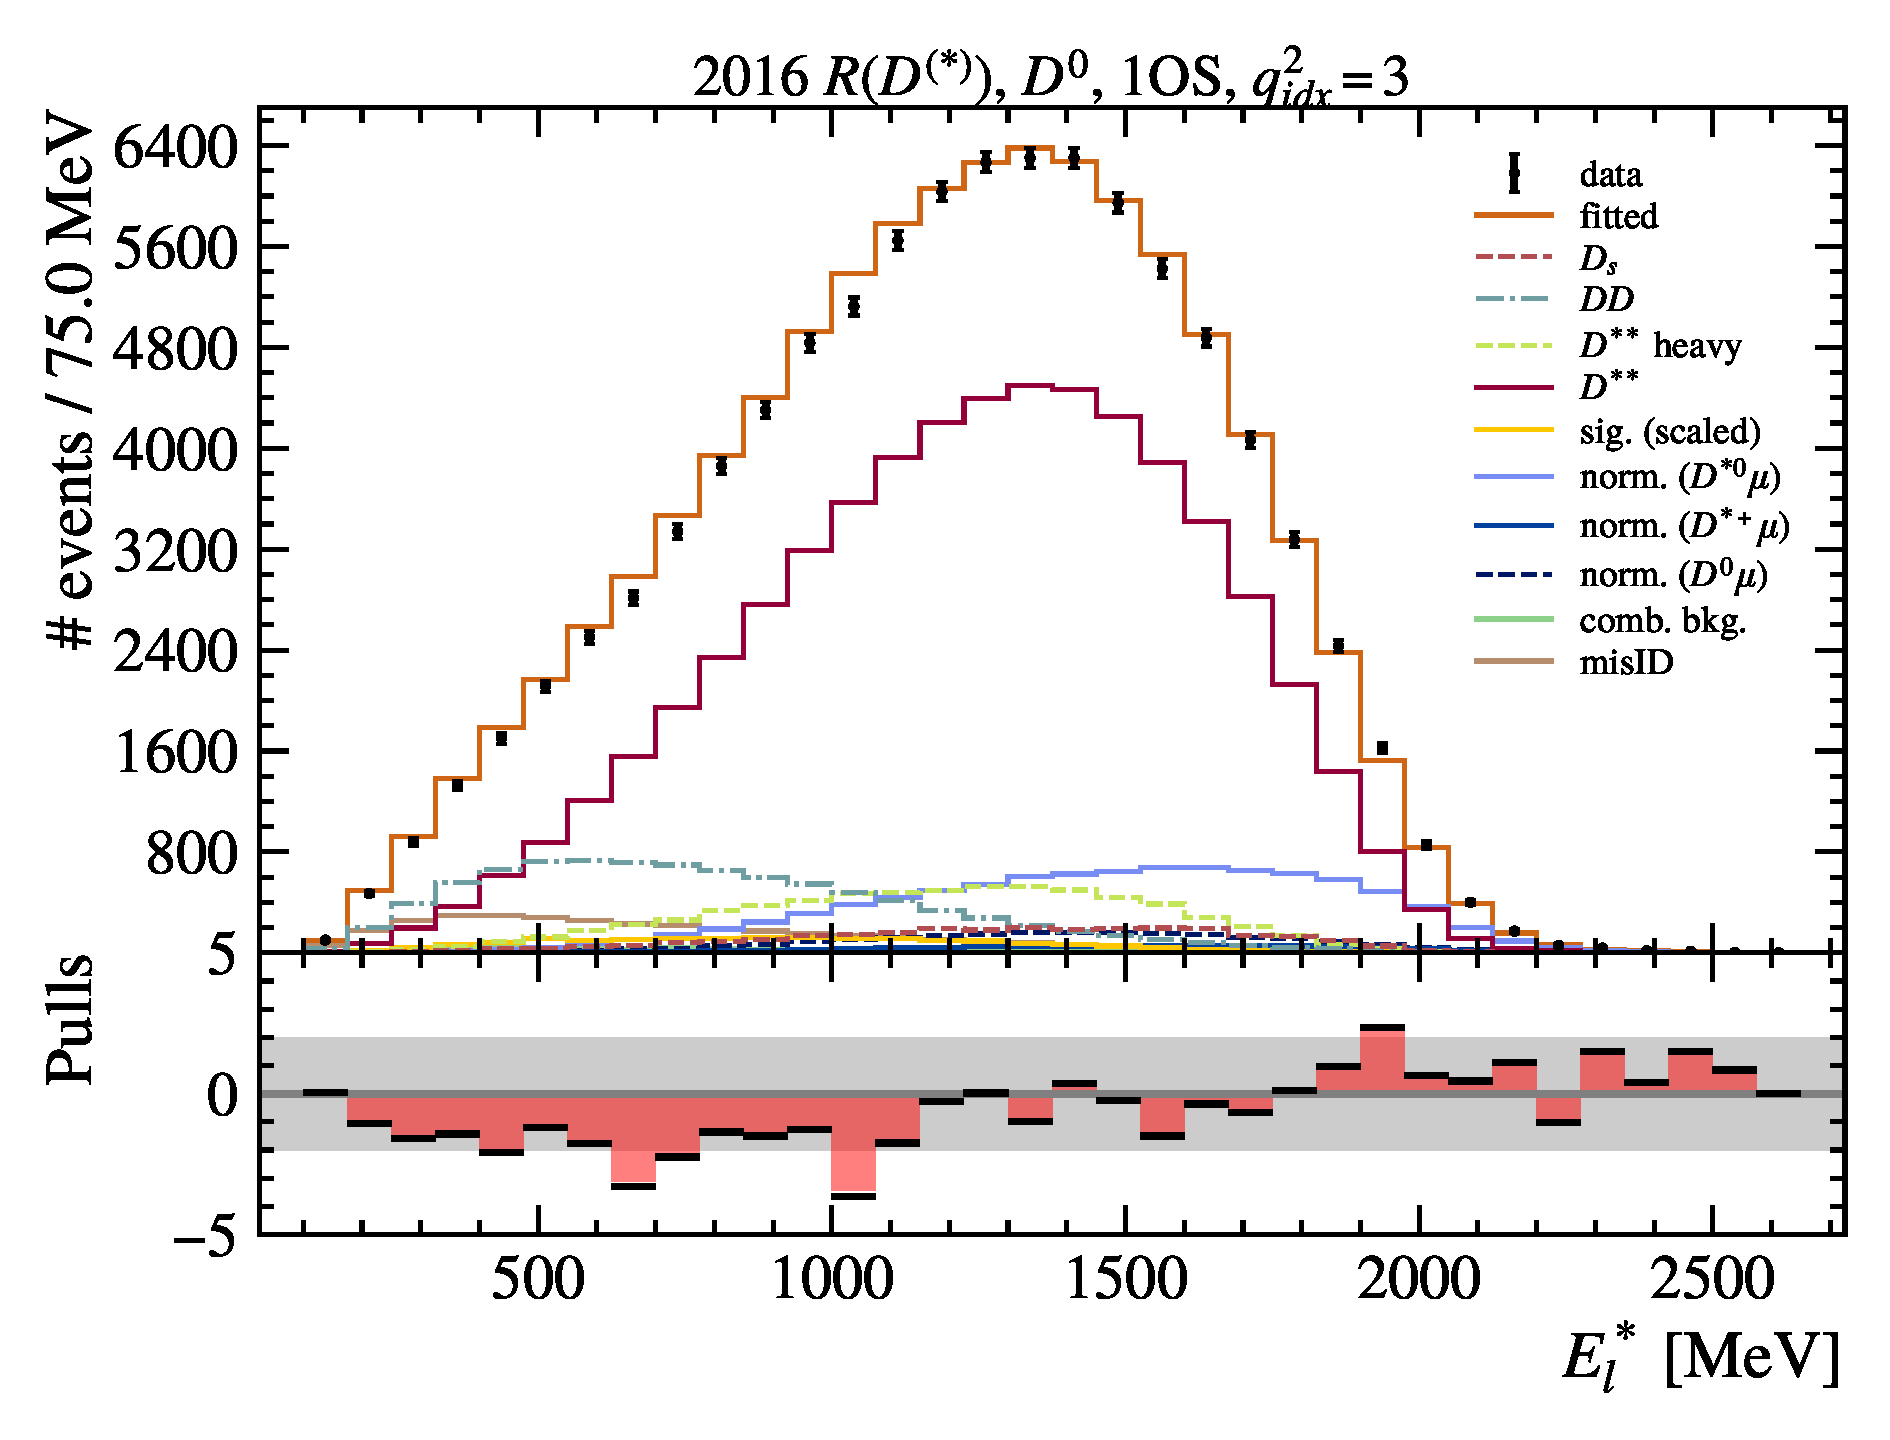
\includegraphics[width=0.24\textwidth]{./figs-fit-fit-results/ctrl-fit/lines_q2_slices/fit_result-lines_q2_idx3-D0-1os-el.pdf}
    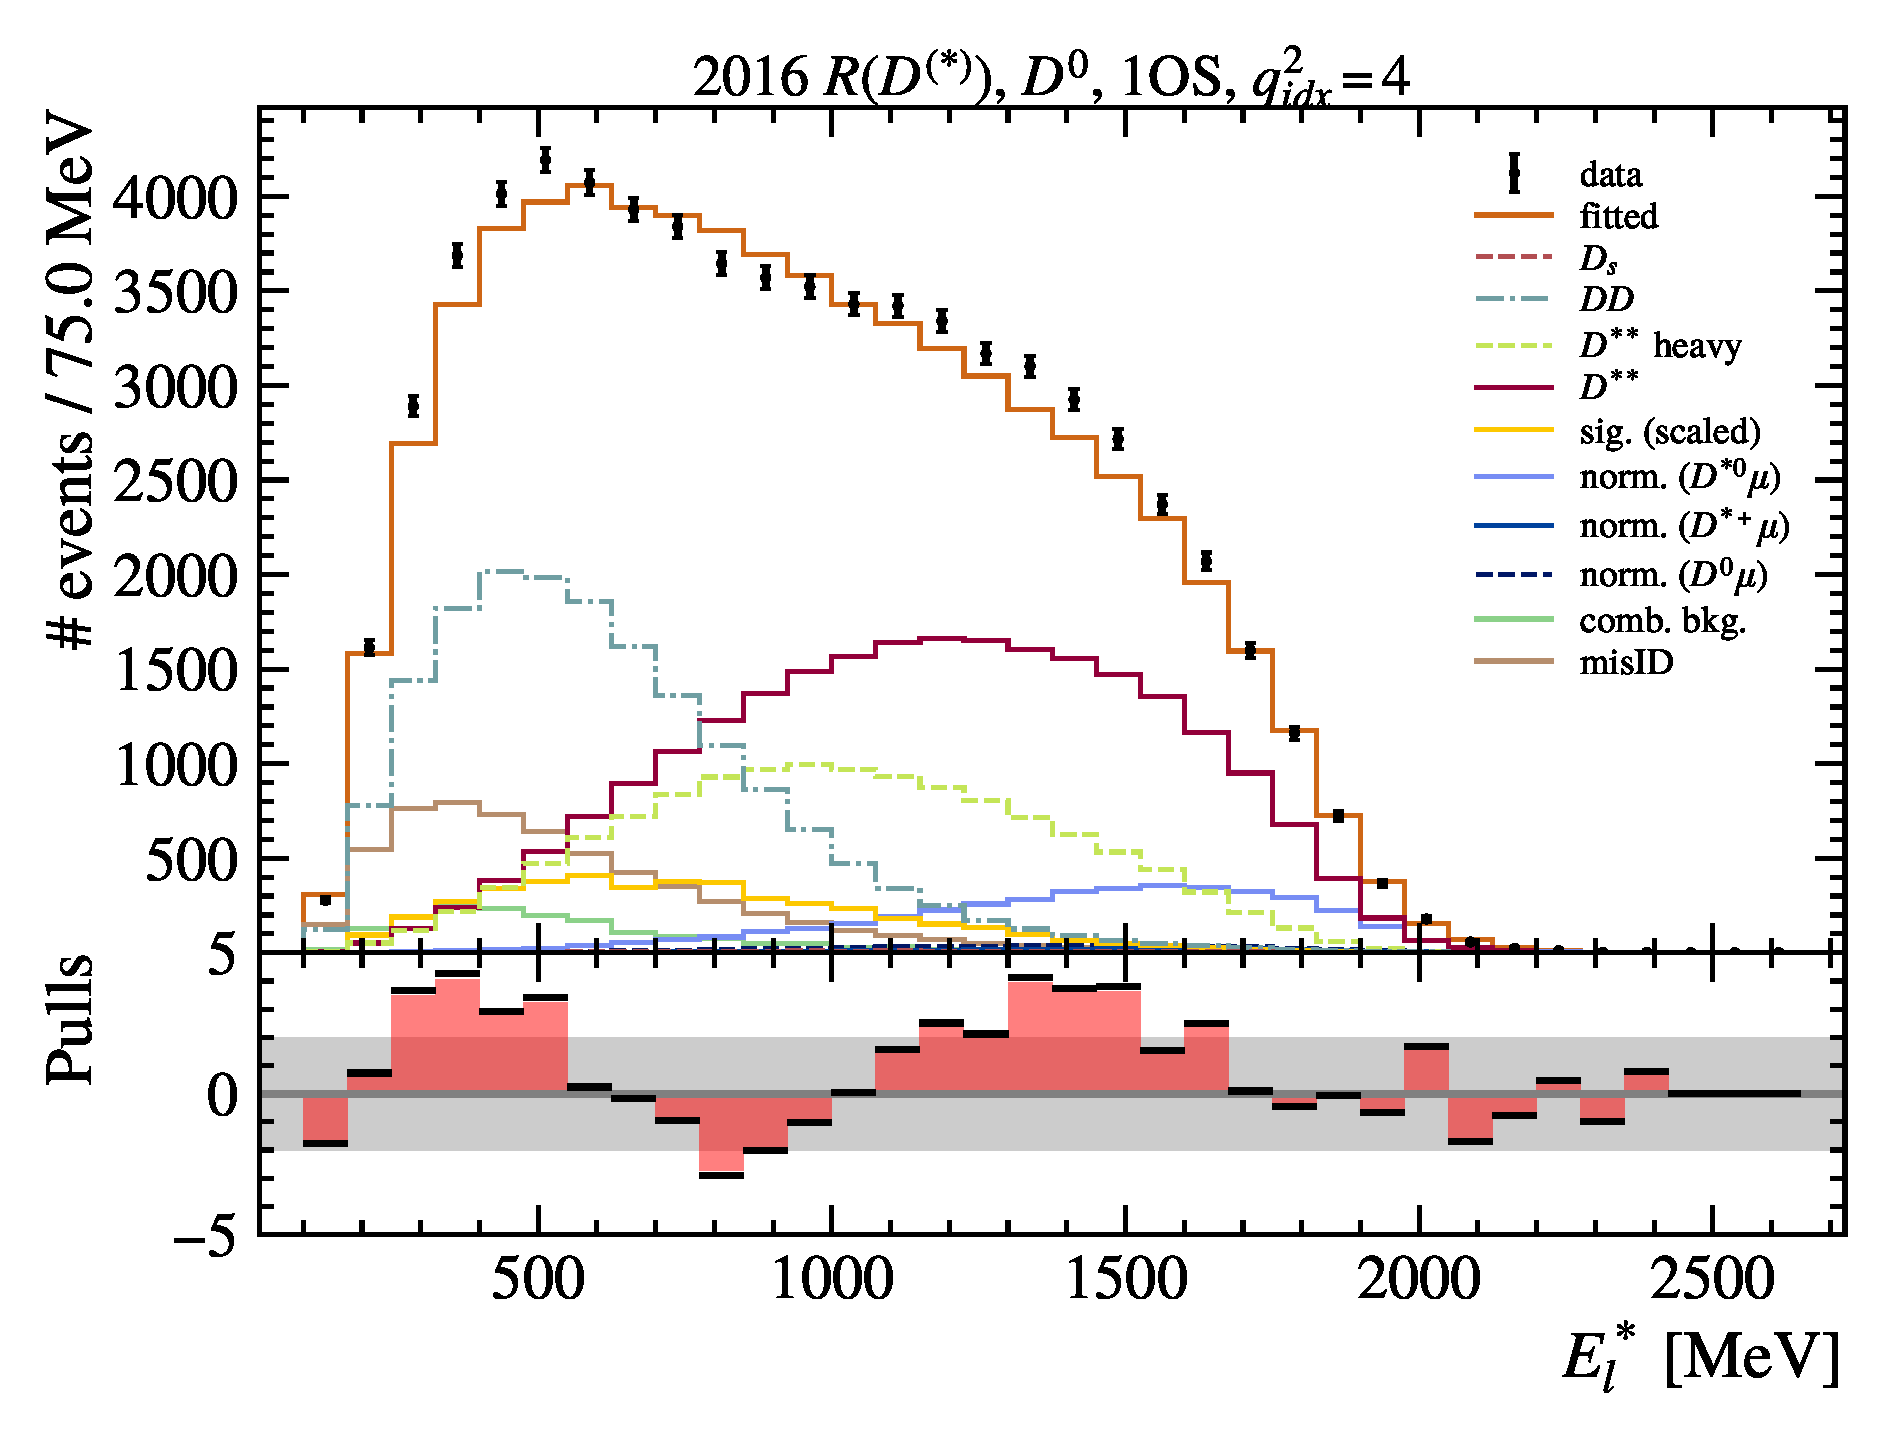
\includegraphics[width=0.24\textwidth]{./figs-fit-fit-results/ctrl-fit/lines_q2_slices/fit_result-lines_q2_idx4-D0-1os-el.pdf}

    \caption{Control fit for 1OS sample, \Dz channel.}
    \label{fig:ctrl-1os-d0}
\end{figure}

\begin{figure}[!htb]
    \centering
    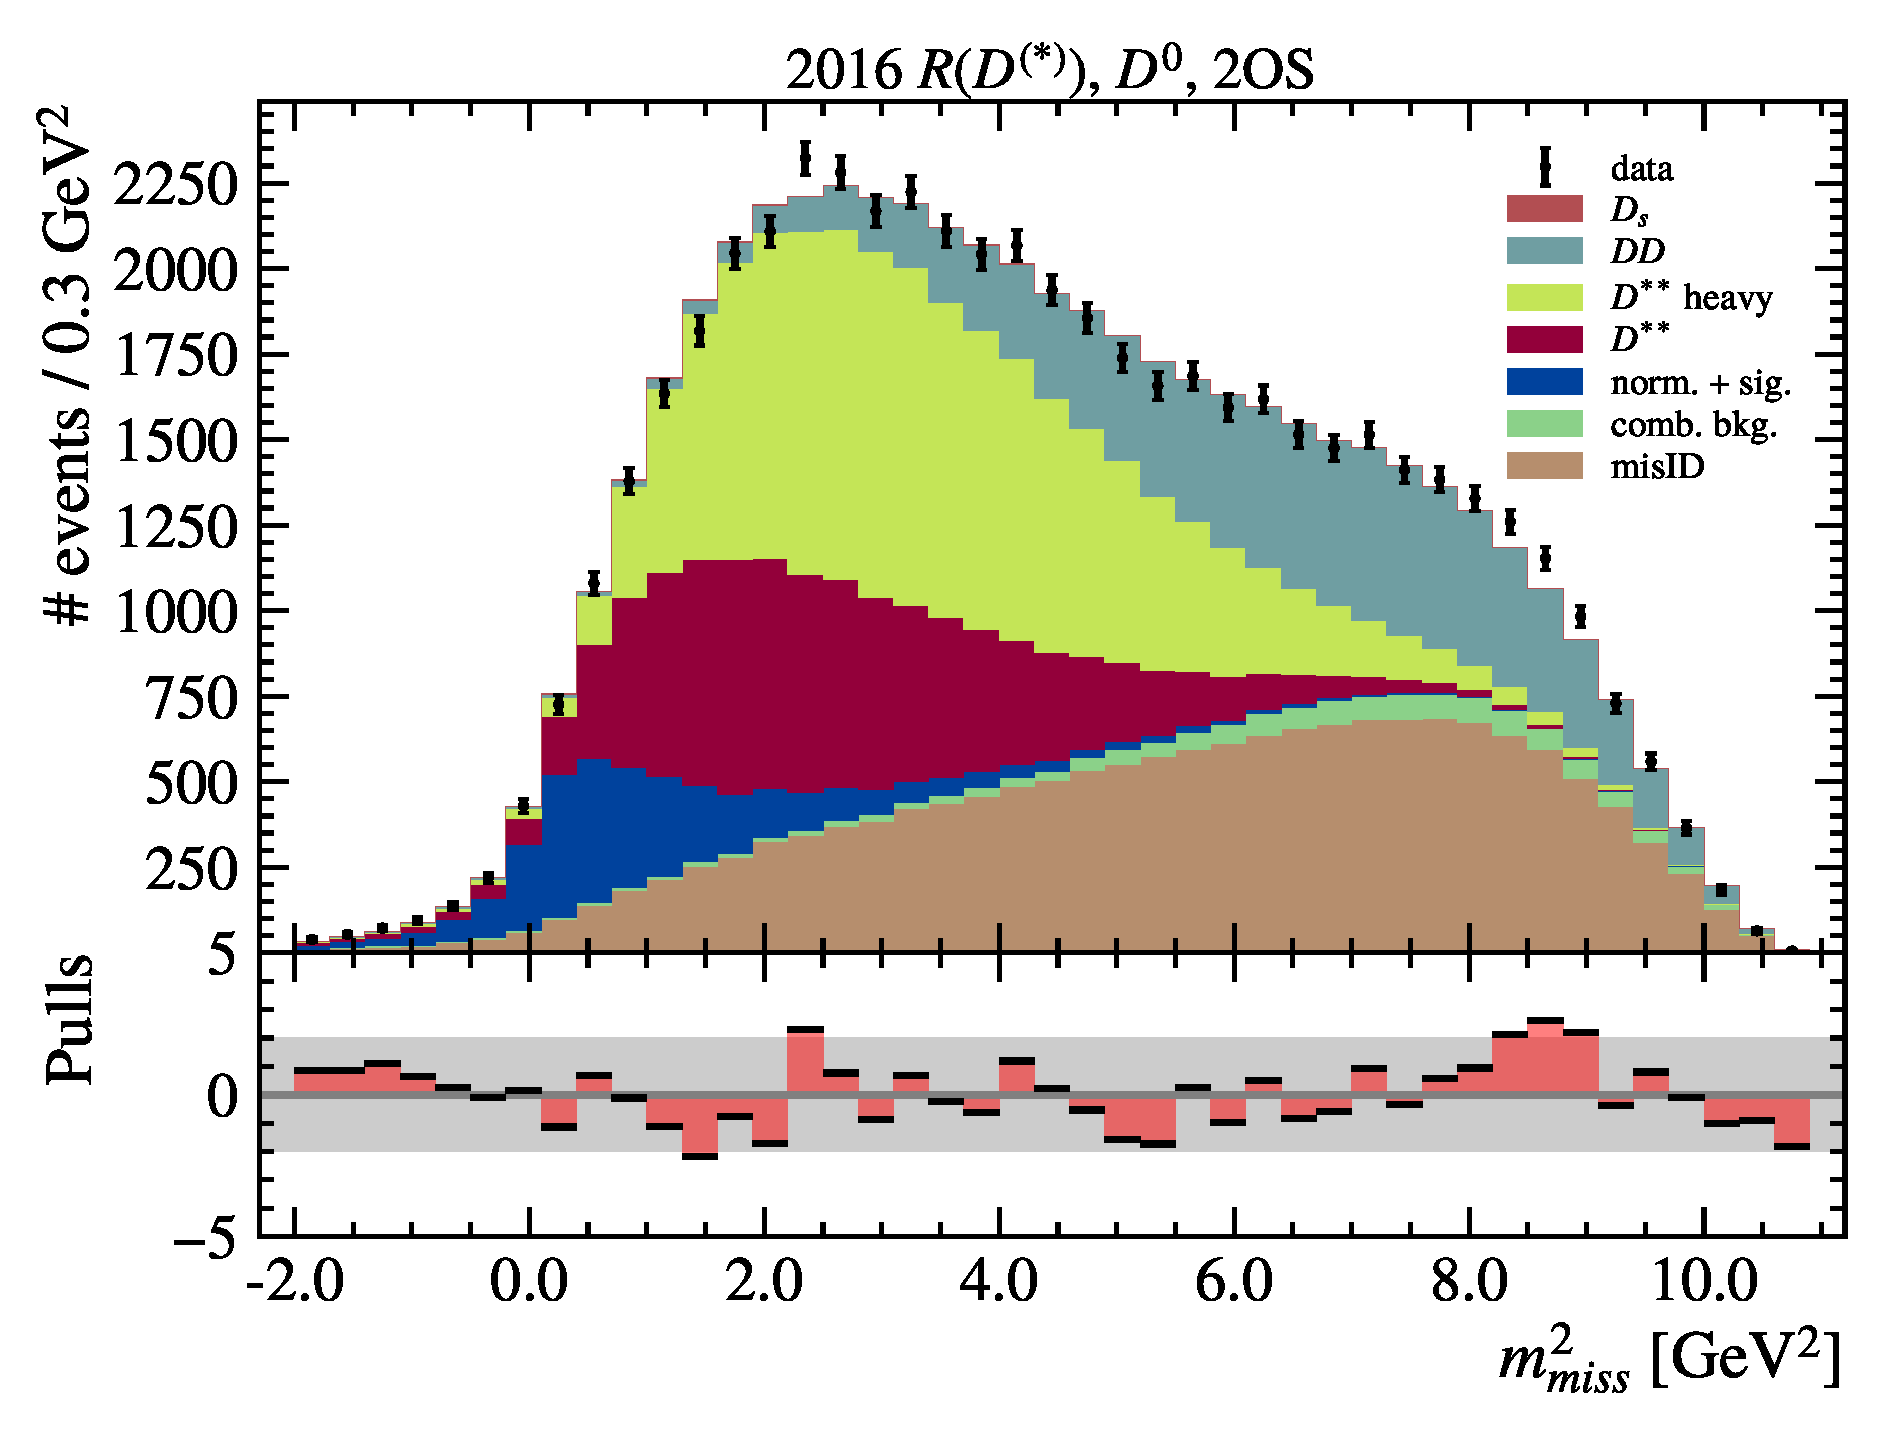
\includegraphics[width=0.32\textwidth]{./figs-fit-fit-results/ctrl-fit/stacked/fit_result-stacked-D0-2os-mmiss2.pdf}
    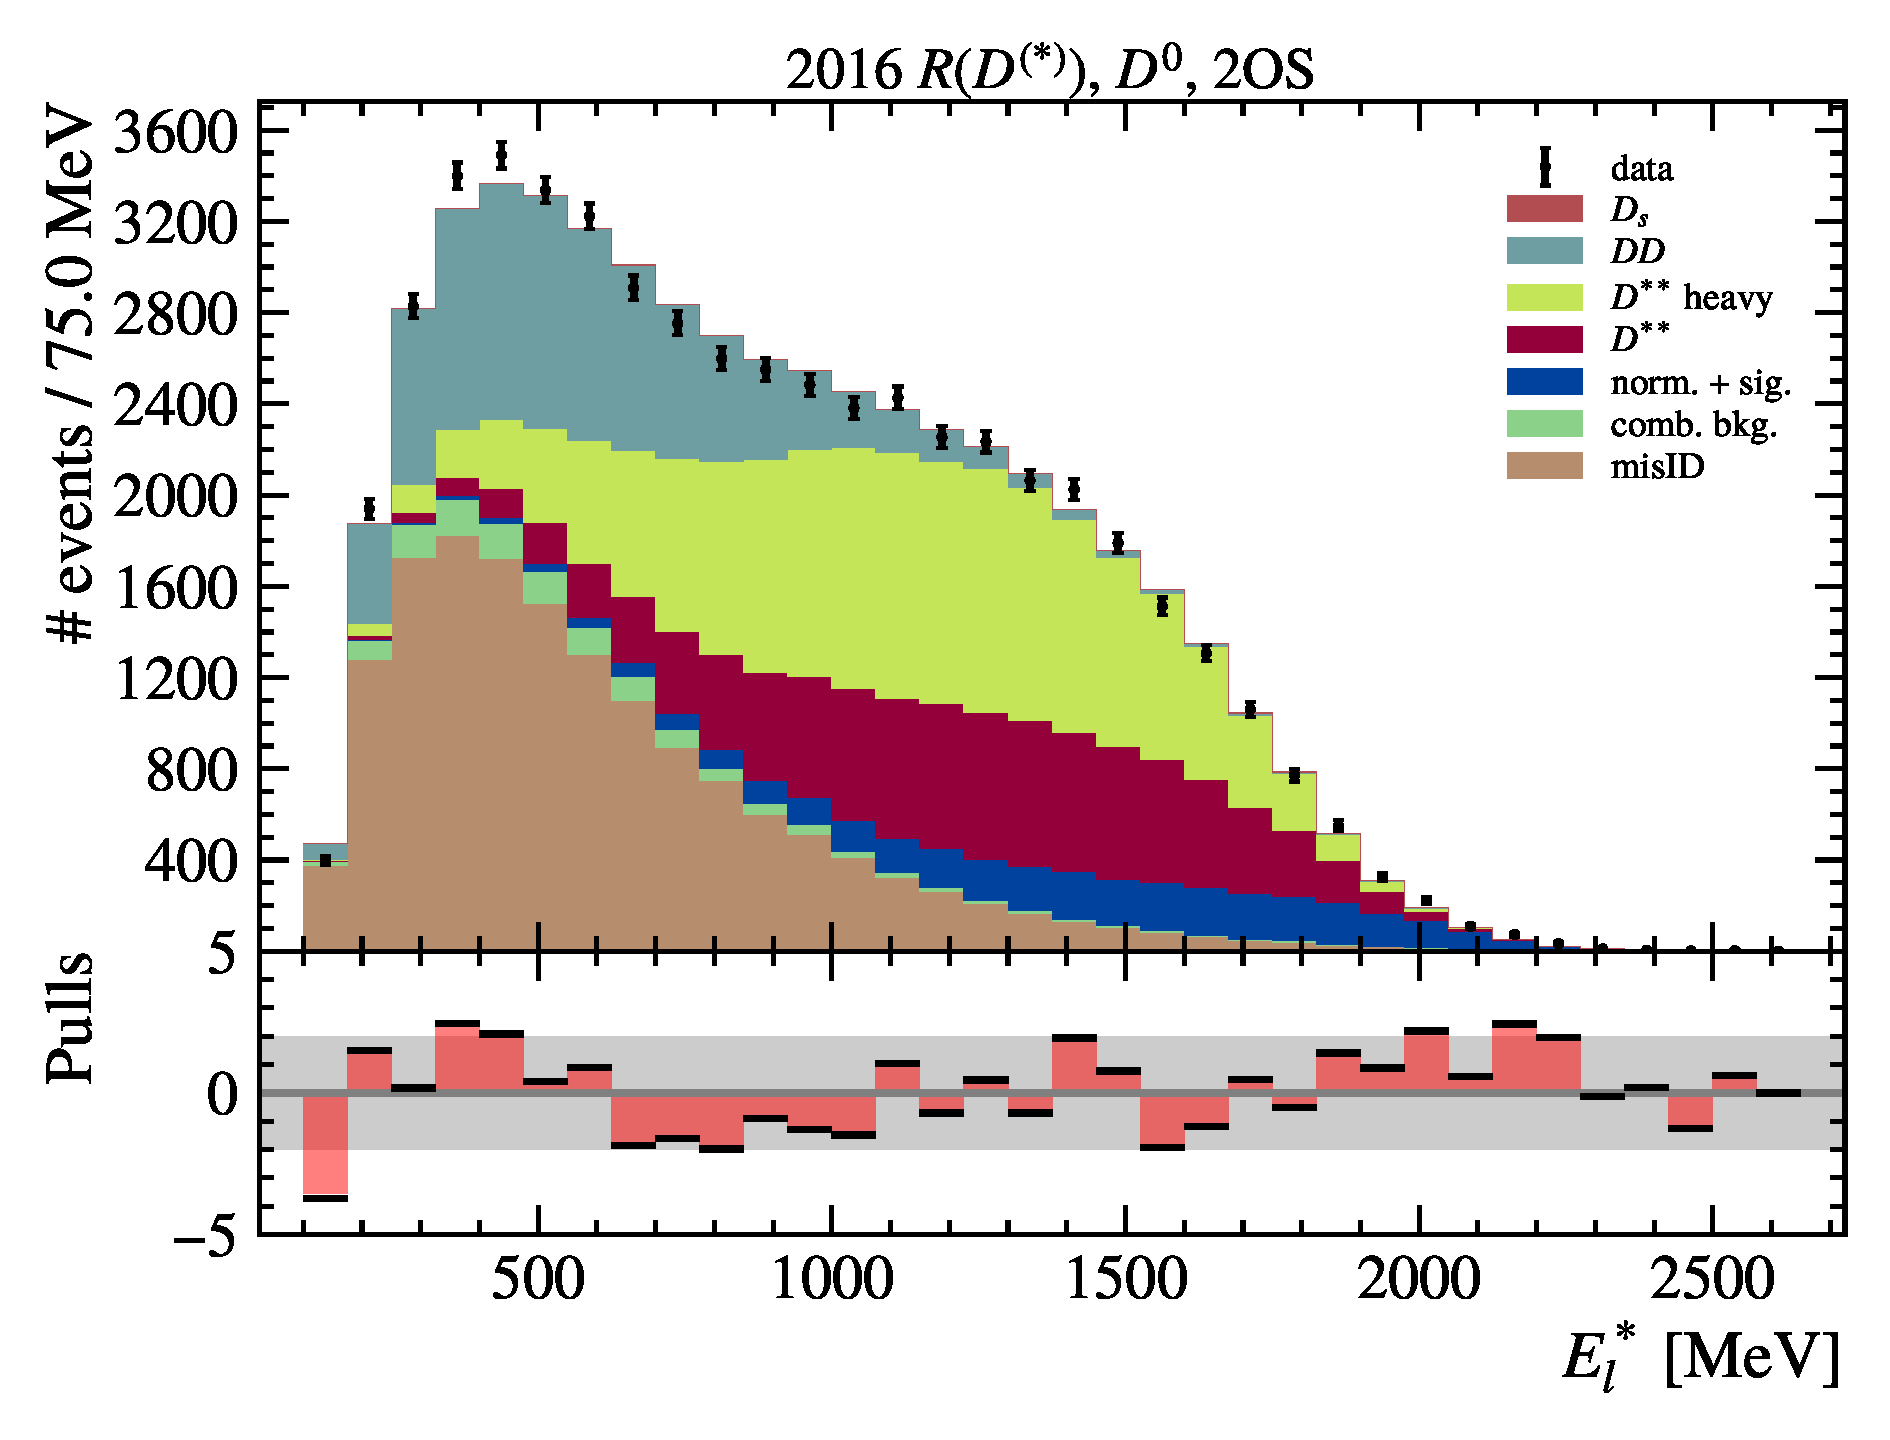
\includegraphics[width=0.32\textwidth]{./figs-fit-fit-results/ctrl-fit/stacked/fit_result-stacked-D0-2os-el.pdf}
    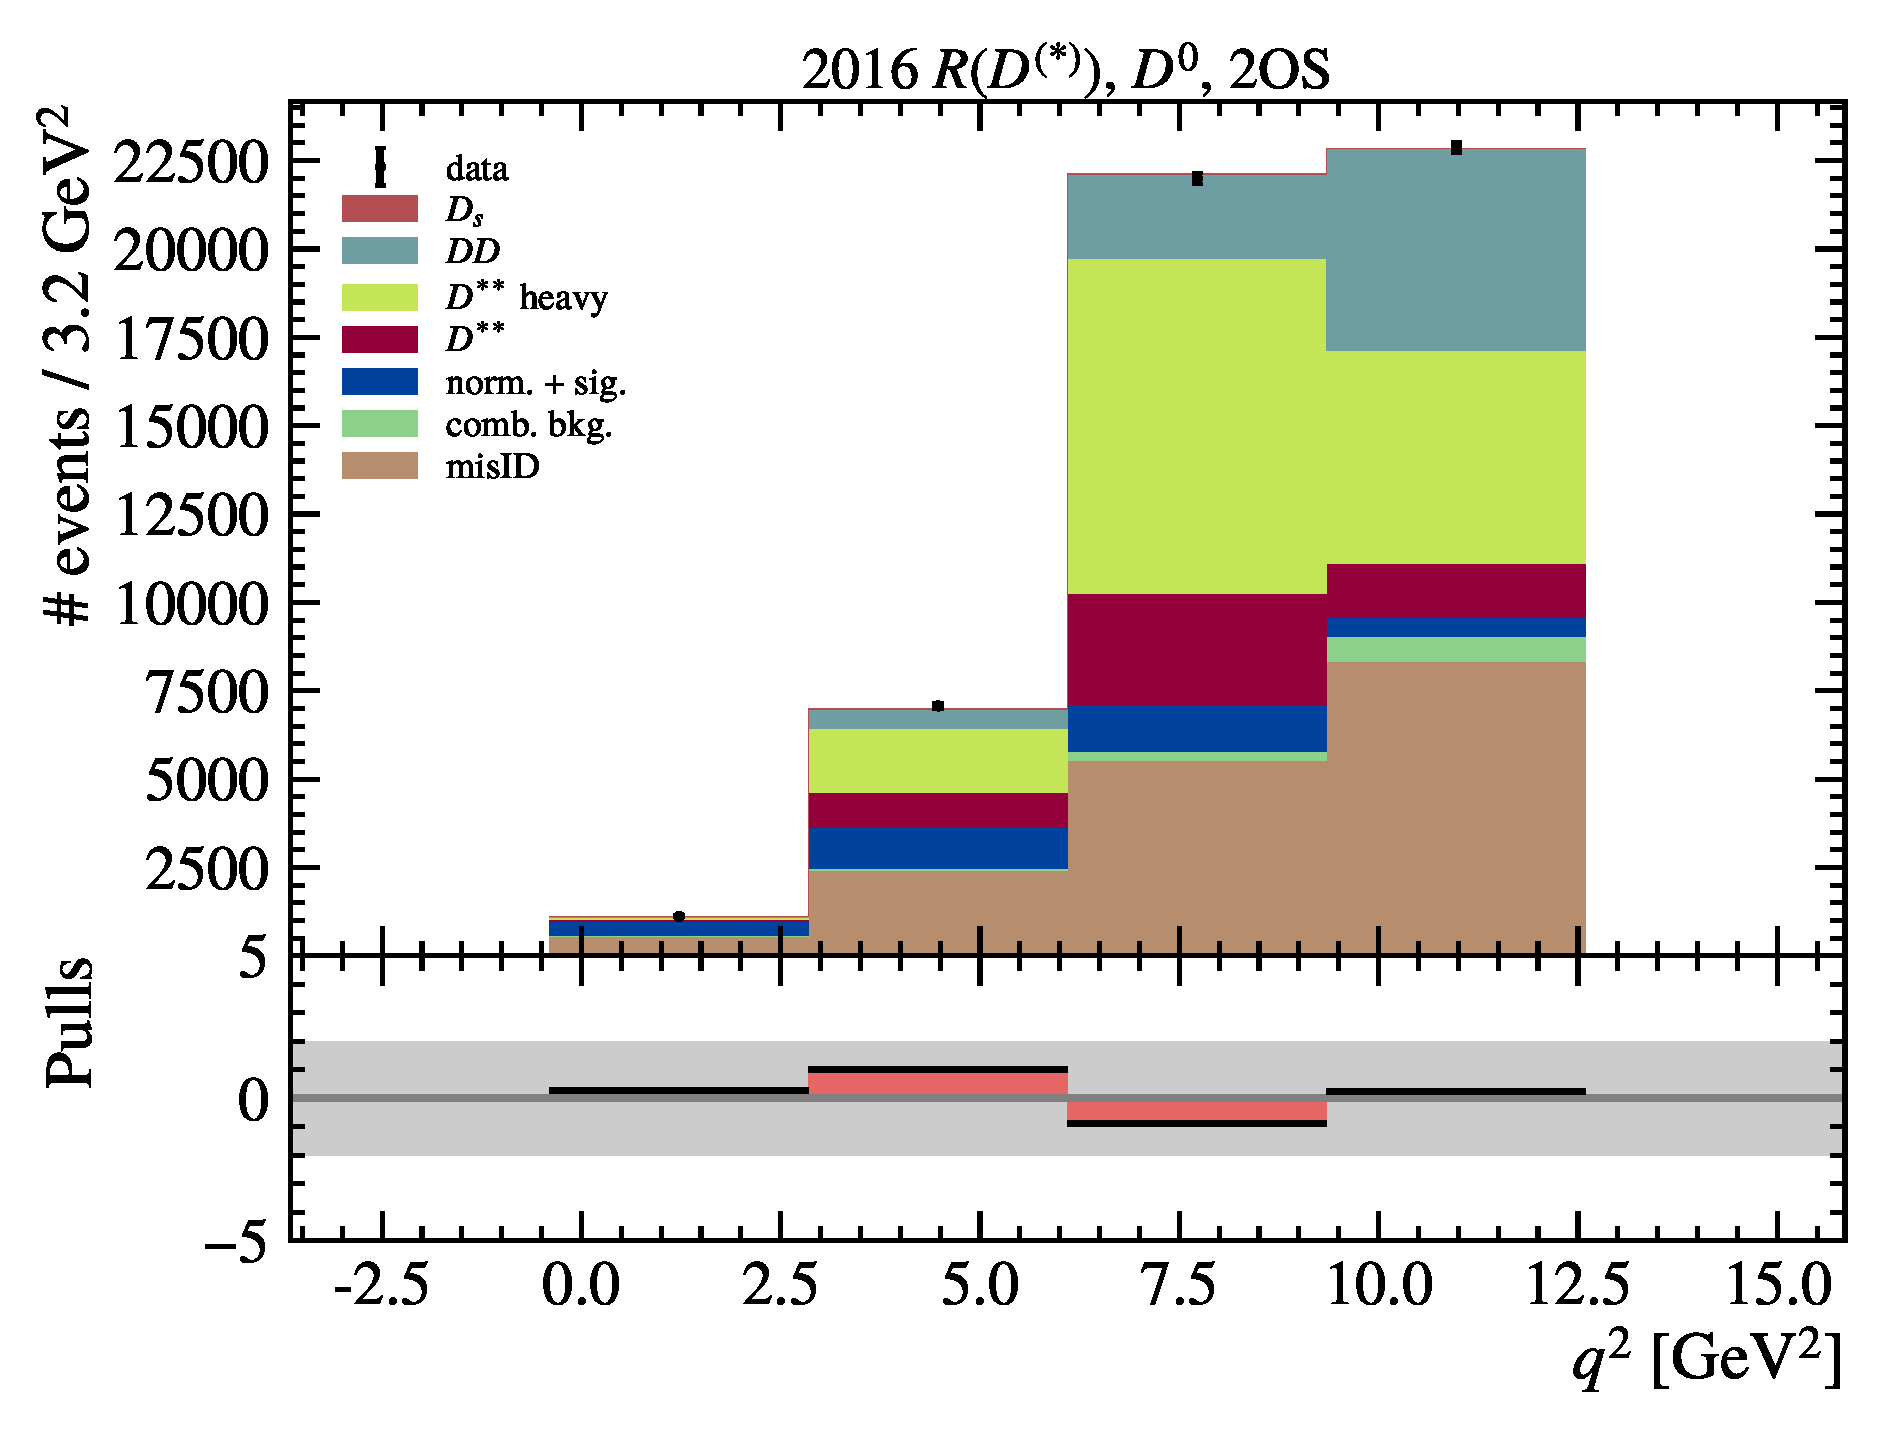
\includegraphics[width=0.32\textwidth]{./figs-fit-fit-results/ctrl-fit/stacked/fit_result-stacked-D0-2os-q2.pdf}

    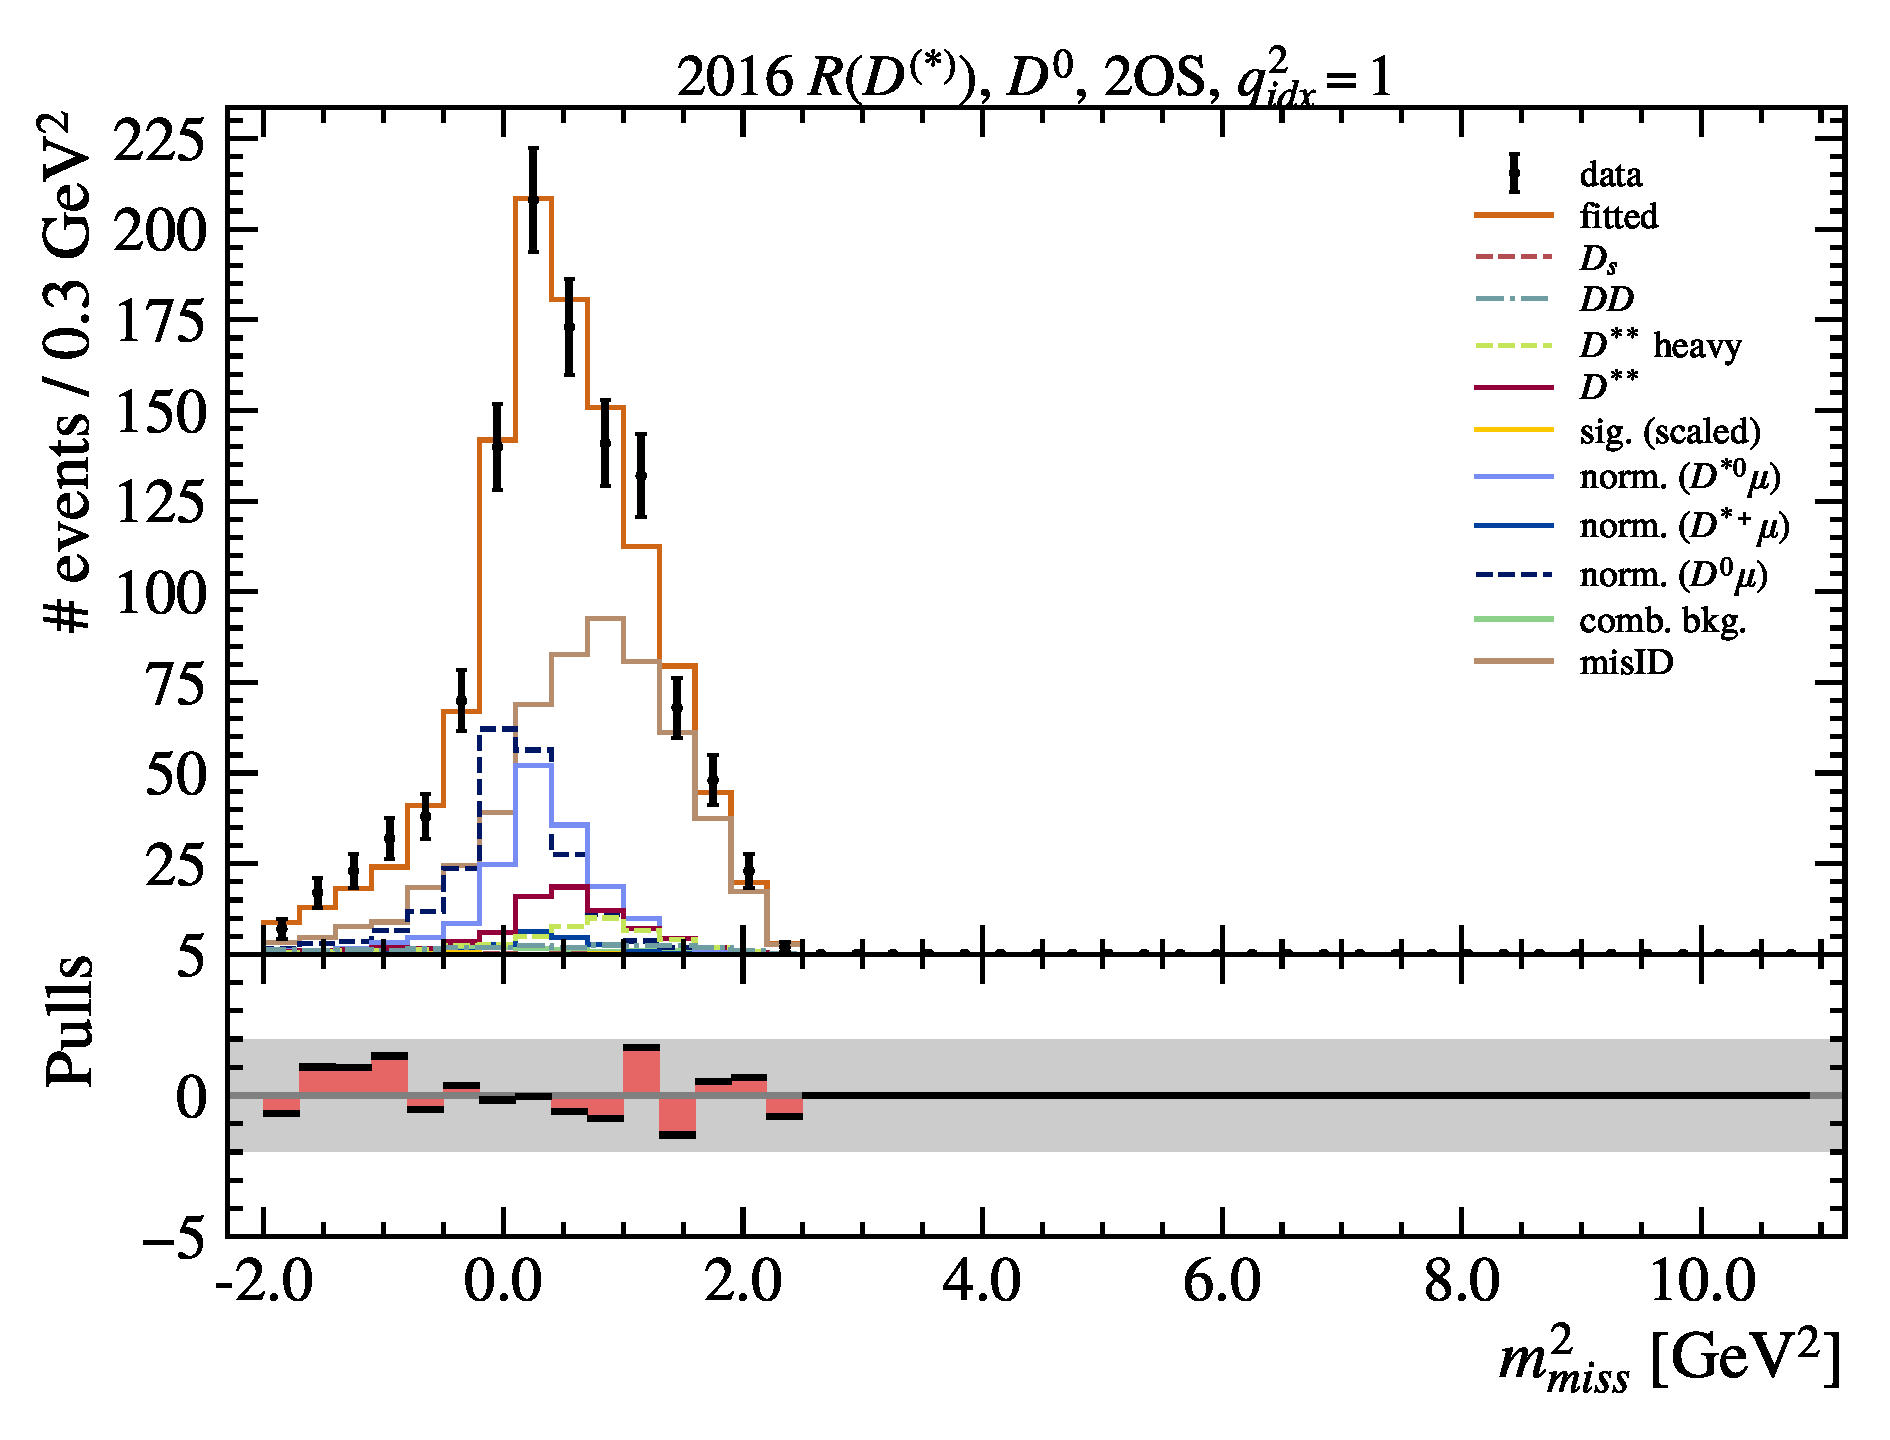
\includegraphics[width=0.24\textwidth]{./figs-fit-fit-results/ctrl-fit/lines_q2_slices/fit_result-lines_q2_idx1-D0-2os-mmiss2.pdf}
    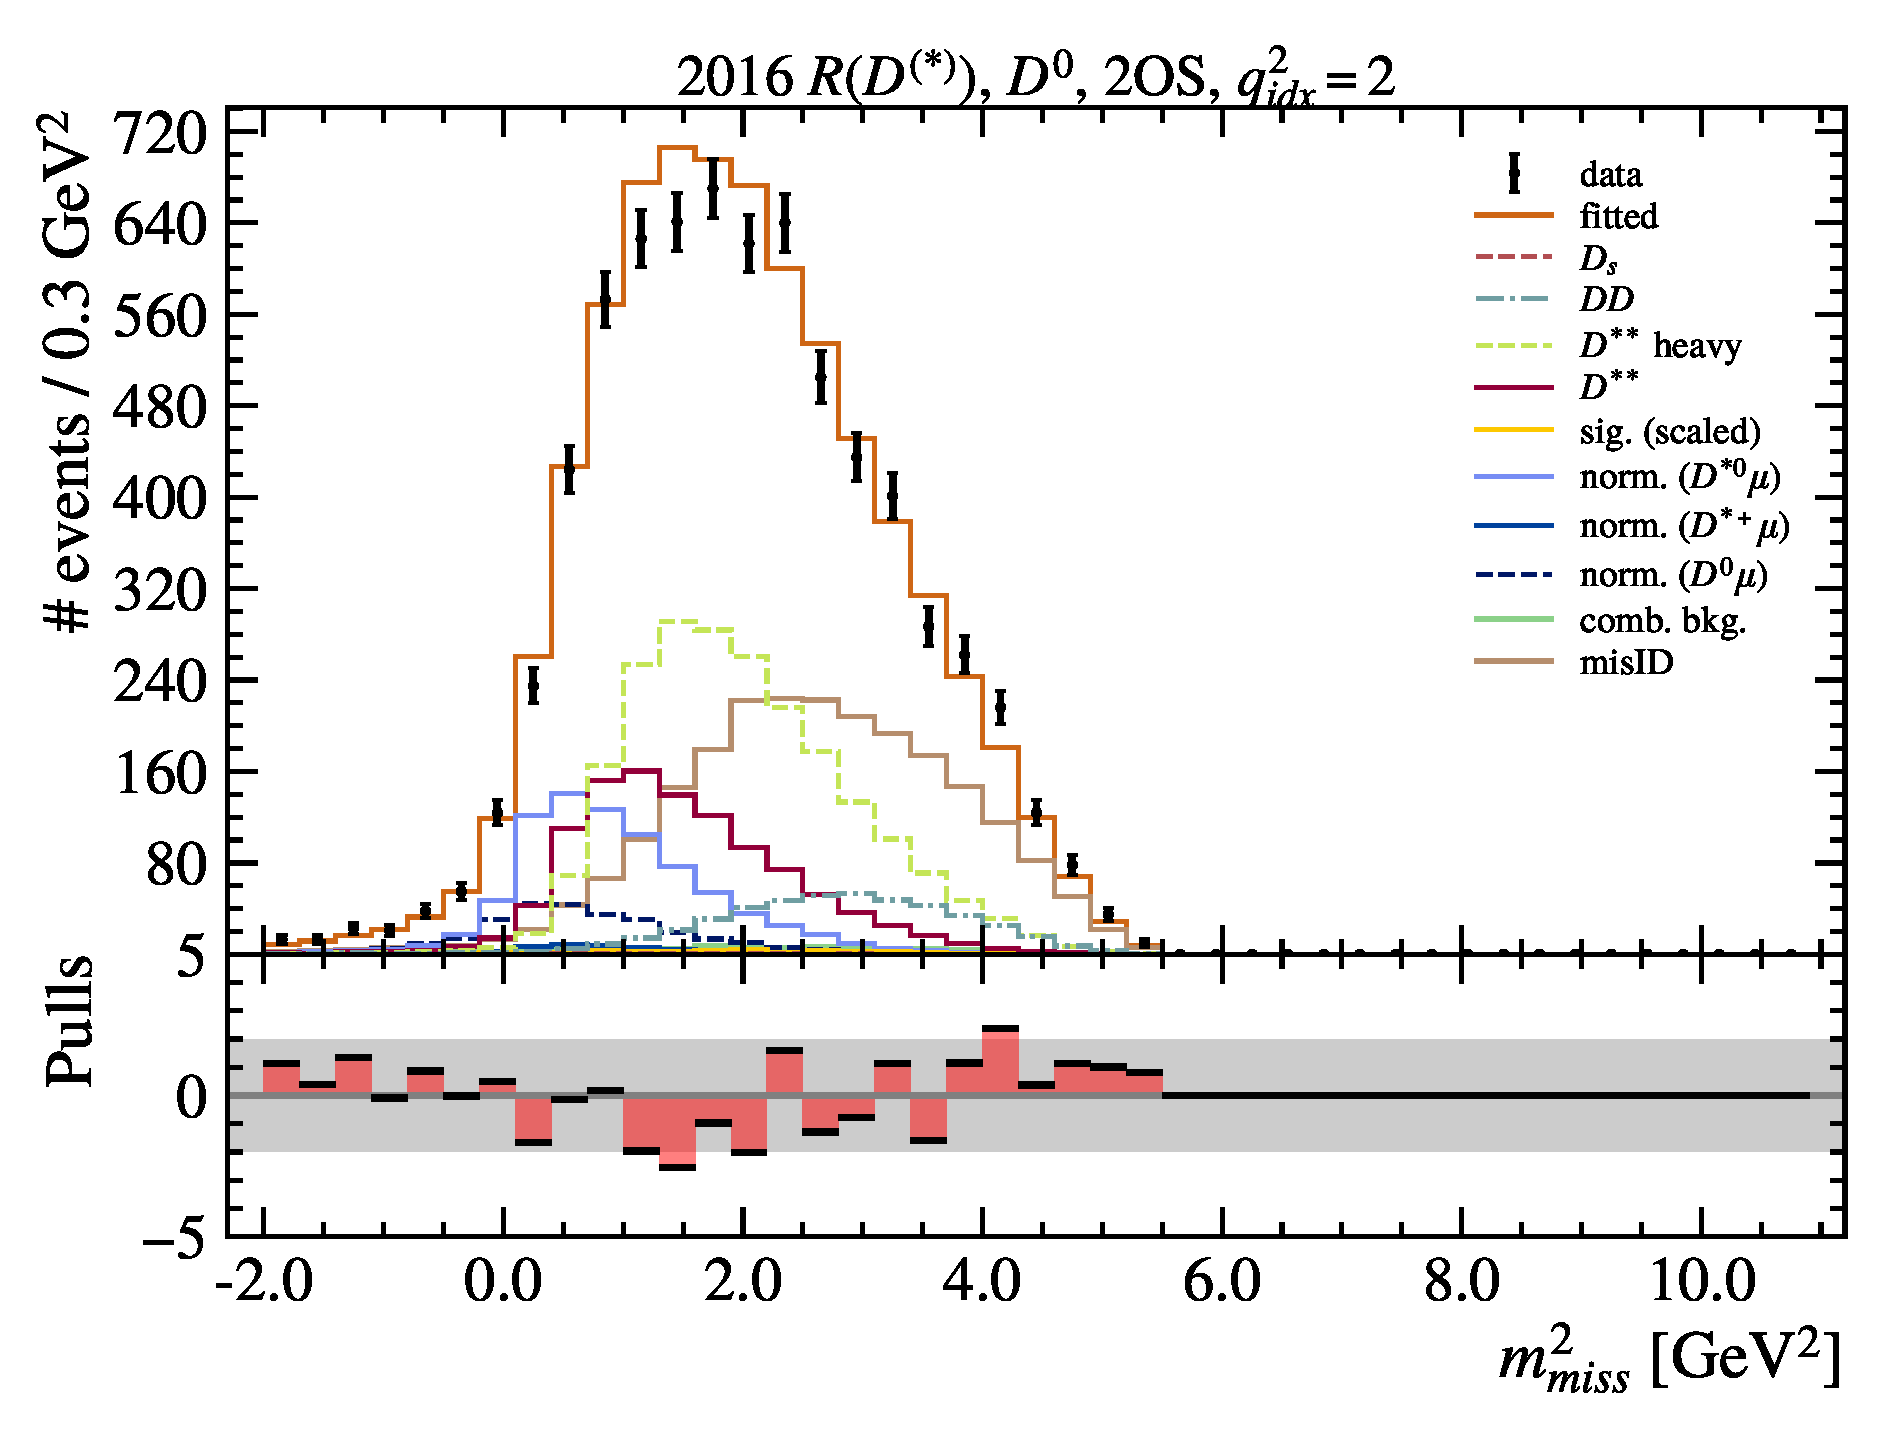
\includegraphics[width=0.24\textwidth]{./figs-fit-fit-results/ctrl-fit/lines_q2_slices/fit_result-lines_q2_idx2-D0-2os-mmiss2.pdf}
    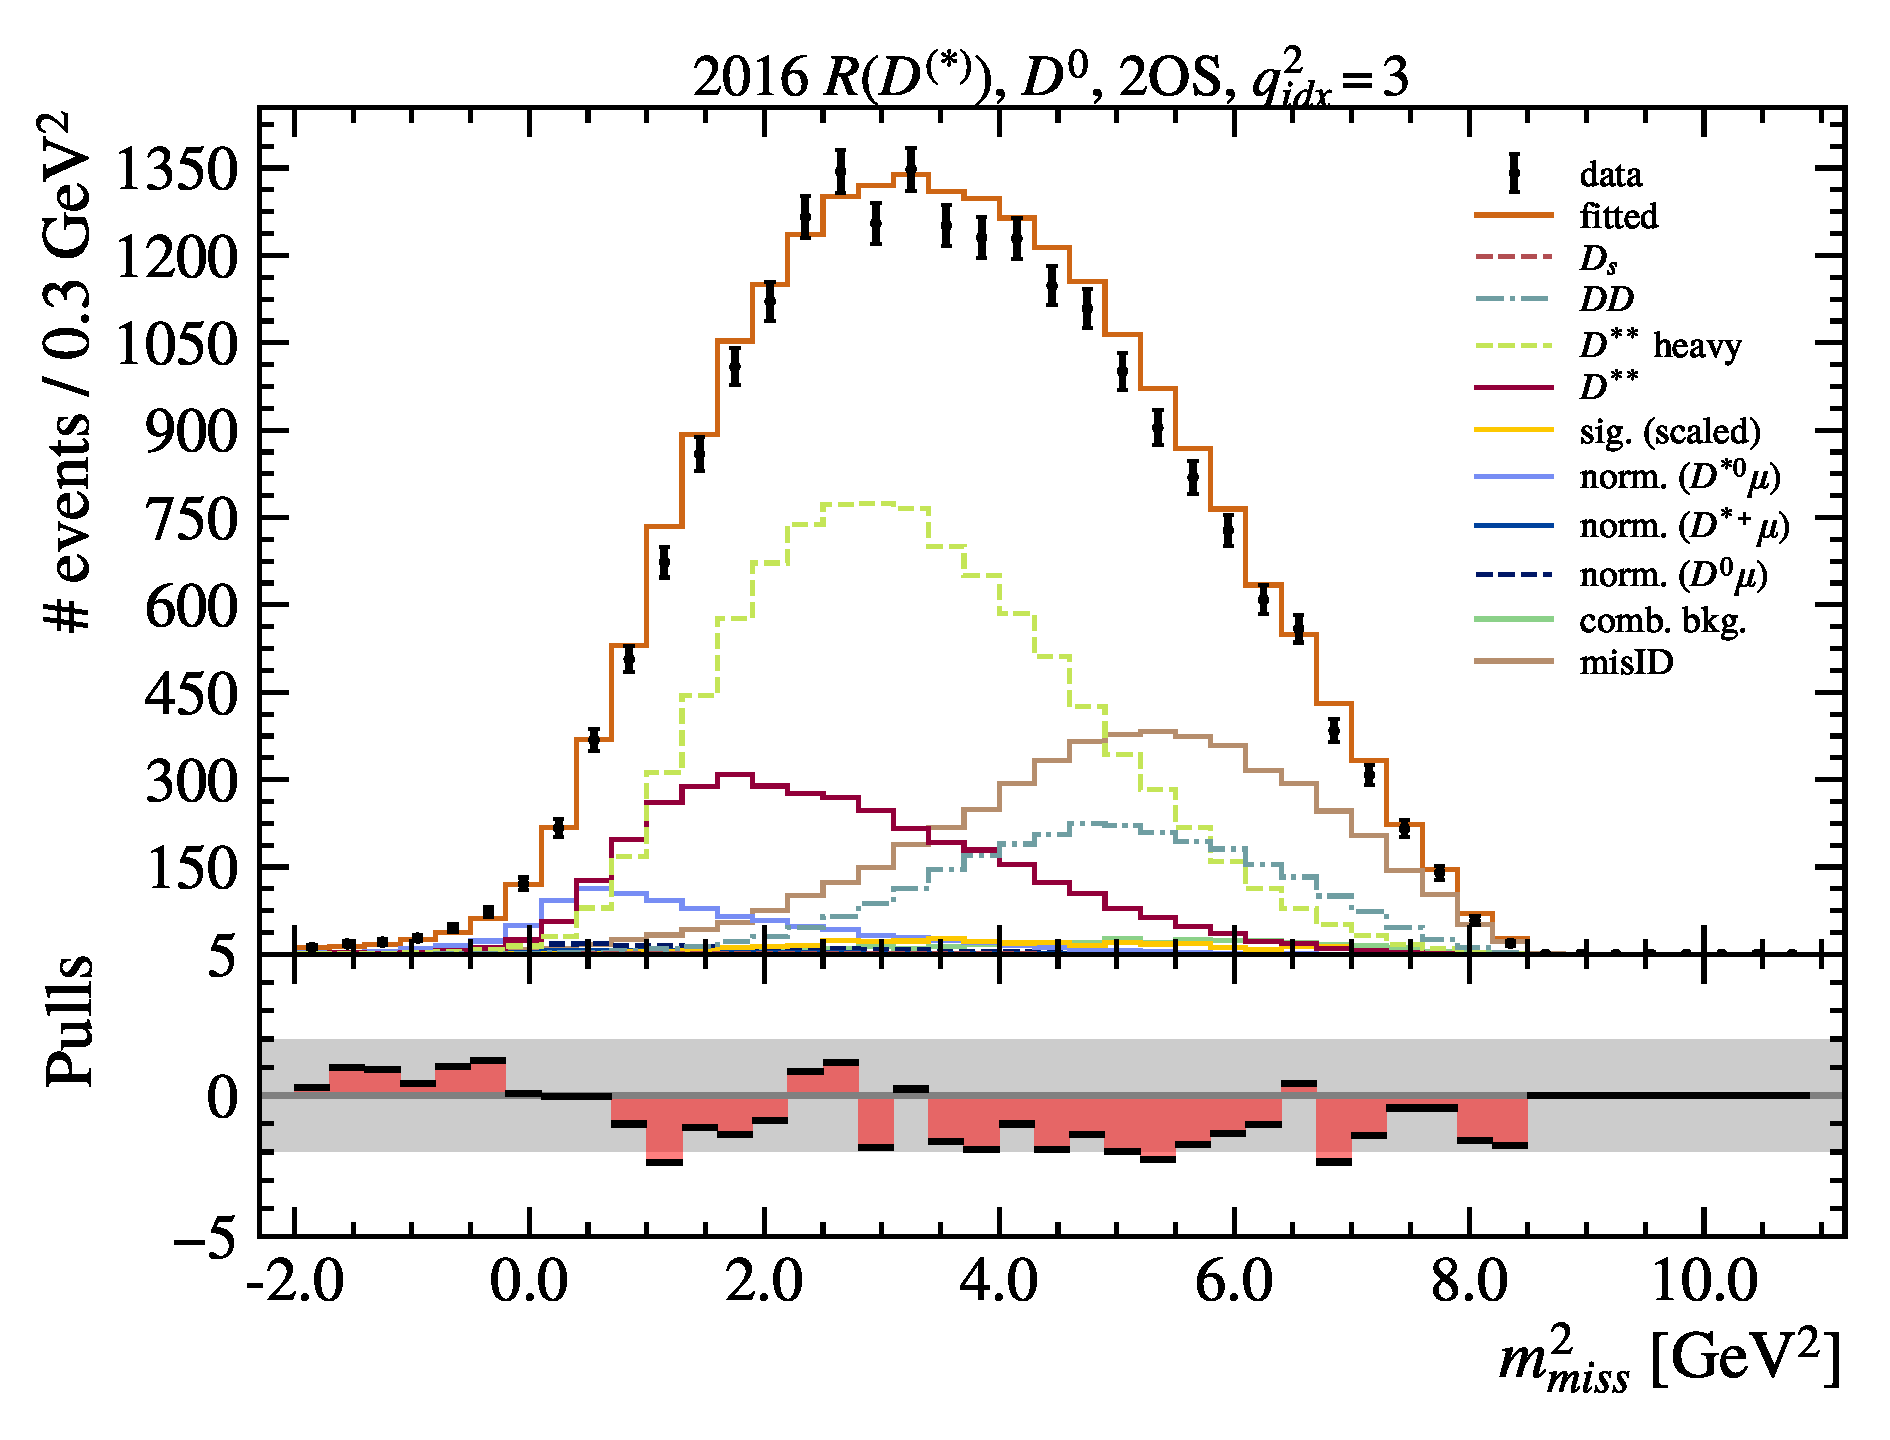
\includegraphics[width=0.24\textwidth]{./figs-fit-fit-results/ctrl-fit/lines_q2_slices/fit_result-lines_q2_idx3-D0-2os-mmiss2.pdf}
    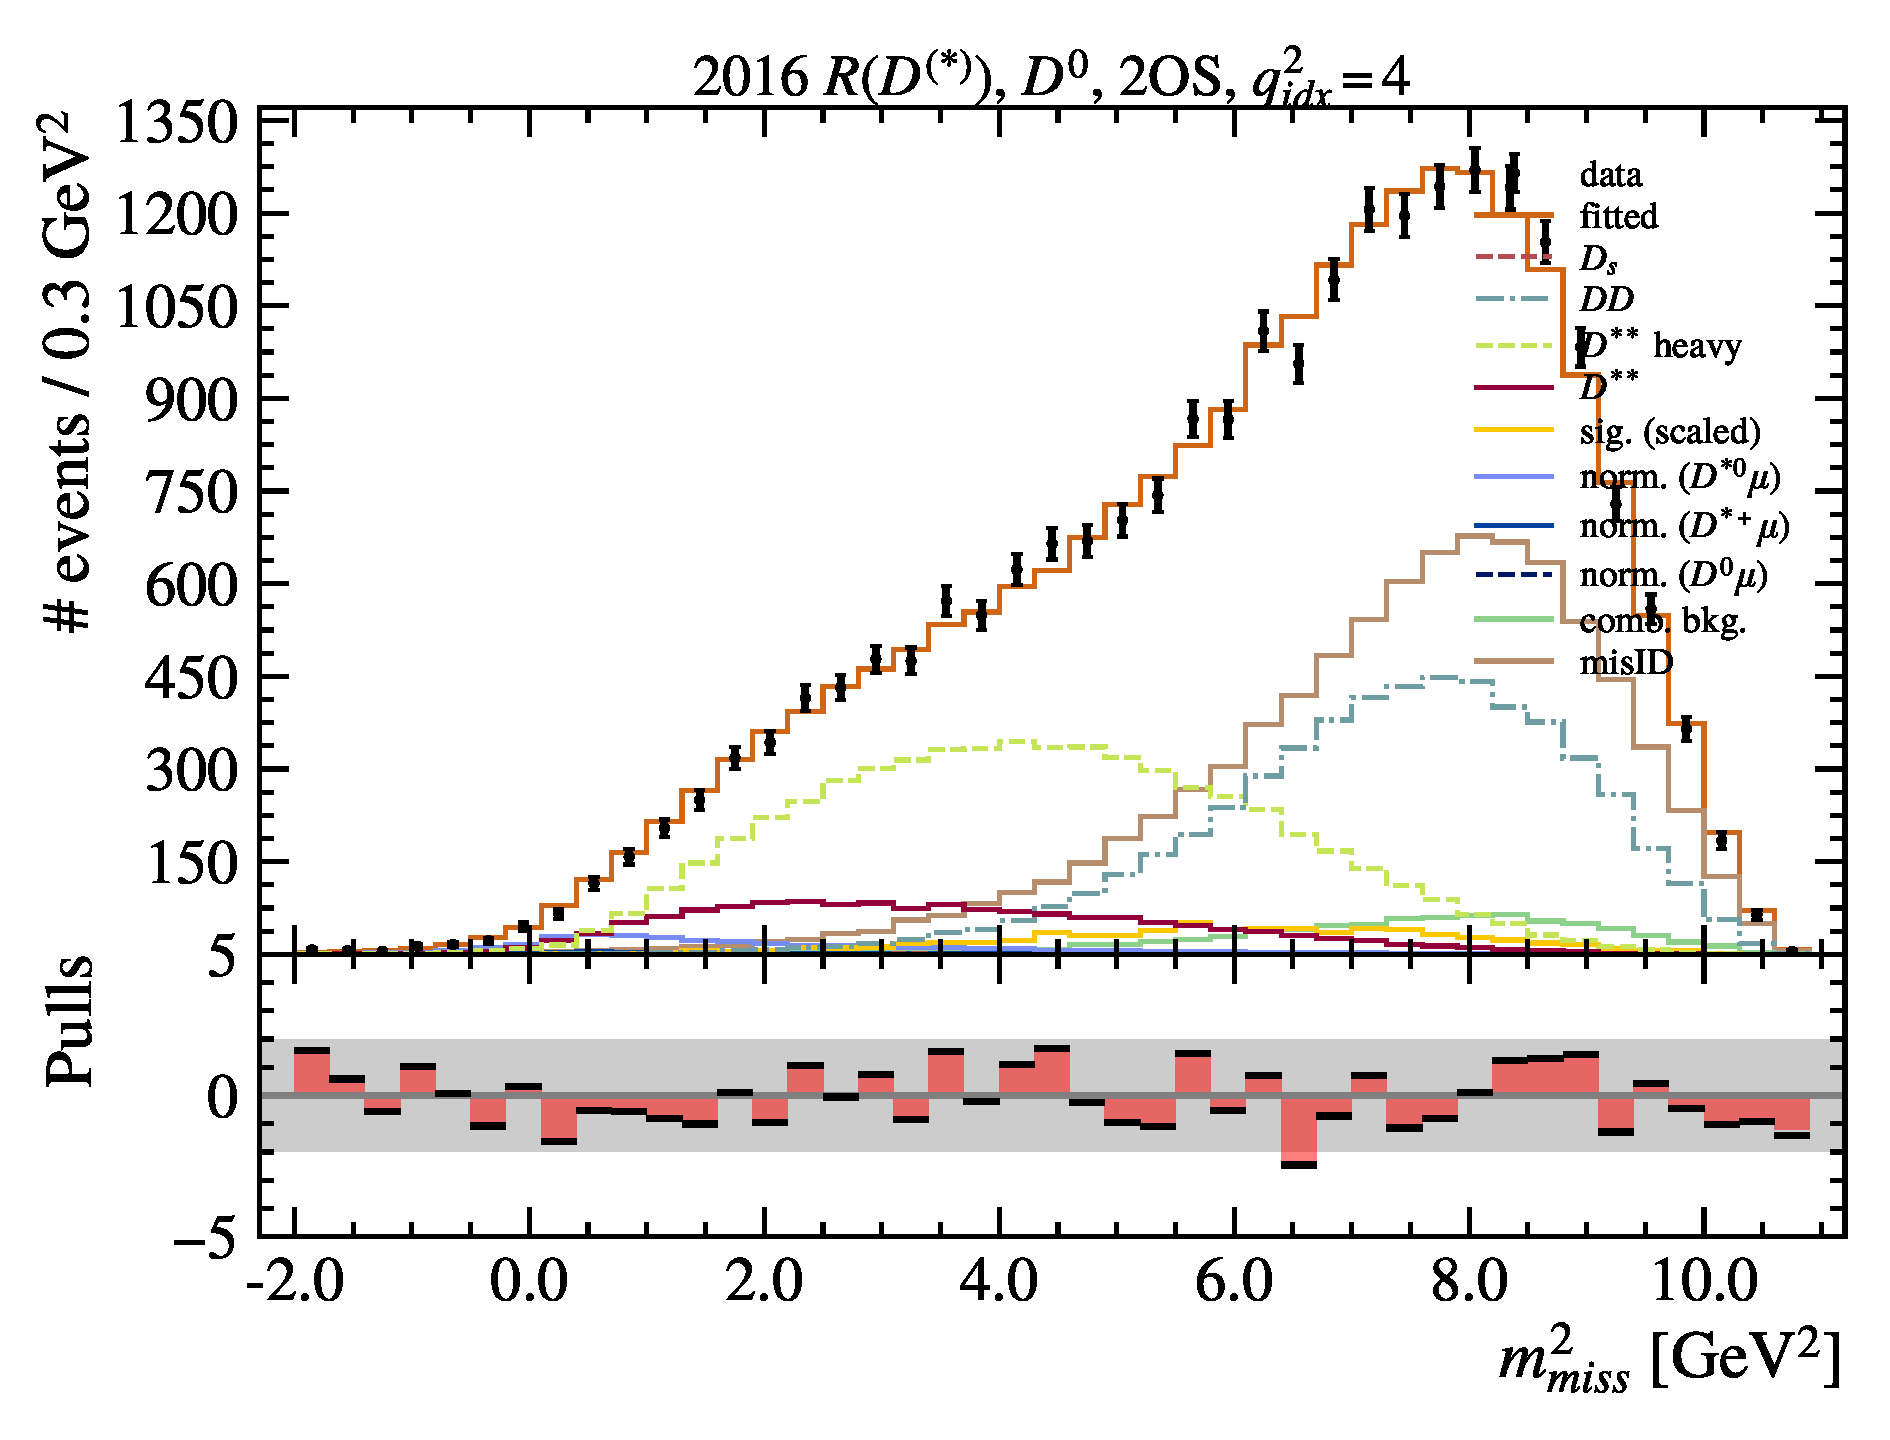
\includegraphics[width=0.24\textwidth]{./figs-fit-fit-results/ctrl-fit/lines_q2_slices/fit_result-lines_q2_idx4-D0-2os-mmiss2.pdf}

    \includegraphics[width=0.24\textwidth]{./figs-fit-fit-results/ctrl-fit/lines_q2_slices/fit_result-lines_q2_idx1-D0-2os-el.pdf}
    \includegraphics[width=0.24\textwidth]{./figs-fit-fit-results/ctrl-fit/lines_q2_slices/fit_result-lines_q2_idx2-D0-2os-el.pdf}
    \includegraphics[width=0.24\textwidth]{./figs-fit-fit-results/ctrl-fit/lines_q2_slices/fit_result-lines_q2_idx3-D0-2os-el.pdf}
    \includegraphics[width=0.24\textwidth]{./figs-fit-fit-results/ctrl-fit/lines_q2_slices/fit_result-lines_q2_idx4-D0-2os-el.pdf}

    \caption{Control fit for 2OS sample, \Dz channel.}
    \label{fig:ctrl-2os-d0}
\end{figure}

\begin{figure}[!htb]
    \centering
    \includegraphics[width=0.32\textwidth]{./figs-fit-fit-results/ctrl-fit/stacked/fit_result-stacked-D0-dd-mmiss2.pdf}
    \includegraphics[width=0.32\textwidth]{./figs-fit-fit-results/ctrl-fit/stacked/fit_result-stacked-D0-dd-el.pdf}
    \includegraphics[width=0.32\textwidth]{./figs-fit-fit-results/ctrl-fit/stacked/fit_result-stacked-D0-dd-q2.pdf}

    \includegraphics[width=0.24\textwidth]{./figs-fit-fit-results/ctrl-fit/lines_q2_slices/fit_result-lines_q2_idx1-D0-dd-mmiss2.pdf}
    \includegraphics[width=0.24\textwidth]{./figs-fit-fit-results/ctrl-fit/lines_q2_slices/fit_result-lines_q2_idx2-D0-dd-mmiss2.pdf}
    \includegraphics[width=0.24\textwidth]{./figs-fit-fit-results/ctrl-fit/lines_q2_slices/fit_result-lines_q2_idx3-D0-dd-mmiss2.pdf}
    \includegraphics[width=0.24\textwidth]{./figs-fit-fit-results/ctrl-fit/lines_q2_slices/fit_result-lines_q2_idx4-D0-dd-mmiss2.pdf}

    \includegraphics[width=0.24\textwidth]{./figs-fit-fit-results/ctrl-fit/lines_q2_slices/fit_result-lines_q2_idx1-D0-dd-el.pdf}
    \includegraphics[width=0.24\textwidth]{./figs-fit-fit-results/ctrl-fit/lines_q2_slices/fit_result-lines_q2_idx2-D0-dd-el.pdf}
    \includegraphics[width=0.24\textwidth]{./figs-fit-fit-results/ctrl-fit/lines_q2_slices/fit_result-lines_q2_idx3-D0-dd-el.pdf}
    \includegraphics[width=0.24\textwidth]{./figs-fit-fit-results/ctrl-fit/lines_q2_slices/fit_result-lines_q2_idx4-D0-dd-el.pdf}

    \caption{Control fit for DD sample, \Dz channel.}
    \label{fig:ctrl-dd-d0}
\end{figure}

\begin{figure}[!htb]
    \centering
    \includegraphics[width=0.32\textwidth]{./figs-fit-fit-results/ctrl-fit/stacked/fit_result-stacked-Dst-1os-mmiss2.pdf}
    \includegraphics[width=0.32\textwidth]{./figs-fit-fit-results/ctrl-fit/stacked/fit_result-stacked-Dst-1os-el.pdf}
    \includegraphics[width=0.32\textwidth]{./figs-fit-fit-results/ctrl-fit/stacked/fit_result-stacked-Dst-1os-q2.pdf}

    \includegraphics[width=0.24\textwidth]{./figs-fit-fit-results/ctrl-fit/lines_q2_slices/fit_result-lines_q2_idx1-Dst-1os-mmiss2.pdf}
    \includegraphics[width=0.24\textwidth]{./figs-fit-fit-results/ctrl-fit/lines_q2_slices/fit_result-lines_q2_idx2-Dst-1os-mmiss2.pdf}
    \includegraphics[width=0.24\textwidth]{./figs-fit-fit-results/ctrl-fit/lines_q2_slices/fit_result-lines_q2_idx3-Dst-1os-mmiss2.pdf}
    \includegraphics[width=0.24\textwidth]{./figs-fit-fit-results/ctrl-fit/lines_q2_slices/fit_result-lines_q2_idx4-Dst-1os-mmiss2.pdf}

    \includegraphics[width=0.24\textwidth]{./figs-fit-fit-results/ctrl-fit/lines_q2_slices/fit_result-lines_q2_idx1-Dst-1os-el.pdf}
    \includegraphics[width=0.24\textwidth]{./figs-fit-fit-results/ctrl-fit/lines_q2_slices/fit_result-lines_q2_idx2-Dst-1os-el.pdf}
    \includegraphics[width=0.24\textwidth]{./figs-fit-fit-results/ctrl-fit/lines_q2_slices/fit_result-lines_q2_idx3-Dst-1os-el.pdf}
    \includegraphics[width=0.24\textwidth]{./figs-fit-fit-results/ctrl-fit/lines_q2_slices/fit_result-lines_q2_idx4-Dst-1os-el.pdf}

    \caption{Control fit for 1OS sample, \Dstar channel.}
    \label{fig:ctrl-1os-dst}
\end{figure}

\begin{figure}[!htb]
    \centering
    \includegraphics[width=0.32\textwidth]{./figs-fit-fit-results/ctrl-fit/stacked/fit_result-stacked-Dst-2os-mmiss2.pdf}
    \includegraphics[width=0.32\textwidth]{./figs-fit-fit-results/ctrl-fit/stacked/fit_result-stacked-Dst-2os-el.pdf}
    \includegraphics[width=0.32\textwidth]{./figs-fit-fit-results/ctrl-fit/stacked/fit_result-stacked-Dst-2os-q2.pdf}

    \includegraphics[width=0.24\textwidth]{./figs-fit-fit-results/ctrl-fit/lines_q2_slices/fit_result-lines_q2_idx1-Dst-2os-mmiss2.pdf}
    \includegraphics[width=0.24\textwidth]{./figs-fit-fit-results/ctrl-fit/lines_q2_slices/fit_result-lines_q2_idx2-Dst-2os-mmiss2.pdf}
    \includegraphics[width=0.24\textwidth]{./figs-fit-fit-results/ctrl-fit/lines_q2_slices/fit_result-lines_q2_idx3-Dst-2os-mmiss2.pdf}
    \includegraphics[width=0.24\textwidth]{./figs-fit-fit-results/ctrl-fit/lines_q2_slices/fit_result-lines_q2_idx4-Dst-2os-mmiss2.pdf}

    \includegraphics[width=0.24\textwidth]{./figs-fit-fit-results/ctrl-fit/lines_q2_slices/fit_result-lines_q2_idx1-Dst-2os-el.pdf}
    \includegraphics[width=0.24\textwidth]{./figs-fit-fit-results/ctrl-fit/lines_q2_slices/fit_result-lines_q2_idx2-Dst-2os-el.pdf}
    \includegraphics[width=0.24\textwidth]{./figs-fit-fit-results/ctrl-fit/lines_q2_slices/fit_result-lines_q2_idx3-Dst-2os-el.pdf}
    \includegraphics[width=0.24\textwidth]{./figs-fit-fit-results/ctrl-fit/lines_q2_slices/fit_result-lines_q2_idx4-Dst-2os-el.pdf}

    \caption{Control fit for 2OS sample, \Dstar channel.}
    \label{fig:ctrl-2os-dst}
\end{figure}

\begin{figure}[!htb]
    \centering
    \includegraphics[width=0.32\textwidth]{./figs-fit-fit-results/ctrl-fit/stacked/fit_result-stacked-Dst-dd-mmiss2.pdf}
    \includegraphics[width=0.32\textwidth]{./figs-fit-fit-results/ctrl-fit/stacked/fit_result-stacked-Dst-dd-el.pdf}
    \includegraphics[width=0.32\textwidth]{./figs-fit-fit-results/ctrl-fit/stacked/fit_result-stacked-Dst-dd-q2.pdf}

    \includegraphics[width=0.24\textwidth]{./figs-fit-fit-results/ctrl-fit/lines_q2_slices/fit_result-lines_q2_idx1-Dst-dd-mmiss2.pdf}
    \includegraphics[width=0.24\textwidth]{./figs-fit-fit-results/ctrl-fit/lines_q2_slices/fit_result-lines_q2_idx2-Dst-dd-mmiss2.pdf}
    \includegraphics[width=0.24\textwidth]{./figs-fit-fit-results/ctrl-fit/lines_q2_slices/fit_result-lines_q2_idx3-Dst-dd-mmiss2.pdf}
    \includegraphics[width=0.24\textwidth]{./figs-fit-fit-results/ctrl-fit/lines_q2_slices/fit_result-lines_q2_idx4-Dst-dd-mmiss2.pdf}

    \includegraphics[width=0.24\textwidth]{./figs-fit-fit-results/ctrl-fit/lines_q2_slices/fit_result-lines_q2_idx1-Dst-dd-el.pdf}
    \includegraphics[width=0.24\textwidth]{./figs-fit-fit-results/ctrl-fit/lines_q2_slices/fit_result-lines_q2_idx2-Dst-dd-el.pdf}
    \includegraphics[width=0.24\textwidth]{./figs-fit-fit-results/ctrl-fit/lines_q2_slices/fit_result-lines_q2_idx3-Dst-dd-el.pdf}
    \includegraphics[width=0.24\textwidth]{./figs-fit-fit-results/ctrl-fit/lines_q2_slices/fit_result-lines_q2_idx4-Dst-dd-el.pdf}

    \caption{Control fit for DD sample, \Dstar channel.}
    \label{fig:ctrl-dd-dst}
\end{figure}


% sig
\begin{figure}[!htb]
    \centering
    \includegraphics[width=0.32\textwidth]{./figs-fit-fit-results/sig-fit/stacked/fit_result-stacked-D0-iso-mmiss2.pdf}
    \includegraphics[width=0.32\textwidth]{./figs-fit-fit-results/sig-fit/stacked/fit_result-stacked-D0-iso-el.pdf}
    \includegraphics[width=0.32\textwidth]{./figs-fit-fit-results/sig-fit/stacked/fit_result-stacked-D0-iso-q2.pdf}

    \includegraphics[width=0.24\textwidth]{./figs-fit-fit-results/sig-fit/lines_q2_slices/fit_result-lines_q2_idx1-D0-iso-mmiss2.pdf}
    \includegraphics[width=0.24\textwidth]{./figs-fit-fit-results/sig-fit/lines_q2_slices/fit_result-lines_q2_idx2-D0-iso-mmiss2.pdf}
    \includegraphics[width=0.24\textwidth]{./figs-fit-fit-results/sig-fit/lines_q2_slices/fit_result-lines_q2_idx3-D0-iso-mmiss2.pdf}
    \includegraphics[width=0.24\textwidth]{./figs-fit-fit-results/sig-fit/lines_q2_slices/fit_result-lines_q2_idx4-D0-iso-mmiss2.pdf}

    \includegraphics[width=0.24\textwidth]{./figs-fit-fit-results/sig-fit/lines_q2_slices/fit_result-lines_q2_idx1-D0-iso-el.pdf}
    \includegraphics[width=0.24\textwidth]{./figs-fit-fit-results/sig-fit/lines_q2_slices/fit_result-lines_q2_idx2-D0-iso-el.pdf}
    \includegraphics[width=0.24\textwidth]{./figs-fit-fit-results/sig-fit/lines_q2_slices/fit_result-lines_q2_idx3-D0-iso-el.pdf}
    \includegraphics[width=0.24\textwidth]{./figs-fit-fit-results/sig-fit/lines_q2_slices/fit_result-lines_q2_idx4-D0-iso-el.pdf}

    \caption{Signal fit for ISO sample, \Dz channel.}
    \label{fig:sig-d0}
\end{figure}

\begin{figure}[!htb]
    \centering
    \includegraphics[width=0.32\textwidth]{./figs-fit-fit-results/sig-fit/stacked/fit_result-stacked-Dst-iso-mmiss2.pdf}
    \includegraphics[width=0.32\textwidth]{./figs-fit-fit-results/sig-fit/stacked/fit_result-stacked-Dst-iso-el.pdf}
    \includegraphics[width=0.32\textwidth]{./figs-fit-fit-results/sig-fit/stacked/fit_result-stacked-Dst-iso-q2.pdf}

    \includegraphics[width=0.24\textwidth]{./figs-fit-fit-results/sig-fit/lines_q2_slices/fit_result-lines_q2_idx1-Dst-iso-mmiss2.pdf}
    \includegraphics[width=0.24\textwidth]{./figs-fit-fit-results/sig-fit/lines_q2_slices/fit_result-lines_q2_idx2-Dst-iso-mmiss2.pdf}
    \includegraphics[width=0.24\textwidth]{./figs-fit-fit-results/sig-fit/lines_q2_slices/fit_result-lines_q2_idx3-Dst-iso-mmiss2.pdf}
    \includegraphics[width=0.24\textwidth]{./figs-fit-fit-results/sig-fit/lines_q2_slices/fit_result-lines_q2_idx4-Dst-iso-mmiss2.pdf}

    \includegraphics[width=0.24\textwidth]{./figs-fit-fit-results/sig-fit/lines_q2_slices/fit_result-lines_q2_idx1-Dst-iso-el.pdf}
    \includegraphics[width=0.24\textwidth]{./figs-fit-fit-results/sig-fit/lines_q2_slices/fit_result-lines_q2_idx2-Dst-iso-el.pdf}
    \includegraphics[width=0.24\textwidth]{./figs-fit-fit-results/sig-fit/lines_q2_slices/fit_result-lines_q2_idx3-Dst-iso-el.pdf}
    \includegraphics[width=0.24\textwidth]{./figs-fit-fit-results/sig-fit/lines_q2_slices/fit_result-lines_q2_idx4-Dst-iso-el.pdf}

    \caption{Signal fit for ISO sample, \Dstar channel.}
    \label{fig:sig-dst}
\end{figure}

